%%%%%% Run at command line, run
%%%%%% xelatex grad-sample.tex 
%%%%%% for a few times to generate the output pdf file
\documentclass[12pt,oneside,openright,a4paper]{cpe-english-project}

 \usepackage{polyglossia}
 \usepackage{float} % for deal with image formatting
 \usepackage{mwe} % for deal with minipage image
 \usepackage{caption} % for deal with captioning the image in minipage
 \usepackage{hyperref} % for deal with inline URL
 \usepackage[table,xcdraw]{xcolor} % for working with the table styling
 \usepackage{multirow}
 \usepackage{longtable}
 \usepackage{url} % for showing the URL in references
 \setdefaultlanguage{english}
 \setotherlanguage{thai}
\newfontfamily\thaifont[Script=Thai,Scale=1.23]{TH Sarabun New}
\defaultfontfeatures{Mapping=tex-text,Scale=1.0,LetterSpace=0.0}
\setmainfont[Scale=1.0,LetterSpace=0,WordSpace=1.0,FakeStretch=1.0]{Times New Roman}
\emergencystretch=10pt
%\XeTeXlinebreaklocale "th_TH"	
%\XeTeXlinebreakskip = 0pt plus 1pt
%\setmathfont(Digits)[Scale=1.0,LetterSpace=0,FakeStretch=1.0]{Times New Roman}


%%%%%%%%%%%%%%%%%%%%%%%%%%%%%%%%%%%%%%%%%%%%%%%%%%%%%%%%%%%%%%%%%%%
% Customize below to suit your needs 
% The ones that are optional can be left blank. 
%%%%%%%%%%%%%%%%%%%%%%%%%%%%%%%%%%%%%%%%%%%%%%%%%%%%%%%%%%%%%%%%%%%
% First line of title
\def\disstitleone{Project G - Educational Game for Learning Genetic Algorithm}   
% Second line of title
%\def\disstitletwo{Project/Indep title line 2 (optional)}   
%% Your first name and lastname
%\def\dissauthor{Mr. Thanapat Mahiskhamin 62070501026 thanapat.mah@mail.kmutt.ac.th}   % 1st member
%%%% Put other group member names here ..
%\def\dissauthortwo{Mr. Pojnarin Nanta 62070501041 pojnarin.nanta@mail.kmutt.ac.th}   % 2nd member (optional)
%\def\dissauthorthree{Mr. Sirapop Apananda 62070503450 sirapop.sk@mail.kmutt.ac.th}   % 3rd member (optional)
% Your first name and lastname
\def\dissauthor{Mr. Thanapat Mahiskhamin}   % 1st member
%%% Put other group member names here ..
\def\dissauthortwo{Mr. Pojnarin Nanta}   % 2nd member (optional)
\def\dissauthorthree{Mr. Sirapop Apananda}   % 3rd member (optional)

% The degree that you're persuing..
\def\dissdegree{Bachelor of Engineering} % Name of the degree
\def\dissdegreeabrev{B.Eng} % Abbreviation of the degree
\def\dissyear{2022}                   % Year of submission
\def\thaidissyear{2565}               % Year of submission (B.E.)

%%%%%%%%%%%%%%%%%%%%%%%%%%%%%%%%%%%%%%%%%%%%
% Your project and independent study committee..
%%%%%%%%%%%%%%%%%%%%%%%%%%%%%%%%%%%%%%%%%%%%
\def\dissadvisor{Assoc.Prof. Natasha Dejdumrong, D.Tech.Sci.}  % Advisor
%%% Leave it empty if you have no Co-advisor
\def\disscoadvisor{Taweechai Nuntawisuttiwong, Ph.D.}  % Co-advisor
\def\disscommitteetwo{Asst.Prof. Suthathip Maneewongvatana, Ph.D.}  % 3rd committee member (optional)
\def\disscommitteethree{Jaturon Harnsomburana, Ph.D.}   % 4th committee member (optional) 

% mid-term committee
%\def\disscommitteetwo{Prapong Prechaprapranwong, Ph.D.}  % 3rd committee member (optional)
%\def\disscommitteethree{Asst.Prof. Suthathip Maneewongvatana, Ph.D.}   % 4th committee member (optional) 
%\def\disscommitteefour{Assoc.Prof. Thumrongrat Amornraksa, Ph.D.}    % 5th committee member (optional) 


\def\worktype{Project} %%  Project or Independent study
\def\disscredit{3}   %% 3 credits or 6 credits


\def\fieldofstudy{Computer Engineering} 
\def\department{Computer Engineering} 
\def\faculty{Engineering}

\def\thaifieldofstudy{วิศวกรรมคอมพิวเตอร์} 
\def\thaidepartment{วิศวกรรมคอมพิวเตอร์} 
\def\thaifaculty{วิศวกรรมศาสตร์}
 
\def\appendixnames{Appendix} %%% Appendices or Appendix

\def\thaiworktype{ปริญญานิพนธ์} %  Project or research project % 
\def\thaidisstitleone{Project G - Educational Game for Learning Genetic Algorithm}
\def\thaidisstitletwo{}
\def\thaidissauthor{นายธนภัทร มหิษคามิน}
\def\thaidissauthortwo{นายพจนรินทร์ นันตะ} %Optional
\def\thaidissauthorthree{นายสิรภพ อปานนท์} %Optional

\def\thaidissadvisor{รศ.ดร. ณัฐชา เดชดำรง}
%% Leave this empty if you have no co-advisor
\def\thaidisscoadvisor{ดร. ทวีชัย นันทวิสุทธิวงศ์} %Optional
\def\thaidissdegree{วิศวกรรมศาสตรบัณฑิต}

% Change the line spacing here...
\linespread{1.15}

%%%%%%%%%%%%%%%%%%%%%%%%%%%%%%%%%%%%%%%%%%%%%%%%%%%%%%%%%%%%%%%%
% End of personal customization.  Do not modify from this part 
% to \begin{document} unless you know what you are doing...
%%%%%%%%%%%%%%%%%%%%%%%%%%%%%%%%%%%%%%%%%%%%%%%%%%%%%%%%%%%%%%%%


%%%%%%%%%%%% Dissertation style %%%%%%%%%%%
%\linespread{1.6} % Double-spaced  
%%\oddsidemargin    0.5in
%%\evensidemargin   0.5in
%%%%%%%%%%%%%%%%%%%%%%%%%%%%%%%%%%%%%%%%%%%
%\renewcommand{\subfigtopskip}{10pt}
%\renewcommand{\subfigbottomskip}{-5pt} 
%\renewcommand{\subfigcapskip}{-6pt} %vertical space between caption
%                                    %and figure.
%\renewcommand{\subfigcapmargin}{0pt}

\renewcommand{\topfraction}{0.85}
\renewcommand{\textfraction}{0.1}

\newtheorem{theorem}{Theorem}
\newtheorem{lemma}{Lemma}
\newtheorem{corollary}{Corollary}

\def\QED{\mbox{\rule[0pt]{1.5ex}{1.5ex}}}
\def\proof{\noindent\hspace{2em}{\itshape Proof: }}
\def\endproof{\hspace*{\fill}~\QED\par\endtrivlist\unskip}
%\newenvironment{proof}{{\sc Proof:}}{~\hfill \blacksquare}
%% The hyperref package redefines the \appendix. This one 
%% is from the dissertation.cls
%\def\appendix#1{\iffirstappendix \appendixcover \firstappendixfalse \fi \chapter{#1}}
%\renewcommand{\arraystretch}{0.8}
%%%%%%%%%%%%%%%%%%%%%%%%%%%%%%%%%%%%%%%%%%%%%%%%%%%%%%%%%%%%%%%%
%%%%%%%%%%%%%%%%%%%%%%%%%%%%%%%%%%%%%%%%%%%%%%%%%%%%%%%%%%%%%%%%


\begin{document}
\pdfstringdefDisableCommands{%
\let\MakeUppercase\relax
}
\begin{center}
  
\includegraphics[width=2.8cm]{logo02.png}
\end{center}
\vspace*{-1cm}

\maketitlepage
\makesignaturepage 

%%%%%%%%%%%%%%%%%%%%%%%%%%%%%%%%%%%%%%%%%%%%%%%%%%%%%%%%%%%%%%%
%%%%%%%%%%%%%%%%%%%%%%% English abstract %%%%%%%%%%%%%%%%%%%%%%%
%%%%%%%%%%%%%%%%%%%%%%%%%%%%%%%%%%%%%%%%%%%%%%%%%%%%%%%%%%%%%%%
\abstract

Nowadays, education is not explicitly conducted in a classroom anymore. Everybody can gain new knowledge about anything at any time they want. Various media are also adjusted to fit diverse target groups; one of the most popular formats is the educational game. \\
Project G - Educational Game for Learning Genetic Algorithm was built with the intention of providing players knowledge about the Genetic Algorithm and the Knapsack Problem through the game, as it can be both entertaining and academic at the same time. It can also evaluate players with various methods. Its training methods through puzzles will give players more understanding of those topics. \\
In this game, players will roleplay as mech company owners, using the Genetic Algorithm in the mech and weapon production. Players have to learn and use the knowledge to manage the facilities. Above that, there are more activities for players, such as fixing facilities, producing mechs according to customers’ requests, and using mechs to battle and earn rewards.


\begin{flushleft}
\begin{tabular*}{\textwidth}{@{}lp{0.8\textwidth}}
\textbf{Keywords}:  Computer Game / Genetic Algorithm / Educational / Breeding Simulation / Resource \\Management / Puzzle
\end{tabular*}
\end{flushleft}
\endabstract

%%%%%%%%%%%%%%%%%%%%%%%%%%%%%%%%%%%%%%%%%%%%%%%%%%%%%%%%%%%%%%
%%%%%%%%%% Thai abstract here %%%%%%%%%%%%%%%%%%%%%%%%%%%%%%%%%
%%%%%%%%%%%%%%%%%%%%%%%%%%%%%%%%%%%%%%%%%%%%%%%%%%%%%%%%%%%%%%
{
%\begin{thai}
\XeTeXlinebreaklocale "th_TH"	
\XeTeXlinebreakskip = 0pt plus 1pt
\thaifont
\thaiabstract

ในปัจจุบัน การเรียนรู้นั้นไม่ถูกจำกัดอยู่ภายในห้องเรียนอีกต่อไป ทุกคนสามารถหาความรู้ได้อย่างรวดเร็วและง่ายดายกว่าเดิม สื่อต่าง ๆ สามารถเข้าถึงได้เพียงเชื่อมต่ออินเทอร์เน็ต ยิ่งไปกว่านั้น สื่อการเรียนรู้เองก็ได้มีการพัฒนาให้มีความหลากหลายให้เหมาะกับกลุ่มเป้าหมายต่าง ๆ และหนึ่งในรูปแบบที่ถูกจับตามองก็คือเกมเพื่อการศึกษานั่นเอง \\
Project G - Educational Game for Learning Genetic Algorithm นั้นถูกจัดทำขึ้นโดยมีจุดประสงค์เพื่อมอบความรู้เชิงวิชาการเกี่ยวกับอัลกอริธึมเชิงพันธุกรรมและปัญหาถุงกระสอบให้กับผู้ที่สนใจผ่านรูปแบบเกมซึ่งเป็นสื่อที่สามารถมอบทั้งความรู้และความสนุกให้กับผู้เล่น พร้อมทั้งสามารถวัดผลการเรียนรู้ออกมาได้ผ่านวิธีการต่าง ๆ และมีวิธีการสอนและทบทวนผ่านการแก้ปริศนาซึ่งสามารถช่วยให้ผู้เล่นเข้าใจหลักการของอัลกอริธึมได้ดียิ่งขึ้น \\
ตัวเกมจะให้ผู้เล่นได้สวมบทบาทเป็นเจ้าของโรงงานพัฒนาหุ่นยนต์ซึ่งมีวิธีการพัฒนาหุ่นยนต์และอาวุธด้วยอัลกอริธึมเชิงพันธุกรรม โดยผู้เล่นจะต้องเรียนรู้หลักการทำงานของมันและใช้ความรู้ที่มีประกอบการบริหารโรงงานได้ ซึ่งมีกิจกรรมต่าง ๆ ให้ผู้เล่นได้ทำ เช่นการทำนุบำรุงโรงงาน การผลิตหุ่นยนต์ให้ตรงตามความต้องการของลูกค้า หรือการนำหุ่นยนต์ในโรงงานไปต่อสู้เพื่อชิงเงินรางวัล


\begin{flushleft}
\begin{tabular*}{\textwidth}{@{}lp{0.8\textwidth}}
 & \\

\textbf{คำสำคัญ}: เกมคอมพิวเตอร์ / อัลกอริธึมเชิงพันธุกรรม / การศึกษา / การจำลองการผสมพันธุ์ / การจัดการทรัพยากร / ปริศนา
\end{tabular*}
\end{flushleft}
\endabstract
%\end{thai}
}

%%%%%%%%%%%%%%%%%%%%%%%%%%%%%%%%%%%%%%%%%%%%%%%%%%%%%%%%%%%%
%%%%%%%%%%%%%%%%%%%%%%% Acknowledgments %%%%%%%%%%%%%%%%%%%%
%%%%%%%%%%%%%%%%%%%%%%%%%%%%%%%%%%%%%%%%%%%%%%%%%%%%%%%%%%%%
\preface

First, we would like to thank our advisors, Assoc.Prof.Dr. Natasha Dejdumrong and Dr. Taweechai Nuntawisuttiwong, for giving us various advice and sharing their knowledge about game development and other crucial things to make this project happen. \\
Next, we sincerely appreciate the help of every committee for commenting and setting our project on the right path. There were multiple issues that we overlooked in the project, and we would not notice them without the wit of the committees. \\
We are truly grateful for our 92 play-testers sacrificing their own time to test our game and submit numerous helpful feedback from the perspectives of the player that we developers might ignore to improve our game. \\
In addition to those mentioned earlier, we are thankful to ChatGPT for providing us with many helpful and creative opinions, and supporting us in diverse fields throughout the project. Arknights is thanked for giving us ideas and inspiration about how the developers care about their game and players. \\
Finally, we thank the capybaras for being such cute creatures and providing us with the motivation to start and finish this project. This gratitude extends to the natural selection and evolution that make capybaras exist on this planet. We genuinely appreciate that.


%%%%%%%%%%%%%%%%%%%%%%%%%%%%%%%%%%%%%%%%%%%%%%%%%%%%%%%%%%%%%
%%%%%%%%%%%%%%%% ToC, List of figures/tables %%%%%%%%%%%%%%%%
%%%%%%%%%%%%%%%%%%%%%%%%%%%%%%%%%%%%%%%%%%%%%%%%%%%%%%%%%%%%%
% The three commands below automatically generate the table 
% of content, list of tables and list of figures
\tableofcontents                    
\listoftables
\listoffigures                      

%%%%%%%%%%%%%%%%%%%%%%%%%%%%%%%%%%%%%%%%%%%%%%%%%%%%%%%%%%%%%%%
%%%%%%%%%%%%%%%%%%%%%% List of symbols page %%%%%%%%%%%%%%%%%%%
%%%%%%%%%%%%%%%%%%%%%%%%%%%%%%%%%%%%%%%%%%%%%%%%%%%%%%%%%%%%%%%
%% You have to add this manually..
%\listofsymbols
%\begin{flushleft}
%\begin{tabular}{@{}p{0.07\textwidth}p{0.7\textwidth}p{0.1\textwidth}}
%\textbf{SYMBOL}  & & \textbf{UNIT} \\[0.2cm]
%$\alpha$ & Test variable\hfill & m$^2$ \\
%$\lambda$ & Interarival rate\hfill &  jobs/second\\
%$\mu$ & Service rate\hfill & jobs/second\\
%\end{tabular}
%\end{flushleft}
%%%%%%%%%%%%%%%%%%%%%%%%%%%%%%%%%%%%%%%%%%%%%%%%%%%%%%%%%%%%%%%
%%%%%%%%%%%%%%%%%%%%%% List of vocabs & terms %%%%%%%%%%%%%%%%%
%%%%%%%%%%%%%%%%%%%%%%%%%%%%%%%%%%%%%%%%%%%%%%%%%%%%%%%%%%%%%%%
%% You also have to add this manually..
%\listofvocab
%\begin{flushleft}
%\begin{tabular}{@{}p{1in}@{=\extracolsep{0.5in}}l}
%ABC & Adaptive Bandwidth Control \\
%MANET & Mobile Ad Hoc Network 
%\end{tabular}
%\end{flushleft}
%
%\setlength{\parskip}{1.2mm}



%%%%%%%%%%%%%%%%%%%%%%%%%%%%%%%%%%%%%%%%%%%%%%%%%%%%%%%%%%%%%%%%%
%%%%%%%%%%%%%%%%%%%%%%% Main body %%%%%%%%%%%%%%%%%%%%%%%%%%%%%%%%%%%%
%%%%%%%%%%%%%%%%%%%%%%%%%%%%%%%%%%%%%%%%%%%%%%%%%%%%%%%%%%%%%%%%%
\chapter{Introduction}
\hspace{2em}In this chapter, we will describe the basic information of the project including background, objectives, scope of work, and project schedule.


%%%%%%%%%%%%%%%%%%%%%%%%%%%%%%%%%%%%%%%%%%%%%%%%%%%%%%%%%%%%%%%%%
%%%%%%%%%%%%%%%%%%%%%%%%%%%%%%%%%%%%%%%%%%%%%%%%%%%%%%%%%%%%%%%%%
\section{Background} 
\hspace{2em}Nowadays, human technologies have been growing exponentially with no sign of slowing down; with the ongoing pandemic, many things have shifted to the digital world, disrupting older technologies and forcing people in this generation to improvise, adapt, and overcome their capabilities. One of the constantly-evolving technologies is the game industry.

\hspace{2em}In recent years, computer games have been getting more attention from the public as the game industry has been rapidly elevating nonstop. Usually, these media get acknowledged as relaxing activities; however, they also have great potential as learning tools \cite{gomez2022academic}. They are easy to access by nearly everyone, especially younger generations who are accustomed to computers and technologies. Furthermore, they can easily get caught by entertainment media; games can serve as tools for education for them. There are lots of educational games coming out, and they cover almost every topic, from simple language or first-grade math to physics, chemistry, and computer science.

\hspace{2em}With the rapid growth of technologies and knowledge, education has become more radical than ever; to catch up with everything. Since the popularity of computer games is increasing, the interest in learning computer engineering is increasing. However, some content in this field is hard to study, for example, the Genetic Algorithm. Integrating knowledge about the Genetic Algorithm with computer games provides friendlier ways to access and understand the Genetic Algorithm.

\hspace{2em}An article suggests there is currently no academic game teaching about the Genetic Algorithm \cite{udeozor2022digital}. After some consideration, research, planning, and designing, our group proposed an educational game to educate the players, simulate how the Genetic Algorithm works, and present them to the audiences in an interactive media with the story and incentive to play. To help and motivate them to have more understanding of the said topic, we use puzzle and breeding simulator genres with the design of outcome-based education for teaching, evaluation, and education. We also use role-playing and auto-battler genres with a game design theory to motivate the players and let them have fun while playing the game. Using games as a medium for education encourages players to have the motivation and focus by giving engaging gameplay and pleasing visual and audio aesthetics to the players \cite{plass2015foundations}.


%%%%%%%%%%%%%%%%%%%%%%%%%%%%%%%%%%%%%%%%%%%%%%%%%%%%%%%%%%%%%%%%%%
%%%%%%%%%%%%%%%%%%%%%%%%%%%%%%%%%%%%%%%%%%%%%%%%%%%%%%%%%%%%%%%%%%
%\section{Motivations}
%Explain the motivations of your works.  
%\begin{itemize}
%\item   What are the problems you are addressing? 
%\item  Why they are important?
%\item  What are the limitations of existing approaches? 
%\end{itemize}
%You may combine this section with the background section.
%
%
%%%%%%%%%%%%%%%%%%%%%%%%%%%%%%%%%%%%%%%%%%%%%%%%%%%%%%%%%%%%%%%%%%
%%%%%%%%%%%%%%%%%%%%%%%%%%%%%%%%%%%%%%%%%%%%%%%%%%%%%%%%%%%%%%%%%%
%\section{Problem Statements}
%Capybara


%%%%%%%%%%%%%%%%%%%%%%%%%%%%%%%%%%%%%%%%%%%%%%%%%%%%%%%%%%%%%%%%%
%%%%%%%%%%%%%%%%%%%%%%%%%%%%%%%%%%%%%%%%%%%%%%%%%%%%%%%%%%%%%%%%%
\section{Objectives}
As said before, these objectives are separated into two parts, those for the organizers; and those for players.
\begin{enumerate}
	\item To study and research Unity engine, C\#, and the Genetic Algorithm.
	\item To make a simple educational game for people who want to learn about the Genetic Algorithm.
	\item To research and apply the Genetic Algorithm in the game-making field.
	\item To assist players in practicing making and planning decisions and managing resources.
\end{enumerate}


%%%%%%%%%%%%%%%%%%%%%%%%%%%%%%%%%%%%%%%%%%%%%%%%%%%%%%%%%%%%%%%%%
%%%%%%%%%%%%%%%%%%%%%%%%%%%%%%%%%%%%%%%%%%%%%%%%%%%%%%%%%%%%%%%%%
\section{Scope of Work}
In this part, we will list system requirements, systems included in the project, and educational topics we will cover.
\begin{enumerate}
	\item Windows-supported game developed using Unity.
	\item In-game System
	\begin{enumerate}
		\item Breeding Farm \\
		Simulating monster breeding using the Genetic Algorithm. The system consists of breeding farms and habitats. The breeding can only be done on breeding farms.
		\item Weapon Factory \\
		Using the Knapsack problem as a weapon creation. There are 5 factories in total.
		\item Research Lab \\
		The system where players must learn and test their knowledge about the Genetic Algorithm to unlock other new facilities.
		\item Miscellaneous
		\begin{enumerate}
			\item Shop \\
			The place where players can spend their money to buy more monsters or weapons to use in their farms and factories.
			\item Time progression \\
			The system allows players to renew the content in quest, arena and skip past the times used for the breeding process.
			\item Money  \\
			The currency for buying more resources for the farms and factories, fixing the broken parts and breeding monsters or weapons to make a new generation.
			\item Arena \\
			The system for players to earn money by using their monsters and weapons to fight the randomly generated enemies.
			\item Quest \\
			The system for players to earn money by sending their monsters or weapons that match the requested monsters. The amount of money that players earn depends on the grading of how similar between the sent monsters and the requested monsters.
		\end{enumerate}
	\end{enumerate}
	\item Educational topic
	\begin{enumerate}
		\item Genetic Algorithms
		\begin{enumerate}
			\item Selection
			\begin{enumerate}
				\item Random Selection
				\item Tournament-based Selection
				\item Roulette Wheel Selection
				\item Rank-based Selection
				\item Elitism
			\end{enumerate}
			\item Crossover
			\begin{enumerate}
				\item Single-point Crossover
				\item Two-point Crossover
				\item Uniform Crossover
			\end{enumerate}
			\item Mutation
			\begin{enumerate}
				\item Bit Flip Mutation
				\item Flip Bit Mutation
				\item Boundary Mutation
			\end{enumerate}
		\end{enumerate}
		\item Real-world problems
		\begin{enumerate}
			\item Standard Knapsack Problem
			\item Multidimensional Knapsack Problem
			\item Multiple Knapsack Problem
		\end{enumerate}
	\end{enumerate}
\end{enumerate}

%Explain the scope of your works. 
%\begin{itemize}
%\item   What are the problems you are addressing? 
%\item  Why they are important?
%\item  What are the limitations of existing approaches? 
%\end{itemize}


%%%%%%%%%%%%%%%%%%%%%%%%%%%%%%%%%%%%%%%%%%%%%%%%%%%%%%%%%%%%%%%%%
%%%%%%%%%%%%%%%%%%%%%%%%%%%%%%%%%%%%%%%%%%%%%%%%%%%%%%%%%%%%%%%%%
\section{Project Schedule}
We use Scrum as a development process. We will list details about development activities, product backlog, and draft schedule.

%%%%%%%%%%%%%%%%%%%%%%%%%%%%%%%%%%%%%%%%%%%%%%%%%%%%%%%%%%%%%%%%%
\subsection{Development Activities}
Within the Scrum process, there are 3 important activities which are Sprint, Weekly Meeting, and Sprint Review.

\begin{enumerate}
	\item Sprint \\
	All development processes are divided into nine 3-week sprints. The total estimated effort for each sprint is roughly equal to 27 man-half-days.
	\item Weekly Meeting \\
	Meeting 15 minutes or less, repeatedly on Friday, when each member has their own responsibilities. The members report their own accomplishments, will accomplish, and Impediments.
	\item Sprint Review \\
	Meeting at the end of each Sprint, 3 hours or less, to review completed tasks, design artifacts, and adjust Backlog and plans for the next Sprint.
\end{enumerate}

%%%%%%%%%%%%%%%%%%%%%%%%%%%%%%%%%%%%%%%%%%%%%%%%%%%%%%%%%%%%%%%%%
\subsection{Product Backlog}
We will list the task breakdown in a form of the product backlog. This also includes the priority and the estimated effort for doing each task.
% sprint backlog table generated from an online table generator

% Please add the following required packages to your document preamble:
% \usepackage[table,xcdraw]{xcolor}
% If you use beamer only pass "xcolor=table" option, i.e. \documentclass[xcolor=table]{beamer}
\begin{table}[!h]
\centering
\caption{Product Backlog}
\label{tbl:product-backlog}
\begin{tabular}{|ll|c|c|}
\hline
\rowcolor[HTML]{EFEFEF} 
\multicolumn{1}{|c|}{\cellcolor[HTML]{EFEFEF}ID} & \multicolumn{1}{c|}{\cellcolor[HTML]{EFEFEF}Story}                           & \begin{tabular}[c]{@{}c@{}}Effort Estimate\\ (Man-Half-Days)\end{tabular} & Priority \\ \hline
\multicolumn{1}{|c|}{1}                          & Developers need to do project documents.                                     & 36                                                                        & 1        \\ \hline
\multicolumn{1}{|c|}{2}                          & Players can learn about the Genetic Algorithm.                               & 36                                                                        & 2        \\ \hline
\multicolumn{1}{|c|}{3}                          & Players can apply knowledge to solve real-world problems.                    & 32                                                                        & 3        \\ \hline
\multicolumn{1}{|l|}{4}                          & Players can breed their monsters.                                            & 20                                                                        & 4        \\ \hline
\multicolumn{1}{|l|}{5}                          & Players have mandatory goals for playing a game.                             & 12                                                                        & 5        \\ \hline
\multicolumn{1}{|l|}{6}                          & Players have other activities to spend their time during the breeding phase. & 32                                                                        & 6        \\ \hline
\multicolumn{1}{|l|}{7}                          & Developers integrate all the systems.                                        & 20                                                                        & 7        \\ \hline
\multicolumn{1}{|l|}{8}                          & Developers add more aesthetics to the game.                                  & 32                                                                        & 8        \\ \hline
\multicolumn{1}{|l|}{9}                          & Developers assure quality.                                                   & 20                                                                        & 9        \\ \hline
\multicolumn{2}{|l|}{Total}                                                                                                     & 240                                                                       &          \\ \hline
\end{tabular}
\end{table}

%%%%%%%%%%%%%%%%%%%%%%%%%%%%%%%%%%%%%%%%%%%%%%%%%%%%%%%%%%%%%%%%%
\subsection{Draft Schedule}
The draft schedule of the Sprints will be shown as follows.

\begin{minipage}[c]{\textwidth}\centering
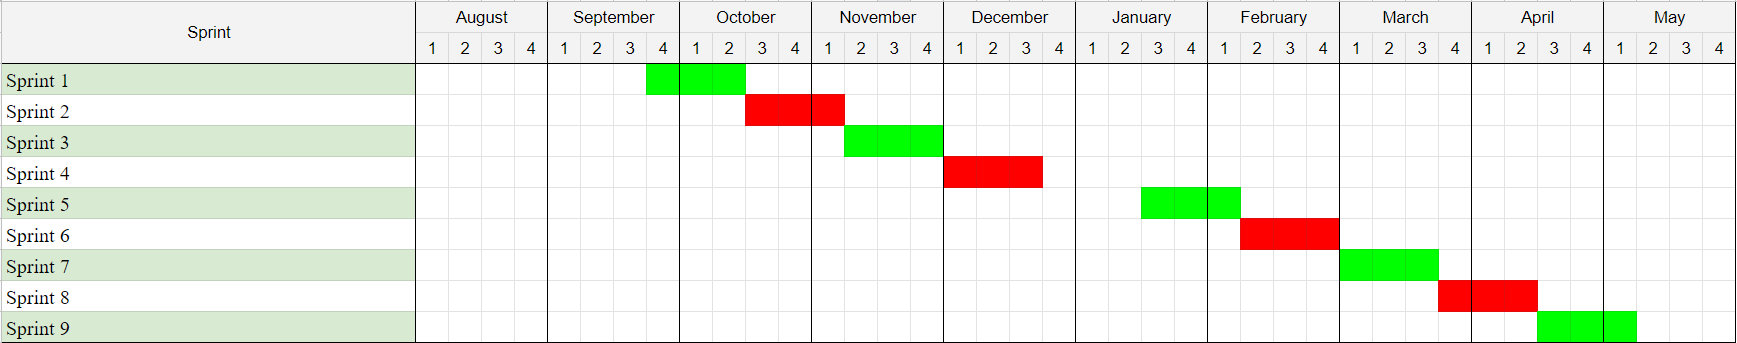
\includegraphics[width=16cm]{figure/intro-gantt-chart.png}
\captionof{figure}{Draft Schedule of the Project}
\label{fig:intro-gantt-chart}
\end{minipage}

\hspace{2em}The goal of the Sprints in the first semester focus on the design. The first Sprint is for research and designing the educational content. The second and the third Sprint are for designing the game systems. And the fourth, which is the last Sprint of the first semester focuses on finalizing the design and document.

\hspace{2em}The Sprints in the second semester focus on the implementation. The fifth Sprint is designated for prototyping. The sixth and the seventh Sprint are for developing each system in the game. The eighth Sprint is planned for integrating the game. And the ninth Sprint which is supposed to be the last is for testing the full game and finalizing the document of the project.

%%%%%%%%%%%%%%%%%%%%%%%%%%%%%%%%%%%%%%%%%%%%%%%%%%%%%%%%%%%%%%%%%%
%%%%%%%%%%%%%%  Literature Review %%%%%%%%%%%%%%%%%%%%%%%%%%%%%%%%%%%%%%%%%%%
%%%%%%%%%%%%%%%%%%%%%%%%%%%%%%%%%%%%%%%%%%%%%%%%%%%%%%%%%%%%%%%%%%
\chapter{Background Theory and Related Work}
\hspace{2em}For comprehension, we will present more information needed to understand our work. This chapter begins with theories involving game design, education design, and engineering content like the Genetic Algorithm. Then, we will describe the tools and technologies required to develop the game. Finally, we will discuss the works related to our project.

%\url{http://www.cpe.kmutt.ac.th}
%Explain theory, algorithms, protocols, or existing research works and tools related to your work. \cite{santi05b} \cite{bworld,hypersense}


%%%%%%%%%%%%%%%%%%%%%%%%%%%%%%%%%%%%%%%%%%%%%%%%%%%%%%%%%%%%%%%%%%
%%%%%%%%%%%%%%%%%%%%%%%%%%%%%%%%%%%%%%%%%%%%%%%%%%%%%%%%%%%%%%%%%%
\section{Game Design Theory}
This topic covers the game theories we used in this project including Natural Funativity, Maslow's Hierarchy of Needs, and Eight Kinds of ``Fun". We will apply these theories to increase the quality of our game in the aspect of ``Fun".

%%%%%%%%%%%%%%%%%%%%%%%%%%%%%%%%%%%%%%%%%%%%%%%%%%%%%%%%%%%%%%%%%%
\subsection{Natural Funativity}
According to Noah Falstein's theory \cite{steve2005introduction}, all fun derives from practicing survival and social skills, which consist of 3 categories.

\begin{enumerate}
	\item Physical Fun \\
	The fun of using the physical body which is strongly related to the survival instinct. Especially under depression or threatened situations which will instantly capture the attention. A game with intense and fast action like a first-person shooter (FPS) is a good example of a game introducing this type of fun. For playing such type of game, the player needs to observe the environment using their eyes, continuously control their in-game character using their hands, and act fast to fight the enemy to win the game.
	\item Social Fun \\
	The fun of interacting with others. The interaction can be conversations, competitions, cooperation, exchanges, etc. A multiplayer game like a massively multiplayer online role-playing game (MMORPG) is a good example of a game with social fun. In this type of game, the players continuously interact with other players in many ways through conversation, trading, or even competition. These activities sure give players a sense of social fun.
	\item Mental Fun \\
	The fun of using intelligence. It could be achieved in many ways, such as reasoning, planning, decision-making, recognizing, solving problems or puzzles, etc. The puzzle game, a game in which the players must continuously use their reasoning, planning, or problems solving skills to progress the game, is a perfect example of this type of fun.
\end{enumerate}

All the types of fun do not need to be all in a game to make it a fun game. But mixing more of these aspects of fun will help the game tend to be more fun and popular.

%%%%%%%%%%%%%%%%%%%%%%%%%%%%%%%%%%%%%%%%%%%%%%%%%%%%%%%%%%%%%%%%%%
\subsection{Maslow's Hierarchy of Needs}
Maslow's Hierarchy of Needs implies that one's motivation has an order to satisfy based on different needs \cite{saul2022simplypsychology}, representing each level in the Figure~\ref{fig:theory-maslow-needs} below.

\begin{figure}[!h]\centering
\fbox{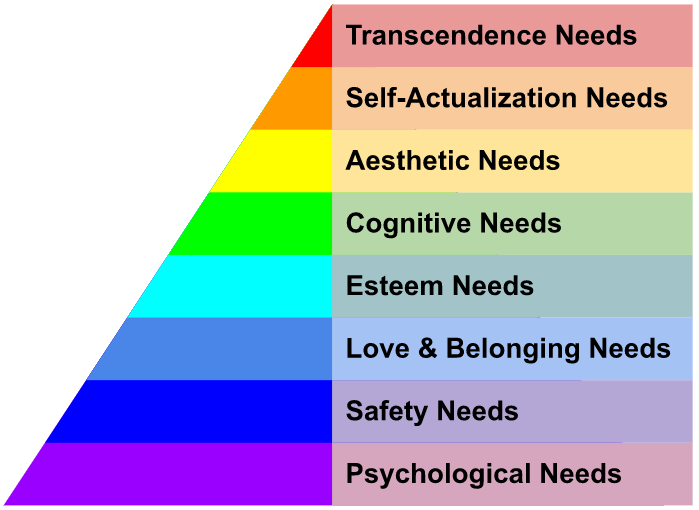
\includegraphics[width=8cm]{figure/theory-maslow-needs.png}}
\caption{Maslow's Hierarchy of Needs}
\label{fig:theory-maslow-needs}
\end{figure}

\begin{enumerate}
	\item Physiological Needs \\
	It is the most essential need for every human to survive, and it is mandatory to fulfill this kind of need before going further, such as air, water, food, clothing, etc. This level of need may be introduced as a health point system in a game that the player must maintain to survive.
	\item Safety Needs \\
	The need for stability in life, also regarded as the need for protection from threats, including personal security, shelter, order, law, etc. This level of need can be used as resources or items that the player could gather to make their character stronger and more stable.
	\item Love and Belonging Needs \\
	After the previous two needs have been fulfilled, the next level of need involves a social and a feeling of belongingness. Humans need to have a sense of unity with the environment. An example includes friendship, intimacy, trust, etc. The game applying this needs as a social system like co-op, guild, or multiplayer mode.
	\item Esteem Needs \\
	The esteem needs consist of two aspects, esteem for oneself and the desire for reputation or respect from others. This kind of need can be fulfilled by receiving dignity, achievement, status, prestige, etc. The achievement system of the game is a system directly derived from this level of needs.
	\item Cognitive Needs \\
	The need for learning, and gaining intelligence. This includes skill, knowledge, experience, understanding, curiosity, exploration, etc. The in-game character with a skill tree or an experience system is the application of this need.
	\item Aesthetic Needs \\
	This level of need is about seeking the thing that satisfies humans, as they need to search for and appreciate beauty, including balance, form, etc. The beautiful graphic of the game is also the aesthetic that fulfills this need of humans.
	\item Self-Actualization Needs \\
	This need is about realizing personal potential. Causing humans to need for personal growth, and trying to be everything one person could be. Creating an immersive game that drives the player to be in a way they have not experienced before is an example of fulfilling this need through the game.
	\item Transcendence Needs \\
	The ultimate need a person could wish. This level of need is motivated by values outside of self. This may be in a form of helping others or an ability to perform something mystical that a typical person can't do. The fantasy gameplay in which players can use magic; the famous player who helps other players in the game. These are examples of this need in the aspect of the game.
\end{enumerate}

%%%%%%%%%%%%%%%%%%%%%%%%%%%%%%%%%%%%%%%%%%%%%%%%%%%%%%%%%%%%%%%%%%
\subsection{Eight Kinds of “Fun”}
Marc LeBlanc proposed the idea of different kinds of “Fun” as a set of vocabularies to describe the kinds of fun that people are experiencing to be more specific and precise \cite{chris2016gnomestew}.

\begin{enumerate}
	\item Sensation - Game as sense-pleasure \\
	This kind of fun involves the physical senses of players, including visual, sound, sometimes physical movement, or even game pace.
	\item Fantasy - Game as make-believe \\
	It also acknowledged as escapism or immersion. It was gained by immersing oneself into the game world and possessing the ability to do things that cannot be done in the real world.
	\item Narrative - Game as drama \\
	It revolves around unfolding stories that the game has to offer. With narration, players get a sense of direction they can look forward to, sometimes even with their narration.
	\item Challenge - Game as obstacle course \\
	Overcoming courses of obstacles, solving difficult puzzles, defeating difficult enemies, or anything that provides highly competitive value to the player so they can challenge themselves.
	\item Fellowship - Game as social framework \\
	This kind of fun comes from gaining social interactions and cooperating with other players. A multiplayer game is a good example.
	\item Discovery - Game as uncharted territory \\
	Exploring new things in the game world or within oneself could be fun. Players could explore new area of maps, search for secret items, or dive through side stories.
	\item Expression - Game as self-discovery \\
	This kind of enjoyment comes from getting a chance to express oneself creatively, such as role-playing as a character in RPG games or conveying one's thoughts into creation in sandbox games.
	\item Submission - Game as pastime \\
	Doing daily tasks repetitively and playing the game casually, which are the opposite side of Challenge, also count as fun. Sometimes, just simply enjoying a game and relaxing are enough.
\end{enumerate}

%%%%%%%%%%%%%%%%%%%%%%%%%%%%%%%%%%%%%%%%%%%%%%%%%%%%%%%%%%%%%%%%%%
%%%%%%%%%%%%%%%%%%%%%%%%%%%%%%%%%%%%%%%%%%%%%%%%%%%%%%%%%%%%%%%%%%
\section{Education Design Theory}
This topic covers the education theories we used to design the education part of the game. We will apply these theories to ensure that our game will surely educate the player. Theories involved in this topic are Bloom's Taxonomy, Outcome-based Education, and the ADDIE model.

%%%%%%%%%%%%%%%%%%%%%%%%%%%%%%%%%%%%%%%%%%%%%%%%%%%%%%%%%%%%%%%%%%
\subsection{Bloom's Taxonomy}
The theory published by Benjamin Bloom presents the six levels of learning \cite{christine2021tophat}. These levels indicate the depth of learning and are used widely in the field of education. Each level of learning consists of a set of action verbs, the verb indicating whether the learner reaches the learning level. We use this theory to design the learning outcomes of the game.

\begin{figure}[!h]\centering
\fbox{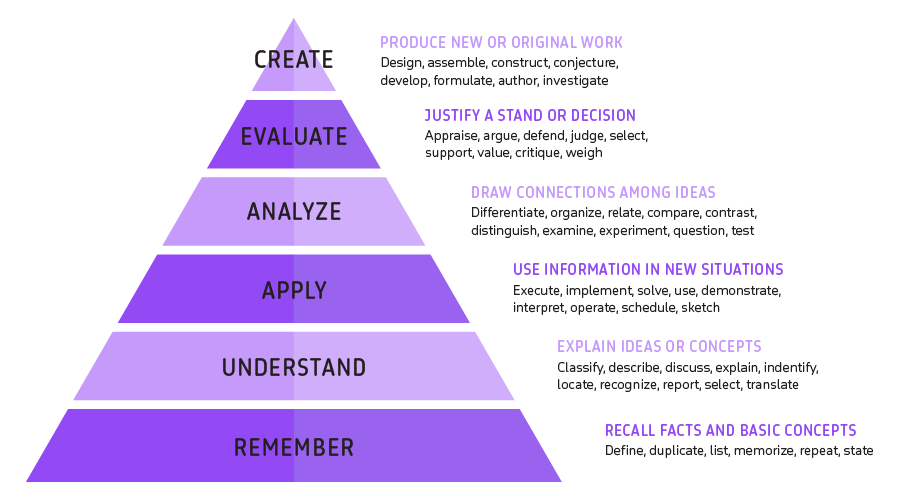
\includegraphics[width=14cm]{figure/theory-bloom.png}}
\caption[Bloom’s Taxonomy with Action Verbs]{Bloom’s Taxonomy with Action Verbs \cite{christine2021tophat}}
\label{fig:theory-bloom}
\end{figure}

Figure~\ref{fig:theory-bloom} shows all the learning levels and their action verbs. Each of them will be described below.

\begin{enumerate}
	\item Remember \\
	The lowest level of learning. The learner who achieves this level will be able to remember and recall the basic concepts of the knowledge. The action verbs in this level include duplicate, list, memorize, repeat, state, etc.
	\item Understand \\
	The learner is able to explain the concepts they have learned. The action verbs in this level include classify, demonstrate, explain, identify, illustrate, etc.
	\item Apply \\
	The learner is able to apply the knowledge to new situations they never met before. The action verbs in this level include implement, solve, use, operate, model, etc.
	\item Analyze \\
	The learner is able to compare the different knowledge and see connections among the ideas. The action verbs in this level include compare, contrast, distinguish, etc.
	\item Evaluate \\
	The learner is able to use the knowledge to judge the value of the idea and justify the decision. The action verbs in this level include appraise, judge, value, etc.
	\item Create \\
	The highest level of learning. The learner is able to assemble and produce a new work using the combination of previous knowledge. The action verbs in this level include build, develop, formulate, etc.
\end{enumerate}


%%%%%%%%%%%%%%%%%%%%%%%%%%%%%%%%%%%%%%%%%%%%%%%%%%%%%%%%%%%%%%%%%%
\subsection{Outcome-based Education}
Outcome-based education (OBE) is an education concept focusing on the learner's ability to perform the desired task at the end of the learning or outcome \cite{kmuttobe}. The curriculum is designed backward, starting from the outcome instead of what will be taught.

\begin{figure}[!h]\centering
\fbox{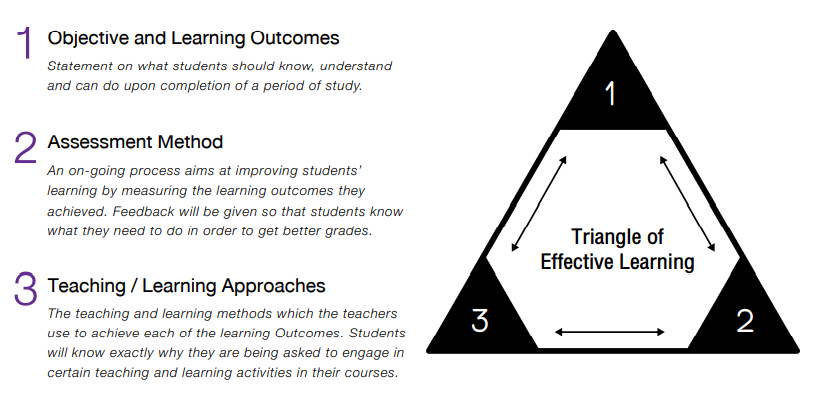
\includegraphics[width=14cm]{figure/theory-OBE.png}}
\caption[Triangle of Effective Learning]{Triangle of Effective Learning \cite{kmuttobe}}
\label{fig:theory-OBE}
\end{figure}

According to the triangle of Effective Learning in Figure~\ref{fig:theory-OBE}, the first step of designing is setting the learning outcome, which are skills we wish the learner to gain. The general format of the learning outcome is the action verb + object + qualifying phrase. An action verb can be derived from Bloom's taxonomy. A good learning outcome should match the SMART(TT) characteristics \cite{reginelo}, which is an abbreviation for

\begin{itemize}
	\item Speak to the learner: The outcome should specify what the learner will be able to do.
	\item Measurable: The outcome indicates how it will be assessed.
	\item Applicable: The outcome addresses the way the learner uses the gained skill.
	\item Realistic: The learner should be able to demonstrate the skill addressed in the outcome.
	\item Time-bound: The outcome should set the specific duration of the learning.
	\item Transparent: The learner can easily understand the outcome.
	\item Transferable: The skill in the outcome could be used in a wide range of contexts.
\end{itemize}

After the learning outcome is specified, design the assessment method to measure the learner's ability. The assessment criteria or a rubric must be specified. There is no need for one outcome to consist of only one benchmark. A good rubric should be observable and measurable.

Finally, the teaching and learning activities are designed based on learning outcomes and assessments. This includes not only the materials but also the activities. We adopt this concept in our educational game design in the education parts.

%%%%%%%%%%%%%%%%%%%%%%%%%%%%%%%%%%%%%%%%%%%%%%%%%%%%%%%%%%%%%%%%%%
\subsection{ADDIE Model}
ADDIE model is a model for designing and developing processes used widely in many fields, including education \cite{isfetaddie}. The model provides a systematic approach to the work process consisting of analysis, design, development, implementation, and evaluation, respectively. We apply the process of this model as the process for doing the project.

\begin{figure}[!h]\centering
\fbox{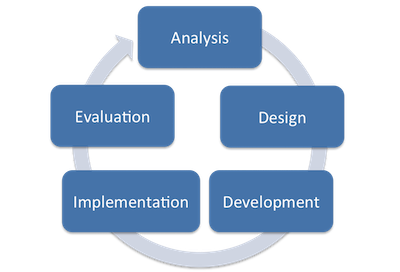
\includegraphics[width=7cm]{figure/theory-ADDIE.png}}
\caption[The phrases of the ADDIE Model]{The phrases of the ADDIE Model \cite{isfetaddie}}
\label{fig:theory-ADDIE}
\end{figure}

\begin{enumerate}
	\item Analysis \\
	The first step in the process focuses on identifying the problem, the learning environment, and the deliveries.
	\item Design \\
	The main task of this phase is defining the learning objectives, evaluation tools, and content development to suit the analyzed problem.
	\item Development \\
	After the design, the next step is developing the learning resources, including the learning material and learning activities. Those contents can be used later for the pilot test, a small-scale educational simulation used for gathering data about the feasibility of the project \cite{michiganpilot}. Such a test is applied to the group of target students to collect the necessary feedback for content revising.
	\item Implementation \\
	This step focuses on preparing the people involved in education and implementing the actual learning resources, such as content, material, and tool that have already been analyzed and designed. In the aspect of educational games, the main task of this step can be implementing the actual computer game software.
	\item Evaluation \\
	The last step of the model is an evaluation. The two methods of evaluation are formative evaluation and summative evaluation. Formative evaluation is the type of evaluation that is conducted at every stage of the ADDIE model and focuses on ongoing project revision. Summative evaluation occurs after the implementation, aiming to assert the learner's outcome and the effectiveness of the educational program once the course is completed.
\end{enumerate}


%%%%%%%%%%%%%%%%%%%%%%%%%%%%%%%%%%%%%%%%%%%%%%%%%%%%%%%%%%%%%%%%%%
%%%%%%%%%%%%%%%%%%%%%%%%%%%%%%%%%%%%%%%%%%%%%%%%%%%%%%%%%%%%%%%%%%
\section{Genetic Algorithm}
The Genetic Algorithm is the computer algorithm adapted from the Darwinian theory of Natural Selection \cite{immanuel2019genetic}. The algorithm introduces an easy-to-understand way to solve complicated problems since it's a technique with very little mathematics. Even deadlocked problems, the complex problems with conflicting conditions that require simultaneous solutions previously considered difficult can be solved with Genetic Algorithm \cite{man1996genetic}.

\begin{figure}[!h]\centering
\fbox{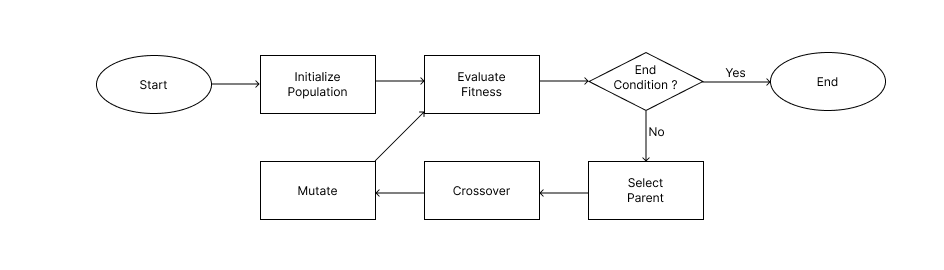
\includegraphics[width=14cm]{figure/theory-GA-flowchart.png}}
\caption{Flow Chart of Genetic Algorithm}
\label{fig:theory-GA-flowchart}
\end{figure}

The algorithm begins with encoding the possible solutions to the problem into a data structure called a chromosome. Such data structure usually is an array of bit values, the value that can be only 0 or 1. Other forms of data structure can be similarly used, for example, the matrix of the integer. Once the chromosome population is generated, they will be repeatedly evolved through the biological-inspired processes as shown in Figure~\ref{fig:theory-GA-flowchart}. Commonly, the Genetic Algorithm is used to generate the optimal solutions, the best solution among a vast number of generated possible solutions, for optimization and search problems. The detail of each process in the algorithm is described as follows.

%%%%%%%%%%%%%%%%%%%%%%%%%%%%%%%%%%%%%%%%%%%%%%%%%%%%%%%%%%%%%%%%%%
\subsection{Population Initialization}
Usually, the population initialization will be done via randomizing the set of valid possible solution chromosomes, the chromosomes that satisfy all the constraints. The population size must be large enough to maintain the diversity of the solution; otherwise, it will not be able to reach the global optimum solution in the end.

%%%%%%%%%%%%%%%%%%%%%%%%%%%%%%%%%%%%%%%%%%%%%%%%%%%%%%%%%%%%%%%%%%
\subsection{Fitness Evaluation}
	The fitness of a chromosome will be evaluated using specific methods, including fitness function and constraint. In a more general context, the fitness function is an objective function of an optimization problem which is a function that calculates the value we wish to maximize or minimize. In the context of the Genetic Algorithm, the fitness function is used to calculate the fitness value that indicates how close to the optimum solution of the chromosome is. If any chromosome violates the constraint, it is considered an invalid solution, and the fitness value of that chromosome will be zero.   \\
	In the Natural Selection rule, the survivor is one with the fittest properties. The chromosome with a higher fitness value tends to ``survive", selected by the algorithm during the parent selection process. The selected parent will inherit part of its chromosome to the offspring in the next generation through the crossover process. Meanwhile, the chromosome with lower fitness is likely to be destroyed.


%%%%%%%%%%%%%%%%%%%%%%%%%%%%%%%%%%%%%%%%%%%%%%%%%%%%%%%%%%%%%%%%%%.
\subsection{Genetic Operations}
The population will be evolved by generating a new population of the existing ones through genetic operations consisting of selection, crossover, and mutation.
\begin{itemize}
	\item Selection \\
	The subset of chromosomes will be selected from the current population as a parent for the next generation based on the fitness value. There are several basic ways to choose the parent, including random selection, tournament-based selection, roulette wheel selection, and ranked-based selection. Apart from the parent selection, there is also a technique that improves the algorithm called Elitism.
	\begin{enumerate}
		\item Random Selection \\
		This is the most straightforward method, which is a uniformly random selection of a chromosome out of the population. The probability of being selected is not related to the fitness value of an individual chromosome.
		\item Tournament-based Selection \\
		This method begins by randomly dividing the population into equal groups with the number of $K$ chromosomes in each group. Then, the chromosome with the best fitness value will be selected from each group. For example in Figure~\ref{fig:theory-GA-TBS}, the chromosomes are first picked as a group of 3, and the chromosome ``A'' is selected from the group due to its highest fitness value.
		
		\begin{minipage}[c]{\textwidth}\centering
		\fbox{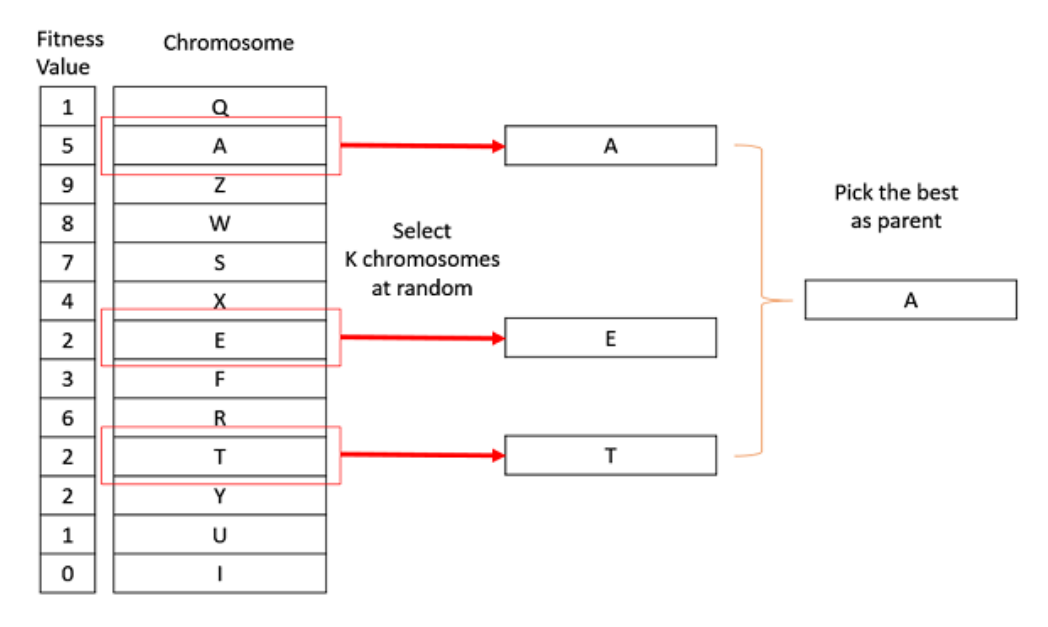
\includegraphics[width=10cm]{figure/theory-GA-TBS.png}}
		\captionof{figure}[Tournament-based Selection]{Tournament-based Selection \cite{immanuel2019genetic}}
		\label{fig:theory-GA-TBS}
		\end{minipage}

		\item Roulette Wheel Selection \\
		The method is based on proportionate randomization. It can be interpreted as a Roulette Wheel where each slot represents the chance of an individual chromosome to be chosen. As the chance of a chromosome being selected proportionate to its fitness. The higher fitness of the chromosome, the larger space on the wheel.

		\begin{minipage}[c]{\textwidth}\centering
		\fbox{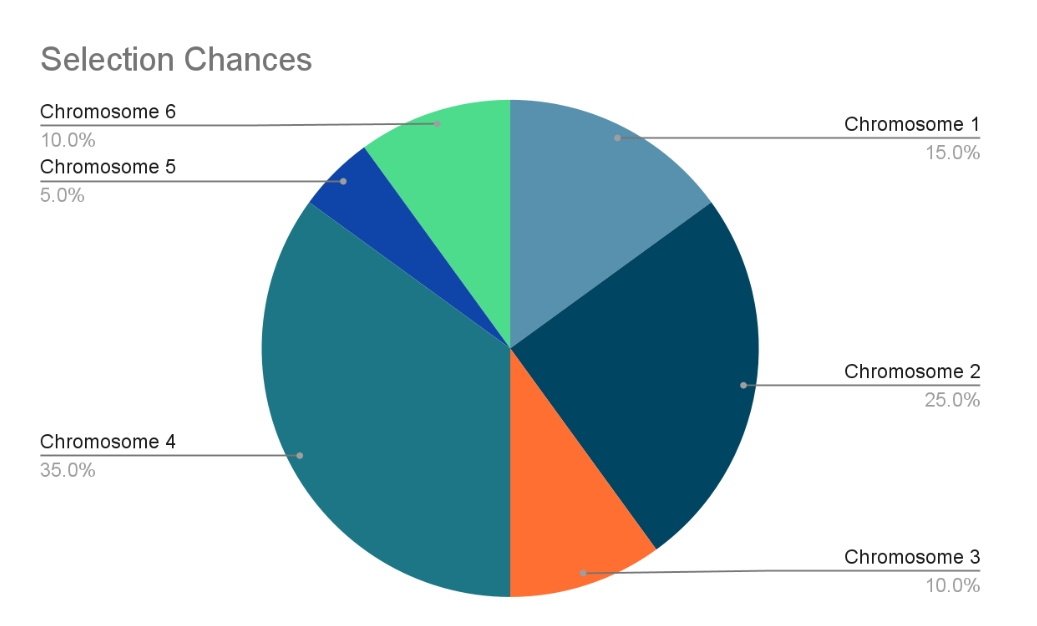
\includegraphics[width=10cm]{figure/theory-GA-RWS.png}}
		\captionof{figure}{Roulette Wheel Selection}
		\label{fig:theory-GA-RWS}
		\end{minipage}

		The selection chance for each chromosome is calculated using its fitness value divided by the total fitness value of all chromosomes in the population. In Figure~\ref{fig:theory-GA-RWS}, given that chromosome 4 has a fitness value of 7 and the total fitness value among the population is 20. So, the selection chance of chromosome 4 will be 7 divided by 20 which is equal to 0.35, or 35 percent.

		\item Rank-based Selection \\
		The selection method is based on the rank of the chromosome. The individual in the population is ranked according to their fitness value first. Then, assign a probability to be selected proportional to the individual rank. This can be done by reassigning the fitness value of the chromosome using the reversed rank. The worst chromosome will have fitness 1, the second worst will have fitness 2, and so on \cite{nidhi201comparative}. The best chromosome will have the highest fitness equal to the number of chromosomes in the population. \\

% Please add the following required packages to your document preamble:
% \usepackage{longtable}
% Note: It may be necessary to compile the document several times to get a multi-page table to line up properly
\begin{longtable}{|l|l|l|}
\caption{The Comparison Between Selection Methods.}
\label{tbl:selection-compare}\\
\hline
\multicolumn{1}{|c|}{Selection Method} &
  \multicolumn{1}{c|}{Advantage} &
  \multicolumn{1}{c|}{Disadvantage} \\ \hline
\endhead
%
Random &
  \begin{tabular}[c]{@{}l@{}}It is easy to understand \\ and implement.\end{tabular} &
  \begin{tabular}[c]{@{}l@{}}There is no use in the fitness value; \\ the good solution might be \\ accidentally destroyed.\end{tabular} \\ \hline
Tournament-based &
  \begin{tabular}[c]{@{}l@{}}It can be implemented \\ efficiently since no extra \\ calculation like a sorting\\ is required.\end{tabular} &
  \begin{tabular}[c]{@{}l@{}}If the tournament group is large, \\ the weak chromosome will have \\ a smaller chance to be selected.\end{tabular} \\ \hline
Roulette Wheel &
  \begin{tabular}[c]{@{}l@{}}The chromosome with \\ higher fitness has more \\ chance to be selected.\end{tabular} &
  \begin{tabular}[c]{@{}l@{}}It's not fair because the worst \\ chromosome will barely be \\ selected.\end{tabular} \\ \hline
Rank-based &
  \begin{tabular}[c]{@{}l@{}}All chromosomes have \\ a similar chance to be \\ selected which means \\ it preserves diversity.\end{tabular} &
  \begin{tabular}[c]{@{}l@{}}Computationally expensive \\ due to the sorting process. \\ The best solution is found slower \\ since the difference between \\ each chromosome is small.\end{tabular} \\ \hline
\end{longtable}

		All the parent selection methods have their advantages and disadvantages. The comparison between these methods \cite{nidhi201comparative} is discussed in Table ~\ref{tbl:selection-compare}.

		\item Elitism \\
		Elitism is a method that helps preserve the elites, some set of chromosomes with the highest fitness value, across the generations without any change. It improves the performance of the algorithm by ensuring the preservation of the best solution. However, increasing the ratio of the elites too much hurt the algorithm due to decreasing in population diversity. From the experiment, the algorithm with a higher reliability requirement needs a higher population size but lower elitism rate \cite{koljonen2006effects}. So, the elitism rate is preferred to be a small percentage value around 5\% to 10\% \cite{vinicius2022elitism}.
	\end{enumerate}
	\item Crossover \\
	The crossover is the process where a pair of selected parent chromosomes exchanges part of their information to produce a new pair of offspring. There are several basic ways to perform the crossover, including one-point crossover, two-point and k-point crossover, uniform crossover, and partially-mapped crossover (PMX).

	\begin{enumerate}
		\item Single-point Crossover \\
		The process of this type of crossover is illustrated in Figure ~\ref{fig:theory-GA-SPC}. The process begins with randomly selecting a single point on both parents' chromosomes as a crossover point. Then, the gene information from the right side of that point is exchanged with the other parent. The result is the pair of offspring chromosomes that inherit the gene information from both parents. This is one of the most simple crossover methods and it is also one of the lowest computational cost methods.

		\begin{minipage}[c]{\textwidth}\centering
		\fbox{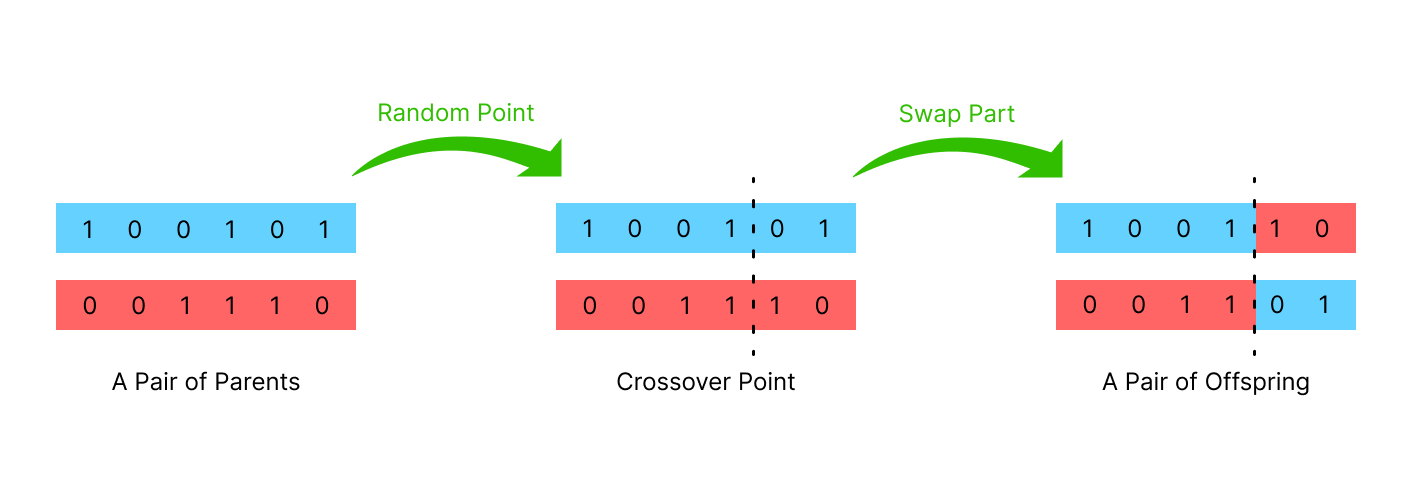
\includegraphics[width=10cm]{figure/theory-GA-SPC.png}}
		\captionof{figure}{Single-point Crossover}
		\label{fig:theory-GA-SPC}
		\end{minipage}

		\item Two-point and K-point Crossover \\
		The process of the two-point crossover and the k-point crossover is the same. The only difference between them is the number of crossover points. Figure~\ref{fig:theory-GA-TPC} shows the processes of the two-point crossover. Two points from both parents' chromosomes are randomly selected to be crossover points, dividing the chromosome into 3 sections. Then, the gene information in the second section (from left to right) which lay between these two points and is swapped between the parents to create two new offspring. Note that the first and the third sections of the chromosomes which are odd-numbered sections stay still.

		\begin{minipage}[c]{\textwidth}\centering
		\fbox{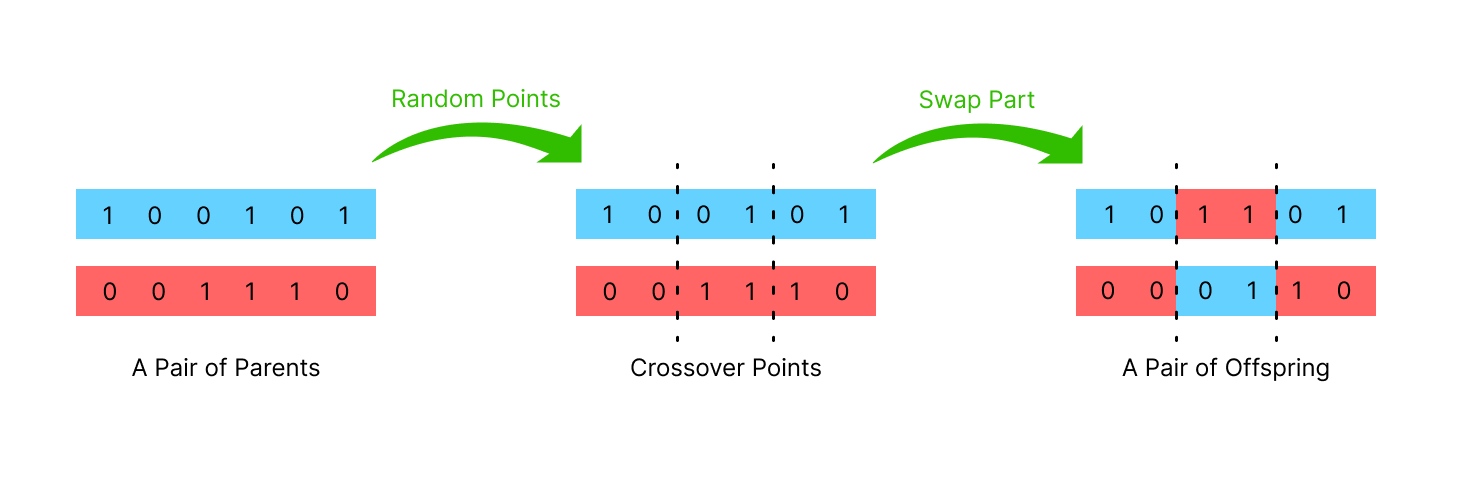
\includegraphics[width=10cm]{figure/theory-GA-TPC.png}}
		\captionof{figure}{Two-point Crossover}
		\label{fig:theory-GA-TPC}
		\end{minipage}

		For the k-point crossover, the $k$ crossover points are randomized, divide the chromosomes into $k+1$ sections. Same as the two-point crossover, the odd-numbered sections stay still. In the other hand, the even-numbered sections swapping between parents. This type of crossover help the chromosome be able to exchange its subset of information for multiple times.

		\item Uniform Crossover \\
		In this type, as shown in Figure~\ref{fig:theory-GA-UC}, the offspring are created by randomly swapping every piece of information in the parent' chromosome. The chance of switching each point is independent of another. This type of crossover allows the offspring to inherit from both parents equally and independently.

		\begin{minipage}[c]{\textwidth}\centering
		\fbox{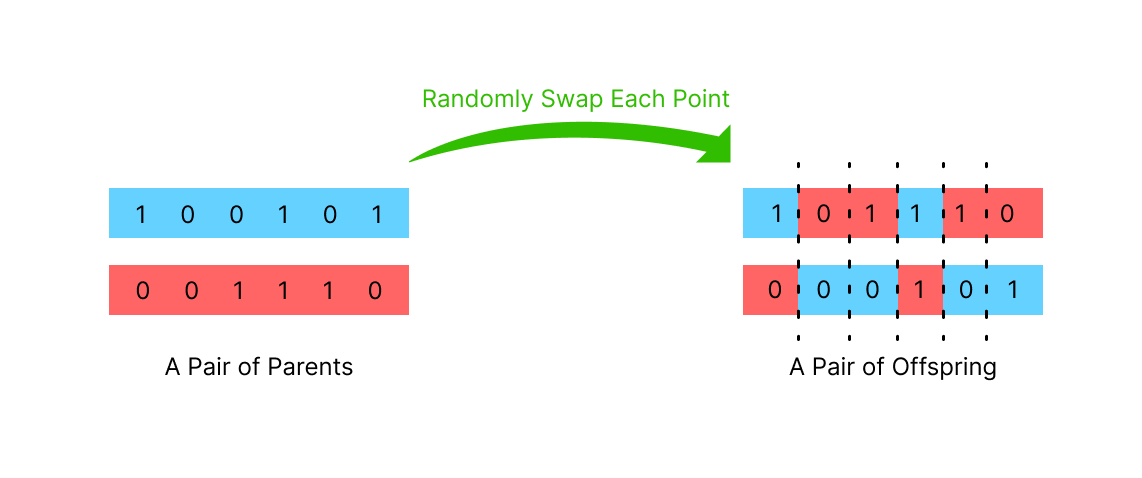
\includegraphics[width=10cm]{figure/theory-GA-UC.png}}
		\captionof{figure}{Uniform Crossover}
		\label{fig:theory-GA-UC}
		\end{minipage}

		\item Partially-Mapped Crossover (PMX) \\
		Whereas other previous methods cannot be implemented on the chromosome that can contain a duplicate value, the PMX can. To be accurate, PMX is a crossover method that only is used with the chromosome with such a condition. The method begins with randomly selecting two crossover points and swapping the chromosome information in the middle section. The swapped section is also called the mapping section since each information point on the parent is mapped with the corresponding point on another parent. Figure~\ref{fig:theory-GA-PMX1} shows an example of such mapping.

		\begin{minipage}[c]{\textwidth}\centering
		\fbox{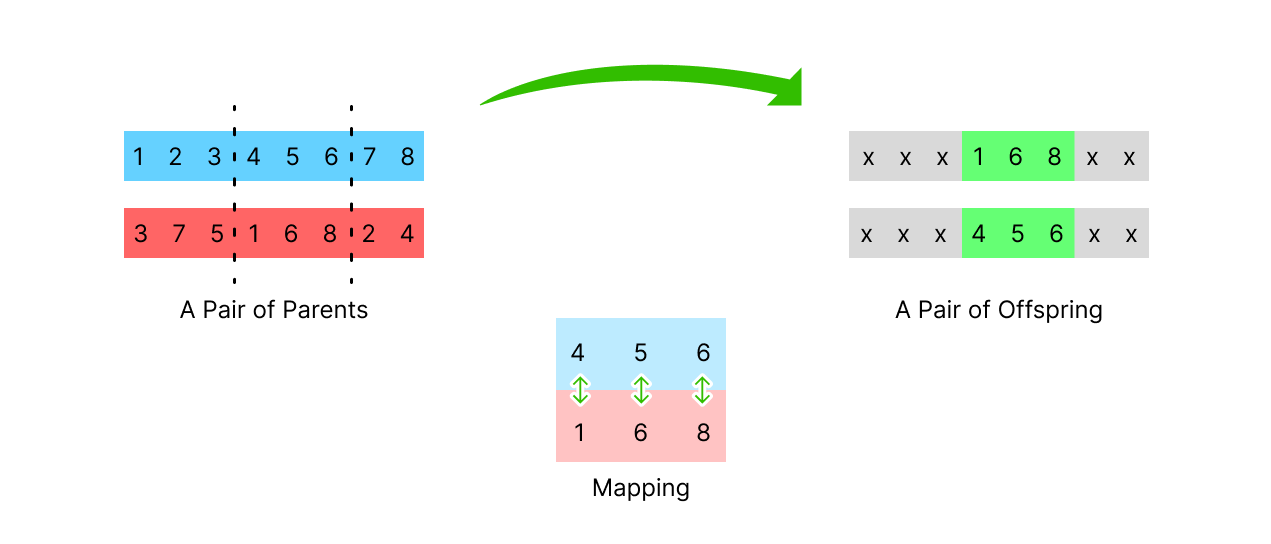
\includegraphics[width=10cm]{figure/theory-GA-PMX1.png}}
		\captionof{figure}{Mapping section of PMX}
		\label{fig:theory-GA-PMX1}
		\end{minipage}

		Then the information from its parent in the same position transfer to the offspring. If such information already exists in the offspring, that information will be changed into the corresponding value in the mapping until it turns out to be information that never exists in the offspring. In Figure~\ref{fig:theory-GA-PMX2}, the value 1 already exists in the offspring. So, it is changed into its mapping value which is 4.

		\begin{minipage}[c]{\textwidth}\centering
		\fbox{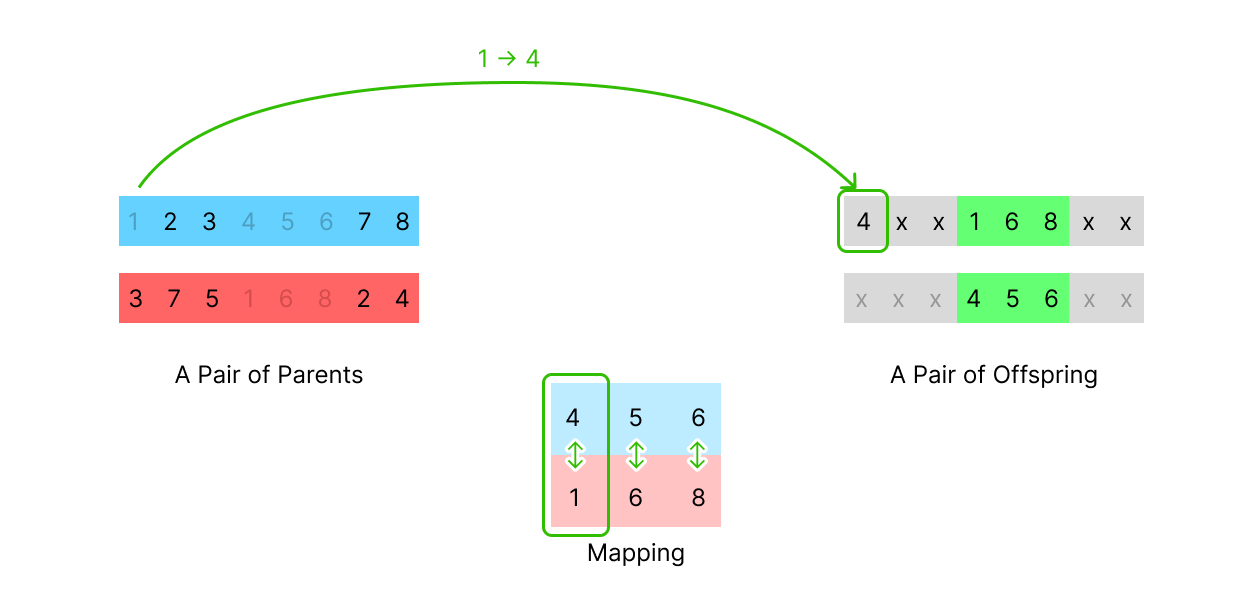
\includegraphics[width=10cm]{figure/theory-GA-PMX2.png}}
		\captionof{figure}{Mapping results in PMX}
		\label{fig:theory-GA-PMX2}
		\end{minipage}

		The rest of the information in both offspring is transferred in the same way. Figure~\ref{fig:theory-GA-PMX3} shows the final result of the PMX operation.

		\begin{minipage}[c]{\textwidth}\centering
		\fbox{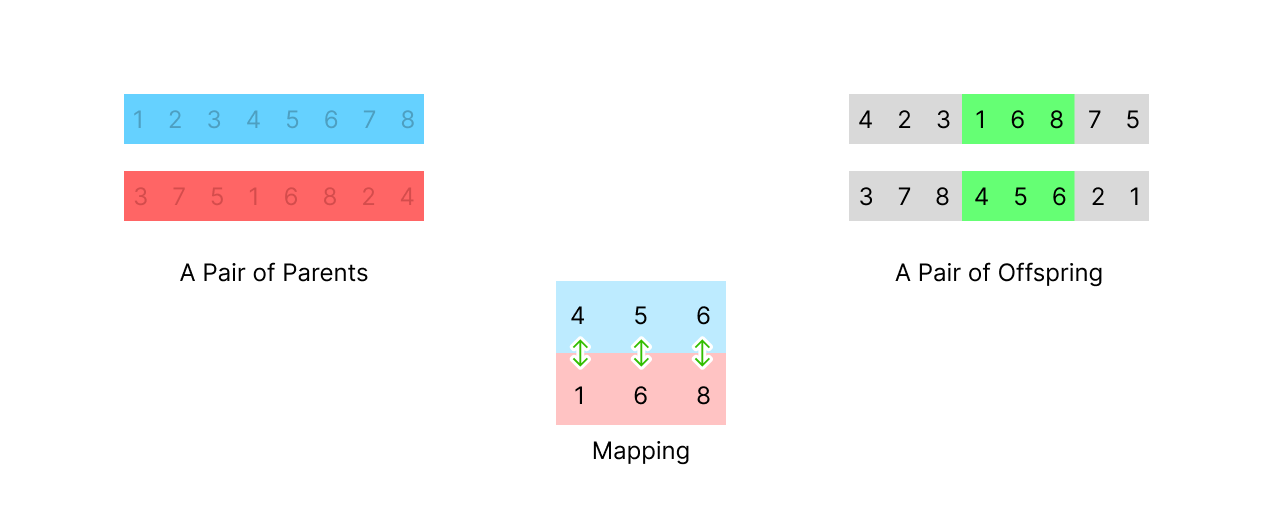
\includegraphics[width=10cm]{figure/theory-GA-PMX3.png}}
		\captionof{figure}{The final result of PMX}
		\label{fig:theory-GA-PMX3}
		\end{minipage}

	\end{enumerate}
	\item Mutation \\
	A mutation is a technique of altering the gene information of an individual chromosome. The procedure of altering the information varies and depends on how the solution is encoded. By performing this process, the chromosomes in a population can get better diversity. But just like Elitism, setting the mutation rate too high makes no good to the algorithm. If we use a high mutation rate, the algorithm would act as a random algorithm that does not utilize the advantage of using other genetic operations. So, the mutation rate is preferred to be a low value similar to the elitism rate. There are different types of basic mutation including bit flip mutation, flip bit mutation, and boundary mutation.
	\begin{enumerate}
		\item Bit Flip Mutation \\
		This type of mutation is used to alter the binary bit string chromosome, the chromosome consisting of only 0 and 1. The mutation can be done by randomly flipping the individual bit in the chromosome. The flipping of a bit can be done by changing its value from 0 to 1 or 1 to 0 depending on what the value it is before. For example in Figure~\ref{fig:theory-GA-bitflip}, the highlighted bit is changed from 0 to 1.

		\begin{minipage}[c]{\textwidth}\centering
		\fbox{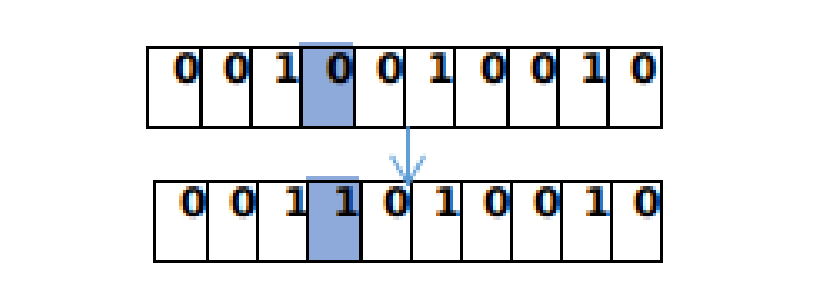
\includegraphics[width=5cm]{figure/theory-GA-bitflip.png}}
		\captionof{figure}[Bit Flip Mutation]{Bit Flip Mutation \cite{immanuel2019genetic}}
		\label{fig:theory-GA-bitflip}
		\end{minipage}

		\item Flip Bit Mutation \\
		This type of mutation is also used with the binary bit string chromosome. Performing this type of mutation, instead of flipping an individual bit in an individual chromosome, the whole chromosome is randomly selected and every bit within the chromosome will be flipped.
		\item Boundary Mutation \\
		This type of mutation suits the chromosome with an integer or float value. The process can be performed by replacing a specific value in the chromosome with the new random value of a lower or an upper range.

		% Please add the following required packages to your document preamble:
		% \usepackage{longtable}
		% Note: It may be necessary to compile the document several times to get a multi-page table to line up properly
		\begin{longtable}{|l|l|l|}
		\caption{The Comparison Between Mutation Methods}
		\label{tbl:mutation-compare}\\
		\hline
		\multicolumn{1}{|c|}{Mutation Method} &
		  \multicolumn{1}{c|}{Amount of Changed value} &
		  \multicolumn{1}{c|}{\begin{tabular}[c]{@{}c@{}}Suitable Type of \\ Chromosome\end{tabular}} \\ \hline
		\endhead
		%
		Bit Flip & \begin{tabular}[c]{@{}l@{}}Randomized individual \\ value within a chromosome\end{tabular} & Binary bit string \\ \hline
		Flip Bit & \begin{tabular}[c]{@{}l@{}}All information in \\ randomized chromosome\end{tabular}        & Binary bit string \\ \hline
		Boundary & \begin{tabular}[c]{@{}l@{}}Randomized individual \\ value within a chromosome\end{tabular} & Integer or float  \\ \hline
		\end{longtable}

		Each mutation method suits a different type of chromosome and changes a different amount of value. Table~\ref{tbl:mutation-compare} shows a brief comparison of each method.

	\end{enumerate}
\end{itemize}

%%%%%%%%%%%%%%%%%%%%%%%%%%%%%%%%%%%%%%%%%%%%%%%%%%%%%%%%%%%%%%%%%%
\subsection{Knapsack Problem}
The real-world problem involving our project is the knapsack problem and its variant, it's one of the most popular optimization problems that can be solved using Genetic Algorithm \cite{laabadi20180}. To be accurate, the problems include Standard 0/1 Multidimensional Knapsack Problem (MKP) and Multiple 0/1 Multidimensional Knapsack Problem. The word 0/1 indicates that the problem can be encoded as a binary bit string chromosome as the solution shown in \cite{arpit2022}. The setting and goal of each problem will be described below.

\begin{enumerate}
	\item Standard 0/1 MKP \\
	Generally, the standard knapsack problem is a problem that deals with packing items in a bag while maximizing the value of the bag. Each item has its weight and value, and the bag can hold some amount of maximum weight. This maximum weight can be interpreted as a constraint that the solution must follow. The solution is invalid when the total weight of the picked items exceeds the maximum weight of the bag. The word Multidimension indicates the dimension of the knapsack or the number of constraints. For example, the Standard 0/1 MKP that has only the constraint of the weight limit can be described as only 1 dimension knapsack. The binary bit string chromosome of length equal to the number of items can be used as a solution representation. Using this type of chromosome, the value of each bit indicates whether the item with the corresponding index is selected or not. \\

	\begin{minipage}[c]{\textwidth}\centering
	\fbox{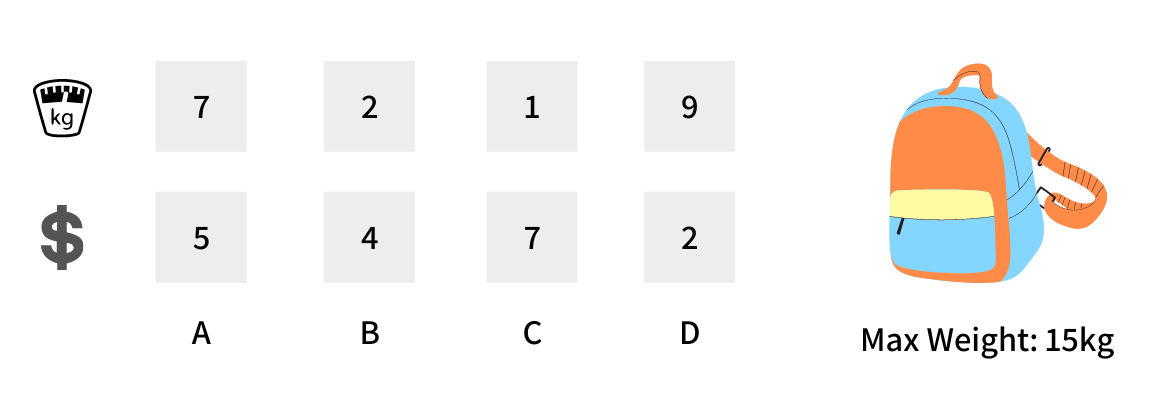
\includegraphics[width=10cm]{figure/theory-knapsack-setting.png}}
	\captionof{figure}[Example of Standard Knapsack Problem Setting]{Example of Standard Knapsack Problem Setting \cite{arpit2022}}
	\label{fig:theory-knapsack-setting}
	\end{minipage}	
	Figure~\ref{fig:theory-knapsack-setting} shows the example of Standard MKP. There are four items which are A, B, C, and D. Each item has a weight of 7, 2, 1, and 9; and has a value of 5, 4, 7, and 2 respectively. The constraint is that the knapsack can hold a maximum total weight equal to 15. \\

	\begin{minipage}[c]{\textwidth}\centering
	\fbox{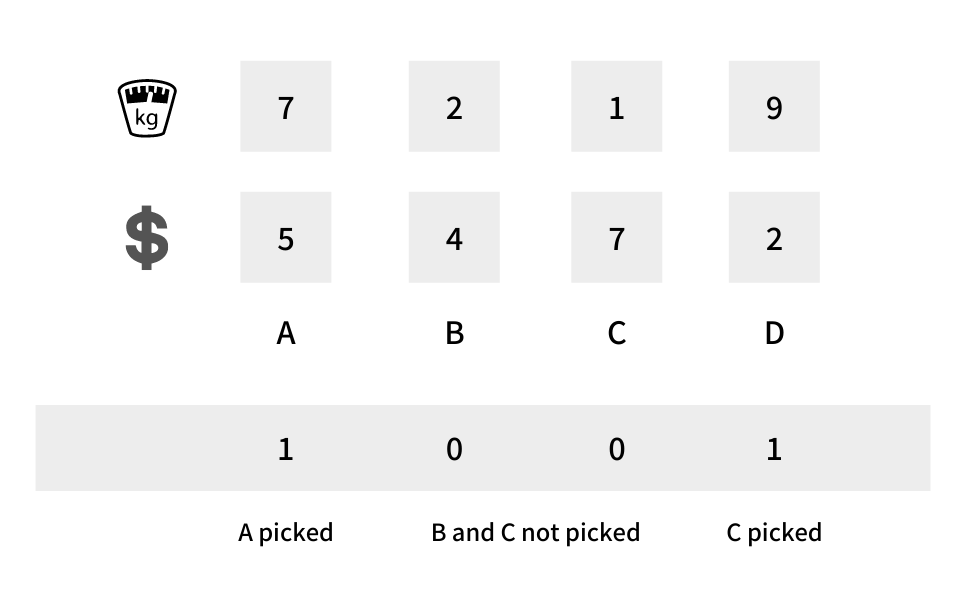
\includegraphics[width=10cm]{figure/theory-knapsack-chromosome.png}}
	\captionof{figure}[Example of Chromosome Representation of the Standard Knapsack Solution]{Example of Chromosome Representation of the Standard Knapsack Solution \cite{arpit2022}}
	\label{fig:theory-knapsack-chromosome}
	\end{minipage}
	Since there are four items, the binary bit string chromosome with a length of four can be used as an encoded representation of the solution. Figure~\ref{fig:theory-knapsack-chromosome} demonstrates the chromosome with the value of 1, 0, 0, and 1. By decoding these values, we get the solution which is picking items A and D into a knapsack. Using encoding and decoding this way, we can represent any solution using the binary bit string; and we can finally use a Genetic Algorithm to solve such a problem.\\

	\item Multiple 0/1 MKP \\
	The setting and the goal of the Multiple 0/1 MKP are similar to the Standard 0/1 MKP. The difference between them is the number of knapsacks in Multiple 0/1 MKP is more than one. The goal of this problem is not only the decision about whether a specific item is selected but also involves choosing the knapsack such an item should be in. The binary bit string chromosome of the length of the number of items (N) multiplied by the number of knapsacks (M) can be used as a solution representation. The first N bit in the chromosome indicates whether the item with the corresponding index is selected to be in the first knapsack or not. The next N bit of the chromosome is the indicator for the second knapsack and so on. The solution is also invalid if the same item is selected to be in more than a single knapsack.	
\end{enumerate}

%These are some problems that can be solved by using the genetic algorithm.
%
%\begin{enumerate}
%	\item Multivariable Equation \\
%	The Equation is a mathematical problem where we must find the value of unknown variables from the given conditions. For a single equation with multiple variables, there is no exact answer, and can't be solved deterministically. Since it can't be solved deterministically but it has a way to check whether the value of variables 	satisfies the equation, the genetic algorithm can be used \cite{tejaswee2020medium}.
%	\item Partition \\
%	The Partition problem is a special case of a subset sum problem which is a problem about dividing the existing set of numbers into many groups with the most similar summation \cite{Junkermeier2015AGA}. For the Partition problem, the existing numbers will be divided into 2 groups. The optimal solution to the problem is a division that 2 groups have an equal summation.
%	\item Knapsack \\
%	The Knapsack problem is a problem that deals with packing items in a bag while maximizing the value of the bag \cite{arpit2022}. Each item has its weight and value, and the bag can hold some amount of maximum weight. This maximum weight can be interpreted as a constraint that the solution must follow. The solution is invalid when the total weight of the picked items exceeds the maximum weight of the bag.
%	\item Graph Coloring \\
%	The Graph Coloring problem is a problem about coloring the node of the graph without constraint violation \cite{hindi2012genetic}. Such constraints are a condition that the connected nodes can't be the same color. The problem also could limit the maximum number of colors that can be used. The ultimate solution to the problem is graph coloring without any constraint violation with the minimum number of colors.
%	\item Traveling Salesman \\
%	The Traveling Salesman Problem (TSP) is a problem about a salesman finding a good route for traveling through the cities \cite{larranaga1999genetic}. For the single route TSP, the salesman must travel to every city, once per city. The goal of this problem is to find a route that has a minimum summation of distance.
%\end{enumerate}

%\section{Recommender Systems}
%
%\begin{table}[!h]
%\caption{test table method1}\label{tbl:method1}
%\begin{tabular}{c|c|l|rr} \hline\hline
%Center & Center & left aligned & Right & Right aligned \\ \hline\hline
%Center & Center & left aligned & Right & Right aligned \\ \hline
%Center & Center & left aligned & Right & Right aligned \\ 
%Center & Center & left aligned & Right & Right aligned \\ \hline
%Center & Center & left aligned & Right & Right aligned \\ \hline\hline
%\end{tabular}
%\end{table}


%\section{Text Processing Algorithms}
%\subsection{Algorithm I}
%
%
%% Can define this in the preamble..
%You can place the figure and refer to it as Figure~\ref{fig:model2}.
%The figure and table numbering will be run and updated automatically when you add/remove tables/figures from the document.
%
%\begin{figure}[!h]\centering
%\setlength{\fboxrule}{0.2mm} % can define this in the preamble
%\setlength{\fboxsep}{1cm}
%\fbox{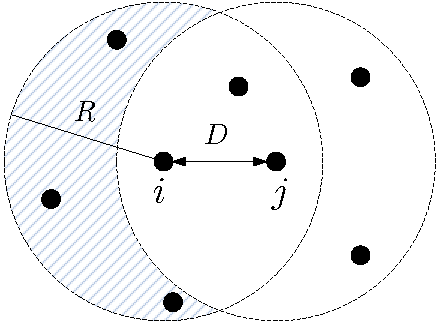
\includegraphics[width=5cm]{./model2.pdf}}
%\caption{The network model}\label{fig:model2}
%\end{figure}

%%%%%%%%%%%%%%%%%%%%%%%%%%%%%%%%%%%%%%%%%%%%%%%%%%%%%%%%%%%%%%%%%%
\section{Usability Testing}
\hspace{2em}Usability testing aims to understand how users interact with the product and find issues in existing products \cite{nick2021usability}. The information gathered from the test can be used to improve the design or current development. In general, the usability testing questions are divided into 3 sets which are screening, in-test and post-test.

\hspace{2em}The screening question indicates whether the participants represent the target group. The data from this type of question includes both demographic and personal experiences. The in-test question aims to find insight into user behaviors such as the reason behind the user's certain actions. The insight from this section usually be generated during the user's interaction with the product. The post-test question aims to gather the user's additional feedback. The opinion gathered from this section can be useful for product improvement.

\hspace{2em}With the reason for the benefit-cost ratio, the recommended test user size is 5 \cite{jakob2012usability}. With this size of the test user, almost all usability problems will be found while the effort of performing the test is not too high.

%%%%%%%%%%%%%%%%%%%%%%%%%%%%%%%%%%%%%%%%%%%%%%%%%%%%%%%%%%%%%%%%%%
\section{Languages and Technologies}
We will use multiple programs and platforms to complete this project, including Unity, the game engine of choice, visual studio, the code editor compatible with Unity, C\#, the programming language for Unity, GitHub, the version control platform, and Figma, for model creation.

\begin{enumerate}
	\item C\# \\
	C\# (pronounced "See Sharp") is one of programming languages used in many game engines including Unity.  It is a modern, object-oriented, and type-safe programming language based on the C family of languages similar to C, C++, Java, and JavaScript. It can be used for creating secure and robust  applications, with many useful features such as nullable types, exception handling, and lambda expressions to serve multiple purposes of programming.
	\item Unity \\
	Unity is a popular free game engine used to create both 3D and 2D games for multiple platforms; in 2020, 61\% of surveyed developers decided to use Unity as their preferred game engine \cite{unity2021}, and the number increase by 31\% in 2021 \cite{unity2022}. Unity may be described as Integrated Development Environment (IDE), providing several prominent features for creating games, such as physics, 3D rendering, collision detection, etc. Besides a simple drag-and-drop interface, Unity also provides a way to customize the game through C\# coding. Compared to the similarly popular game engine, Unreal Engine \cite{perforce2022}, Unity is considered more lightweight and beginner-friendly, with various platform integrations and dedicated tools for 2D game development \cite{ben2022}. Apart from said features and our previous experience with this game engine, we also chose Unity due to its popularity, which makes the community pretty huge and helps when we run into trouble while developing games.
	\item Visual Studio \\
	Visual Studio is the Integrated Development Environment (IDE) software for writing and editing code. It can work with various types of programming languages such as C\#, C++, Python, etc. It is one of the most popular IDE to work with Unity since it includes many extensions and powerful features to C\# programming.
	\item GitHub \\
	GitHub is a code hosting platform for version control and collaboration through git repositories. Users can edit codes without harming the main project by creating a new branch to work. After committing changes, a branch can be merged back to the main branch by creating a pull request to let other collaborators review the code before pulling it into the master branch.
	\item Figma \\
	Figma is a web-based app for designing and working with graphics. It has the ability to design all kinds of graphics, including websites, mobile app interfaces, prototyping designs, etc. The fact that Figma is available on multiple platforms containing various sets of designing tools available to use and collaboration features for team projects \cite{daniel2022} makes it to be one of the most widely-used graphic tools.
	\item Aseprite \\
	Aseprite is a pixel art tool for creating pixel art images and 2D animations. It offers various tools for creating 2D art, such as shading, pixel-perfect strokes, tiled mode, and filled and contour options. Additionally, it provides animation tools, including a real-time animation preview feature that helps users create pixel art or animation. It allows users to create multiple layers of art, separating the usage of layers for still images and frames for animations. This makes it easier to have art with multiple layers and create animations by specifying a specific layer in each frame.
\end{enumerate}


%%%%%%%%%%%%%%%%%%%%%%%%%%%%%%%%%%%%%%%%%%%%%%%%%%%%%%%%%%%%%%%%%%
%%%%%%%%%%%%%%%%%%%%%%%%%%%%%%%%%%%%%%%%%%%%%%%%%%%%%%%%%%%%%%%%%%
\section{Related Works}
These are some works and research relating to our project, which will be our reference.

%%%%%%%%%%%%%%%%%%%%%%%%%%%%%%%%%%%%%%%%%%%%%%%%%%%%%%%%%%%%%%%%%%
\subsection{Similar Games Genres}
Our game can be considered as various genres including visual novels, puzzles, and education.

\begin{enumerate}
	\item Visual Novel \\
	A Visual Novel (VN) is a game genre that mainly focuses on story narration through text with the help of static arts, sound effects, and soundtracks, similar to a graphic novel as per the name suggested \cite{camingue2021visualnovel}. Players can interact with the game by clicking or tapping to progress the story; this system is called On-Click Progression. Furthermore, the game may provide players with extra interactions, such as dialogue choices or actions that may affect the story.
	\item Puzzle Game \\
	A puzzle game is a problem that has a correct answer for players to discover \cite{zhang2019puzzle}. Players must understand the concepts and features of the game and apply those rules with one’s logical thinking to reach the goal. A good puzzle game should be entertaining and have an appropriate difficulty level for its target group.
	\item Educational Game \\
	An educational game is a type of game that integrates academic and training factors into its gameplay, story narration, and other elements \cite{dondlinger2007educational}. It requires players to use various skills such as problem-solving, strategizing, and other higher-order thinking skills in order to achieve goals and receive rewards.
\end{enumerate}

%%%%%%%%%%%%%%%%%%%%%%%%%%%%%%%%%%%%%%%%%%%%%%%%%%%%%%%%%%%%%%%%%%
\subsection{Similar Games Example}
There are many similar games to our final project, which can be used as references or ideas for other people to fortify the images of the project.

\begin{enumerate}
	\item Dragon City \\
	Dragon City is a free-to-play breeding simulator game developed and published by Social Point. This game lets players build a farm of dragons on floating islands, which players can breed and collect variances of dragons to battle with other players for rewards. Each dragon can be fed and evolve into a stronger dragon with many skills to learn. We decided to integrate their theme of collecting monsters and putting them on a farm into our game. \\
	Due to its multiplayer-based nature, players can communicate and group up with other players as a guild to share information and passion about the game with each other, enjoying their given social fun. They can also participate in competitions between players to climb to higher ranks, fulfilling their esteem needs. There are countless dragons for players to discover and collect, giving them discovery fun. \\
	\begin{minipage}[c]{\textwidth}\centering
	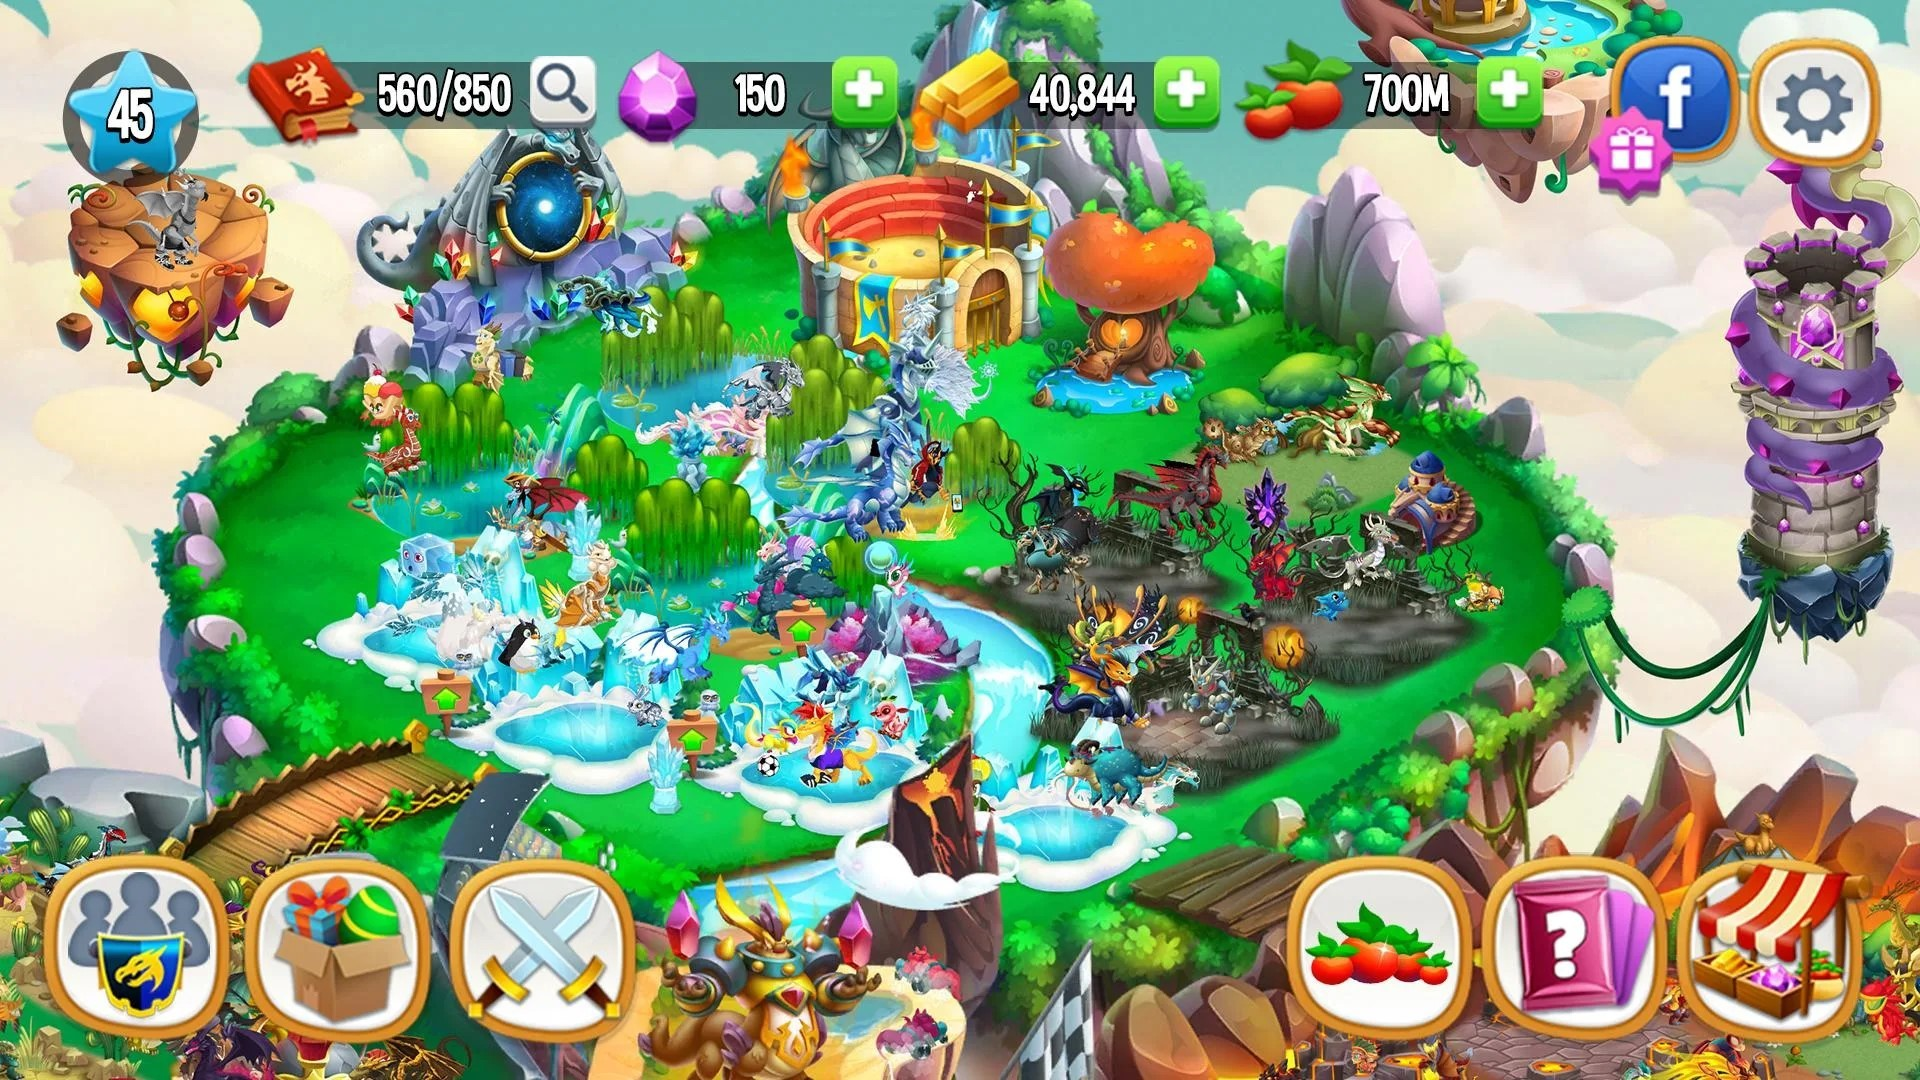
\includegraphics[width=8cm]{figure/related-work-dragon-city.png}
	\captionof{figure}[Game Example: Dragon City]{Game Example: Dragon City 
		\\ Source: \href{https://play.google.com/store/apps/details?id=es.socialpoint.DragonCity&hl=en_US&gl=US}{Google Play}}
	\label{fig:related-work-dragon-city}
	\end{minipage}

	\item Princess Connect! Re:Dive \\
	Princess Connect! Re:Dive (Priconne) is a free-to-play fantasy RPG game developed by Cygames. Players can build teams of characters they pulled from gacha and use them to clear dungeons and battle with other players. Characters can be categorized into multiple groups based on various classification, such as standing position (front, middle, back) or roles (tanker, attacker, supporter). During battle, characters will battle automatically with their preset moves, and players can use their ultimate move when the corresponding gauge is filled. We carefully extracted some of the arena elements into our game, more details will be covered in the next chapter. \\
	Similar to the previous game, this game has multiplayer features like the Guild system and PVP system for players to gain esteem needs, social fun, and fellowship fun. It also has tons of refined characters to collect. Moreover, there are multiple engaging voice-over stories with animations displayed as a visual novel during the story telling section, completing players' narrative fun. \\
%	\begin{minipage}[c]{\textwidth}\centering
%	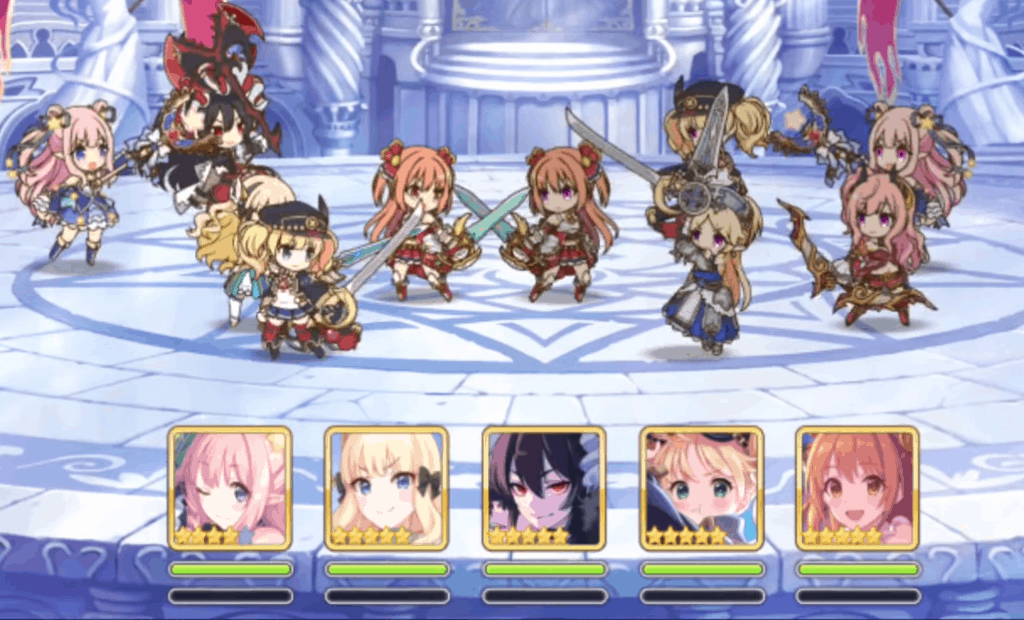
\includegraphics[width=8cm]{figure/related-work-princon.png}
%	\captionof{figure}[Game Example: Princess Connect! Re:Dive]{Game Example: Princess Connect! Re:Dive 
%		\\ Source: \href{https://gachafix.com/is-princess-connect-good/}{gachafix.com}}
%	\label{fig:related-work-princon}
%	\end{minipage}

    	\captionsetup{justification=centering}	
	\begin{minipage}[c]{\textwidth}\centering
	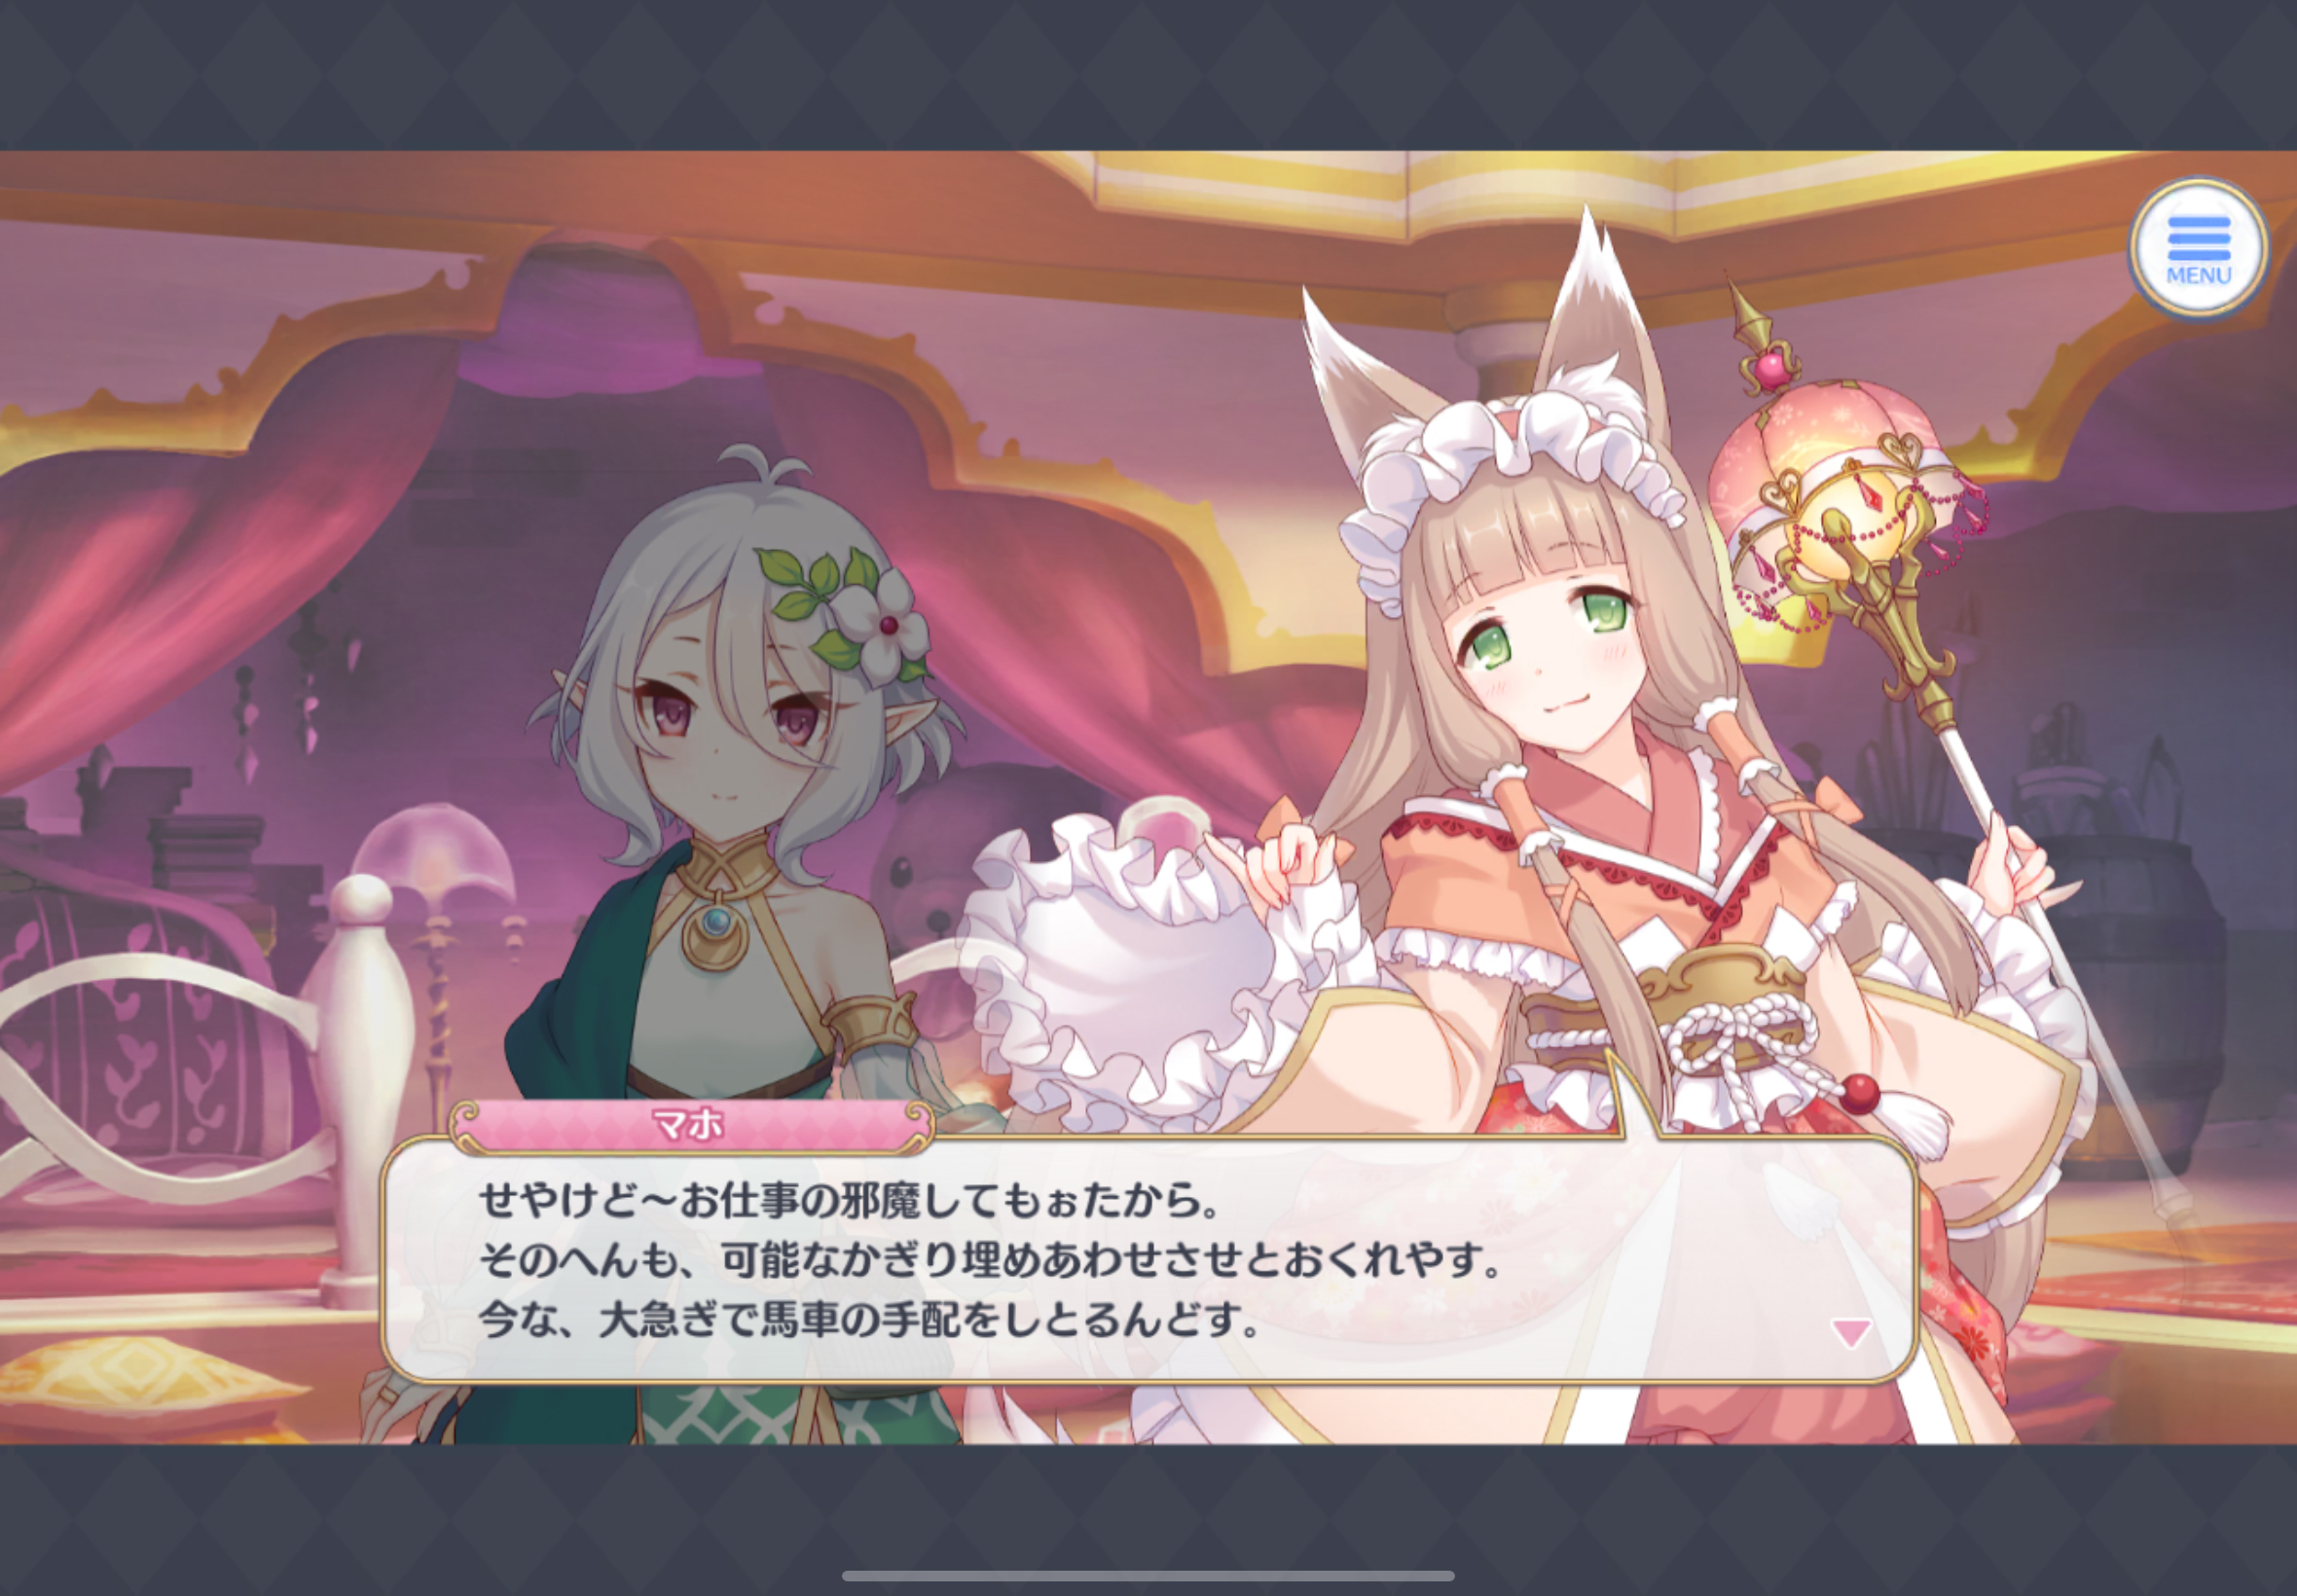
\includegraphics[width=8cm]{figure/related-work-princon-story.png}
	\captionof{figure}[Game Example: Princess Connect! Re:Dive (Story Section)]{Game Example: Princess Connect! Re:Dive (Story Section)
		\\ Source: Cygames Inc. (2023). Princess Connect! Re:Dive. Screenshot by Author.}
	\label{fig:related-work-princon-story}
	\end{minipage}
	
	\begin{minipage}[c]{\textwidth}\centering
	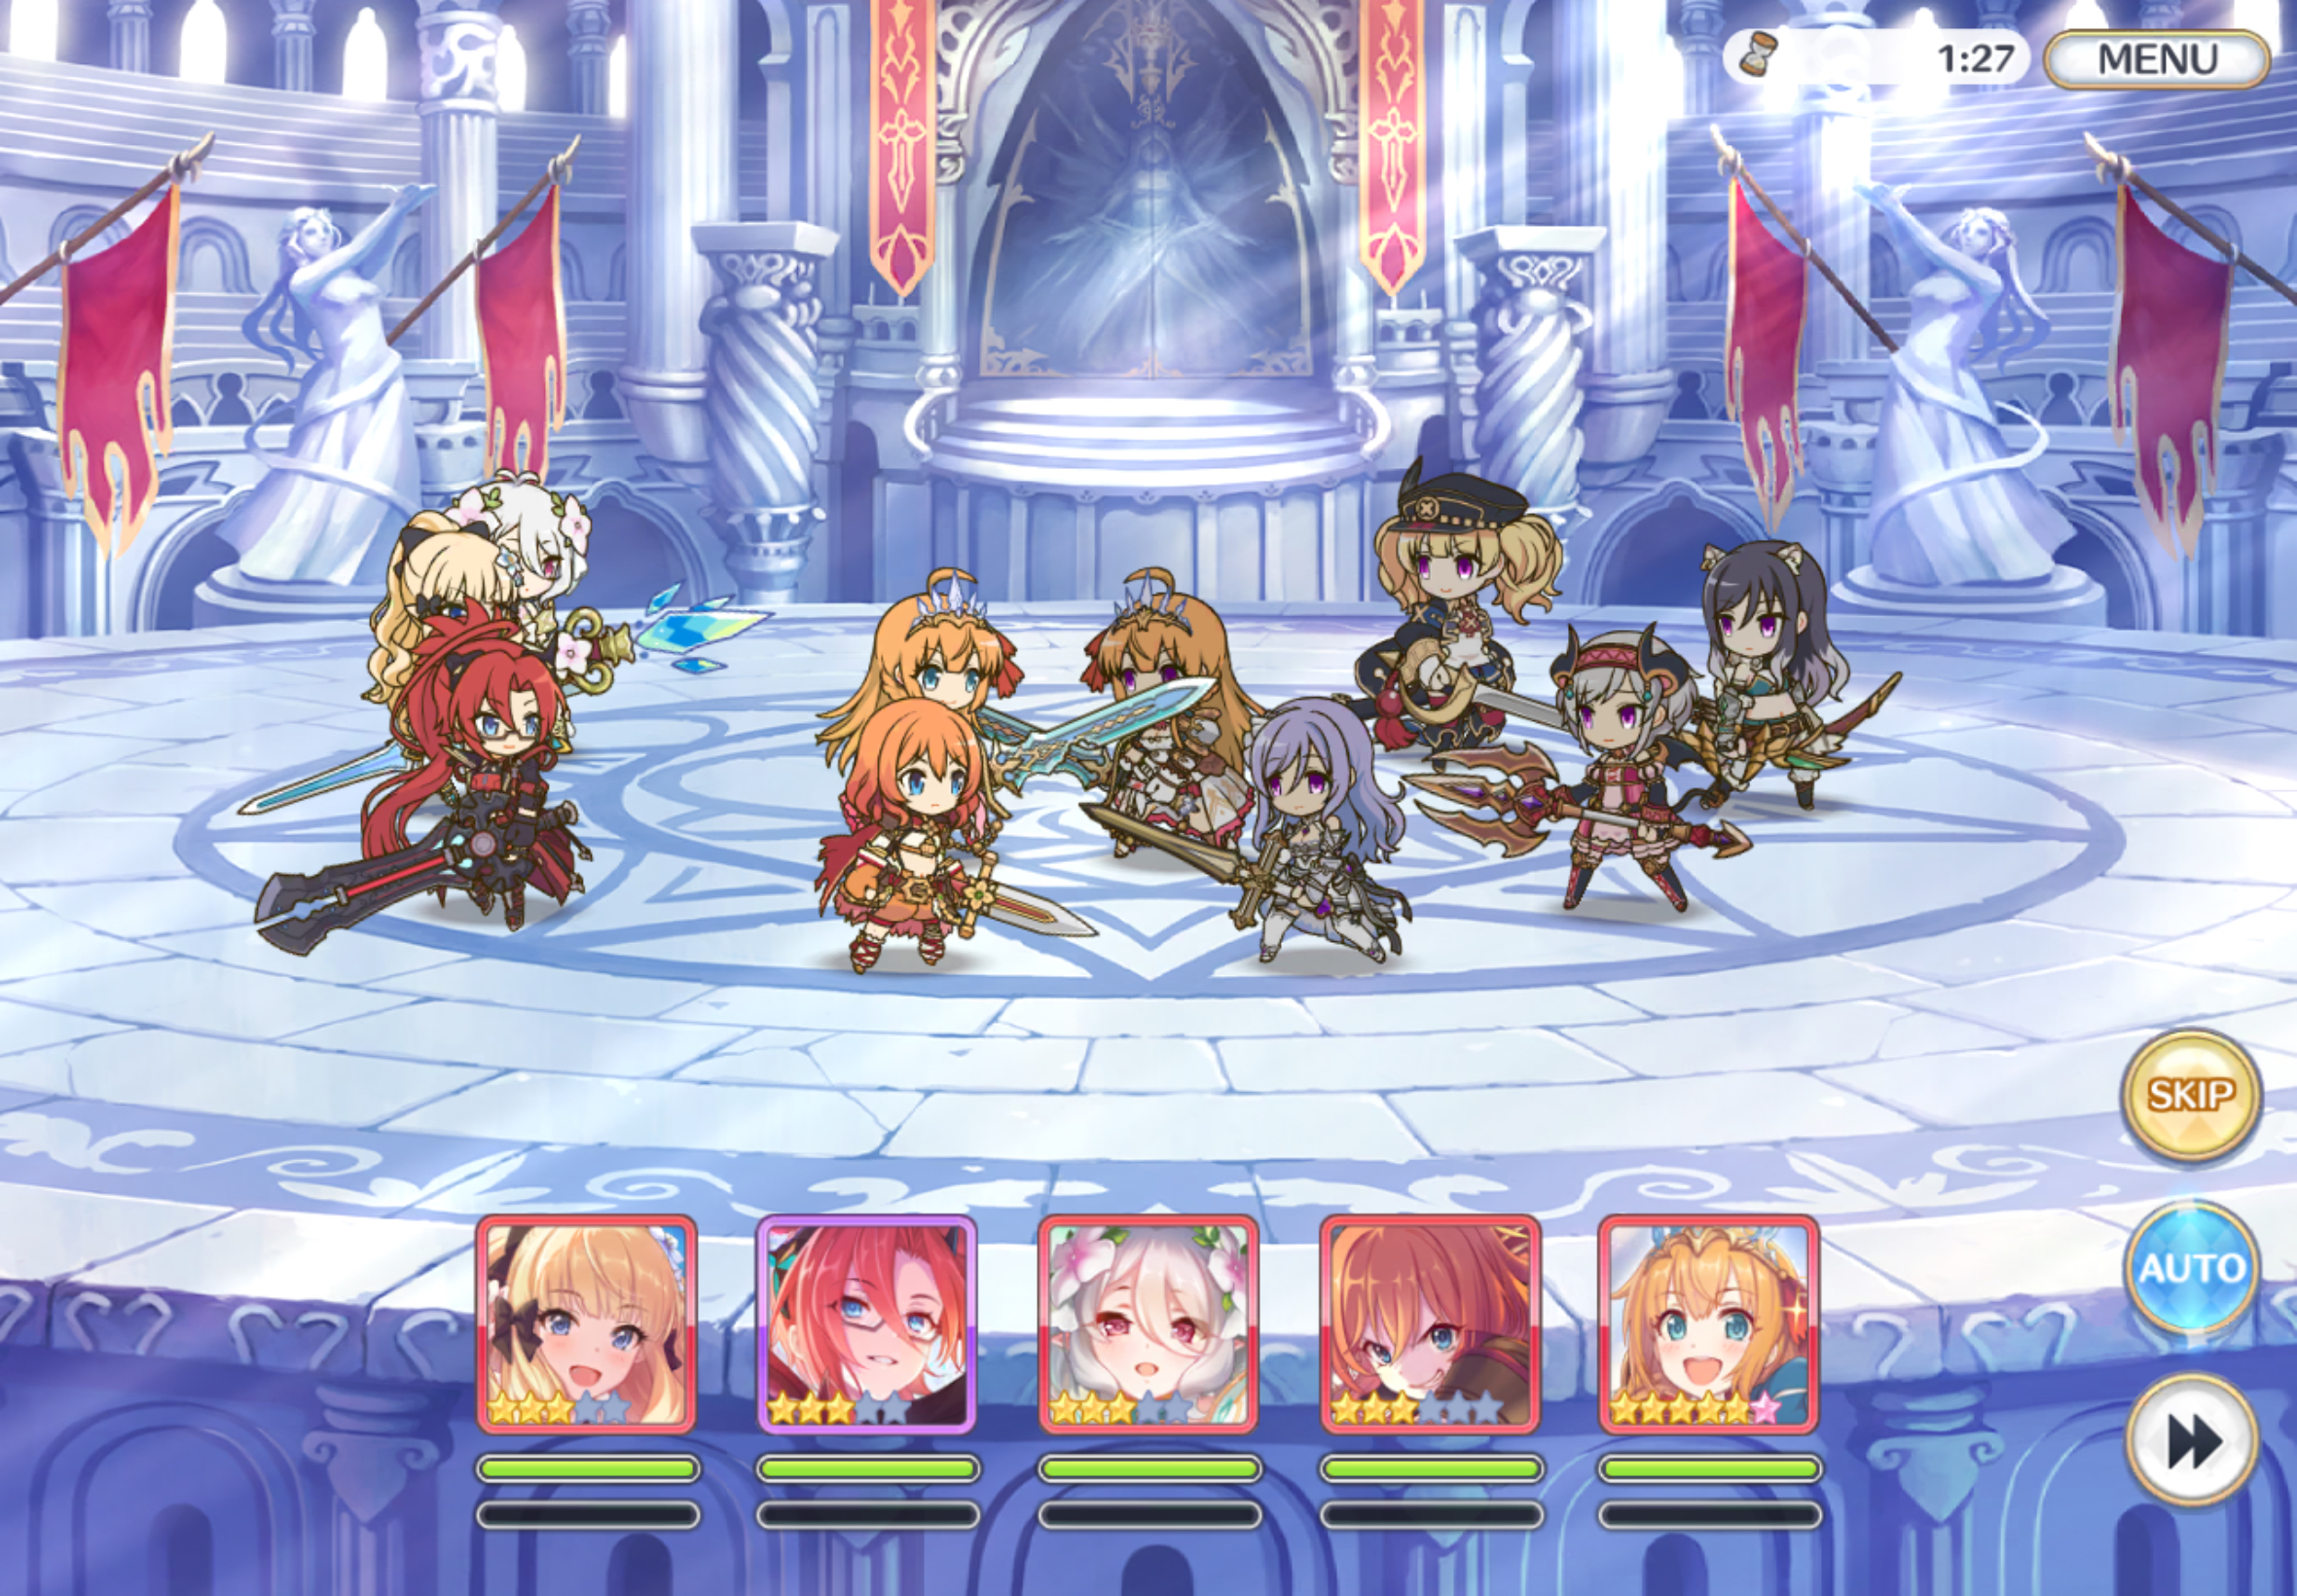
\includegraphics[width=8cm]{figure/related-work-princon-arena.png}
	\captionof{figure}[Game Example: Princess Connect! Re:Dive (Arena Section)]{Game Example: Princess Connect! Re:Dive (Arena Section)
		\\ Source: Cygames Inc. (2023). Princess Connect! Re:Dive. Screenshot by Author.}
	\label{fig:related-work-princon-arena}
	\end{minipage}

	\item Omega \\
	Omega is a puzzle game developed by ORIGIN Systems, Inc in 1989 \cite{mobygamesomega}. The game lets players program tanks by using a built-in text editor with a script that is similar to BASIC. The player can learn how to write a program by using it in the gameplay to pass the game’s missions and progress through the game. This game is similar to our project because the project was designed to teach the players about the genetics algorithm by incorporating it with the gameplay and game progression and make the player learn by applying the lesson through the puzzle we designed. \\
	\begin{minipage}[c]{\textwidth}\centering
	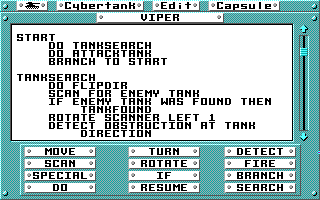
\includegraphics[width=8cm]{figure/related-work-omega-code.png}
	\captionof{figure}[Game Example : Omega (Code Writing Section)]{Game Example : Omega (Code Writing Section) \cite{mobygamesomega}}
	\label{fig:related-work-omega-code}
	\end{minipage}
	\begin{minipage}[c]{\textwidth}\centering
	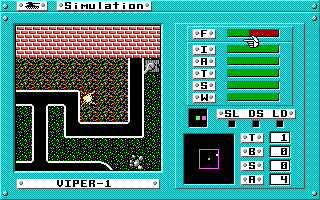
\includegraphics[width=8cm]{figure/related-work-omega-sim.png}
	\captionof{figure}[Game Example : Omega (Simulation Section)]{Game Example : Omega (Simulation Section) \cite{mobygamesomega}}
	\label{fig:related-work-omega-sim}
	\end{minipage}

	\item Super Auto Pets \\
	Super Auto Pets is a free-to-play auto-battler created by Team Wood Games, publicly released on Steam on 24 September 2021, before later released on mobile platforms. Players prepare their teams by buying new pets from a randomized pool and purchasing food to enhance their pets in the preparation phase as in Figure~\ref{fig:related-work-sap1}. Then they can send their pets to battle with other players in the battle phase as in Figure~\ref{fig:related-work-sap2}. These pets battle automatically, as both pets on the front row will attack each other simultaneously; if one's health point reduces to zero, it will faint and be out of combat. After the impact concludes, the most frontal pets strike again until a team, or both, has no pets left standing. Same as Princess Connect! Redive, we also extracted some of the battle features into our game. \\
	The game contains varieties of pets with different kinds of stats and skills for players to use in their team, letting players discover ways to synergize their pets and food the best within given limited resources, satisfying discovery fun. The game does not require players to make decisions quickly, and they can exit the game anytime during the preparation phase, thus making the game considered casual and able to satisfy players' submission fun. \\
	\begin{minipage}[c]{\textwidth}\centering
	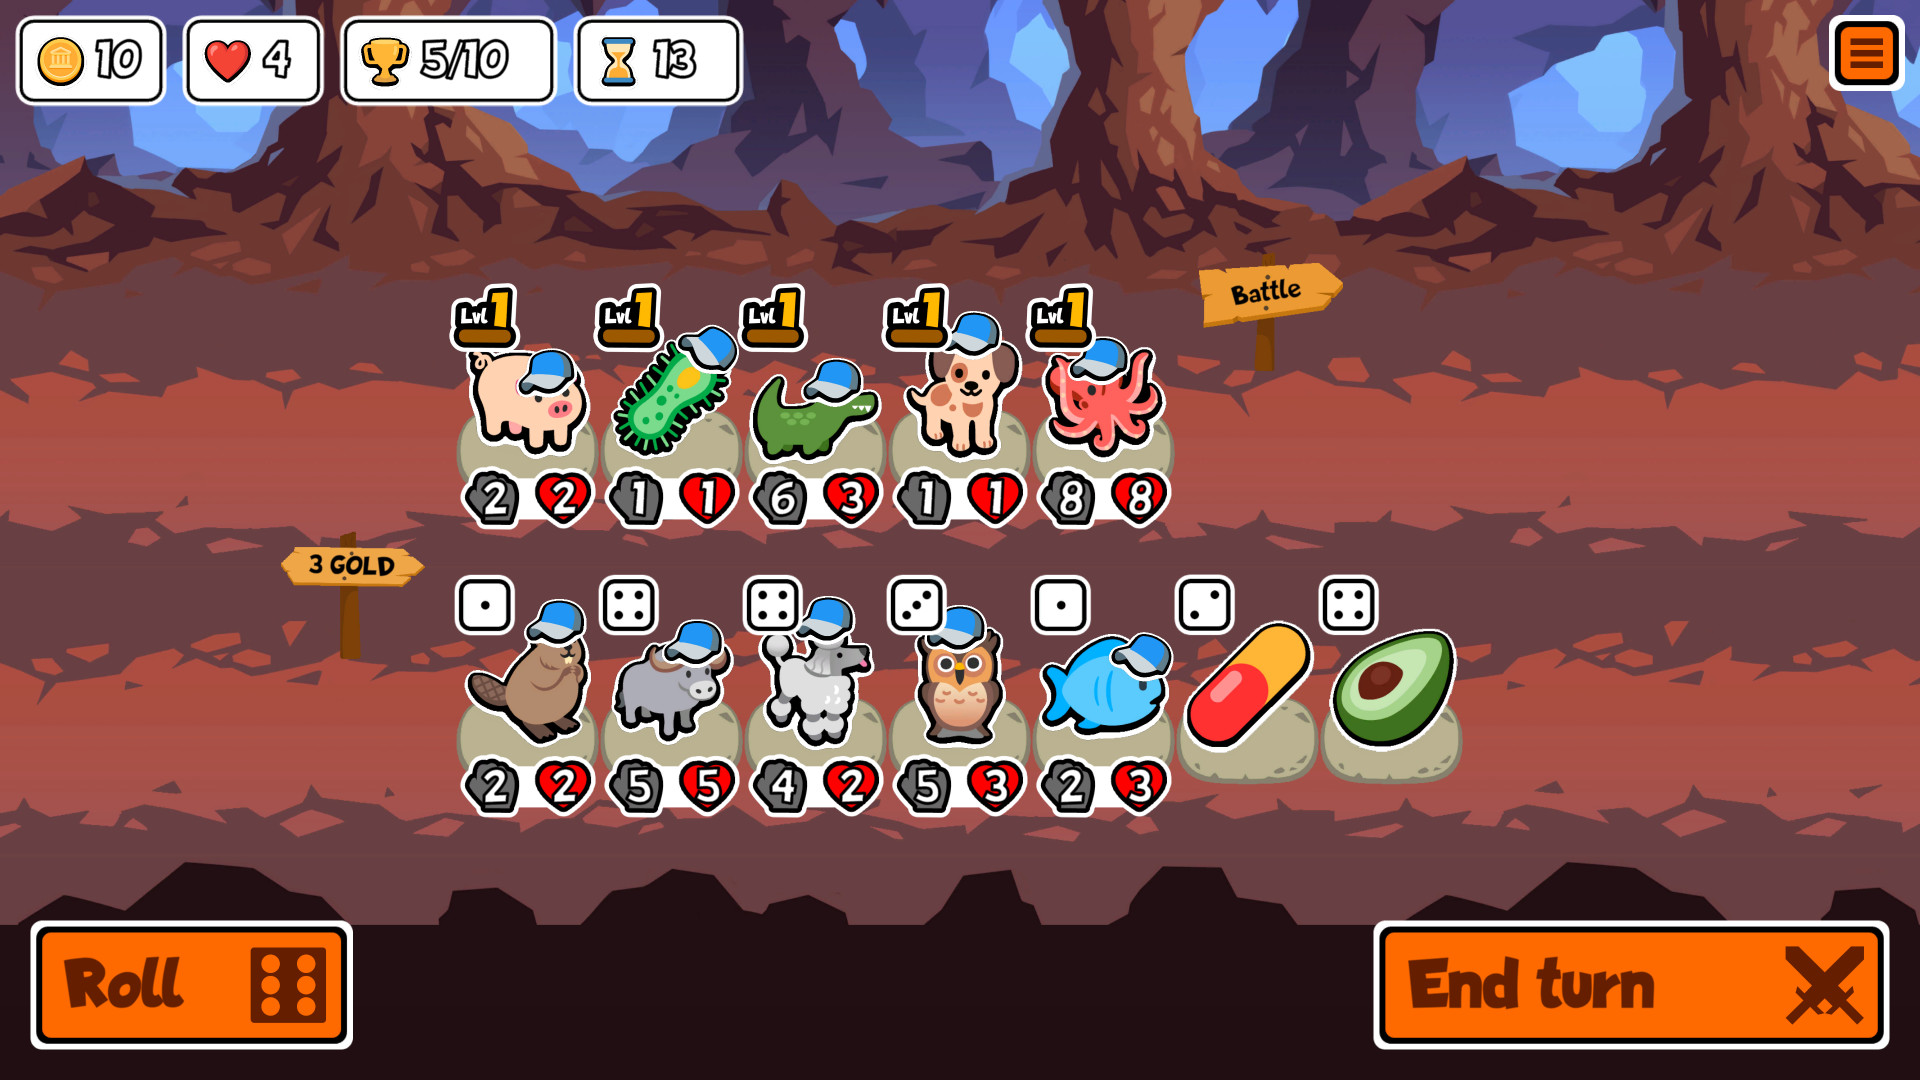
\includegraphics[width=8cm]{figure/related-work-sap1.png}
	\captionof{figure}[Game Example: Super Auto Pets (Preparation Phase)]{Game Example: Super Auto Pets (Preparation Phase) 
		\\ Source: \href{https://store.steampowered.com/app/1714040/Super_Auto_Pets/}{Super Auto Pets on Steam}}
	\label{fig:related-work-sap1}
	\end{minipage}
	\begin{minipage}[c]{\textwidth}\centering
	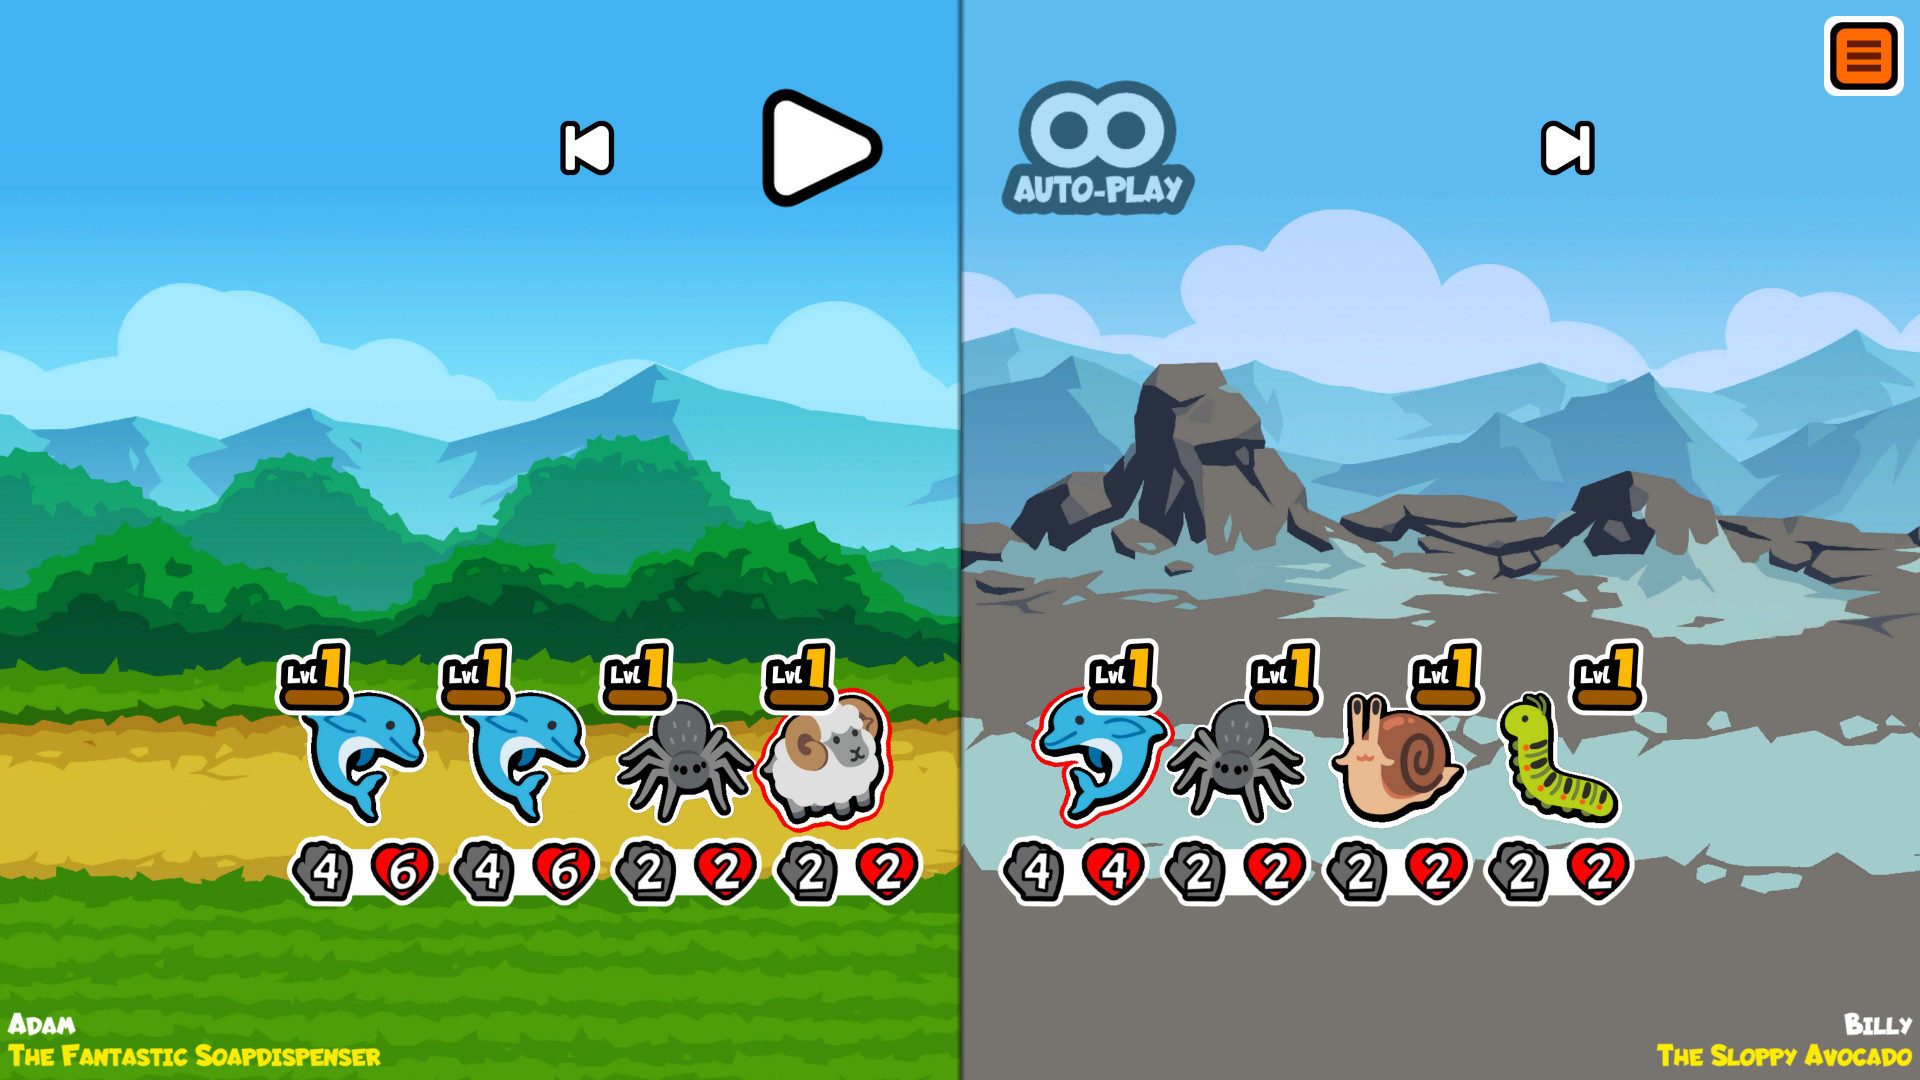
\includegraphics[width=8cm]{figure/related-work-sap2.png}
	\captionof{figure}[Game Example: Super Auto Pets (Battle Phase)]{Game Example: Super Auto Pets (Battle Phase) 
		\\ Source: \href{https://store.steampowered.com/app/1714040/Super_Auto_Pets/}{Super Auto Pets on Steam}}
	\label{fig:related-work-sap2}
	\end{minipage}
\end{enumerate}



%%%%%%%%%%%%%%%%%%%%%%%%%%%%%%%%%%%%%%%%%%%%%%%%%%%%%
%%%%%%%%%%%%%%%%%%%%%%%%%%%%%%%%%%%%%%%%%%%%%%%%%%%%%
%%%%%%%%%%%%%%%%%%%%%%%%%%%%%%%%%%%%%%%%%%%%%%%%%%%%%
\chapter{Methodology and Design}
\hspace{2em}In general, developing Digital Educational Games (DEG) has 2 main approaches. The first way is to design Computer Assisted Instruction (CAI) based on the learning topics or outcomes, then adapt it by adding the gameplay to cover the learning content to create the educational game. The second approach is reversing the first one. The game is designed first, then add a component of the learning content into the existing game to change it to be an educational game. Since we focus on the education part and already have scoped the content, we decide to develop our game using the first approach. This is one of the reasons we apply the ADDIE model in our development process.

\hspace{2em}This chapter will cover the analysis and design of both the education and gameplay aspects. The design based on the theory will be discussed. We will explain what our game contains and how it works. To clarify our idea of a design, the various diagrams and images will be also shown.

%%%%%%%%%%%%%%%%%%%%%%%%%%%%%%%%%%%%%%%%%%%%%%%%%%%%%%%%%%%%%%%%%%
%%%%%%%%%%%%%%%%%%%%%%%%%%%%%%%%%%%%%%%%%%%%%%%%%%%%%%%%%%%%%%%%%%
\section{Analysis}
Using the ADDIE model, the first task to do is the analysis of the problem and related detail.

%%%%%%%%%%%%%%%%%%%%%%%%%%%%%%%%%%%%%%%%%%%%%%%%%%%%%%%%%%%%%%%%%%
\subsection{Problem Statement}
As we mentioned in the background of the project in the first chapter, we recognize that game popularity is continuously increasing, and the attention to computer knowledge should be on the same trend. But some fields of computer knowledge like the Genetic Algorithm are hard to understand. Since the game has great potential as a learning tool and there is no educational game for learning such a topic, we decided to create an educational game to help people who are interested in such a topic can learn about Genetic Algorithms simply.

%%%%%%%%%%%%%%%%%%%%%%%%%%%%%%%%%%%%%%%%%%%%%%%%%%%%%%%%%%%%%%%%%%
\subsection{Target Audience}
People who want to learn about Genetic Algorithms, especially university students who are studying in the relevant faculties such as computer engineering. The target can be divided into 2 groups which are those who have never learned this topic before and those who have studied before but want to understand more.


%%%%%%%%%%%%%%%%%%%%%%%%%%%%%%%%%%%%%%%%%%%%%%%%%%%%%%%%%%%%%%%%%%
%%%%%%%%%%%%%%%%%%%%%%%%%%%%%%%%%%%%%%%%%%%%%%%%%%%%%%%%%%%%%%%%%%
\section{Design}
The main task of the designing phase focuses on defining the learning-related details which we will use the Outcome-based Education concept. Since our project is an educational game, there is also the design related to the game which will be described in the format of a game design document, for example, game overview, gameplay and mechanics, and so on.

%%%%%%%%%%%%%%%%%%%%%%%%%%%%%%%%%%%%%%%%%%%%%%%%%%%%%%%%%%%%%%%%%%
\subsection{Outcome-based Education (OBE) Design}
Applying the OBE concept, the education module is designed according to the triangle of effective learning which starts with the designing of the learning outcomes, followed by an assessment, and the teaching and learning method.

\begin{itemize}
	\item Learning Outcomes \\
	As we mentioned in the scope of the project, there are several educational topics involving genetic algorithms and real-world problems that can be solved using such algorithms. \\
	Using the OBE concept, we must focus on the outcome in a form of the ability that the learner should gain \cite{kmuttobe}. So, we analyze those topics, summarize them, and figure out the core concept and skill the learner should be able to do. After consideration, we set our learning outcome using the concept of OBE together with a SMART(TT) characteristics and an action verb from the level of learning in Bloom's taxonomy \cite{christine2021tophat} resulting in a single ultimate outcome which is: \\
	The learner is able to model the algorithm for solving a real-world problem using the proper problem encoding and decoding, parent selection method, crossover method, and improvement technique including elitism and mutation.\\
	The detailed criteria and method for measuring whether the learner achieves the outcome will be described in the next assessment session.

	\item Assessment \\
	After the learning outcome is designated, the next step is designing the assessment method. The typical way of the assessment is obviously a test in a form of an exam like the multiple-choice question or the writing exam. Since we decide to develop the educational game by designing the Computer Assisted Instruction (CAI) and adding the gameplay to it later, we create the criteria based on those typical assessing methods.
	For the sake of clarity and measurability, we break down the learning outcome into several criteria, grade each criterion using the Likert performance scale, and specify the condition to achieve each level in the scale using the action verb with a proper and enough detail qualifying phrase. The final assessment rubric consists of 4 criteria and at most 5 levels of performance as it is shown in Table~\ref{tbl:rubric}.

% Please add the following required packages to your document preamble:
% \usepackage{multirow}
% \usepackage{longtable}
% Note: It may be necessary to compile the document several times to get a multi-page table to line up properly
\begin{longtable}{|l|lllll|}
\caption{Rubric for Assessing the Learner}
\label{tbl:rubric}\\
\hline
\multicolumn{1}{|c|}{\multirow{2}{*}{Criteria}} &
  \multicolumn{5}{c|}{Performance descriptors} \\ \cline{2-6} 
\multicolumn{1}{|c|}{} &
  \multicolumn{1}{c|}{Level 1} &
  \multicolumn{1}{c|}{Level 2} &
  \multicolumn{1}{c|}{Level 3} &
  \multicolumn{1}{c|}{Level 4} &
  \multicolumn{1}{c|}{Level 5} \\ \hline
\endhead
%
\begin{tabular}[c]{@{}l@{}}The learner is \\ able to encode \\ the knapsack \\ problem as \\ the chromosome \\ and is able to \\ decode it.\end{tabular} &
  \multicolumn{1}{l|}{\begin{tabular}[c]{@{}l@{}}Able to explain \\ the problem,\\ constraint, \\ and goal of \\ the Standard, \\ Multidimensional, \\ and Multiple \\ Knapsack \\ Problem.\end{tabular}} &
  \multicolumn{1}{l|}{\begin{tabular}[c]{@{}l@{}}Able to \\ demonstrate \\ the chromosome \\ encoding and \\ decoding of \\ the Standard and \\ Multidimensional \\ Knapsack \\ Problem.\end{tabular}} &
  \multicolumn{1}{l|}{\begin{tabular}[c]{@{}l@{}}Able to \\ demonstrate \\ the \\ chromosome \\ encoding and \\ decoding of \\ a Multiple \\ Knapsack \\ Problem.\end{tabular}} &
  \multicolumn{1}{l|}{\begin{tabular}[c]{@{}l@{}}Able to \\ solve the \\ chromosome \\ encoding and \\ decoding of \\ the Standard and \\ Multidimensional \\ Knapsack \\ Problem.\end{tabular}} &
  \begin{tabular}[c]{@{}l@{}}Able to \\ solve the \\ chromosome \\ encoding and \\ decoding of \\ a Multiple \\ Knapsack \\ Problem.\end{tabular} \\ \hline
\begin{tabular}[c]{@{}l@{}}The learner is \\ able to solve \\ the parent \\ chromosome \\ selection \\ problem in \\ the Genetic \\ Algorithm.\end{tabular} &
  \multicolumn{1}{l|}{\begin{tabular}[c]{@{}l@{}}Able to explain \\ the meaning \\ and purpose \\ of a parent \\ chromosome \\ selection in \\ a Genetic \\ Algorithm.\end{tabular}} &
  \multicolumn{1}{l|}{\begin{tabular}[c]{@{}l@{}}Able to \\ demonstrate \\ the process \\ of the \\ Tournament\\ -based \\ Selection.\end{tabular}} &
  \multicolumn{1}{l|}{\begin{tabular}[c]{@{}l@{}}Able to \\ demonstrate\\ the process \\ of the Roulette\\ Wheel \\ Selection and \\ Rank-based \\ Selection.\end{tabular}} &
  \multicolumn{1}{l|}{\begin{tabular}[c]{@{}l@{}}Able to \\ solve parent \\ selection \\ problems \\ using \\ Tournament\\ -based \\ Selection.\end{tabular}} &
  \begin{tabular}[c]{@{}l@{}}Able to \\ solve parent \\ selection \\ problems \\ using \\ Roulette \\ Wheel \\ Selection \\ and \\ Rank-based \\ Selection.\end{tabular} \\ \hline
\begin{tabular}[c]{@{}l@{}}The learner is \\ able to solve \\ the chromosome \\ crossover \\ problem in \\ the Genetic \\ Algorithm.\end{tabular} &
  \multicolumn{1}{l|}{\begin{tabular}[c]{@{}l@{}}Able to explain \\ the meaning \\ and purpose of \\ a chromosome \\ crossover \\ in a Genetic \\ Algorithm.\end{tabular}} &
  \multicolumn{1}{l|}{\begin{tabular}[c]{@{}l@{}}Able to classify \\ between \\ Single-point \\ Crossover, \\ Two-point \\ Crossover, \\ and Uniform \\ Crossover.\end{tabular}} &
  \multicolumn{1}{l|}{\begin{tabular}[c]{@{}l@{}}Able to \\ demonstrate \\ the process \\ of the \\ Single-point \\ Crossover and \\ Two-point \\ Crossover.\end{tabular}} &
  \multicolumn{1}{l|}{\begin{tabular}[c]{@{}l@{}}Able to \\ solve the \\ chromosome \\ crossover \\ problem \\ using the \\ Single-point \\ Crossover \\ and \\ Two-point \\ Crossover.\end{tabular}} &
   \\ \hline
\begin{tabular}[c]{@{}l@{}}The learner is \\ able to identify \\ the basic method \\ of improvement \\ technique in \\ the Genetic \\ Algorithm \\ including \\ elitism and \\ mutation.\end{tabular} &
  \multicolumn{1}{l|}{\begin{tabular}[c]{@{}l@{}}Able to explain \\ the meaning \\ and purpose \\ of Elitism \\ and mutation \\ in Genetic \\ Algorithm.\end{tabular}} &
  \multicolumn{1}{l|}{\begin{tabular}[c]{@{}l@{}}Able to classify \\ between Elitism, \\ Bit Flip Mutation, \\ Flip Bit Mutation, \\ and \\ Boundary \\ Mutation.\end{tabular}} &
  \multicolumn{1}{l|}{\begin{tabular}[c]{@{}l@{}}Able to identify \\ the type of \\ improvement \\ technique \\ including \\ Elitism, \\ Bit Flip \\ Mutation, \\ Flip Bit \\ Mutation, \\ and \\ Boundary \\ Mutation.\end{tabular}} &
  \multicolumn{1}{l|}{} &
   \\ \hline
\end{longtable}
	The assessment rubric alone cannot evaluate the learner's performance. It needs some evidence, the result of the learner's action, to pair up with the criteria for determining the actual level of the learner. We divide the type of evidence into 3 groups based on the level of learning. The assessment activity for each group is designed based on the appropriate alignment in \cite{eberly2022why}. For example, the type of the applying outcome should be evaluated using the activity causing the learner to determine what method to use and use such procedures to solve the problem. All the types of evidence we will use are listed below.
	\begin{enumerate}
		\item  The evidence involving explaining, classifying, and identifying is a choice that the learner chooses for the given question or situation.
		\item  The evidence involving demonstrating is a result of a puzzle that they must complete with the correct processes, generating the result corresponding to the expected result.
		\item  The evidence involving problem-solving is a result of a puzzle similar to the demonstration, but the puzzle in this level gives more choice to the player. So, the player must decide what type of method to perform from the given description through the puzzle's element selection. Then the player should perform the method like in the demonstration.
	\end{enumerate}
	The evidence involving explaining and demonstrating for assessment levels 1 to 3 will be collected from the test after completing the lesson in the research lab section of the game and All the types of evidence of every level will be collected more from the result of the puzzles used for fixing the facilities when they are broken.

	\item Learning and Teaching \\
	When the learning outcome and assessment method are all designed, the final task of the education planning is to design the learning and teaching including the materials and activities. The material will be developed using multimedia mostly in the style of the image and description text. 

	\begin{minipage}[c]{\textwidth}\centering
	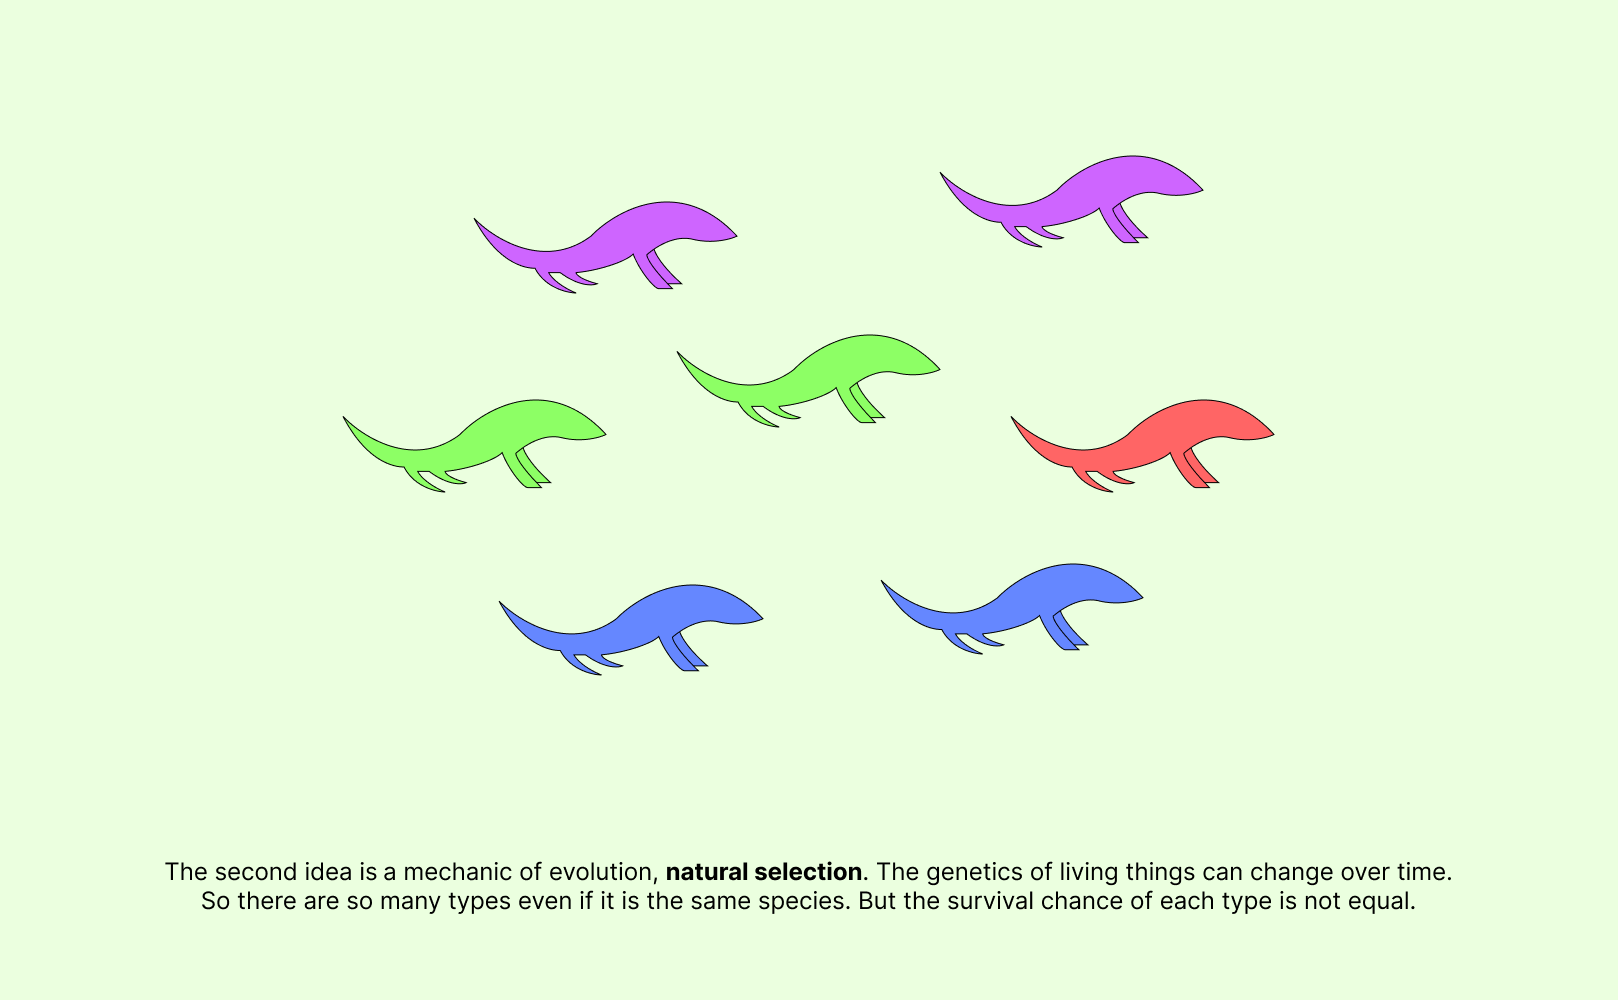
\includegraphics[width=12cm]{figure/design-learnmat-natselect1.png}
	\captionof{figure}{Example Material for Learning Natural Selection}
	\label{fig:design-learnmat-natselect1}
	\end{minipage}

	Figure~\ref{fig:design-learnmat-natselect1} is an example of the material we have already prepared for Natural Selection, one of the basic biology concepts the Genetic Algorithm is based on. The material in the figure includes the image on the center and description about natural selection at the bottom. The full learning materials are in Appendix. %~\ref{appendix:learning-material}.

%	\begin{minipage}[c]{\textwidth}\centering
%	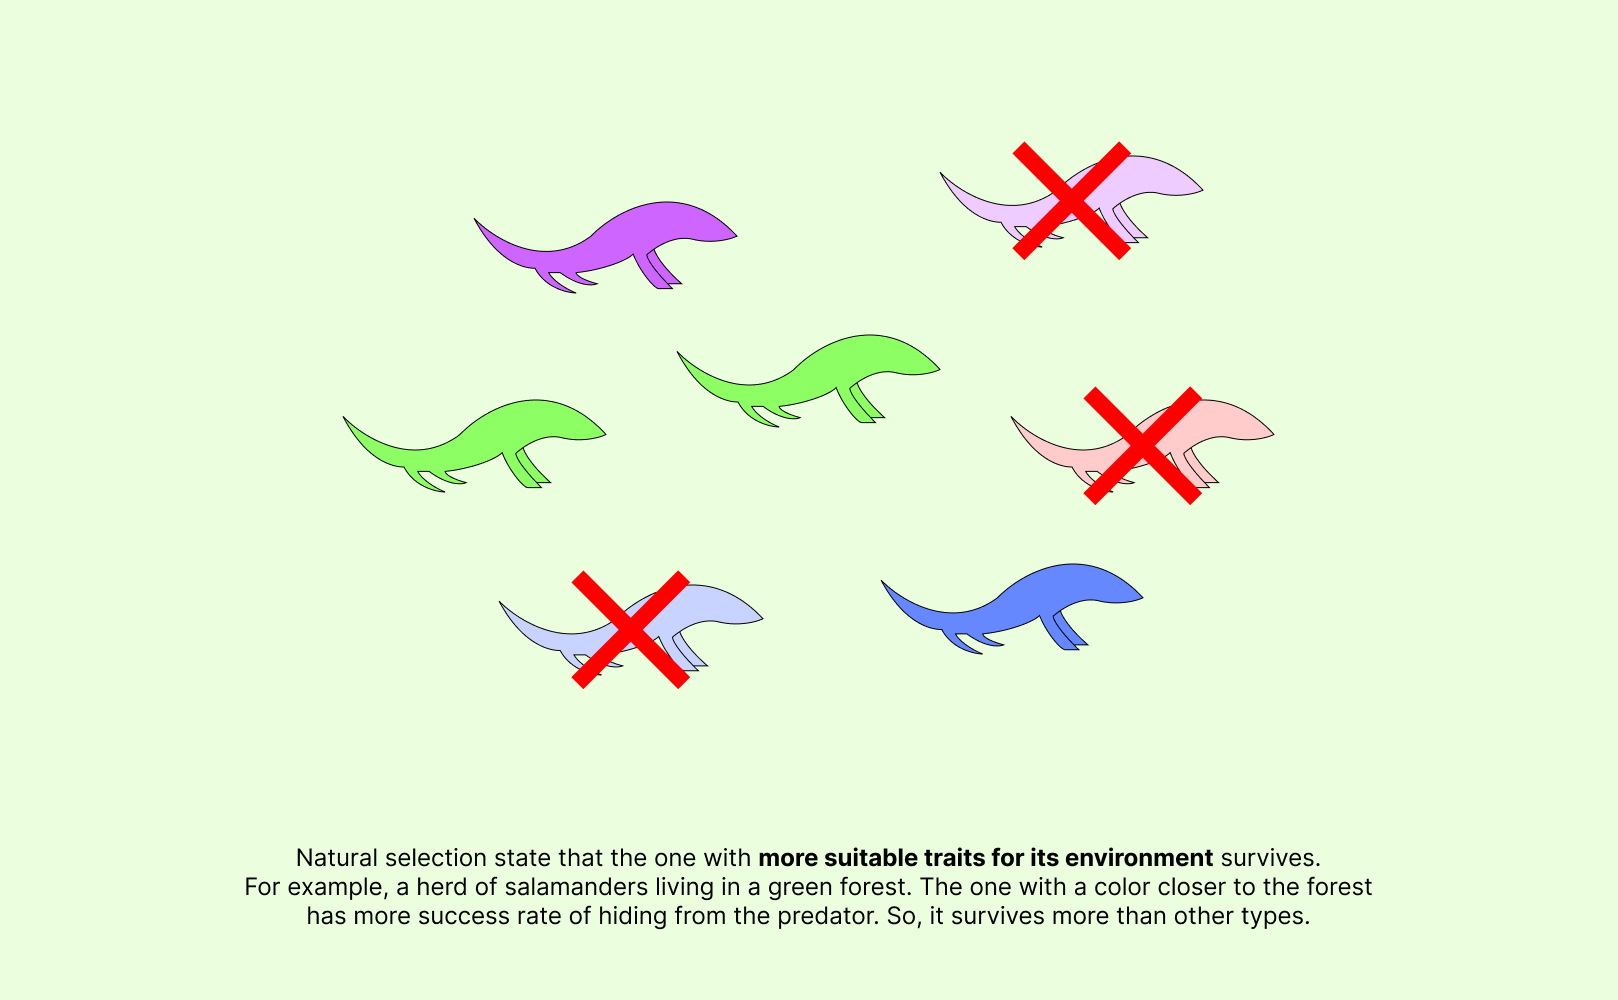
\includegraphics[width=12cm]{figure/design-learnmat-natselect2.png}
%	\captionof{figure}{Example Material for Learning Natural Selection (2/3)}
%	\label{fig:design-learnmat-natselect2}
%	\end{minipage}
%
%	\begin{minipage}[c]{\textwidth}\centering
%	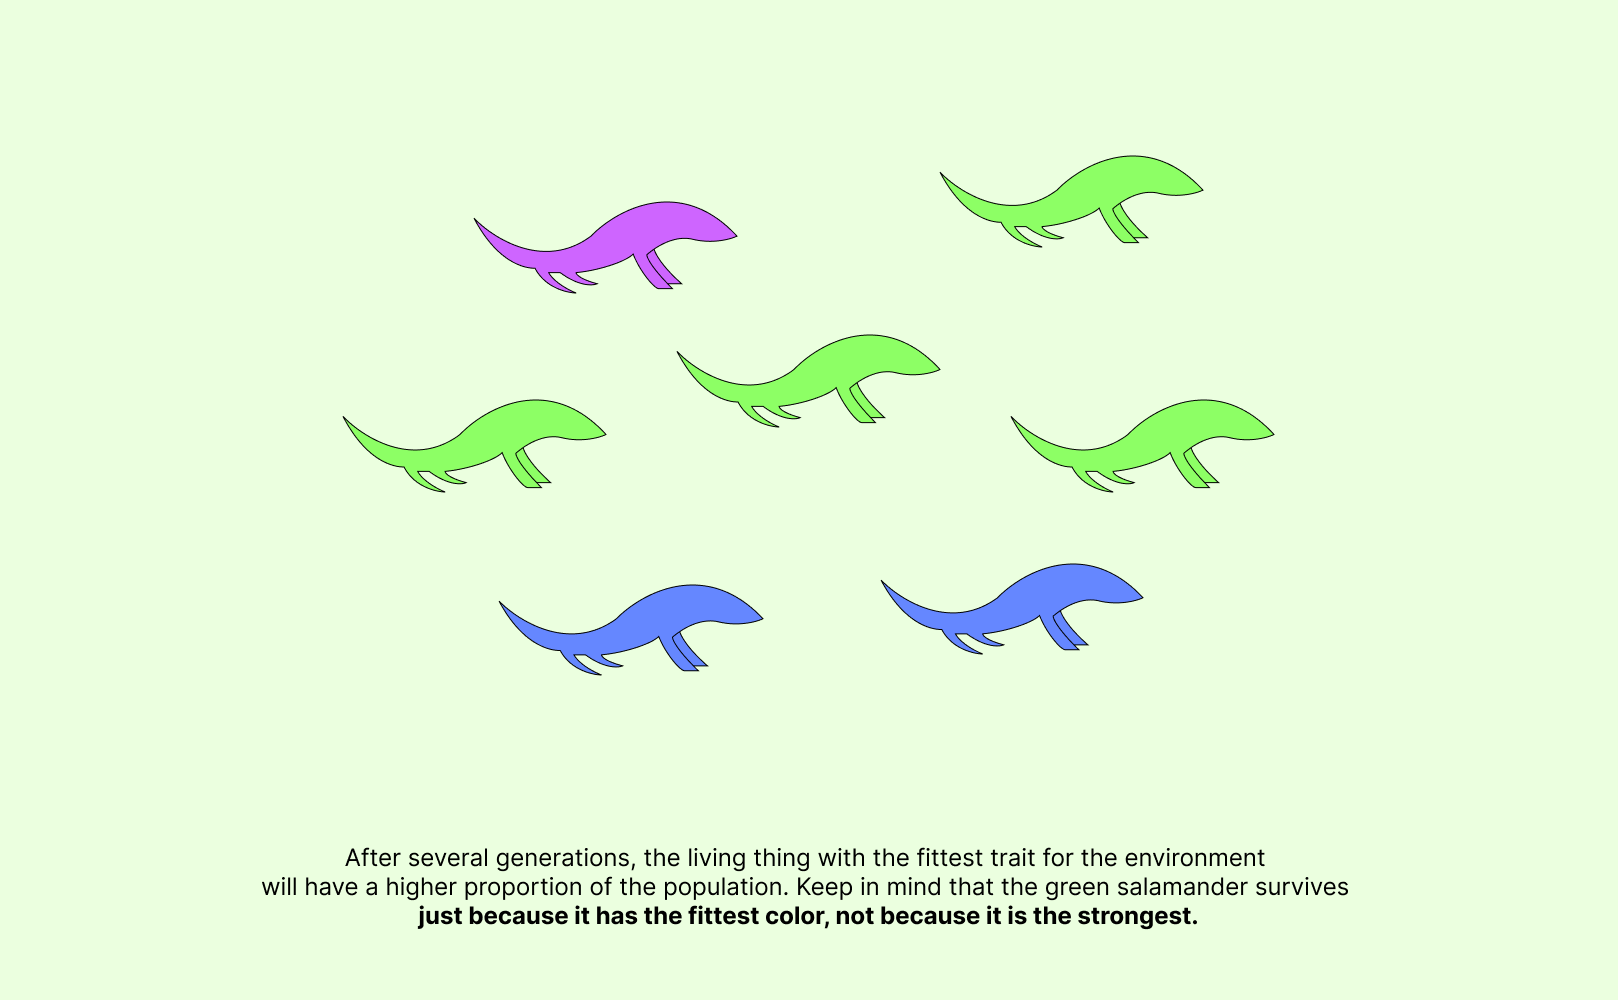
\includegraphics[width=12cm]{figure/design-learnmat-natselect3.png}
%	\captionof{figure}{Example Material for Learning Natural Selection (3/3)}
%	\label{fig:design-learnmat-natselect3}
%	\end{minipage}

	When adding the component of the game, the material will be adjusted and integrated with the game story. There also will be a Research Lab system involving the material which will be described in detail in the Game Overview section. \\
	The next issue to concern is the teaching and learning activities. Since we aim to create an educational game, we use the great advantage of using the game, the high level of interactive activities, as the learning activity in the manner of experiential learning. To be clear, the learning activity is the puzzle gameplay similar to the gameplay used for the assessment. But in the aspect of learning and teaching, there will be a guide that tells the player what and how the puzzle works. For example, the puzzle for assessing the demonstration of the player will be evaluated based on the type of process and the sequence the player chooses. But when it is used as a learning activity, the game will guide the player on what process to choose at each time step.

\end{itemize}

%%%%%%%%%%%%%%%%%%%%%%%%%%%%%%%%%%%%%%%%%%%%%%%%%%%%%%%%%%%%%%%%%%
\subsection{Game Design Theory Application}
%Game Design Theories used for designing the game of the project are as follows: 
%
%\begin{itemize}
%\item Natural Funativity \\
%The game we designed mainly consists of three of the categories from Natural Funativity by Noah Falstein. The categories we used will be listed as follows:
%\begin{enumerate}
%	\item Physical Fun \\
%	We design the game to make players solve the puzzles by making the players move and click their mouse and use hand-eye coordination to solve the puzzles.
%	\item Social Fun \\
%	We design the game to have a story and interaction between the 
%players and nonplayer characters (NPC).
%	\item Mental Fun \\
%	We design the game to make players solve the puzzles from the lesson and manage farms and factories with money and resources in order to progress through the game.
%\end{enumerate}
\hspace{2em}The game we designed mainly focuses on Mental Fun categories of Natural Funativity by Noah Falstein. We design the game to make players solve the puzzles from the lesson and manage farms and factories with money and resources in order to progress through the game.


%\item Maslow’s Hierarchy of Needs \\
%The Hierarchy of Needs we used for the game design will be listed as follows:
%\begin{enumerate}
%	\item Physiological Needs \\
%	The players need to use money and resource to breed stronger monsters in order for them to survive the battle inside the battle arena.
%	\item Safety Needs \\
%	The players can improve the battle status of their monsters by breeding them to create a new generation of monsters and the players can improve the status of the weapon from the factories by creating a new generation of weapons.
%	\item Love and Belonging Needs \\
%	The player can interact and talk to the nonplayer character in the game story that we have designed. The player can have a connection and feel more engaged in the story.
%	\item Esteem Needs \\
%	The game will assign rank and reward for the success of the quest completion by the quality or closeness of the requested item and sent the item. The players can feel accomplished when getting high ranking and feel accomplished when finishing the game after meeting the requirements of all weapons from the factories.
%	\item Cognitive Needs \\
%	The game was designed to teach players about genetic algorithms and how to solve the problem with this knowledge.
%	\item Aesthetic Needs \\
%	The game will have a beautiful aesthetic with music to make it more pleasing to play for the players. The higher the ranking for completing the quest the more beautiful the rank is and the more powerful the weapon is the more elaborate and better it looks.
%	\item Self-Actualization Needs \\
%	The game was designed to be open to the players' play style by not limiting how the players manage the farm, factories, money, and resources. The players can choose how to spend their resources and how to obtain them by themselves.
%	\item Transcendence Needs \\
%	When the players developed their own technique on how to play the game, the player can share their knowledge with their peers by talking, video capturing, etc.
%\end{enumerate}
\hspace{2em}The game we designed caters to the needs of the players following Maslow's Hierarchy of Needs to make players feel fulfilled and have answers to their needs when playing the game. The first need is Physiological Needs where the players must obtain resources to breed stronger monsters to survive the battle inside the arena. Next is the Safety Needs where the players can improve the status of their monsters and weapons by creating new generations. For the Esteem Needs of the players we design the game to assign rank and rewards for completing quests based on the quality of the requested item to help fulfill the players when they get high rank and reward when completing the quest or win the battle in the battle arena. For the Cognitive Needs, The game was designed to teach players about genetic algorithms and how to solve the problem with this knowledge. The game's Aesthetic Needs are met through its music and visually appealing rewards with higher rankings and more powerful weapons resulting in more elaborate and appealing rewards. Lastly, the game design caters to the Self-Actualization Needs of the players by allowing them to manage their farm, factories, money, and resources according to their preferred playstyle and choose how to spend their resources and how to obtain them by themselves. The game design's hierarchy of needs is well-thought-out, providing players with an immersive and satisfying experience.

%\item Eight Kinds of “Fun” \\
%The kind of fun that the game we design provided will be listed as follows:
%\begin{enumerate}
%	\item Sensation - Game as sense-pleasure \\
%	The game will have a sci-fi theme aesthetic to its visual, characters, music, and sound effect from the players' interactions.
%	\item Fantasy - Game as make-believe \\
%	The game will have its own story, world, and characters to help the players feel immersed in the game we designed. The player will have a role to take and objectives to accomplish in the story.
%	\item Narrative - Game as drama \\
%	The players will take the role of the owner of a weapon company in the future. The world will be invaded by aliens and the government orders every weapon company to create a set of ultimate weapons.
%	\item Challenge - Game as obstacle course \\
%	In order for the players to manage and upgrade their farms and factories, they need to complete the quest which will be harder when the game progresses or battle in the arena which will have more difficult opponents over time.
%	\item Fellowship - Game as social framework \\
%	The game is a single-player game but the players can interact and talk to nonplayer characters in the story and from the lesson.
%	\item Discovery - Game as uncharted territory \\
%	The players can unlock more weapon factories to make different kinds of weapons with different effects when used in the battle arena.
%	\item Expression - Game as self-discovery \\
%	The players are free to spend their money and resources and can choose how to obtain more money by completing quests or battles in the battle arena.
%	\item Submission - Game as pastime \\
%	The player can choose to not send their monster to the arena and play the game by completing the quest and managing the farm and factories.
%\end{enumerate}
%
%\end{itemize}
\hspace{2em}The game we design aims to provide different kinds of fun that cater to the players' preferences. The first kind of fun is Sensation, where the game's sci-fi and fantasy theme aesthetic stimulates the senses through visuals, character design, music, and sound effects from the players' interactions. The second kind of fun is Fantasy, where the game's story, world, and characters help the players feel immersed in the game and give them a role to play with objectives to accomplish in the story. The third kind of fun is Challenge, where players must complete quests and battle opponents in the arena to obtain the resources to upgrade their farms and factories. As the game progresses, the quests and opponents become more difficult, providing a sense of accomplishment upon completion. Lastly, the game design provides Expression, where the players can freely manage their money and resources, and choose the combination of weapons and monsters for the battle arena that suits their playstyle. The game design's various kinds of fun make the game engaging and enjoyable for all types of players.

\hspace{2em}The details of the education and other activity in the game will be described in the next section. And the alignment between the learning outcome and the game activity used to assess such outcome will be explained further in Table~\ref{tbl:activity-to-achieve-puzzle} in the next chapter.

%%%%%%%%%%%%%%%%%%%%%%%%%%%%%%%%%%%%%%%%%%%%%%%%%%%%%%%%%%%%%%%%%%
\subsection{Game Overview}
	As we mentioned, we decided to develop the game using an approach in which Computer Assisted Instruction (CAI) is designed first, then adding the game systems to transform it into Digital Educational Games (DEG). The main reason for adding the game systems is to increase the external learning motivation of the player so that the player has more will for playing and learning in the game. The game overview will describe how we will create the CAI and what kind of game systems we will add.


\begin{itemize}

\item Game Concept \\
Our game will focus on three main aspects: obtaining skills, applying skills, and other activities. The player will be played as one participates in the global-guardian project, the project for creating a powerful combat force used for future fighting with the alien. To do that, the player has to research through visual novel gameplay and validate their skills using the puzzles. Then, applying their genetic algorithm skills to weapon and monster breeding. Lastly, the player can perform other activities that don't directly involve the genetic algorithm but may be related. Battles using their bred weapon and monster is an examples. \\
For the first aspect, obtaining skills, there is a set of main systems involved. The player has to research via the cutscene explaining the subject. The research result (explanation for that subject) is kept in the research lab for review in the future. After that, the player is required to pass a skill check using the puzzles. And the skill-checking results are all kept in the hall of intelligence, a place a game progress is shown and can be translated into the learning outcome evaluation further. \\
For the second aspect, applying skills, there is a set of primary supporting systems involved. The usual visual novel and puzzle gameplay that focuses on education may be boredom since the learning motivation may not be enough. To drive the motivation of the player, we design supporting systems that the player should use their learned skills to create a weapon using the weapon factory and breed the monster using monster farm. To build more facilities and unlock more weapons, the player is required to complete certain research. Since the factory and farm break down after some time passes, the player must solve the same puzzle as skill validating to fix these facilities. \\
For the last aspect, other activities, there is a set of secondary supporting systems involved. The battle arena is a system where the player can battle with the Non-Player Character (NPC) using their bred weapon and monster. There is also a side quest where the player is required to deliver a monster with some specific appearance. Another system is a random event where a random specie of Capybara walk by facilities, and the player can capture it by rapidly clicking on it. All these systems are completely optional and don't really affect education. But they can give the player great motivation to keep playing the game.


%	Our game will focus on three main aspects: monster farm, weapon factory, and research lab. The player will own a farm to breed monsters used in the arena; rewarded with money and resources to upgrade and maintain the farm. \\
%	The monster farm is based on the Genetic Algorithm, which will be covered in detail in the next topic. The farming system will let players take control of the farm and breed monsters with the Genetic Algorithm to increase their battle status used in the arena. \\
%	The weapon factory is based on how to solve real-world problems with the Genetic Algorithm. The factory can help increase monsters’ battle status but it can be broken down over time so the player needs to use their knowledge about how to solve real-world problems with the Genetic Algorithm to fix the factory. \\
% 	There is also an educational section called research lab that will teach players about the basics of the Genetic Algorithm, how the algorithm works, and how to solve real-world problems with it. Player needs to use certain resources to unlock new topics which also unlock new factories when the topic is about real-world problems.


\item Game Flow Summary \\
	As an educational game, we conduct the game flow linearly to help the player get the basic before going into more advanced subjects. Figure ~\ref{fig:design-gameflow} shows the game flow diagram in terms of progression and game systems. The player must achieve the condition at the arrow tail before being able to achieve the head of an arrow. For example, the player must obtain skill 1 to finish main quest 1.

%	The game begins with the prologue story which some of the learning content is integrated. The player will be introduced to each system in the game, especially the core system, the research lab, which is used for learning and unlocking new facilities. \\
%	After the tutorial ends, the player is free to do any activities. But in the early game, most farms and factories will be locked. The player needs to complete certain research to get a certificate or the right to build a facility. Figure~\ref{fig:design-main-game-page} show the main game page which some facility is unlocked. After players unlock and build the facility, they can use that facility in the way their want.

\begin{minipage}[c]{\textwidth}\centering
\fbox{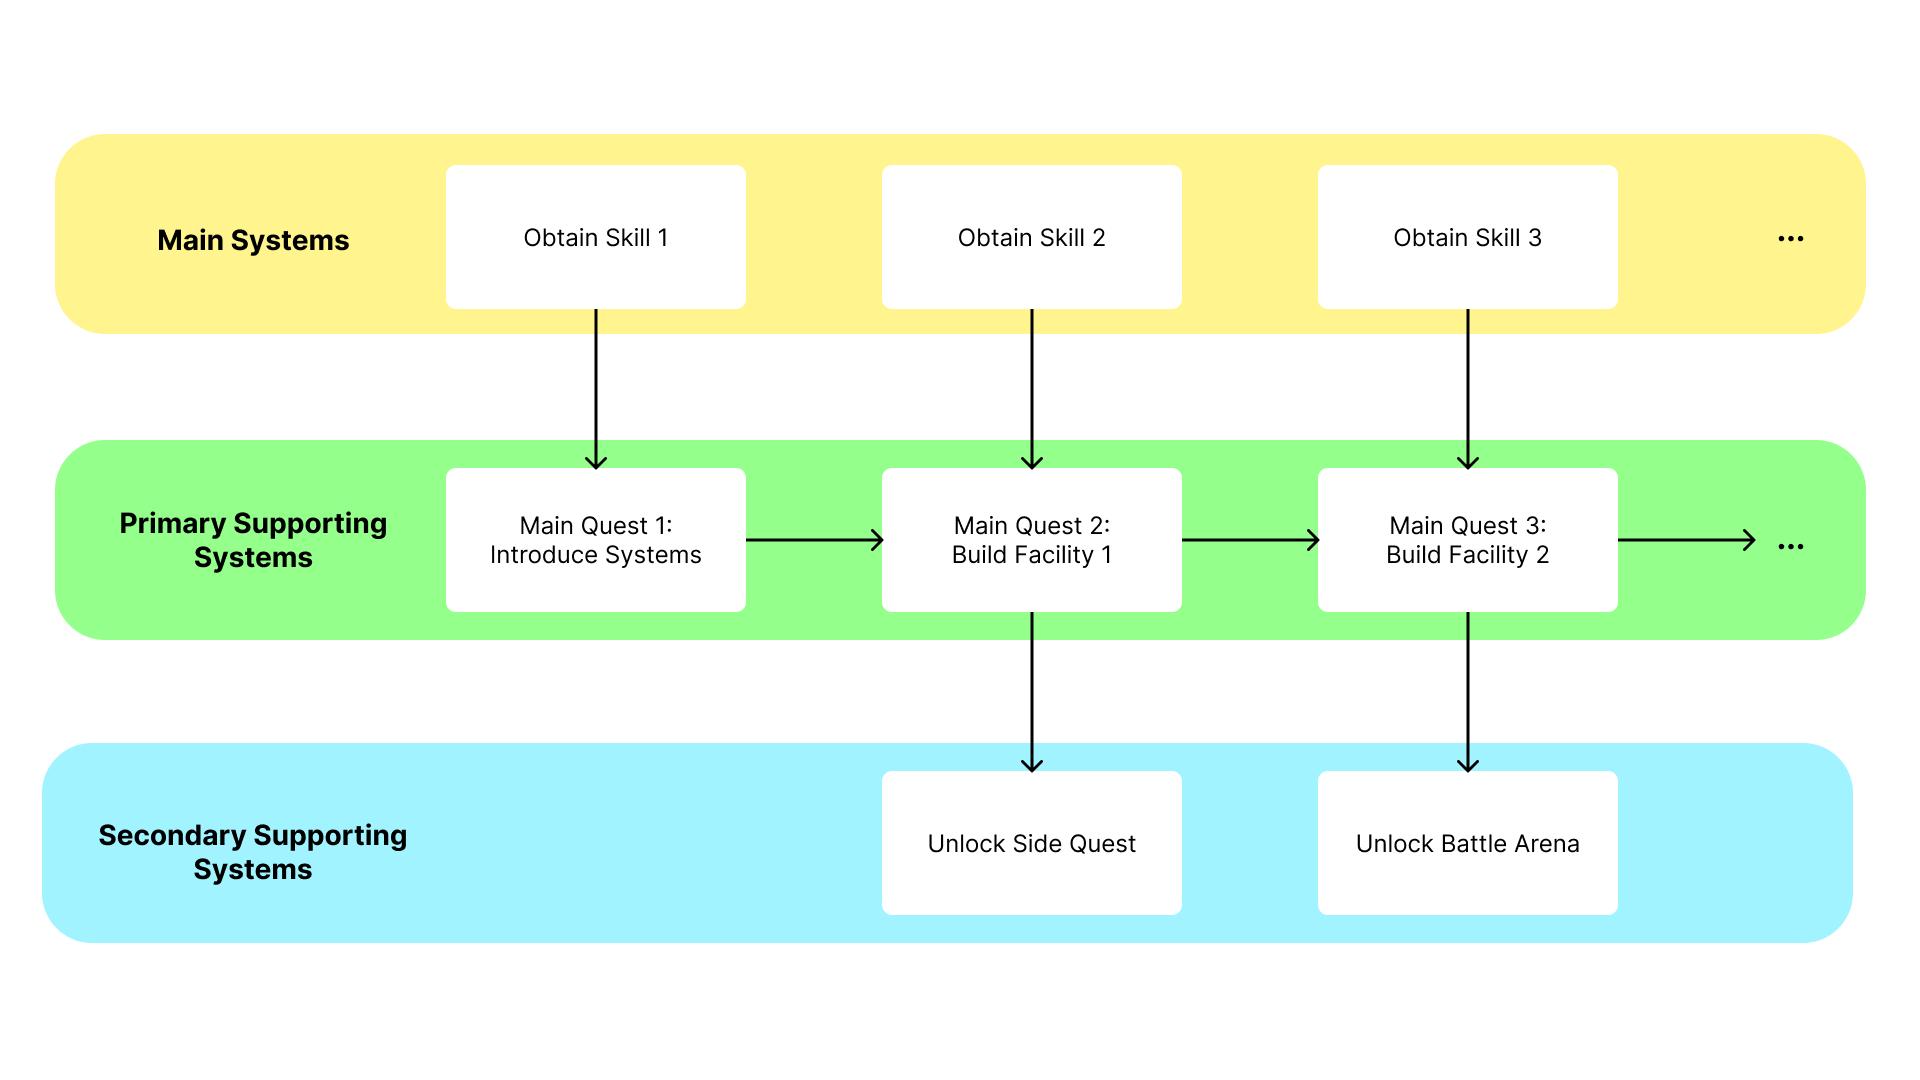
\includegraphics[width=12cm]{figure/design-gameflow.png}}
\captionof{figure}{Game Flow Diagram}
\label{fig:design-gameflow}
\end{minipage}

The game begins with the introduction to the main systems, the Research Lab and the Hall of Intelligence. After completing the early learning and getting the early skill, such as the ability to explain basic biology, the main quest will conduct the player to build more facilities that require a higher level of skill corresponding to the diagram shown in Figure~\ref{fig:design-gameflow}. Figure~\ref{fig:design-main-game-page} shows the main game page interface where the player can access any facility and all other systems.

\begin{minipage}[c]{\textwidth}\centering
\fbox{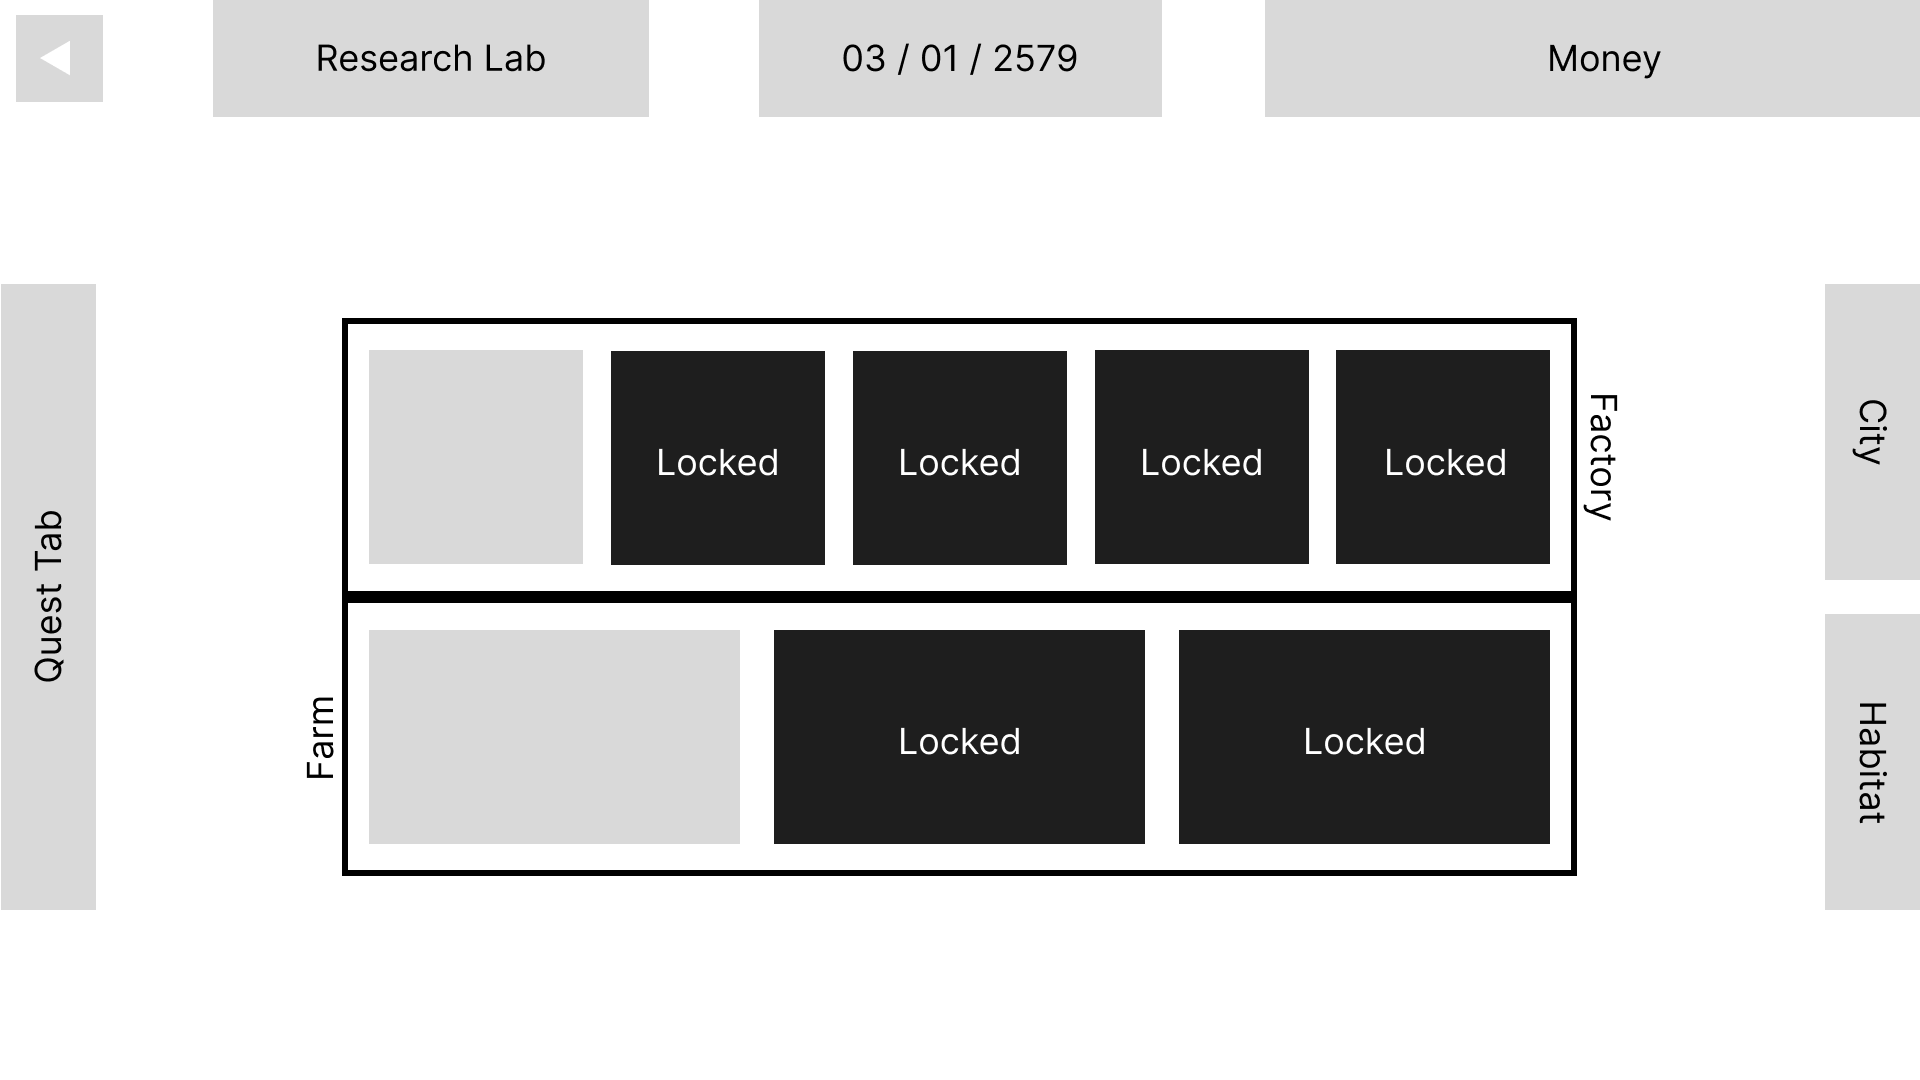
\includegraphics[width=12cm]{figure/design-main-game-page.png}}
\captionof{figure}{Main Game Page Interface}
\label{fig:design-main-game-page}
\end{minipage}

After players unlock and build the facility, they can use that facility in the way their want. The facilities have a chance that their durability goes down after breeding. A decrease in durability results in a decrease in breeding speed and the breeding is completely stopped when all the durability run out. The player will be asked to fix the facilities through puzzle-solving. This is where the player applies their knowledge and is assessed educationally. Figure~\ref{fig:design-puzzle-crossover} shows an example of the interface of the puzzle the player needs to solve to fix the facility. The full gameplay of all the puzzle material can be found in Appendix.
%As the game continues, the facilities would break down within the time limit of 3 to 5 days. When the facilities break down, they can’t generate new generations and can’t be accessed until fixed. The player will be asked to fix the facilities through puzzle-solving. This is where the player applies their knowledge and is assessed educationally. Figure~\ref{fig:design-puzzle-crossover} shows an example of the interface of the puzzle the player needs to solve to fix the facility. The full gameplay of all the puzzle material can be found in Appendix. %~\ref{appendix:puzzle-storyboard}.

%As the game continues, the facilities would break down. The player will be asked to fix the facilities through puzzle-solving. This is where the player applies their knowledge and is assessed educationally. Figure~\ref{fig:design-puzzle-crossover} shows an example of the puzzle the player needs to solve to fix the facility.

\begin{minipage}[c]{\textwidth}\centering
\fbox{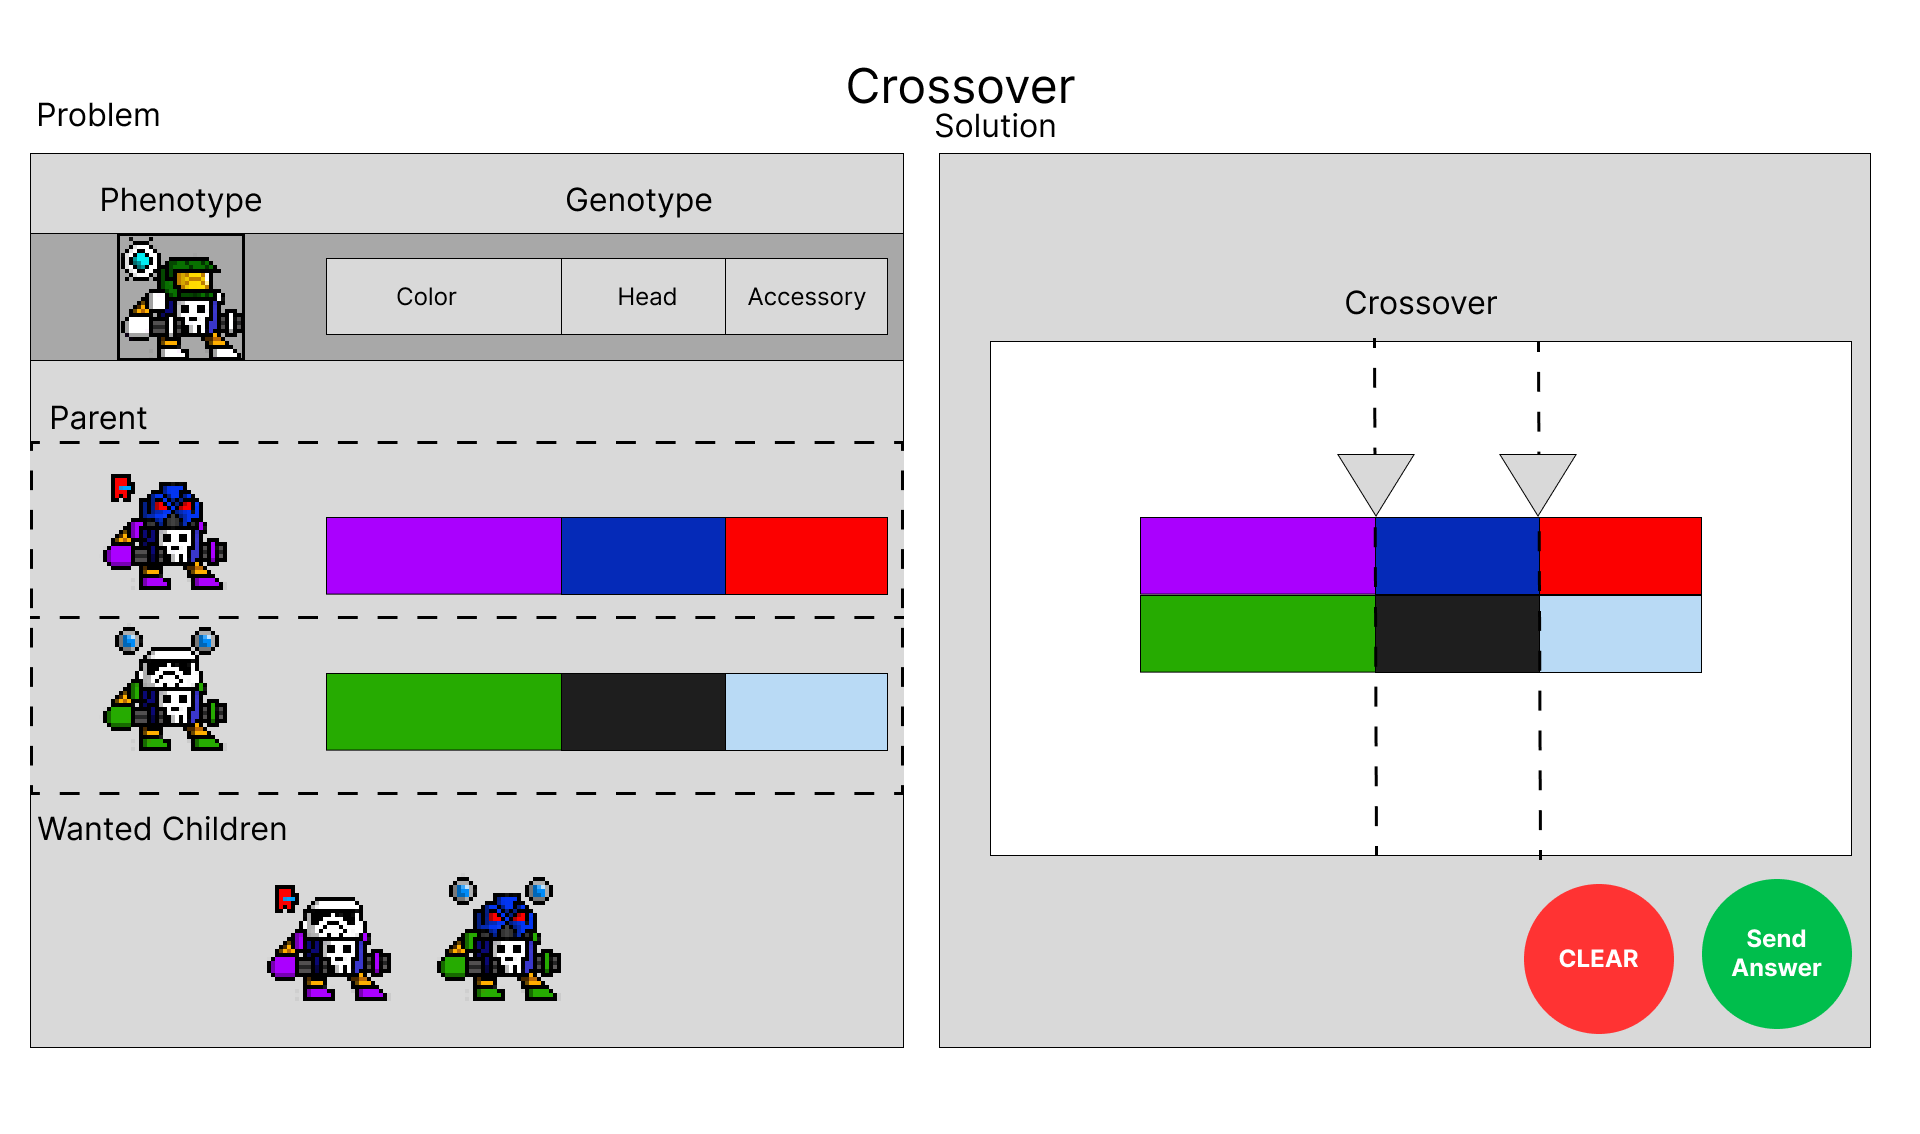
\includegraphics[width=12cm]{figure/design-puzzle-crossover.png}}
\captionof{figure}{Example of Interface of the Puzzle Gameplay}
\label{fig:design-puzzle-crossover}
\end{minipage}

Even if the main quest conducts the player continually unlocks the new facility which requires new research, the player also can enter the city freely to access other activities. Figure~\ref{fig:design-city} shows the city interface where the player can go to the quest board and receive a side quest, buy a new monster from a shop, and battle in the arena using their own monster.

%Besides the puzzle gameplay involving the research lab, monster farm and weapon factory, the player can go to the city to receive the quest, buy a new monster or the weapon chromosome, and battle in the arena using their own monster. Figure~\ref{fig:design-city} shows an example of the city interface; the players can click on the “Quest” island to go to the quest board scene in Figure~\ref{fig:design-questboard-interface-accept}, click on the “Shop” island to go to the shop scene in Figure~\ref{fig:design-shop-monster} or click on the “Arena” island to go to the arena scene and start the battle in Figure~\ref{fig:design-arena-battle} .

\begin{minipage}[c]{\textwidth}\centering
\fbox{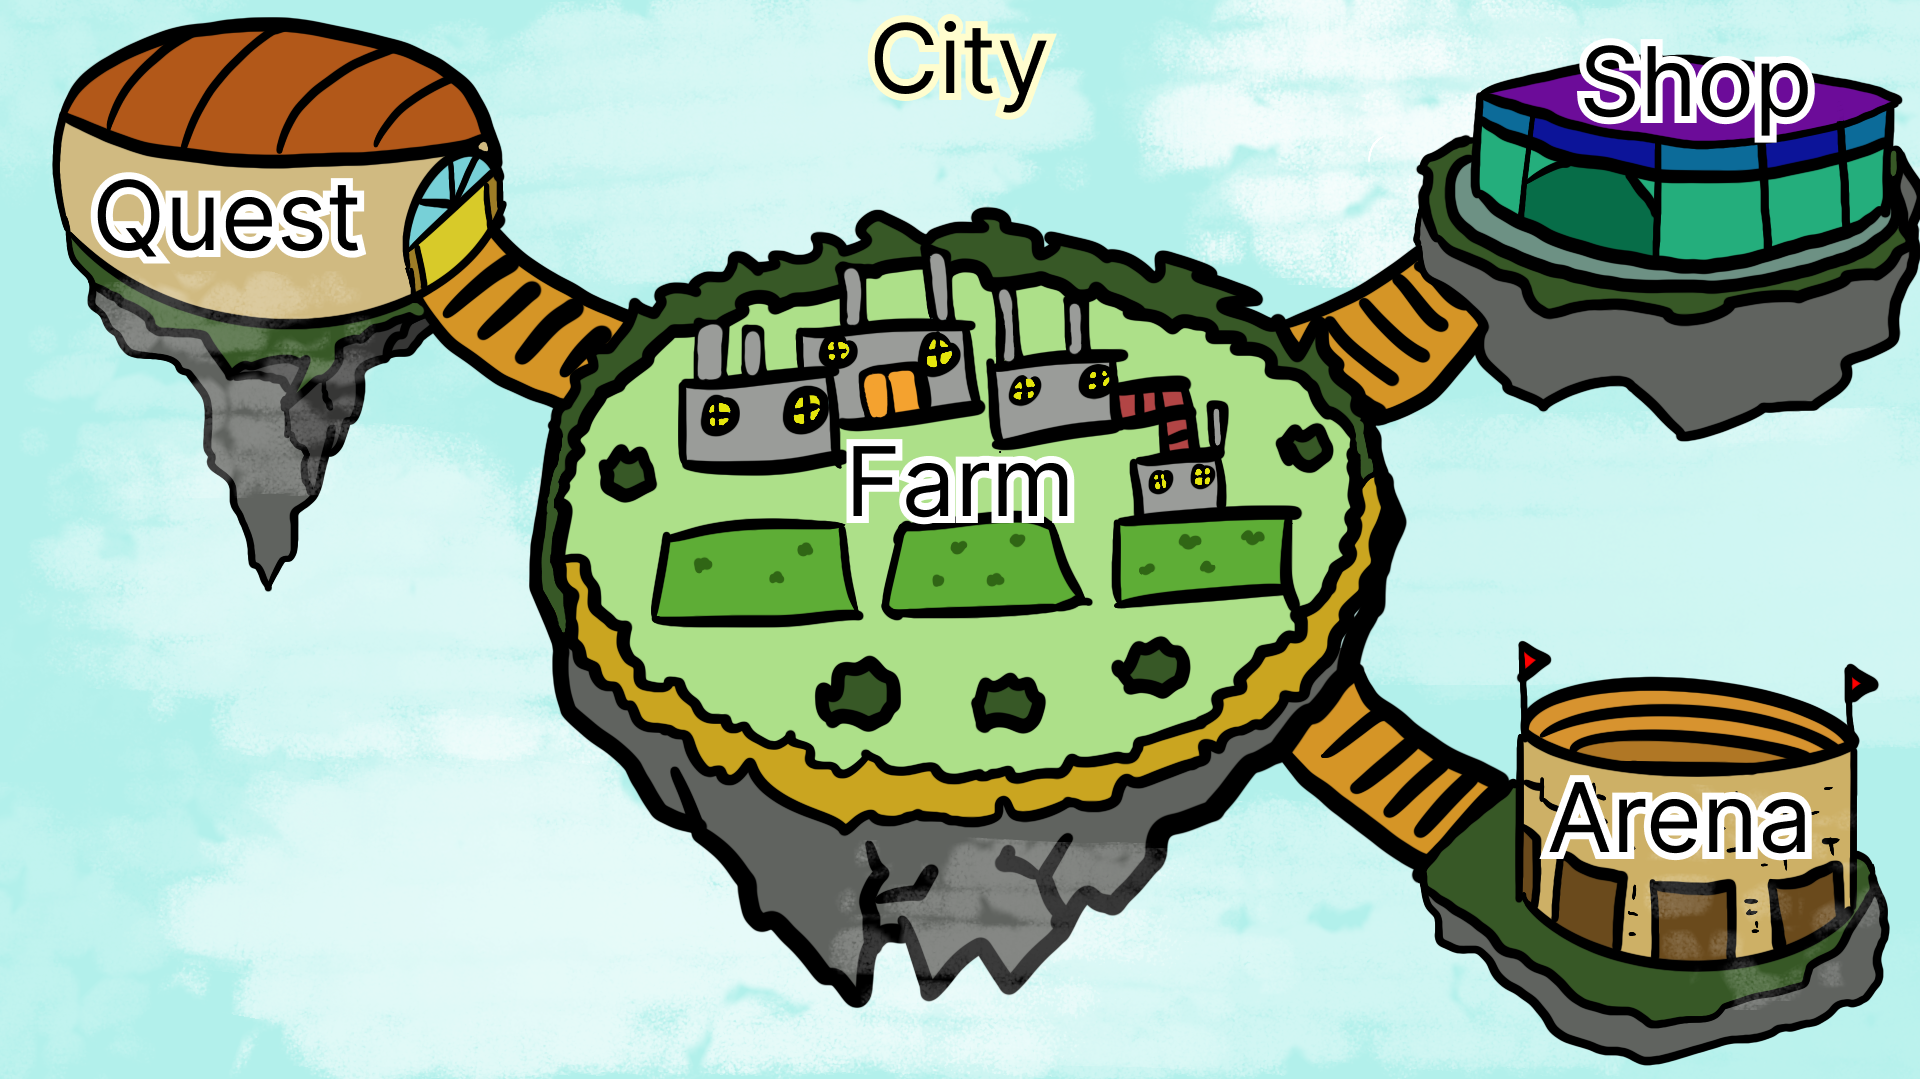
\includegraphics[width=12cm]{figure/design-city.png}}
\captionof{figure}{City Interface}
\label{fig:design-city}
\end{minipage}

When the game progresses to the late game, the last condition to indicate whether the player wins the game is the main quest that requires the player to unlock all the factories. Since the player is required to pass a skill-checking before unlocking a new factory, the player will be considered as completing the game as well as the learning outcomes upon completing the last main quest. And the player is allowed to continue playing in other systems freely without any restriction.

%When the game progresses to the late game, the last condition to indicate whether the player wins the game is the main quest that requires the player to deliver a very good weapon from every factory. If the player completes the main quest in time, the player wins the game. Otherwise, the player loses.

\end{itemize}

%%%%%%%%%%%%%%%%%%%%%%%%%%%%%%%%%%%%%%%%%%%%%%%%%%%%%%%%%%%%%%%%%%
\subsection{Gameplay and Mechanics}
Within this topic, the gameplay, main mechanics, and the replaying and saving system of our game will be explained.

\begin{itemize}
\item Gameplay \\
In this topic, we will describe how we progress the game and what the structure of both the mission and the puzzle is like.
	\begin{enumerate}
	\item Game Progression \\
	In this game, players will be played as a company owner who participates in Project-G, a global-guardian project for creating a powerful combat force for future fighting with the alien. As the game progresses, players will have to manufacture weapons in their respective factories for the government to use. \\
	In the beginning, players will start with a brand new company, so they have to unlock new facilities (monster farms and weapon factories) by themselves. To do that, they must satisfy specific requirements, such as passing a skill check for certain subjects about genetic algorithms, having enough resources, and building prior facilities. \\
	Building new factories requires money, so players also have to gather those by fulfilling requests from others or battling in the arena. To finish a request, they have to submit a monster from their company, resulting in a reduction in the overall population, which can be solved by buying new ones from the shop. \\
	After all the factories are unlocked, the game story ends since all combat power against aliens is already prepared, and the player is evaluated as completing learning as well. The minimum requirement for unlocking all factories is passing a skill check for performance level 3 for all criteria described in Table~\ref{tbl:rubric}, which is determined as a minimum level to pass the education. The player also be able to play the game furthermore without any restrictions.

	\item Mission Structure \\
	There are two types of missions in this game, main quest and side quest. Main quests will help players progress the game, and side quests will provide players with money and resources to maintain their facilities. \\
	Players are given one main quest at a time as a guideline to tell players what they could do next, such as unlocking new facilities, learning new topics, or gaining some specific resources. \\
	Side quests are requests from various sources ordering products from players' companies. The reward quality depends on how the submitted product resembles the requirement of that order. If players cannot finish the request within a time limit, that side quest will fail, and players will receive a penalty in money.
	\end{enumerate}

\item System Details \\
	The game systems can be described as states of the game. The states of the game and its transition are shown in Figure~\ref{fig:design-state-diagram} below.

\begin{minipage}[c]{\textwidth}\centering
\fbox{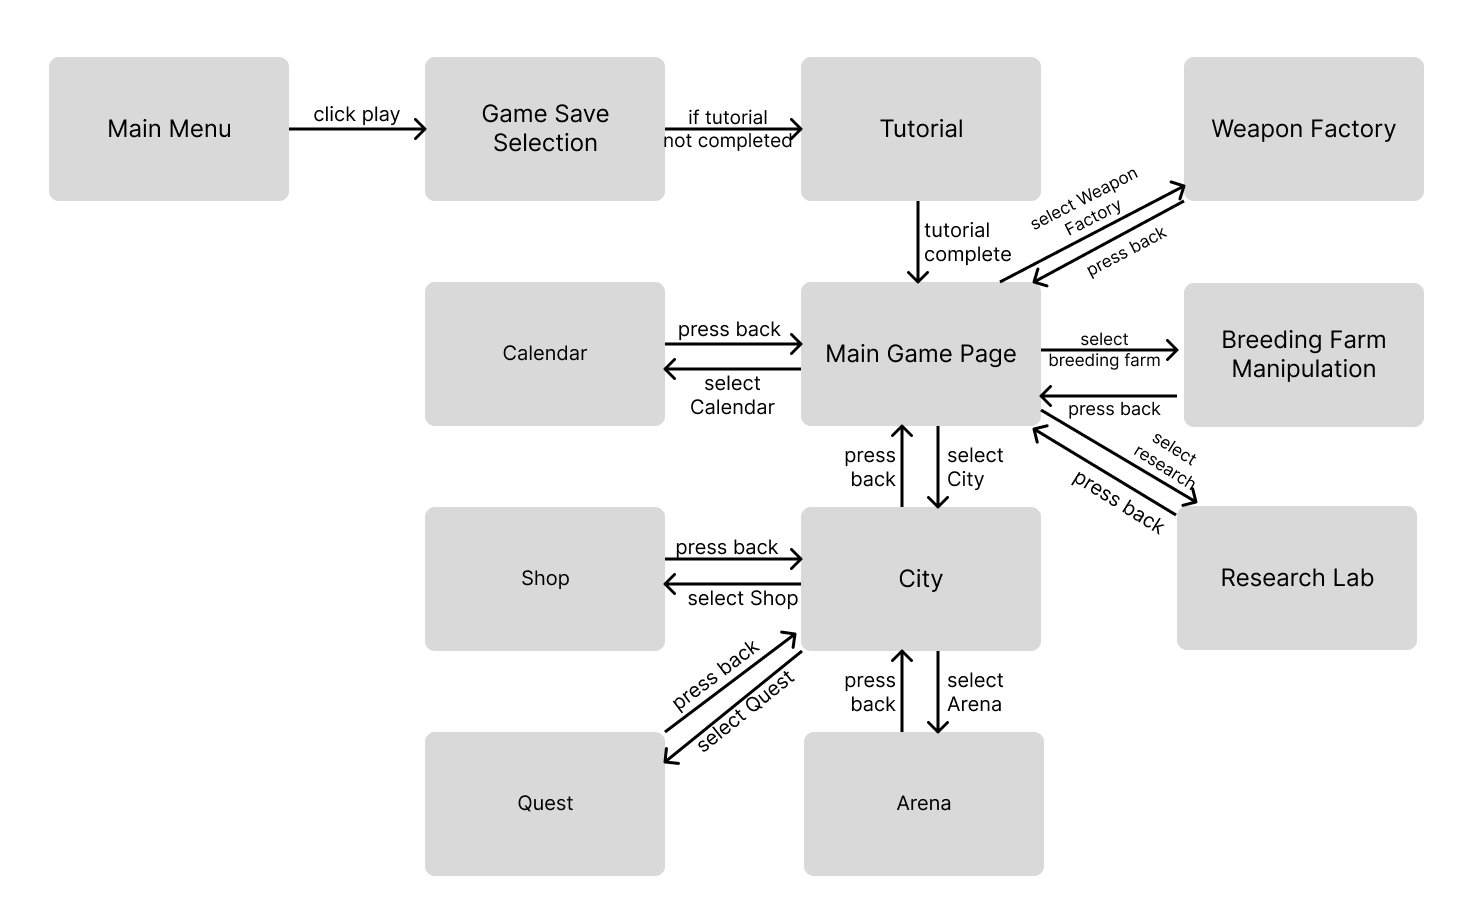
\includegraphics[width=14cm]{figure/design-state-diagram.png}}
\captionof{figure}{Overall Game State Diagram}
\label{fig:design-state-diagram}
\end{minipage}

	\begin{itemize}
	\item Main Systems \\
	These features are used for teaching and testing the players' knowledge based on the assessment criteria and level described in Table~\ref{tbl:rubric} mentioned earlier.
		
		\begin{enumerate}
		\item Cutscence \\
		This system is designed to guide players in performing specific tasks to learn how to play the game and progress through its story. Cutscenes serve another purpose by teaching players and testing their knowledge of the lessons that were taught. Cutscenes can prompt players for answers through dialogue choices and evaluate their responses to determine whether they pass the test or not.

		\item Research Lab \\
		This system allows players to learn about the Genetic Algorithm and how to solve real-world problems using it. After finishing the learning on a specific subject through the cutscene, the summary of the content will be kept in the research lab for review in the future.
		This is a system where players can learn about the Genetic Algorithm and how to solve Real World Problems with the Genetic Algorithm. The player must pass a requirement on a specific topic to unlock the particular customization in their breeding farm, such as a roulette wheel selection.\\
		All the categories, learning topics, and learning content in the research lab are based on the OBE education design and will be shown in Table~\ref{tbl:content-research-lab}.

% Please add the following required packages to your document preamble:
% \usepackage{multirow}
% \usepackage{longtable}
% Note: It may be necessary to compile the document several times to get a multi-page table to line up properly
\begin{longtable}{|l|l|l|}
\caption{The Category, Topic, and Content in Research Lab System}
\label{tbl:content-research-lab}\\
\hline
\multicolumn{1}{|c|}{Category} &
  \multicolumn{1}{c|}{Topic} &
  \multicolumn{1}{c|}{Content} \\ \hline
\endhead
%
\multirow{2}{*}{Basic Biology} &
  On the Origin of Species &
  \begin{tabular}[c]{@{}l@{}}The basic concept of Evolution and \\ Natural Selection based on Darwin’s theory.\end{tabular} \\ \cline{2-3} 
 &
  The Genetic &
  \begin{tabular}[c]{@{}l@{}}The explanation of the chromosome, gene, \\ phenotype, genotype, and biological crossover.\end{tabular} \\ \hline
\multirow{4}{*}{Genetic Algorithm} &
  \begin{tabular}[c]{@{}l@{}}The Flow of \\ Genetic Algorithm\end{tabular} &
  \begin{tabular}[c]{@{}l@{}}The introduction to the Genetic Algorithm, \\ the brief description of each step in the flowchart.\end{tabular} \\ \cline{2-3} 
 &
  Parent Selection &
  \begin{tabular}[c]{@{}l@{}}The process detail of the parent selection in \\ Genetic Algorithm include Random Selection, \\ Tournament-based Selection, Roulette Wheel \\ Selection, and Rank-based Selection.\end{tabular} \\ \cline{2-3} 
 &
  Crossover &
  \begin{tabular}[c]{@{}l@{}}The process detail of the crossover in Genetic \\ Algorithm include Single-point Crossover, \\ Two-point Crossover, and Uniform Crossover.\end{tabular} \\ \cline{2-3} 
 &
  \begin{tabular}[c]{@{}l@{}}Improvement \\ Techniques\end{tabular} &
  \begin{tabular}[c]{@{}l@{}}The description of the improvement techniques in \\ Genetic Algorithm include Elitism and the basic \\ variant mutation which consist of Bit Flip Mutation, \\ Flip Bit Mutation, and Boundary Mutation\end{tabular} \\ \hline
\multirow{3}{*}{Real-world Problems} &
  Standard Knapsack &
  \begin{tabular}[c]{@{}l@{}}The problem setting, goal, chromosome encoding, \\ and fitness evaluation of the Standard Knapsack  \\ Problem will be described.\end{tabular} \\ \cline{2-3} 
 &
  Multidimensional Knapsack &
  \begin{tabular}[c]{@{}l@{}}The problem setting, goal, chromosome encoding, \\ and fitness evaluation of the Multidimensional \\ Knapsack Problem will be described.\end{tabular} \\ \cline{2-3}
 &
  Multiple Knapsack &
  \begin{tabular}[c]{@{}l@{}}The problem setting, goal, chromosome encoding, \\ and fitness evaluation of the Multiple Knapsack \\ Problem will be described.\end{tabular} \\ \hline
\end{longtable}

		\item Hall of Intelligence \\
		This system is an extension of the Research Lab mentioned earlier. The Hall of Intelligence provides a platform for players to test their knowledge acquired from the learning materials in the Research Lab and demonstrate their learning progress. Additionally, the Hall of Intelligence tracks players' game duration, current quest status, and the number of times they have played the puzzles or tests.

		\item Assessment Methods \\
		This is a system of tests that players are required to pass to keep progressing through the game. The assessment methods for the players based on the performance descriptors outlined in Table~\ref{tbl:rubric} can be categorized as multiple-choice questions and puzzles. \\
		Multiple-choice questions utilize the cutscene system mentioned earlier to evaluate how well players can explain and classify their knowledge. The test consists of a series of multiple-choice questions, where players need to choose from dialogue choices to provide their answers. The total scores are calculated based on all the answers given, and if players achieve passing marks, they successfully clear the test. However, if they do not meet the passing marks, they will fail the test. \\
		The puzzles test is designed to assess players' knowledge acquired from the lessons by allowing them to demonstrate the step from the lesson or solve the problem related to each lesson's topic. Each topic has its own platform with specific puzzles. The puzzle platform consists of Parent Selection Puzzle, Crossover Puzzle, and Knapsack Formulation Puzzle.
		\end{enumerate}
	
	\item Primary Supporting Systems \\
	The systems include a monster farm and weapon factory where the player should use a portion of knowledge to play with. These systems are used to control the game progression using main quests since they are gameplay added to directly reinforce the will for learning of the player.
	
		\begin{enumerate}
		\item Monster Farm \\
		This is a Genetic Algorithm simulation for monster reproduction in farms. The individual monster will be encoded as a chromosome consisting of 2 sections of a gene as shown in Figure~\ref{fig:design-monster-chromosome}, each section representing each aspect of a monster including an appearance and battle status. The appearance is their head type, body color, and accessory type. The battle status includes attack, defense, health points, and speed. \\
		\begin{minipage}[c]{\textwidth}\centering
		\fbox{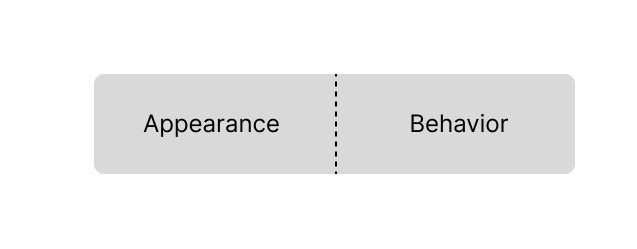
\includegraphics[width=7cm]{figure/design-monster-chromosome.png}}
		\captionof{figure}{Chromosome Representation of the Monster}
		\label{fig:design-monster-chromosome}
		\end{minipage}
		Players can adjust several parameters involved in the algorithm, such as the parent selection and crossover method. In addition to the basic operations of the Genetic Algorithm, players can utilize elitism, allowing them to preserve their favorite monster's chromosome for the next generation. The number of monsters on a farm and the number of breeding generations affect the amount of currency consumed which introduces the management gameplay into a game. Such currency is acquired from the main quest completion and other activities like a battle in the arena or capturing Capybara. Figure~\ref{fig:design-farm-interface} shows the interface of the breeding farm. The players can configure the generic algorithm of the farm in the setting on the right side and set the number of generations of breeding before starting the process by paying the total money. The player can look at the monster set in the habitat or look at the monster's detail. \\
		\begin{minipage}[c]{\textwidth}\centering
		\fbox{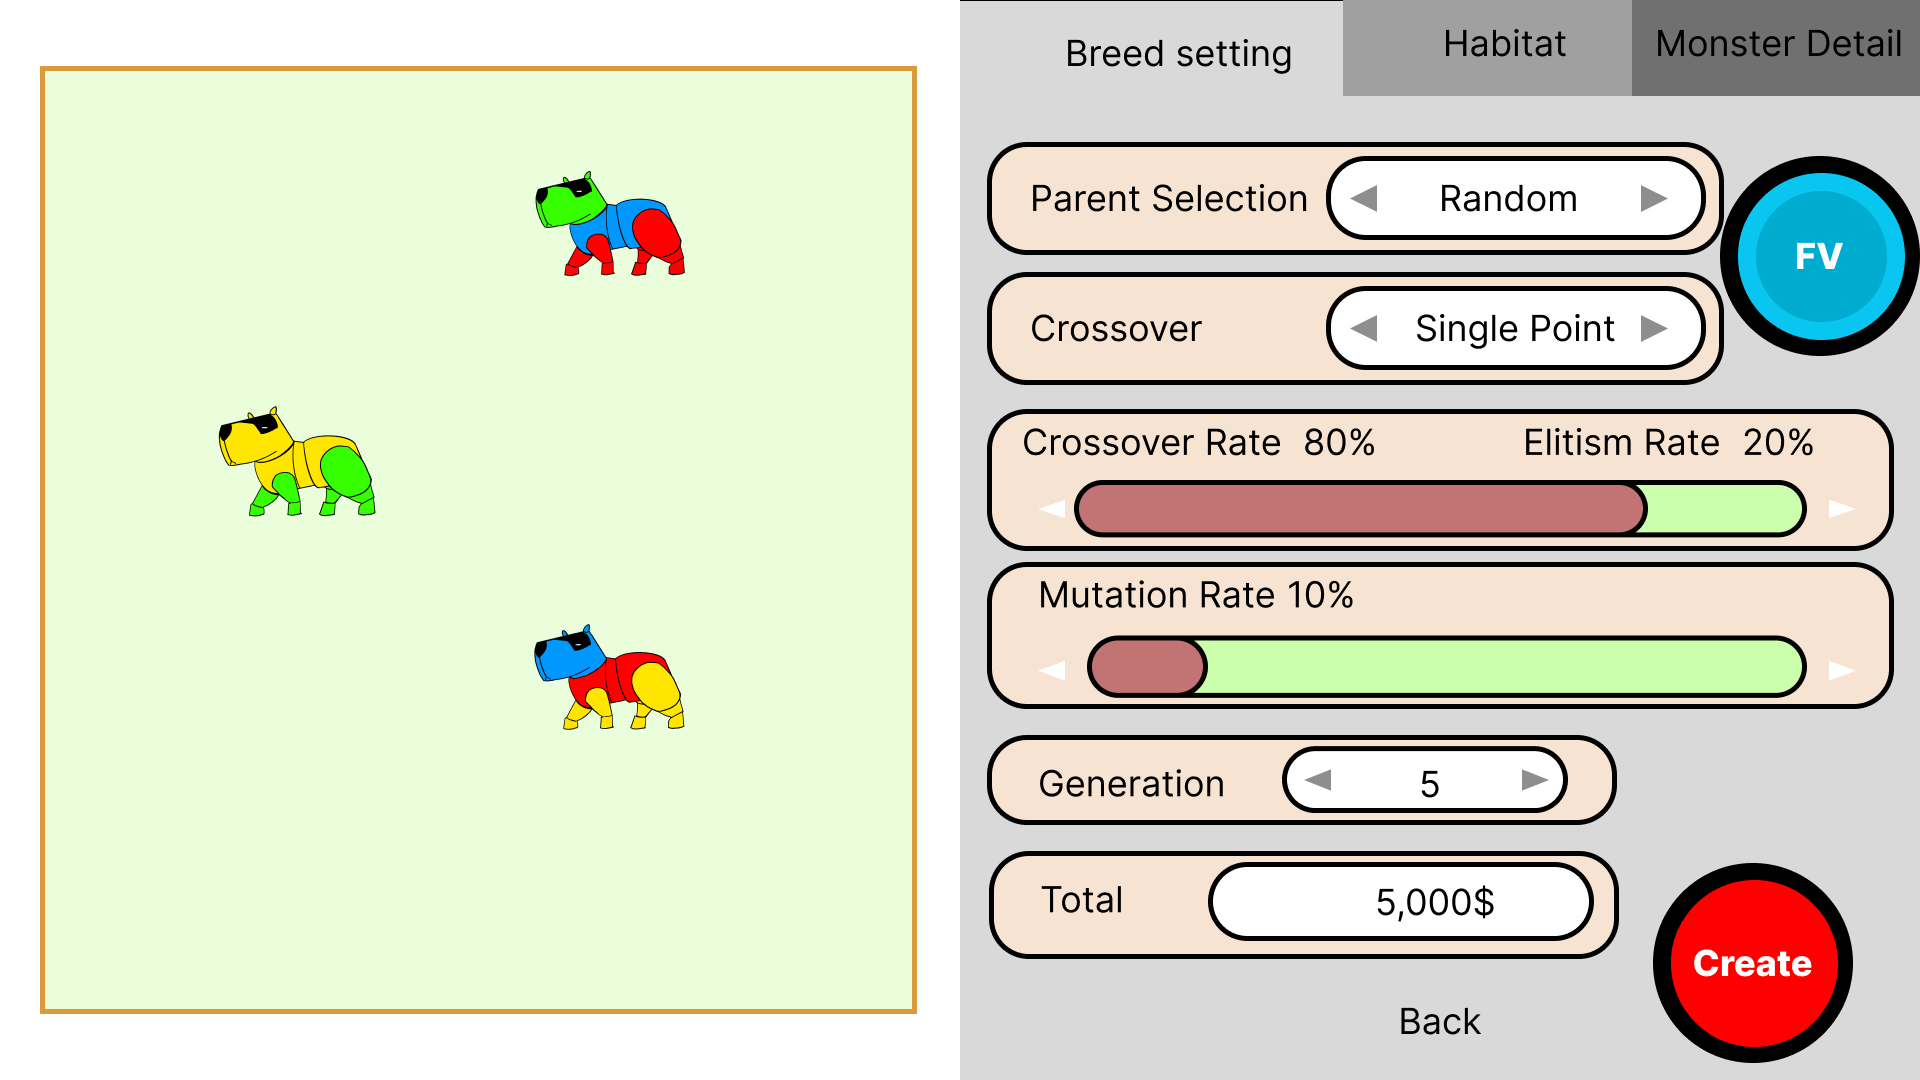
\includegraphics[width=12cm]{figure/design-farm-interface.png}}
		\captionof{figure}{Breeding Farm Interface}
		\label{fig:design-farm-interface}
		\end{minipage}

		\item Weapon Factory \\
		This system allows players to test their skills in solving real-world problems using the Genetic Algorithm. The weapons obtained from the factory are the result of attempts to solve the knapsack problem. The fitness values of each weapon's solution determine its effectiveness and appearance. These weapons can enhance the battle status of monsters, making them stronger in combat within the arena, and provide unique bonus effects specific to each factory's weapon type.
		\end{enumerate}
	
	\item Secondary Supporting Systems \\
	This is a set of systems that don't require any knowledge or skill to play with. The systems include a battle arena, side quest, and shop, which involve using their weapon and monsters in some way. The Capybara system will randomly spawn a Capybara for the player to capture. Except for the calendar system, which is used to progress the in-game activities, all the systems reward players with the resource used for breeding.

		\begin{enumerate}
		\item Battle Arena \\
		This game provides places for players to use their bred monsters to earn more resources in order to maintain their farms and factories; one of them is the arena system. Players can create a team of three monsters equipped with weapons from the factory to battle with enemy teams. \\
		\begin{minipage}[c]{\textwidth}\centering
		\fbox{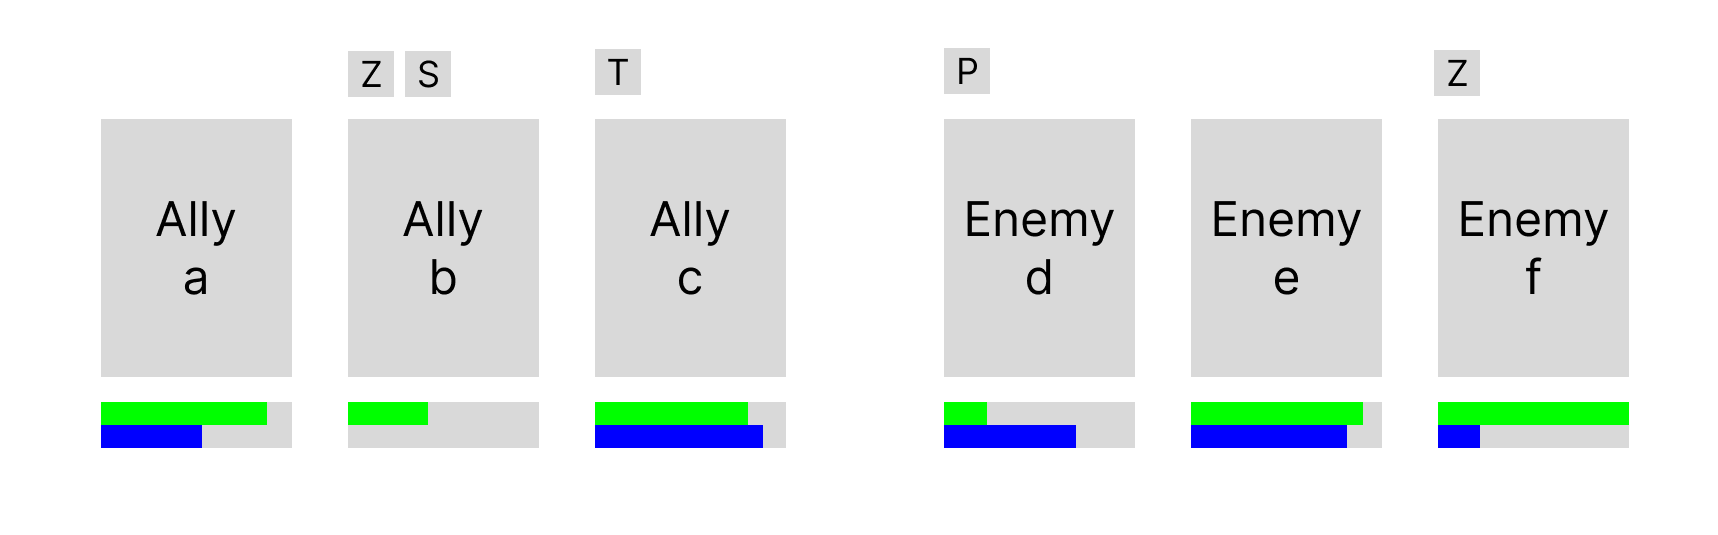
\includegraphics[width=12cm]{figure/design-arena-battle.png}}
		\captionof{figure}{Interface Design of the Battle in the Arena}
		\label{fig:design-arena-battle}
		\end{minipage}
		In Figure~\ref{fig:design-arena-battle}, the players' monster team is on the left and the enemy team is on the right side of the scene. Each monster will attack automatically after the speed gauge is filled (blue gauge). Attack targets will get chosen randomly depending on their corresponding space. If the health gauge runs out, that monster is out of combat. The battle will end when the whole team is unable to battle. There is a time limit to this combat; if time runs out but the battle does not finish, the overtime phase will begin, and every monster will get a boost for a small period of time. After the overtime phase, the team with more health will win. Finally, the reward given to players of that battle depends on the result.
	
		\item Side Quest \\
		Another system for players to gain resources is the side quest system. There are requests from various sources for players to fulfill by submitting monsters satisfying their requirements. The resemblance of those objects will affect the number of rewards directly. If players cannot accomplish quests they received within a time limit, those quests will fail. The designed interface of the side quest system is in Figure~\ref{fig:design-questboard-interface-accept} and ~\ref{fig:design-questboard-interface-submit}. \\
		\begin{minipage}[c]{\textwidth}\centering
		\fbox{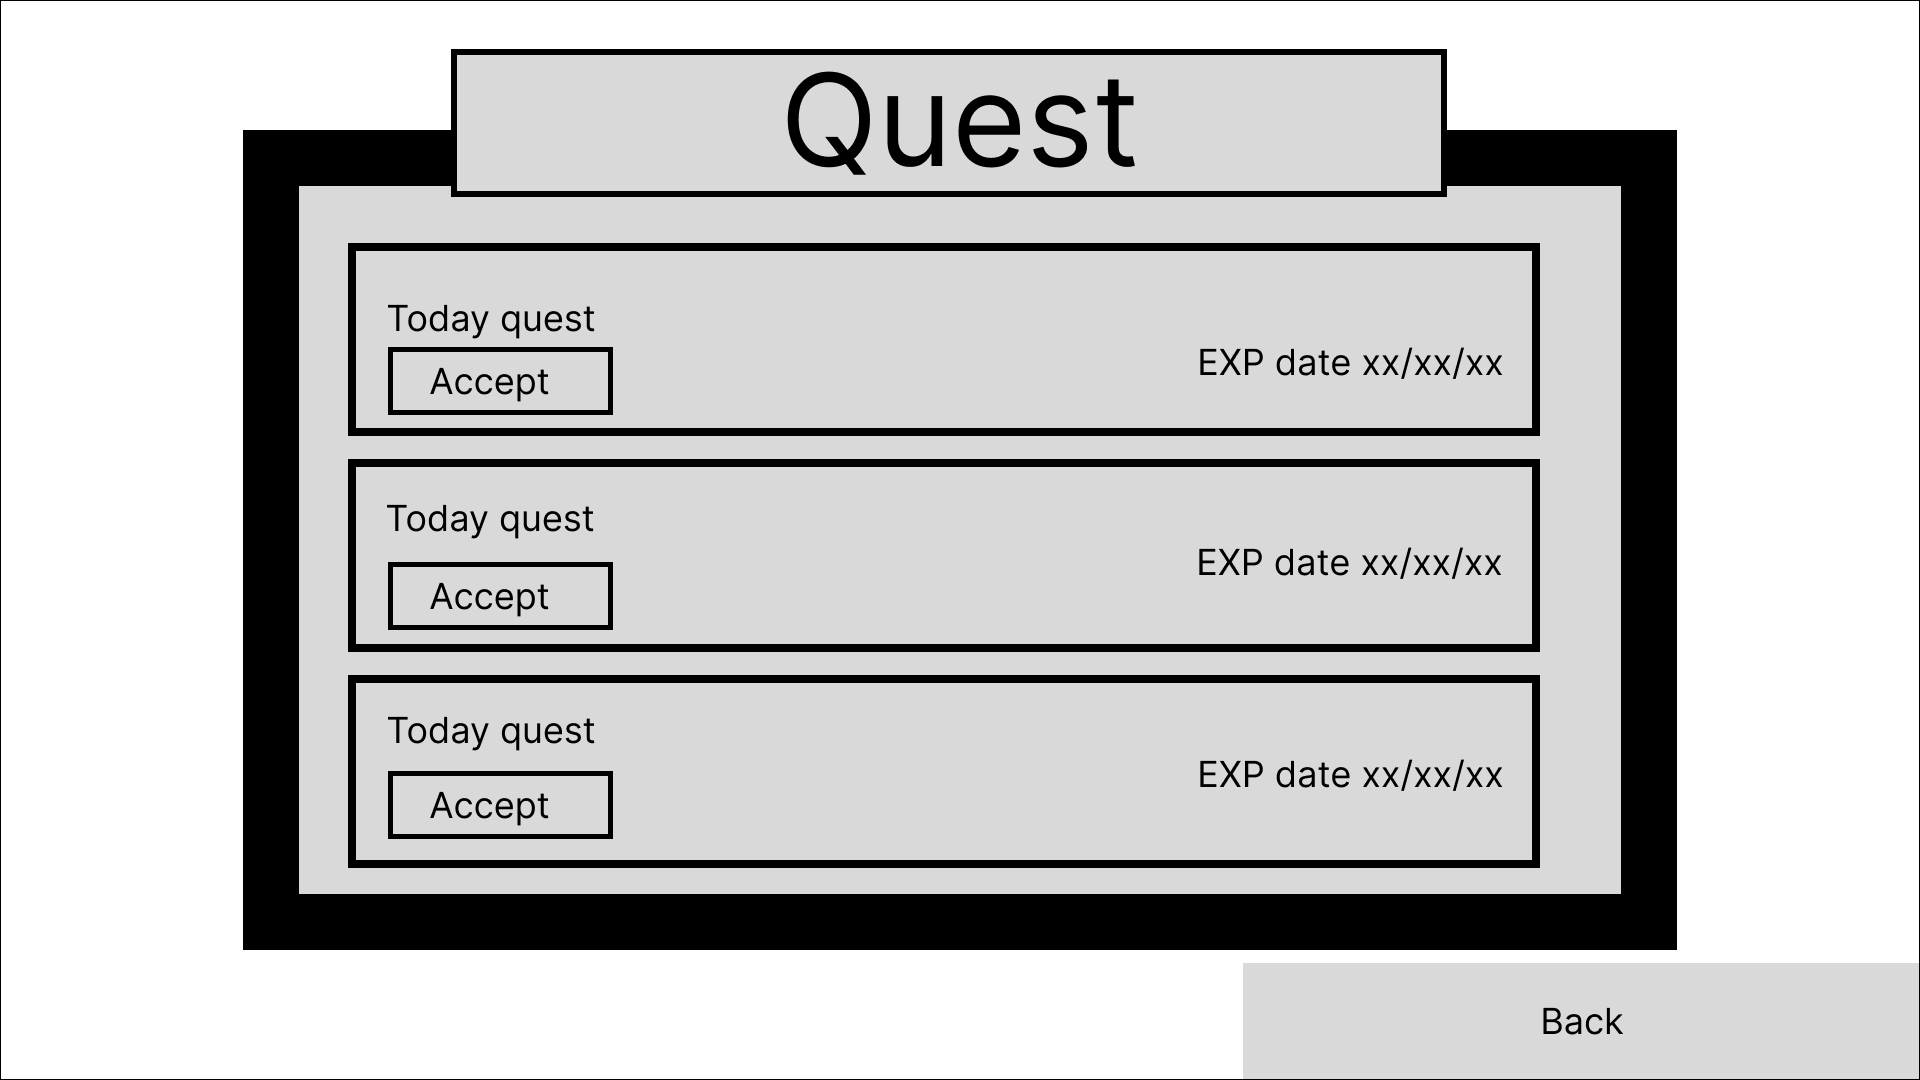
\includegraphics[width=12cm]{figure/design-questboard-interface-accept.png}}
		\captionof{figure}{Interface of Questboard for Accept Quest Scene}
		\label{fig:design-questboard-interface-accept}
		\end{minipage}
		\begin{minipage}[c]{\textwidth}\centering
		\fbox{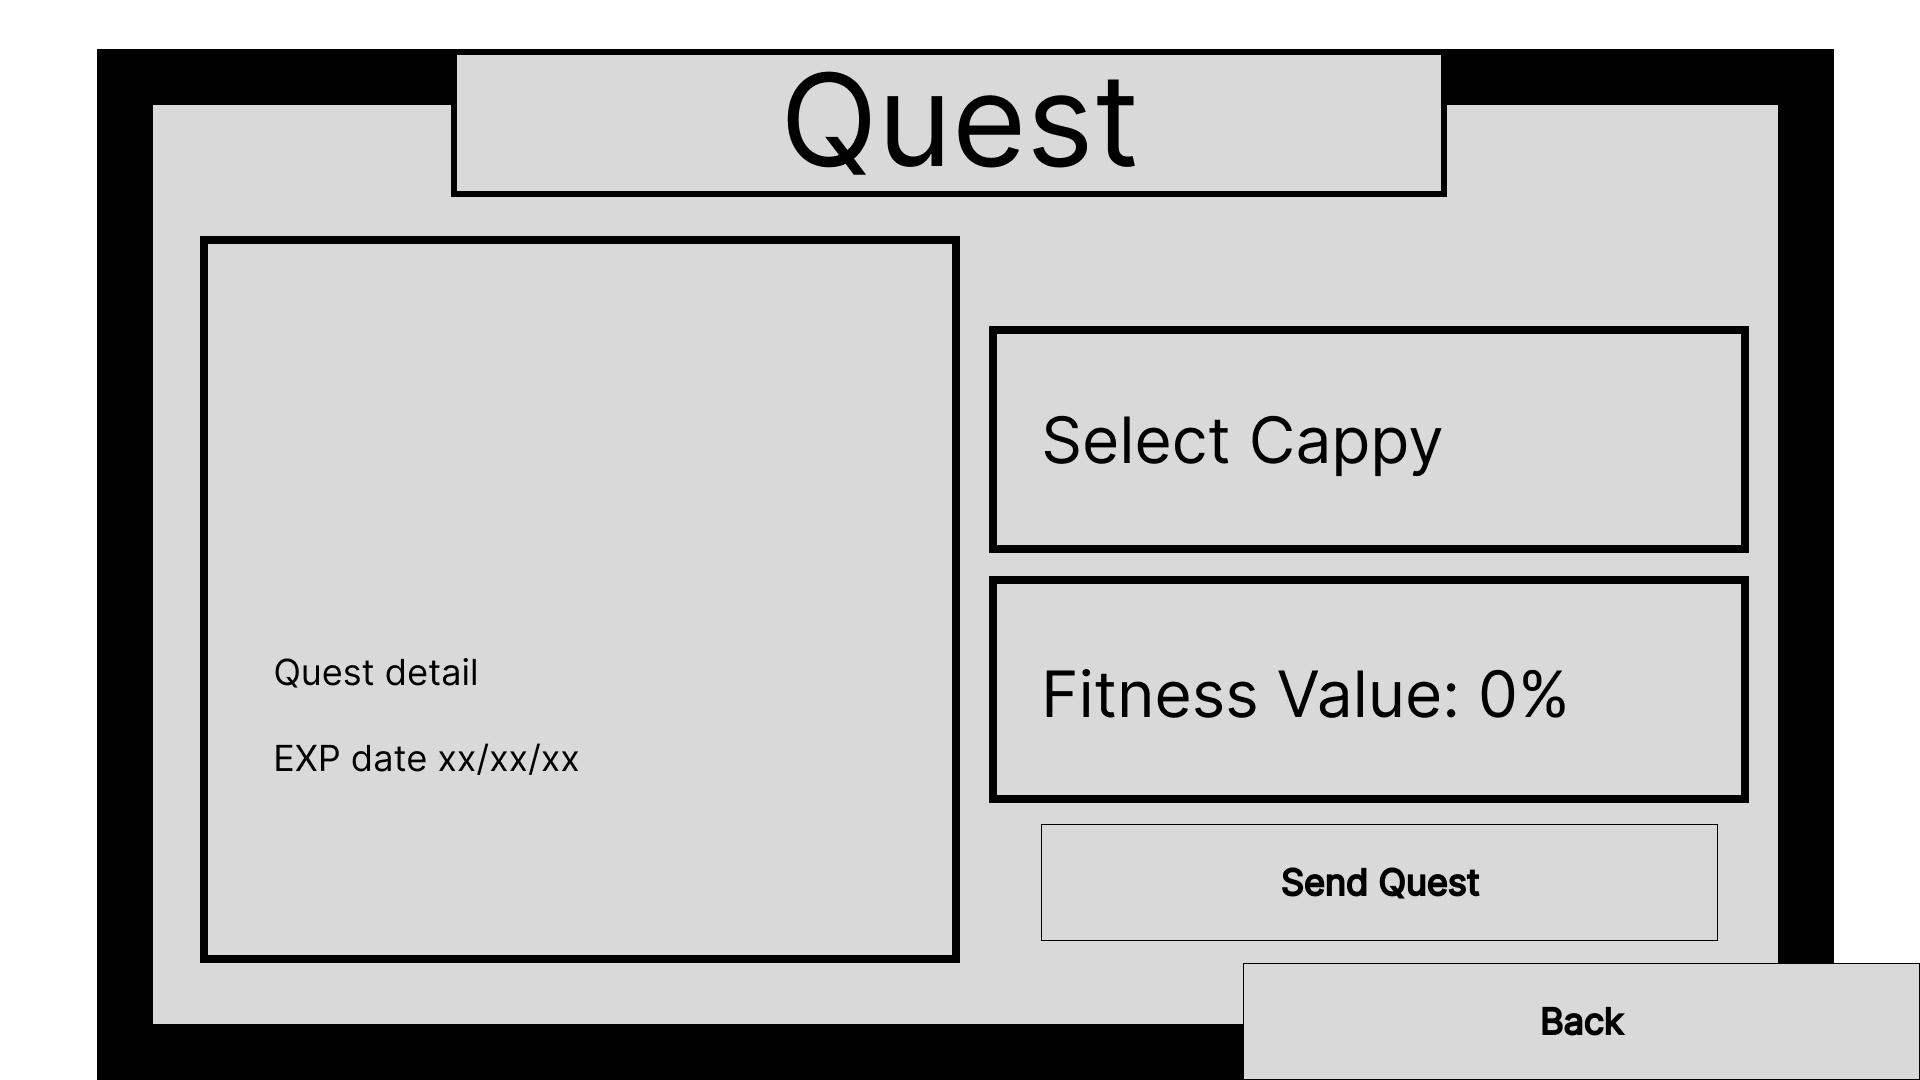
\includegraphics[width=12cm]{figure/design-questboard-interface-submit.png}}
		\captionof{figure}{Interface of Quest Submission Scene}
		\label{fig:design-questboard-interface-submit}
		\end{minipage}
		In Figure~\ref{fig:design-questboard-interface-accept}, the players can choose the quest they want to accept. The quest board will provide details of the quest including the appearance of the requested monster and time limit of the quest. If the players accept and in Figure~\ref{fig:design-questboard-interface-submit}, the players can submit their monster to complete the quest.
	
		\item Shop \\
		After submitting quests, the population of monsters will decrease, and players could buy new ones from the shop to regain the population. The shop will refresh weekly with a new batch of randomized products for players to buy with money. The example of the designed interface of the shop page is shown as Figure~\ref{fig:design-shop-monster}. \\
	%	\begin{minipage}[c]{\textwidth}\centering
	%	\fbox{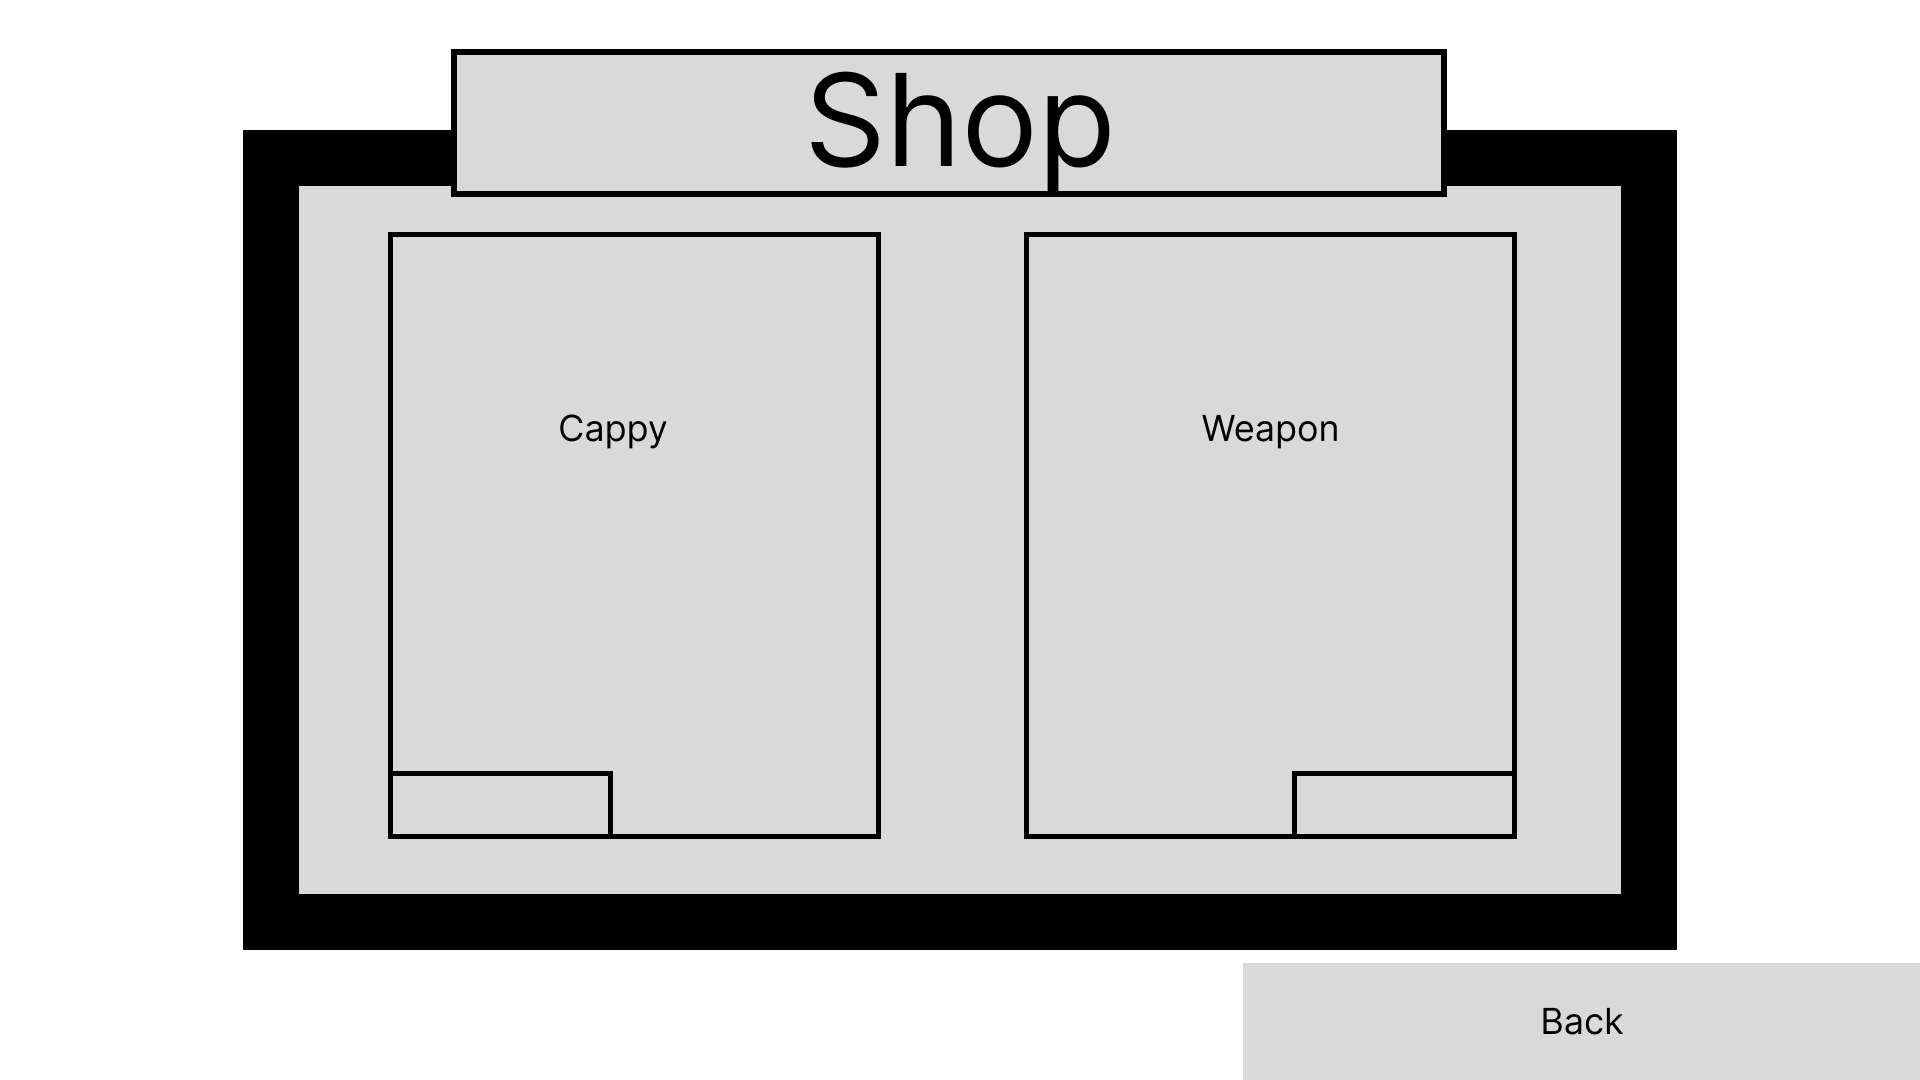
\includegraphics[width=12cm]{figure/design-shop-main-inteface.png}}
	%	\captionof{figure}{Interface of Main Shop Page}
	%	\label{fig:design-shop-main-inteface}
	%	\end{minipage}
	%	\begin{minipage}[c]{\textwidth}\centering
	%	\fbox{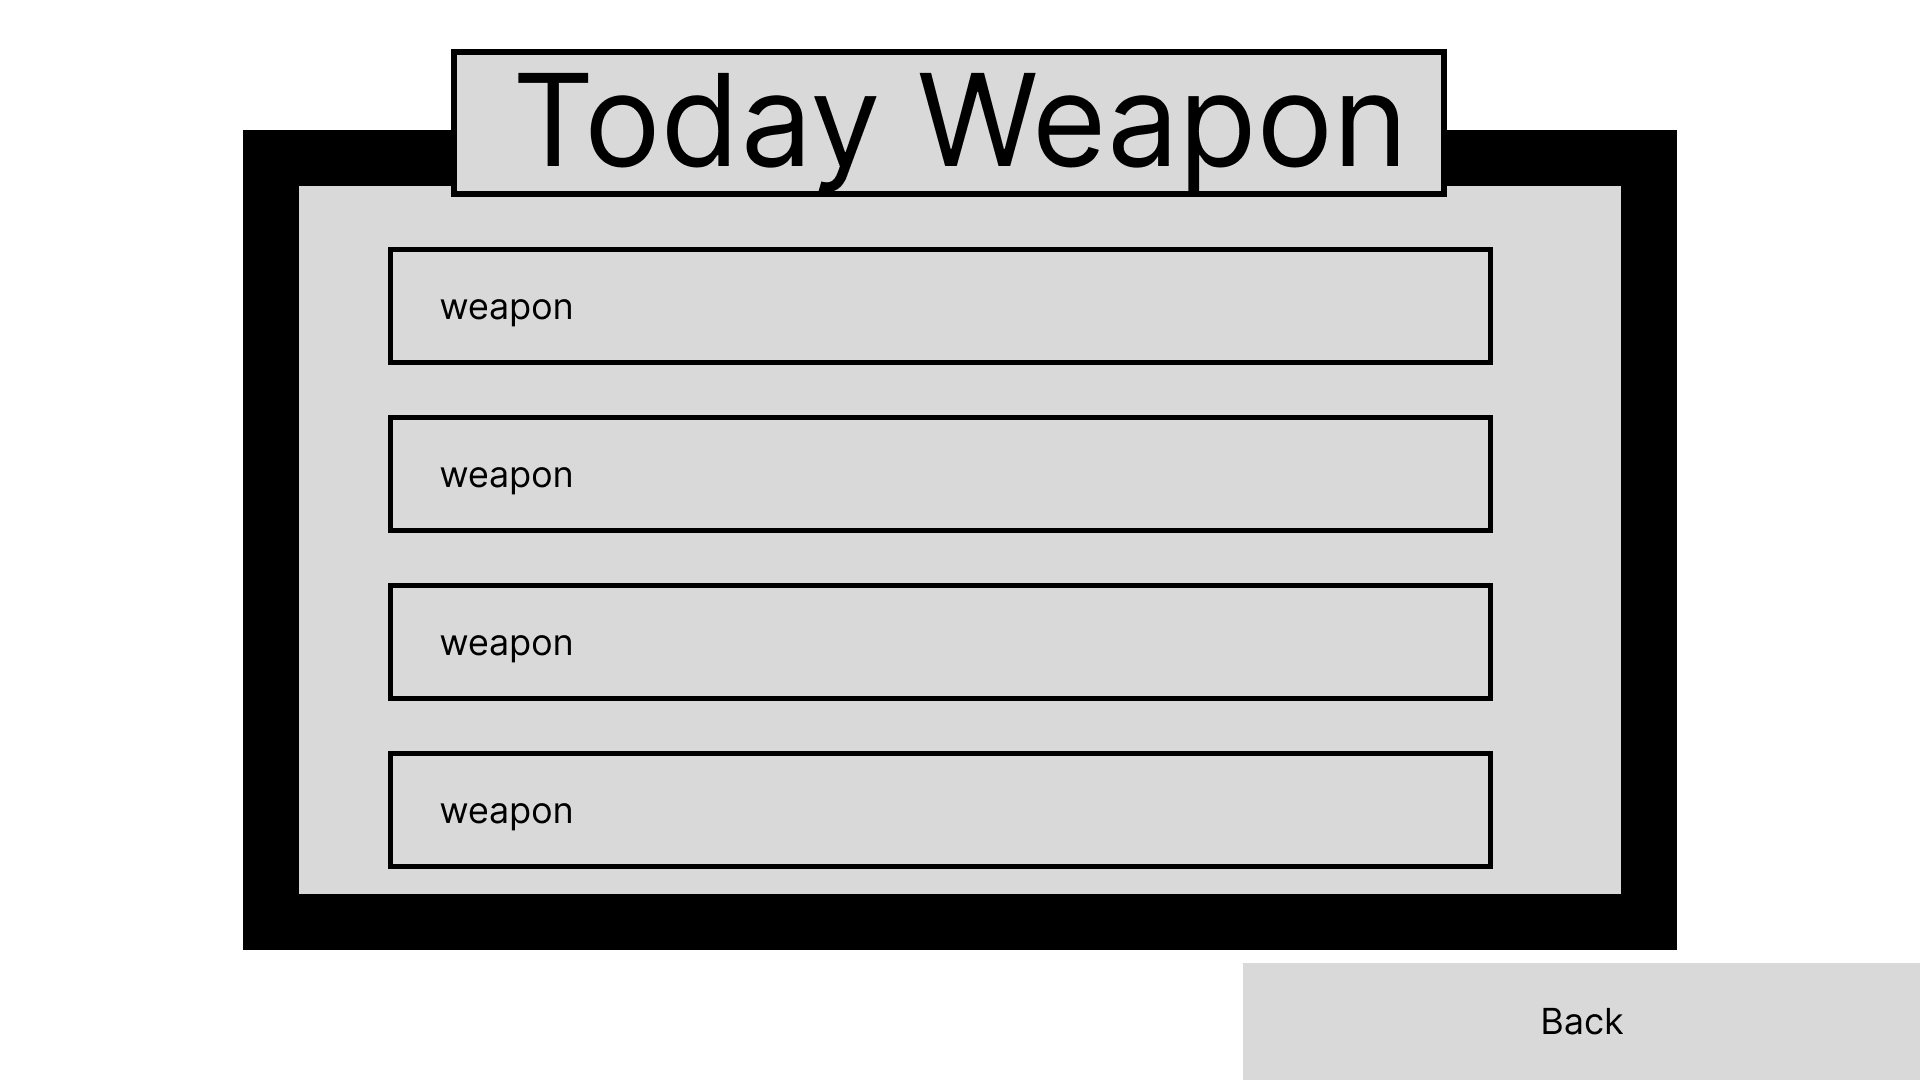
\includegraphics[width=12cm]{figure/design-shop-weapon.png}}
	%	\captionof{figure}{Interface of Weapon Shop Page}
	%	\label{fig:design-shop-weapon}
	%	\end{minipage}
		\begin{minipage}[c]{\textwidth}\centering
		\fbox{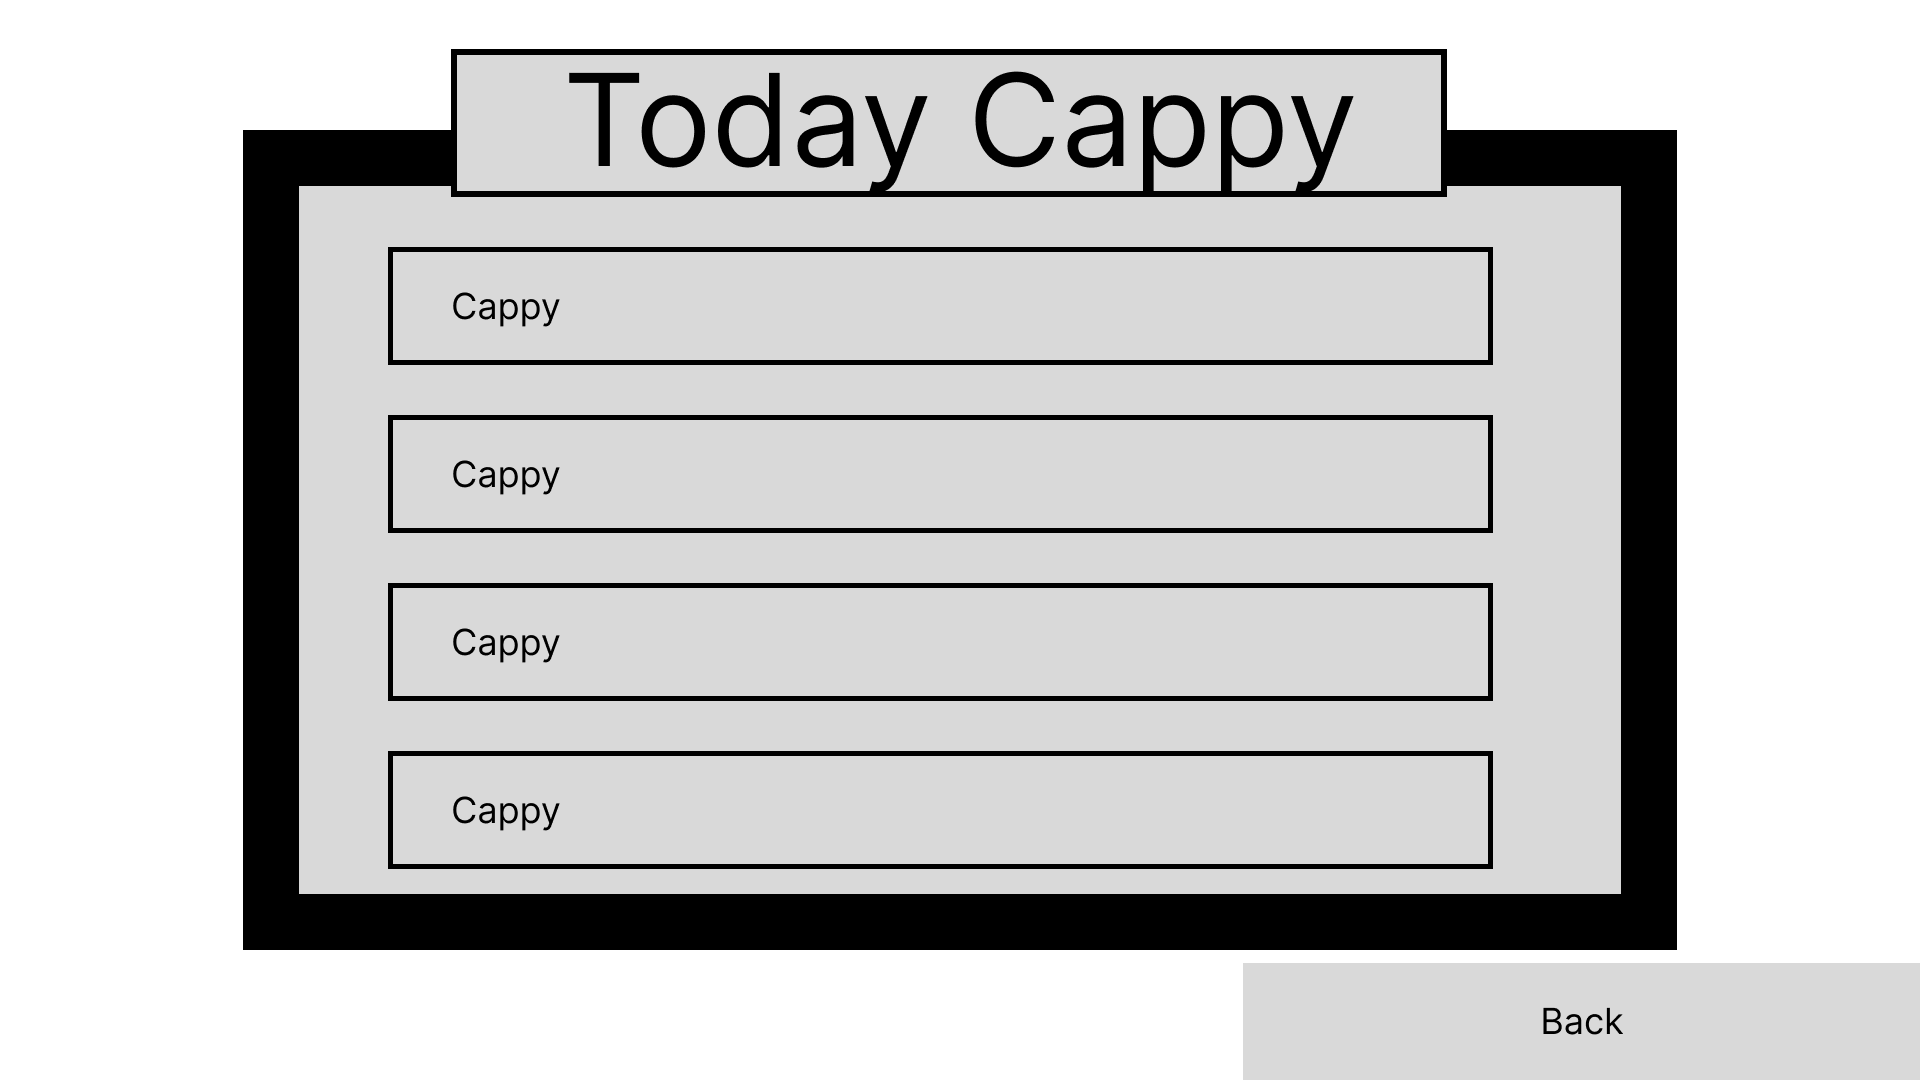
\includegraphics[width=12cm]{figure/design-shop-monster.png}}
		\captionof{figure}{Interface of the Shop Page}
		\label{fig:design-shop-monster}
		\end{minipage}

		\item Capybara \\
		This is a random event that a random species of Capybara walk by the facility on the main page. It's an addition that represents the variation in genetics using a variety in the appearance of each species. Different species hold a different number of clicks required for capture and a different amount of reward. The player can rapidly click on Capybara to capture it, and the player will get a reward upon successful capture.
		
		\item Calendar \\
		Time in this game will progress when players decide to end their day. The calendar system displays many details related to date and time, such as quest submission date, breeding completion date, and other events. The game will automatically save when players end their day, and the next day will begin. The designed interface of the calendar system is in Figures~\ref{fig:design-calendar}. \\
		\begin{minipage}[c]{\textwidth}\centering
		\fbox{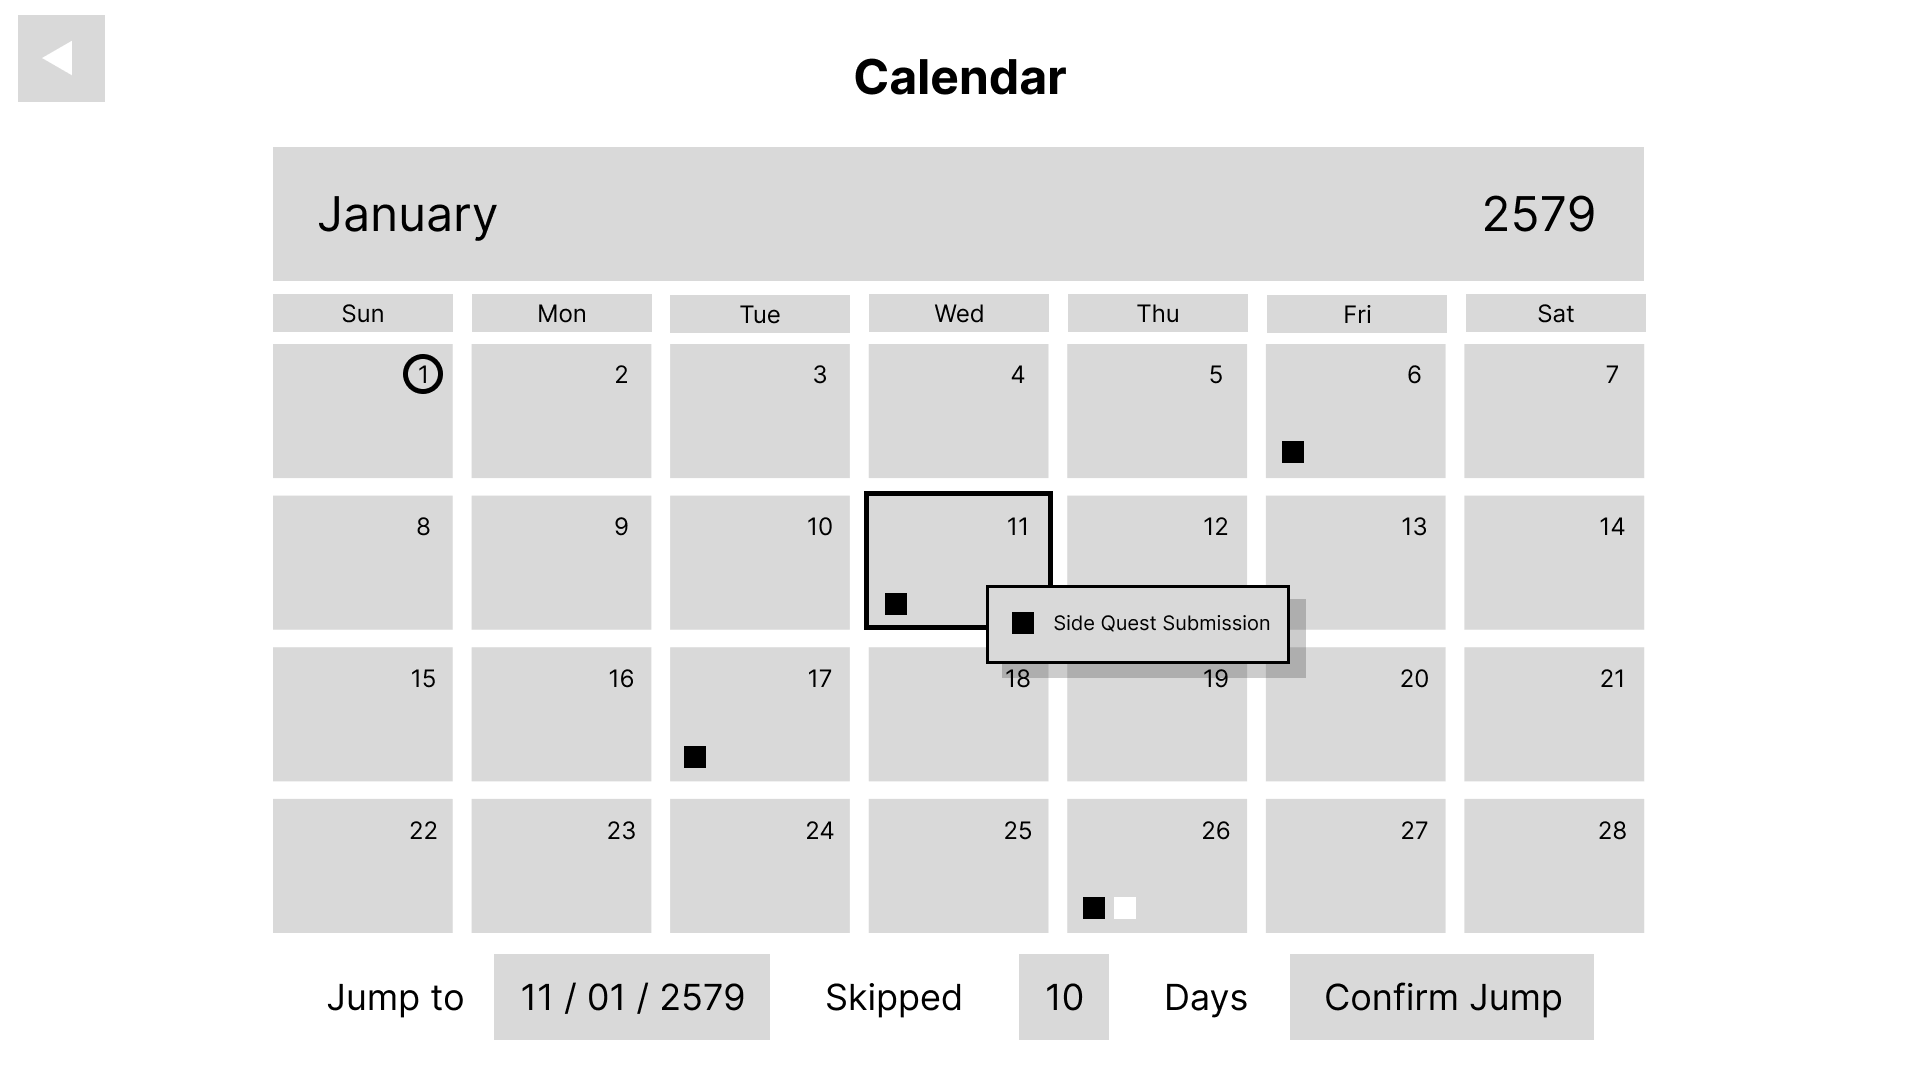
\includegraphics[width=12cm]{figure/design-calendar.png}}
		\captionof{figure}{Interface of the Calendar System}
		\label{fig:design-calendar}
		\end{minipage}
		\end{enumerate}
	\end{itemize}

	



% This is a facility unlock requirements
% Please add the following required packages to your document preamble:
% \usepackage{longtable}
% Note: It may be necessary to compile the document several times to get a multi-page table to line up properly
%\begin{longtable}{|l|l|}
%\caption{Farms Unlock Requirements}
%\label{tbl:farm-unlock-requirements}\\
%\hline
%Farm   & Unlock Requirement                                               \\ \hline
%\endhead
%%
%Farm 1 &
%  \begin{tabular}[c]{@{}l@{}}Complete Research\\ - On the Origin of Species\\ - The Genetic\\ - The Flow of Genetic Algorithm\\ - Random Selection\\ - Single-point Crossover\\ - Elitism\\ - Boundary Mutation\\ Money\end{tabular} \\ \hline
%Farm 2 & \begin{tabular}[c]{@{}l@{}}Unlock Factory 2\\ Money\end{tabular} \\ \hline
%Farm 3 & \begin{tabular}[c]{@{}l@{}}Unlock Factory 3\\ Money\end{tabular} \\ \hline
%\end{longtable}
%
%	The player must meet the requirements on the Table~\ref{tbl:farm-unlock-requirements} to unlock more Farms.
%
%	\item Weapon Factory System \\
%	This is a system where players can test themselves on how to solve Real-World Problems with the Genetic Algorithm.
%
%% Please add the following required packages to your document preamble:
%% \usepackage{longtable}
%% Note: It may be necessary to compile the document several times to get a multi-page table to line up properly
%\begin{longtable}{|l|l|}
%\caption{Weapon Factories Unlock Requirements}
%\label{tbl:factory-unlock-requirement}\\
%\hline
%\multicolumn{1}{|c|}{Weapon Factory} & \multicolumn{1}{c|}{Unlock Requirement}                                                                                             \\ \hline
%\endhead
%%
%Factory 1                            & \begin{tabular}[c]{@{}l@{}}Unlock Farm 1\\ Complete Research\\ - Standard 0/1 MKP\\ - Bit Flip Mutation\\ Money\end{tabular}        \\ \hline
%Factory 2 & \begin{tabular}[c]{@{}l@{}}Unlock Factory 1\\ Complete Research\\ - Tournament-based Selection\\ - Flip Bit Mutation\\ Money\end{tabular}                      \\ \hline
%Factory 3 & \begin{tabular}[c]{@{}l@{}}Unlock Factory 2\\ Complete Research\\ - Multiple 0/1 MKP\\ - Roulette Wheel Selection\\ - Two-point Crossover\\ Money\end{tabular} \\ \hline
%Factory 4                            & \begin{tabular}[c]{@{}l@{}}Unlock Factory 3\\ Complete Research\\ - Rank-based Selection\\ - Uniform Crossover\\ Money\end{tabular} \\ \hline
%\end{longtable}
%
%	The player must meet the requirements on the Table~\ref{tbl:factory-unlock-requirement} to unlock more factories. The factory can enhance monsters' battle status and make them stronger in battle.
%
	
	


\item Mechanics \\
Besides the mechanics described in the system detail section, the summary of the action the player can perform in our game will be described.

\begin{enumerate}
	\item Use Cases \\
	\begin{minipage}[c]{\textwidth}\centering
	\fbox{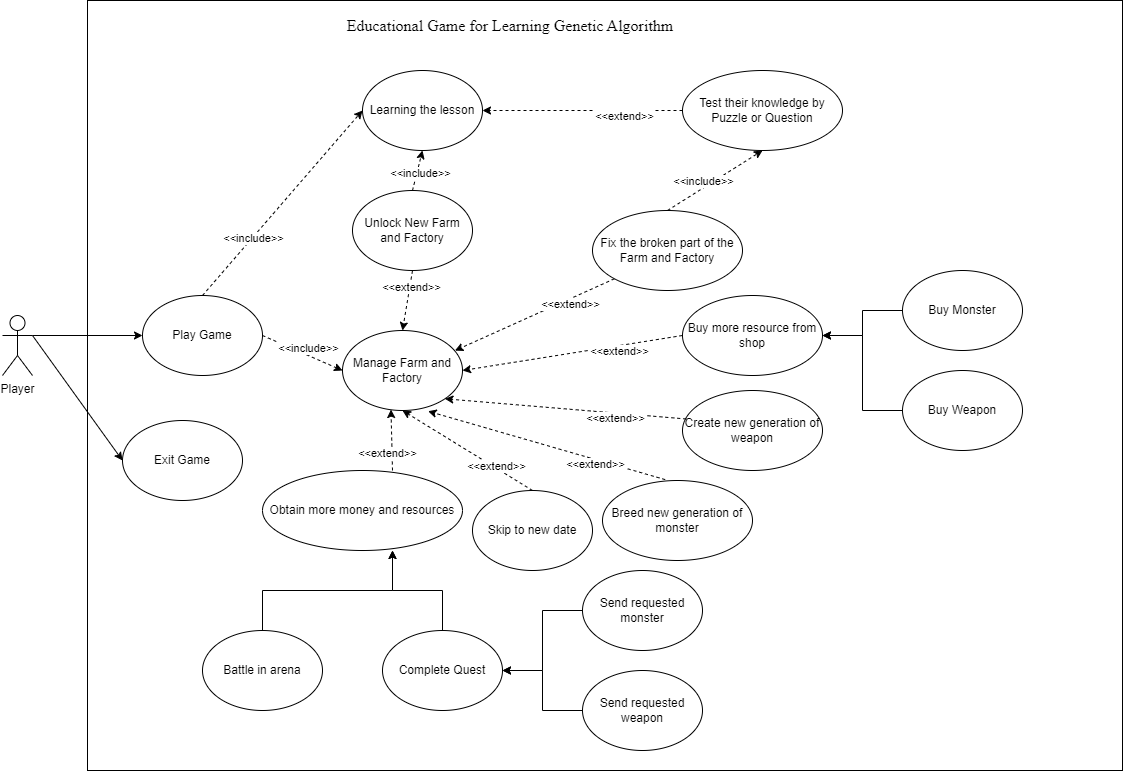
\includegraphics[width=12cm]{figure/design-usecase-diagram.png}}
	\captionof{figure}{Use Cases Diagram}
	\label{fig:design-usecase-diagram}
	\end{minipage}
	Figure~\ref{fig:design-usecase-diagram} shows the actions the player can perform in our game.Players can start playing or exit the game when starting the program. After players choose to play the game, they can learn the lesson from the research lab or managing farms and factories in the main gameplay scene. After finishing a lesson, players must take a test to evaluate their knowledge of that topic. Also, they can unlock new facilities by fulfilling some requirements such as money, resources, and learning lessons. When farms and factories break, players have to solve puzzles using knowledge of the genetic algorithm to fix the broken part. Players can breed a new generation of monsters and weapons from corresponding farms and factories using their money or resources. They can buy more monsters or weaponry from the shop to increase the population in farms and factories. Maintaining facilities requires spending resources, so players have to manage and earn more in some way. In order to do that, they can build a team of monsters equipped with weapons to battle in the arena; or satisfy requests from people ordering monsters or weapons from players' companies.

	\item Economy \\
	Money is the main resource in this game. It is used in many places, including unlocking new research and facility, breeding weapons and monsters, and purchasing new monsters. Players can earn money by completing main and side quests, winning the battle in the arena, and capturing Capybara. The unlocking fee for new research is set to be very low compared to other situations to prevent the situation that money be an obstacle to learning.
\end{enumerate}

\item Replaying and Saving \\
According to the calendar system, the game will save when players end the day and move on to the next day. Players can exit the game freely, but the game will start from the beginning of the day after the saving occurs.
\end{itemize}


%%%%%%%%%%%%%%%%%%%%%%%%%%%%%%%%%%%%%%%%%%%%%%%%%%%%%%%%%%%%%%%%%%
%%%%%%%%%%%%%%%%%%%%%%%%%%%%%%%%%%%%%%%%%%%%%%%%%%%%%%%%%%%%%%%%%%
\section{Development}
This phase of work aims to develop the learning materials and the learning activities. Such activities in the context of the educational game are precisely the puzzle gameplay that we will use as learning and assessment activities. The following content will describe the learning material, the structure of the puzzle, and prototyping and usability testing.

%%%%%%%%%%%%%%%%%%%%%%%%%%%%%%%%%%%%%%%%%%%%%%%%%%%%%%%%%%%%%%%%%%
\subsection{Learning Material}
From the expected outcome, we break it down and list the topic of the learning content as we mentioned in the research lab system. For each topic, the image and description text is created. Figure~\ref{fig:develop-learning-material-SPC} is an example of the learning material we created for the single-point crossover. Please note that the material will be adapted to suit the game dialogue later, and all the learning materials are provided in the Appendix. %~\ref{appendix:learning-material}.

\begin{figure}[!h]\centering
\fbox{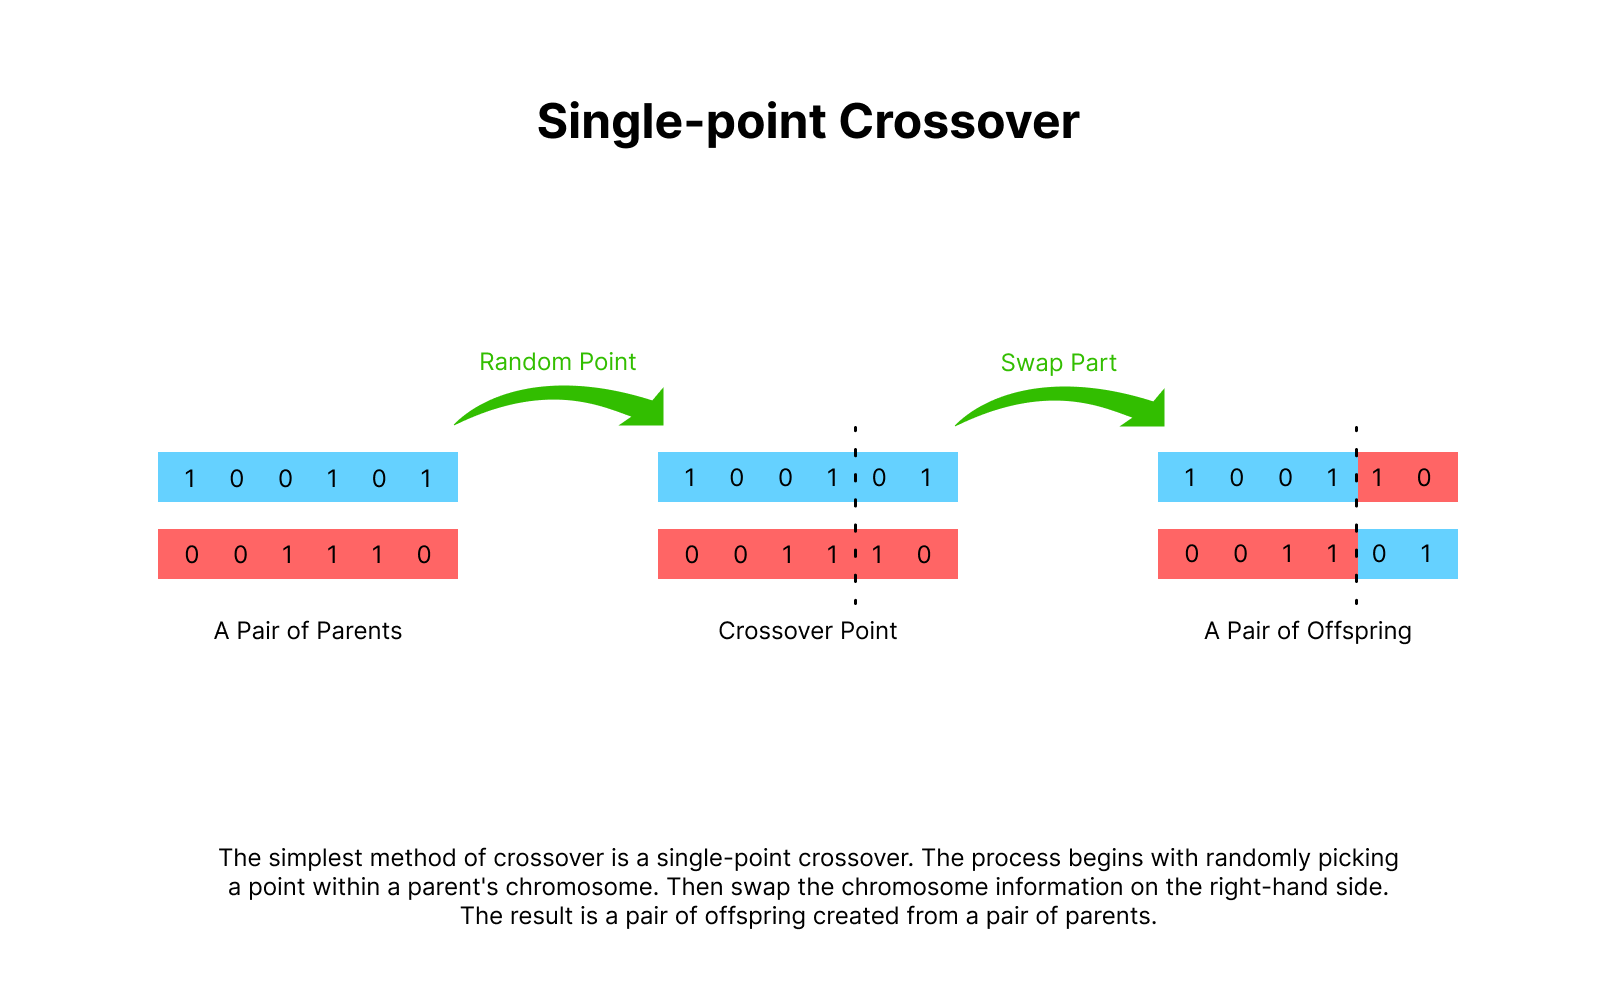
\includegraphics[width=14cm]{figure/develop-learning-material-SPC.png}}
\caption{Learning Material for Single-point Crossover.}
\label{fig:develop-learning-material-SPC}
\end{figure}

%%%%%%%%%%%%%%%%%%%%%%%%%%%%%%%%%%%%%%%%%%%%%%%%%%%%%%%%%%%%%%%%%%
\subsection{Puzzle Structure}
The puzzle will be used as an assessment activity for the demonstration and solving level of learning of the criteria in the rubric Table~\ref{tbl:rubric}. These puzzles not only will be used as an assessment but also will be used as an exercise that helps the player maintain and verify their knowledge. \\
The players will encounter puzzles in 2 different situations. The first situation is right after the players finish learning the lesson from the research lab. The players are required to solve the puzzle to complete the lesson and unlock the new corresponding facility. This will be treated as the first assessment. Another situation is when the farms or factories break down. Players will have to solve the puzzle to fix and continue to use it. This can be interpreted as an exercise and also be calculated as a re-assessment. \\
The puzzle the player will encounter can be classified into 3 types as follows: \\
\begin{enumerate}
	\item Questions  \\
	\begin{minipage}[c]{\textwidth}\centering
	\fbox{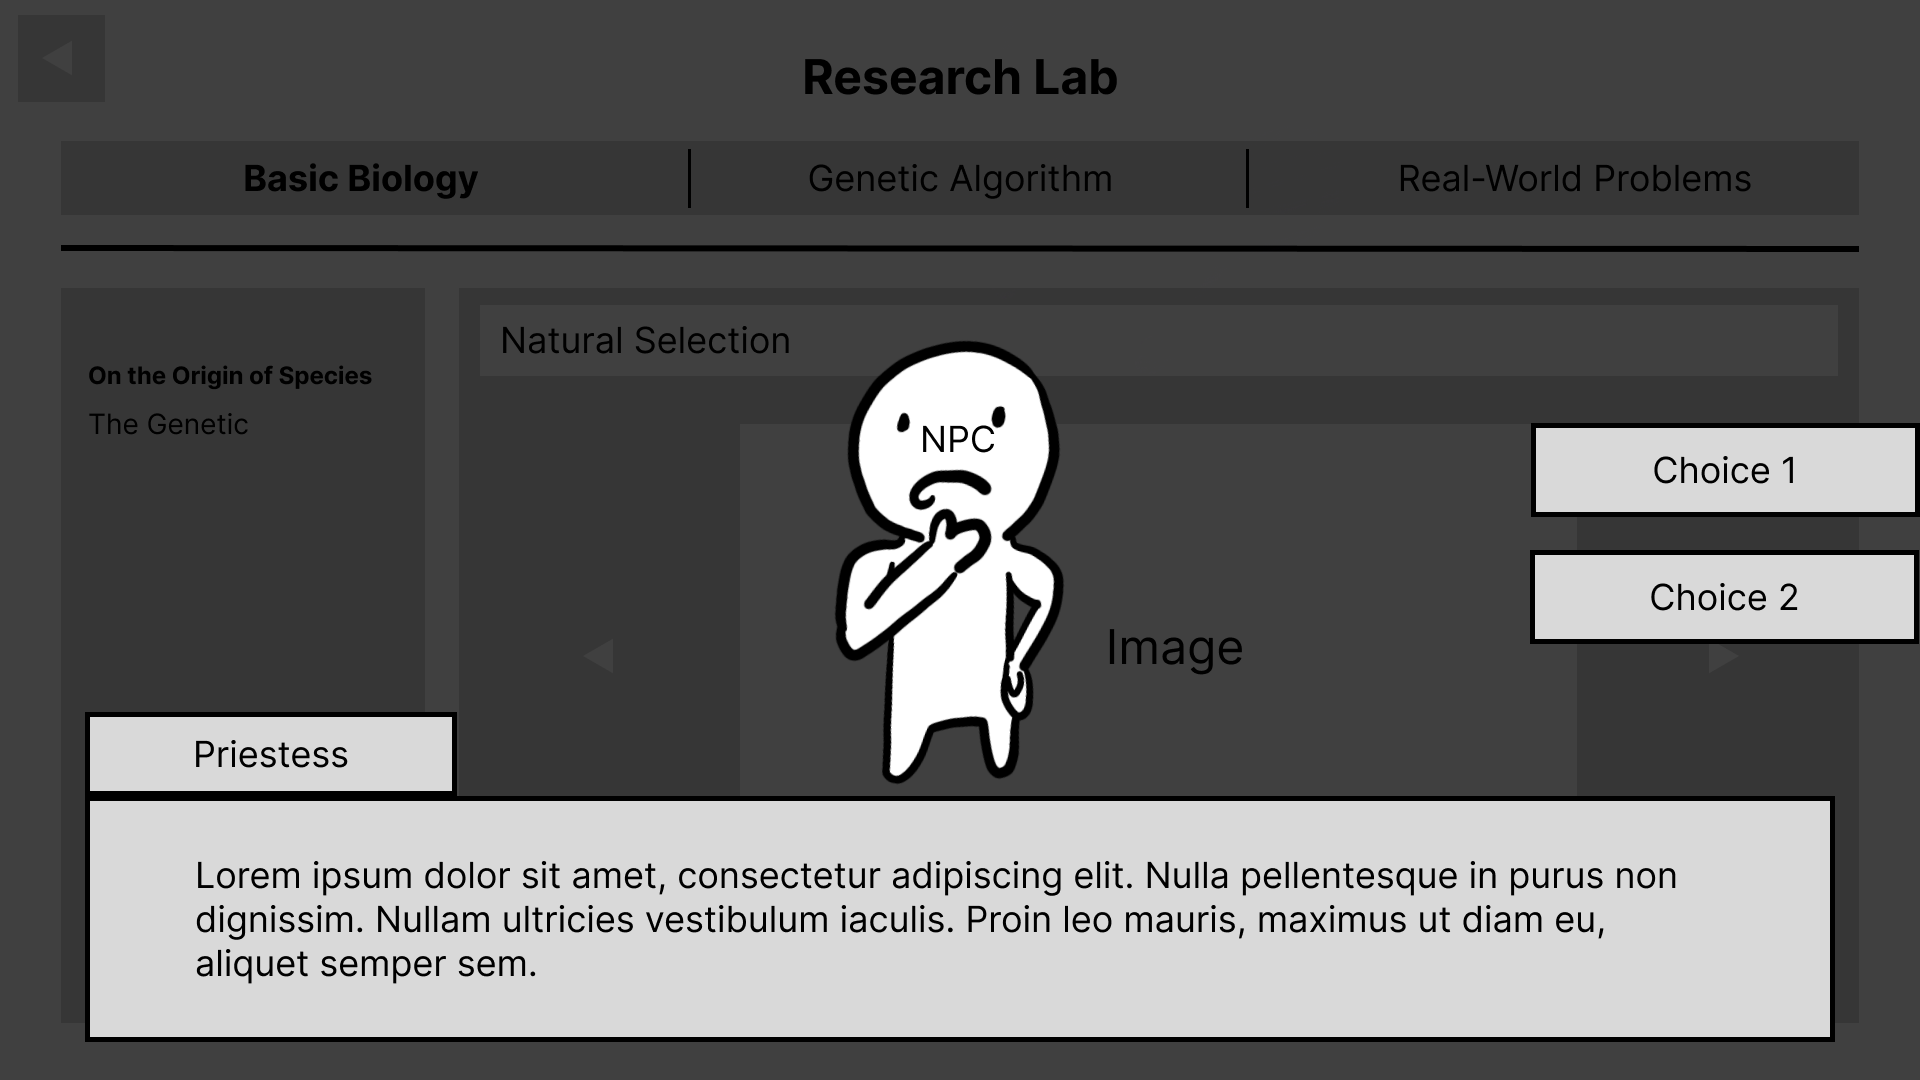
\includegraphics[width=9cm]{figure/design-puzzle-question.png}}
	\captionof{figure}{The Example of Question Scene}
	\label{fig:design-puzzle-question}
	\end{minipage}
	In Figure~\ref{fig:design-puzzle-question}, the players will have to choose the answer from the question. This type of test is for testing the players on how they explain, classify, or identify the lessons they have learned.

	\item Demonstration Puzzle  \\
	\begin{minipage}[c]{\textwidth}\centering
	\fbox{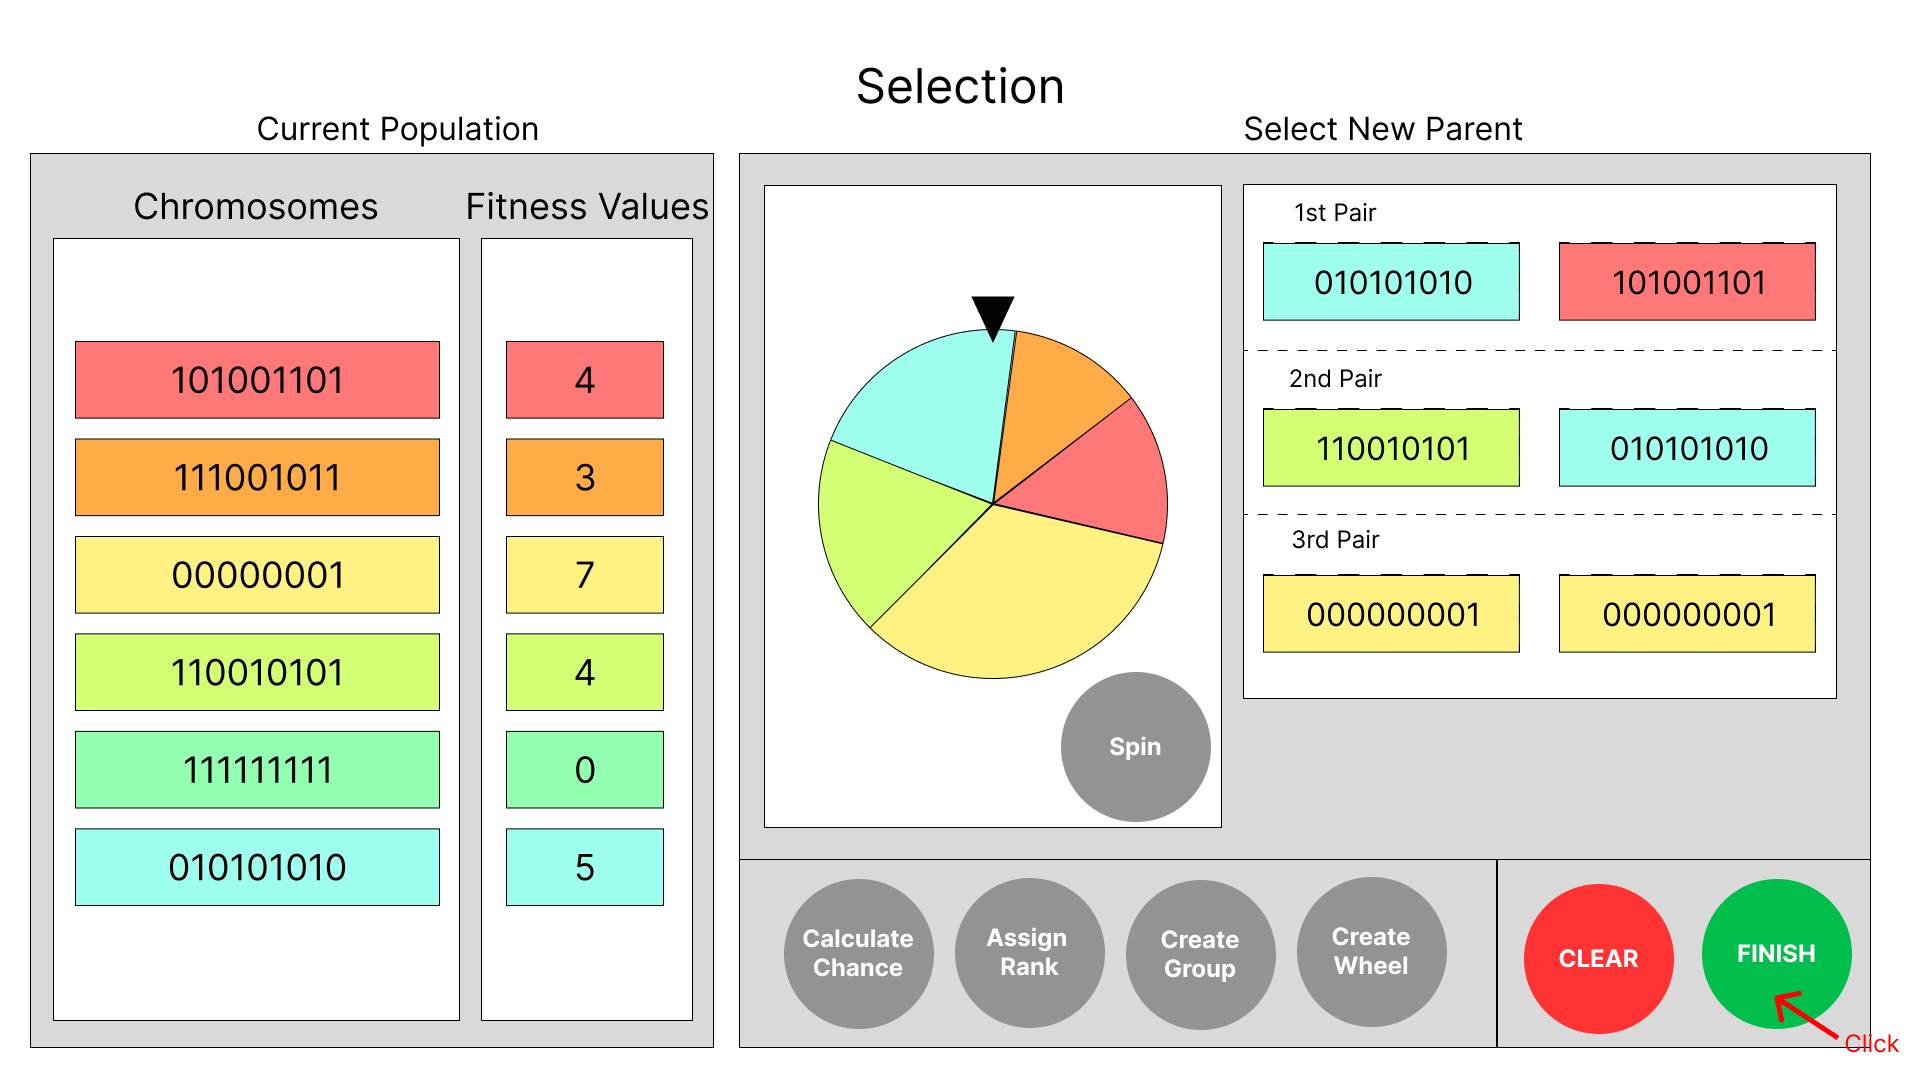
\includegraphics[width=9cm]{figure/design-puzzle-demonstration.png}}
	\captionof{figure}{The Example of Demonstration Puzzle}
	\label{fig:design-puzzle-demonstration}
	\end{minipage}
	This type of puzzle is an open space where the player can operate the objects on the screen to show off their skill. The result of the puzzle will be used as evidence to evaluate the players’ learning level for such criteria. The example of a knapsack decoding demonstration puzzle is shown in Figure~\ref{fig:design-puzzle-demonstration}, the player is required to drag and drop the item into the knapsack above to make the phenotype match the given genotype below.

	\item Problem Solving \\
	\begin{minipage}[c]{\textwidth}\centering
	\fbox{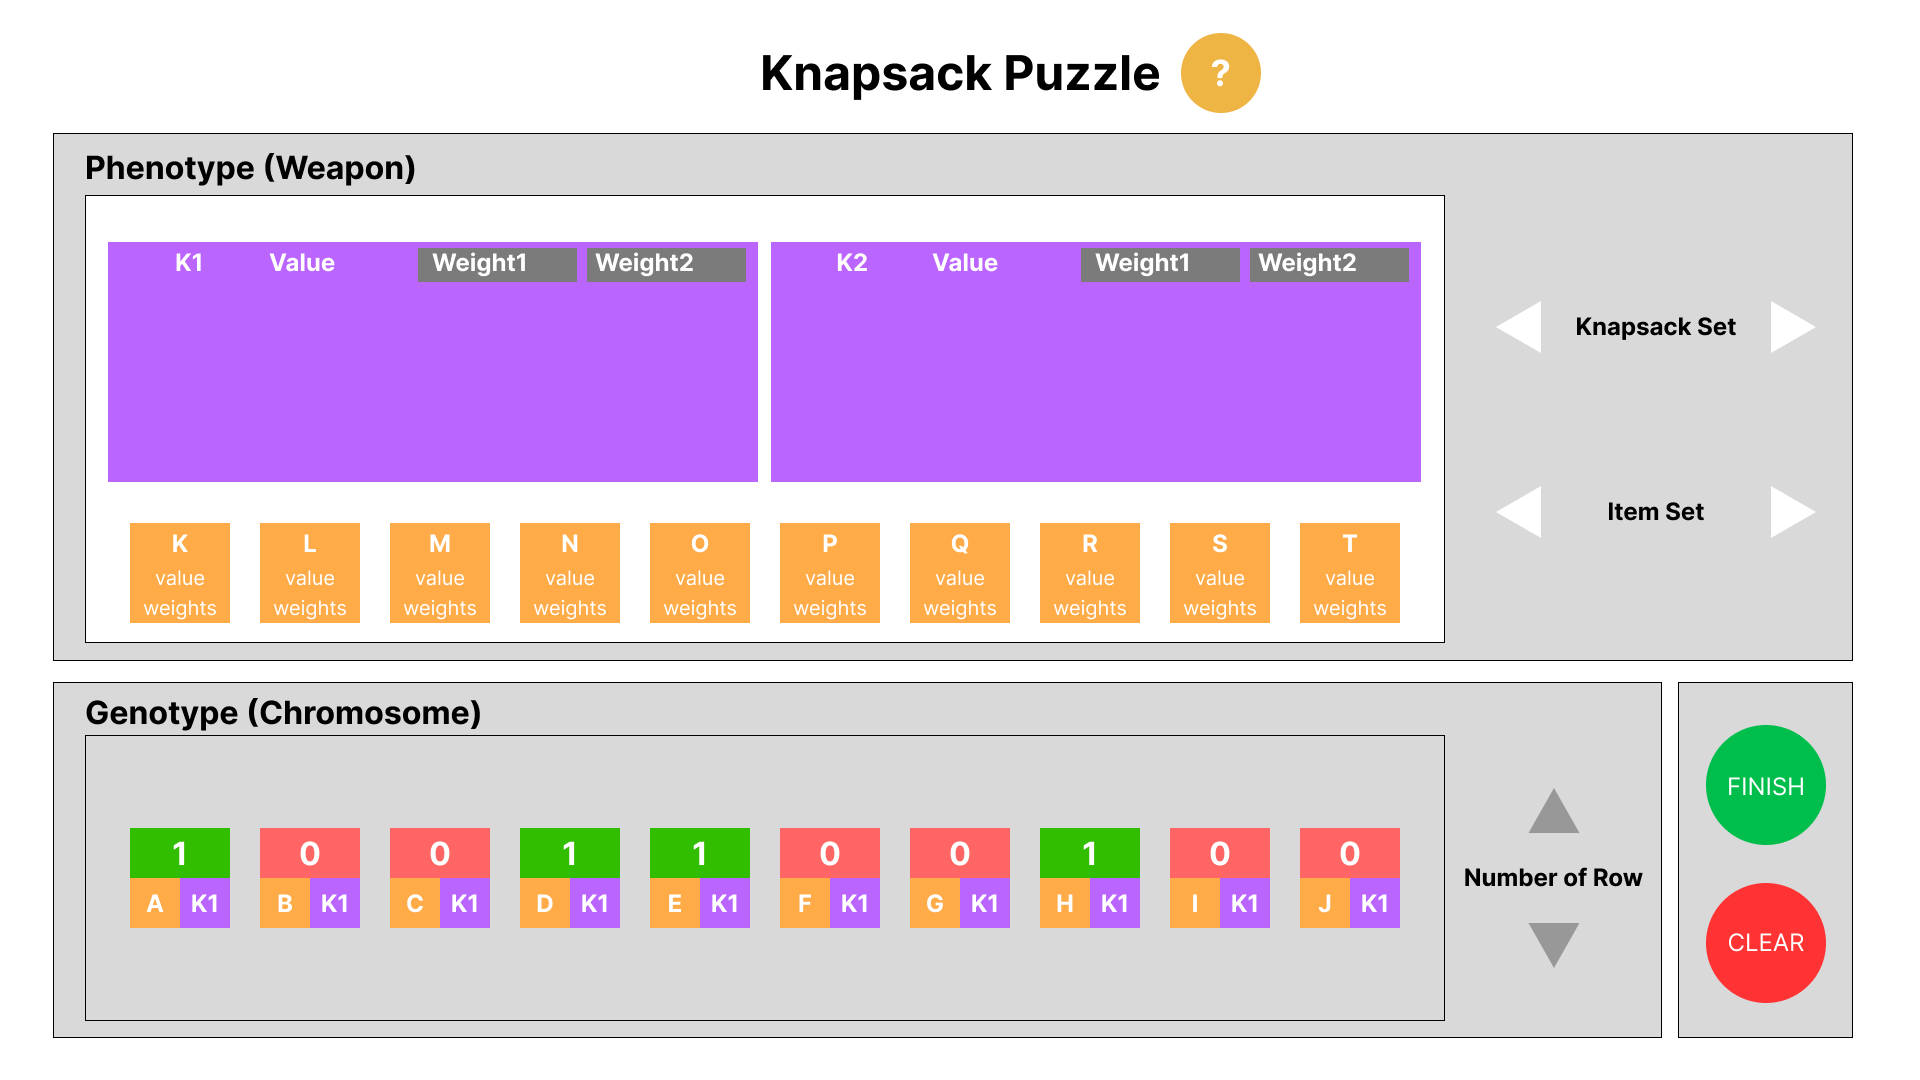
\includegraphics[width=9cm]{figure/design-puzzle-problem-solving.png}}
	\captionof{figure}{The Example of Problem Solving Puzzle}
	\label{fig:design-puzzle-problem-solving}
	\end{minipage}
	To solve the problem, the learner must choose the method of how they can solve the problem and then perform that method to solve it \cite{eberly2022why}. This type of puzzle is very similar to the demonstration puzzle with the extra step of choosing the method. The example of a knapsack solving puzzle is shown in Figure~\ref{fig:design-puzzle-problem-solving}, the extra step of choosing the method is represented as a knapsack and items set selection. The player must click on the button on the right-hand side to choose the correct knapsack and item set. Then perform the drag and drop procedure just like what they must do in the demonstration puzzle to this problem-solving puzzle.
\end{enumerate}

The learning and assessment activity that involves the demonstration and problem-solving level of learning includes the knapsack problem formulation, the parent selection, and the crossover. The detail of the action the player should perform in these puzzles to pass the assessment is described in Table~\ref{tbl:activity-to-achieve-puzzle} below.

% Please add the following required packages to your document preamble:
% \usepackage{longtable}
% Note: It may be necessary to compile the document several times to get a multi-page table to line up properly
\begin{longtable}{|l|l|l|}
\caption{Activity to Achieve the Learning Level of each Criteria}
\label{tbl:activity-to-achieve-puzzle}\\
\hline
\multicolumn{1}{|c|}{\begin{tabular}[c]{@{}c@{}}Rubric Criteria \\ (Topic)\end{tabular}} &
  \multicolumn{1}{c|}{\begin{tabular}[c]{@{}c@{}}Activity to Achieve \\ Demonstration Level\end{tabular}} &
  \multicolumn{1}{c|}{\begin{tabular}[c]{@{}c@{}}Activity to Achieve \\ Problem-solving Level\end{tabular}} \\ \hline
\endhead
%
\begin{tabular}[c]{@{}l@{}}Knapsack \\ Problem \\ Formulation\end{tabular} &
  \begin{tabular}[c]{@{}l@{}}- For problem decoding, drag and \\ drop the item(s) into the knapsack(s)\\ to make the phenotype match the \\ given genotype.\\ - For problem encoding, point and \\ click the bitstring to make the \\ genotype matches the given \\ phenotype.\end{tabular} &
  \begin{tabular}[c]{@{}l@{}}- For problem decoding, choose \\ the correct item(s) and knapsack(s) set. \\ Then perform the action like\\ the demonstration level.\\ - For problem encoding, choose \\ the correct bitstring format. \\ Then perform the action like \\ the demonstration level.\end{tabular} \\ \hline
Parent Selection &
  \begin{tabular}[c]{@{}l@{}}For the given parent selection method \\ and operation buttons, point and click \\ the operation buttons in the correct \\ order until the number of selected \\ parent meet the number of the current \\ population.\end{tabular} &
  \begin{tabular}[c]{@{}l@{}}Give the player the description rather \\ than the exact name of the parent \\ selection method with all operation \\ buttons (unnecessary operation buttons \\ included). The player must choose what \\ selection method the description means \\ and perform the action using only \\ the necessary operation.\end{tabular} \\ \hline
Crossover &
  \begin{tabular}[c]{@{}l@{}}For the given crossover type and \\ the set of chromosomes, the player \\ must pick any pair of chromosomes \\ with the same bitstring format. \\ Then create a random crossover \\ point(s) to suit said crossover type, \\ and drag and drop the proper section \\ of chromosome to complete \\ the crossover.\end{tabular} &
  \begin{tabular}[c]{@{}l@{}}For the given set of parent chromosomes \\ and the wanted child chromosome, \\ the player must pick the proper pair of \\ parents. Then select the necessary \\ crossover point(s), and drag and drop \\ the proper section of the chromosome \\ to make them match the wanted child \\ chromosome.\end{tabular} \\ \hline
\end{longtable}

From the described in-game assessment activities we will use in the game, the assessment result will be kept in the Hall of Intelligence using various types of qualification pieces. Such pieces include copper, silver, and gold. The assessment of activity for the criteria in the rubric Table~\ref{tbl:rubric} is outlined in Table~\ref{tbl:assessment-of-activity} below. The learning performance involving explaining, classifying, and identifying is highlighted and represented in-game using a copper piece. The demonstration level is highlighted and represented in-game using a silver piece. And the gold piece is used for the solving level.

% Please add the following required packages to your document preamble:
% \usepackage{multirow}
% \usepackage[table,xcdraw]{xcolor}
% If you use beamer only pass "xcolor=table" option, i.e. \documentclass[xcolor=table]{beamer}
% \usepackage{longtable}
% Note: It may be necessary to compile the document several times to get a multi-page table to line up properly
\begin{longtable}{|l|lllll|}
\caption{Assessment of the Activity for Criteria}
\label{tbl:assessment-of-activity}\\
\hline
\multicolumn{1}{|c|}{} &
  \multicolumn{5}{c|}{Performance descriptors} \\ \cline{2-6} 
\multicolumn{1}{|c|}{\multirow{-2}{*}{Criteria}} &
  \multicolumn{1}{c|}{Level 1} &
  \multicolumn{1}{c|}{Level 2} &
  \multicolumn{1}{c|}{Level 3} &
  \multicolumn{1}{c|}{Level 4} &
  \multicolumn{1}{c|}{Level 5} \\ \hline
\endhead
%
\begin{tabular}[c]{@{}l@{}}The learner is\\ able to encode\\ the knapsack\\ problem as the \\ chromosome\\ and is able to\\ decode it.\end{tabular} &
  \multicolumn{1}{l|}{\cellcolor[HTML]{FFECD1}\begin{tabular}[c]{@{}l@{}}*Able to \\ explain the \\ problem, \\ constraint, \\ and goal of\\ the Standard, \\ Multidimensi-\\ onal and \\ Multiple \\ Knapsack \\ Problem.\end{tabular}} &
  \multicolumn{1}{l|}{\cellcolor[HTML]{F1F1F1}\begin{tabular}[c]{@{}l@{}}**Able to\\ demonstrate\\ the\\ chromosome\\ encoding and\\ decoding of the\\ Standard and\\ Multidimensio-\\ nal Knapsack \\ Problem.\end{tabular}} &
  \multicolumn{1}{l|}{\cellcolor[HTML]{F1F1F1}\begin{tabular}[c]{@{}l@{}}Able to \\ demonstrate\\ the chromosome\\ encoding and\\ decoding of a\\ Multiple \\ Knapsack \\ Problem.\end{tabular}} &
  \multicolumn{1}{l|}{\cellcolor[HTML]{FFFFE6}\begin{tabular}[c]{@{}l@{}}***Able to \\ solve the \\ chromosome\\ encoding and\\ decoding of\\ the Standard\\ and\\ Multidimen-\\ sional\\ Knapsack\\ Problem.\end{tabular}} &
  \cellcolor[HTML]{FFFFE6}\begin{tabular}[c]{@{}l@{}}Able to solve\\ the \\ chromosome\\ encoding and\\ decoding of a\\ Multiple\\ Knapsack\\ Problem.\end{tabular} \\ \hline
\begin{tabular}[c]{@{}l@{}}The learner is\\ able to solve\\ the parent\\ chromosome\\ selection\\ problem in\\ the Genetic\\ Algorithms.\end{tabular} &
  \multicolumn{1}{l|}{\cellcolor[HTML]{FFECD1}\begin{tabular}[c]{@{}l@{}}Able to\\ explain the\\ meaning and\\ purpose of a\\ parent\\ chromosome\\ selection in a\\ Genetic\\ Algorithm.\end{tabular}} &
  \multicolumn{1}{l|}{\cellcolor[HTML]{F1F1F1}\begin{tabular}[c]{@{}l@{}}Able to\\ demonstrate\\ the process of\\ the \\ Tournament-\\ based\\ Selection.\end{tabular}} &
  \multicolumn{1}{l|}{\cellcolor[HTML]{F1F1F1}\begin{tabular}[c]{@{}l@{}}Able to \\ demonstrate \\ the process of\\ the Roulette\\ Wheel\\ Selection and\\ Rank-based \\ Selection.\end{tabular}} &
  \multicolumn{1}{l|}{\cellcolor[HTML]{FFFFE6}\begin{tabular}[c]{@{}l@{}}Able to solve\\ parent\\ selection \\ problems \\ using \\ Tournament-\\ based \\ Selection.\end{tabular}} &
  \cellcolor[HTML]{FFFFE6}\begin{tabular}[c]{@{}l@{}}Able to solve\\ parent \\ selection \\ problems \\ using Roulette\\ Wheel\\ Selection and\\ Rank-based\\ Selection.\end{tabular} \\ \hline
\begin{tabular}[c]{@{}l@{}}The learner is\\ able to solve\\ the \\ chromosome\\ crossover\\ problem in\\ the Genetic\\ Algorithms.\end{tabular} &
  \multicolumn{1}{l|}{\cellcolor[HTML]{FFECD1}\begin{tabular}[c]{@{}l@{}}Able to\\ explain the\\ meaning and\\ purpose of a\\ chromosome\\ crossover in\\ a Genetic\\ Algorithm.\end{tabular}} &
  \multicolumn{1}{l|}{\cellcolor[HTML]{FFECD1}\begin{tabular}[c]{@{}l@{}}Able to classify\\ between\\ Single-point\\ Crossover, \\ Two-point \\ Crossover, and\\ Uniform \\ Crossover.\end{tabular}} &
  \multicolumn{1}{l|}{\cellcolor[HTML]{F1F1F1}\begin{tabular}[c]{@{}l@{}}Able to\\ demonstrate\\ the process of\\ the Single-point\\ Crossover and\\ Two-point \\ Crossover.\end{tabular}} &
  \multicolumn{1}{l|}{\cellcolor[HTML]{FFFFE6}\begin{tabular}[c]{@{}l@{}}Able to solve\\ the \\ chromosome\\ crossover\\ problem using\\ the\\ Single-point\\ Crossover \\ and Two-point \\ Crossover.\end{tabular}} &
   \\ \hline
\begin{tabular}[c]{@{}l@{}}The learner is\\ able to \\ identify the \\ basic  method \\ of \\ improvement\\ technique in\\ the Genetic\\ Algorithm\\ including\\ elitism and\\ mutation.\end{tabular} &
  \multicolumn{1}{l|}{\cellcolor[HTML]{FFECD1}\begin{tabular}[c]{@{}l@{}}Able to\\ explain the\\ meaning and\\ purpose of\\ Elitism and \\ mutation in \\ Genetic \\ Algorithm.\end{tabular}} &
  \multicolumn{1}{l|}{\cellcolor[HTML]{FFECD1}\begin{tabular}[c]{@{}l@{}}Able to classify\\ between \\ Elitism, Bit Flip\\ Mutation, \\ Flip-Bit \\ Mutation, and \\ Boundary \\ Mutation.\end{tabular}} &
  \multicolumn{1}{l|}{\cellcolor[HTML]{FFECD1}\begin{tabular}[c]{@{}l@{}}Able to identify\\ the type of\\ improvement \\ techniques \\ including \\ Elitism, Bit Flip\\ Mutation, Flip \\ Bit Mutation, \\ and Boundary \\ Mutation.\end{tabular}} &
  \multicolumn{1}{l|}{} &
   \\ \hline
\end{longtable}
Note: *Orange highlighted = Copper Jigsaw piece, **Gray highlighted  = Silver Jigsaw piece, ***Yellow highlighted = Gold Jigsaw Piece
%\item Puzzle/Test Structure \\
%	The game will use puzzles and tests to evaluate the players about the knowledge and understanding of the lessons as in the assessment Table~\ref{tbl:rubric} and use it as exercises to help players apply their knowledge after learning them.
%	\begin{itemize}
%		
%		\item Puzzle/Test Appearance \\
%		The players will encounter puzzle in 2 different situations as following:
%		\begin{enumerate}
%			\item After the players finish learning the lesson from the research lab, The players will have a button to solve the puzzle to complete the lesson.
%			\item When the farms or factories break down, the players will have to solve the puzzle to fix and continue to use it.
%		\end{enumerate}
%		
%		\item Type of Puzzle/Test \\
%		The puzzle/test that the players will encounter will have 3 types of puzzle/test as following: 
%		\begin{enumerate}
%			\item Questions Test \\
%			\begin{minipage}[c]{\textwidth}\centering
%			\fbox{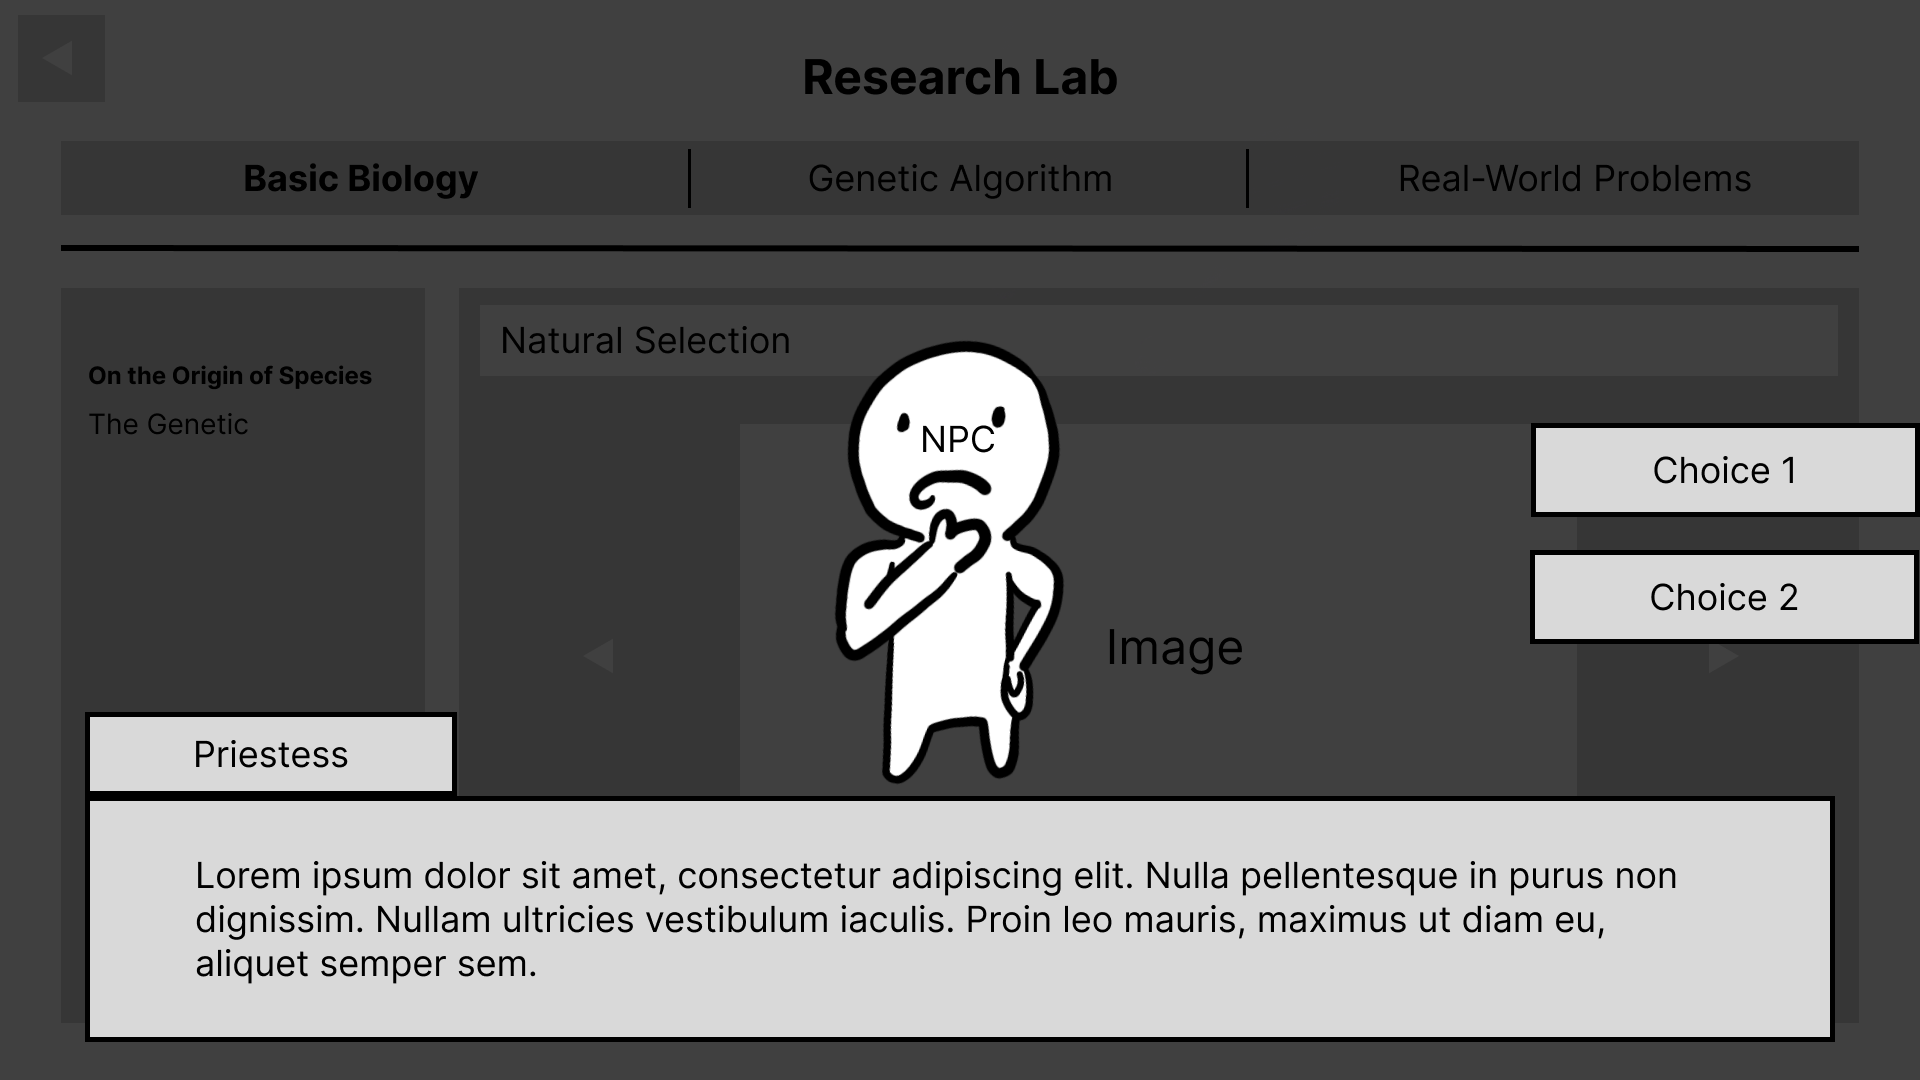
\includegraphics[width=9cm]{figure/design-puzzle-question.png}}
%			\captionof{figure}{The Example of Questions Test Scene}
%			\label{fig:design-puzzle-question}
%			\end{minipage}
%			In Figure~\ref{fig:design-puzzle-question}, the players will have to choose the answer from the question. This type of test is for  testing the players about how they explain, classify, or identify the lessons they have learned.
%
%			\item Demonstration \\
%			\begin{minipage}[c]{\textwidth}\centering
%			\fbox{\includegraphics[width=9cm]{figure/design-puzzle-demonstration.png}}
%			\captionof{figure}{The Example of Demonstration Puzzle}
%			\label{fig:design-puzzle-demonstration}
%			\end{minipage}
%			In Figure~\ref{fig:design-puzzle-demonstration}, the puzzle/test is an open space where the learner is free to choose what process to perform and free to decide when to perform it. The puzzle will record the process the players perform to evaluate the players’ understanding.
%
%			\item Problem Solving \\
%			\begin{minipage}[c]{\textwidth}\centering
%			\fbox{\includegraphics[width=9cm]{figure/design-puzzle-problem-solving.png}}
%			\captionof{figure}{The Example of Problem Solving Puzzle}
%			\label{fig:design-puzzle-problem-solving}
%			\end{minipage}
%			In Figure~\ref{fig:design-puzzle-problem-solving}, the players will have to perform the action to solve the problem from the question or situation. The player is free to decide what method they will use and how the procedures perform. Designing this way, the puzzle would be able to assess the true learning level of the player \cite{eberly2022why}.
%		\end{enumerate}
%	\end{itemize}
%\end{enumerate}

%Explain the design (how you plan to implement your work) of your project. Adjust the section titles below to suit the types of your work. Detailed physical design like circuits and source codes should be placed in the appendix.
%
%\section{System Architecture}
%
%\begin{table}[!h]
%\centering
%\caption{test table x1}\label{tbl:symbols}
%\begin{tabular}{@{}p{0.07\textwidth}|p{0.7\textwidth}p{0.1\textwidth}}\hline
%\multicolumn{2}{l}{\textbf{SYMBOL}}  & \textbf{UNIT} \\ \hline 
%$\alpha$ & Test variable\hfill & m$^2$ \\
%$\lambda$ & Interarrival rate\hfill &  jobs/second\\
%$\mu$ & Service rate\hfill & jobs/second \\ \hline
%\end{tabular}
%%\begin{tabular}{c|c} \hline
%% $\alpha$ & $\beta$ \\ \hline
%% $\delta$ & $\mu$ \\ \hline
%%\end{tabular}
%\end{table}
%
%\section{System Specifications and Requirements}
%
%\section{Hardware Module 1}
%\subsection{Component 1}
%\subsection{Logical Circuit Diagram}
%
%\section{Hardware Module 2}
%\subsection{Component 1}
%\subsection{Component 2}
%
%\section{Path Finding Algorithm}
%
%\section{Database Design}
%
%\section{GUI Design}

%%%%%%%%%%%%%%%%%%%%%%%%%%%%%%%%%%%%%%%%%%%%%%%%%%%%%%%%%%%%%%%%%%
\subsection{Prototyping and Usability Testing}
For typical education design using the ADDIE model, the developed contents may be used in the education simulation to test the feasibility of the project. As an educational game, we decide to conduct usability testing instead since it's more suitable for the game and we can't directly perform the learning simulation. \\
Since we haven't developed the actual working software yet in this phase, we choose to develop the simple wireframe prototype, a series of mock-up screens simulating the working software, for testing purposes. Then we record the prototype as a video together with the narration of how things work. \\
After the prototyping is done, we decide to conduct the test on a small group of the target user which is the student that currently studies in the field of computer engineering. The data we want from this test is mainly opinions about our current design. So, we sent the video of the prototype to the tester and request them to answer the post-test question about their opinion on the design. The six questions in total with the possible answer will be shown in Table~\ref{tbl:usability-test-questionaire}.

% Please add the following required packages to your document preamble:
% \usepackage{longtable}
% Note: It may be necessary to compile the document several times to get a multi-page table to line up properly
\begin{longtable}{|l|l|}
\caption{The Questionnaire for Usability Testing}
\label{tbl:usability-test-questionaire}\\
\hline
\multicolumn{1}{|c|}{Question}                                                                                   & \multicolumn{1}{c|}{Possible Answer}          \\ \hline
\endhead
%
Have you ever studied Genetic Algorithms?                                                                        & Yes/No                                        \\ \hline
What do you think about this design?                                                                             & Score from 1 (Terrible) to 5 (Excellent)      \\ \hline
What do you think about the user interface?                                                                      & Score from 1 (Hard to Use) to 5 (Easy to Use) \\ \hline
\begin{tabular}[c]{@{}l@{}}What do you think about the complexity of \\ the gameplay?\end{tabular} &
  \begin{tabular}[c]{@{}l@{}}Score from 1 (Too Complicated) to 5 \\ (Too Simple)\end{tabular} \\ \hline
\begin{tabular}[c]{@{}l@{}}If you notice any issue that makes this game \\ terrible, what is it?\end{tabular}    & Short text                                    \\ \hline
\begin{tabular}[c]{@{}l@{}}If you could change one thing in this game, \\ what would it be and why?\end{tabular} & Short text                                    \\ \hline
\end{longtable}



%%%%%%%%%%%%%%%%%%%%%%%%%%%%%%%%%%%%%%%%%%%%%%%%%%%%%%%%%%%%%%
%%%%%%%%%%%%%%%%%%%% Experiments %%%%%%%%%%%%%%%%%%%%%%%%%%%%%
%%%%%%%%%%%%%%%%%%%%%%%%%%%%%%%%%%%%%%%%%%%%%%%%%%%%%%%%%%%%%%%
%\chapter{Implementation Results}
\chapter{Implementation Results}
In this chapter, according to the ADDIE model, we will introduce our work in the implementation phase and evaluation phase of our project. This includes the result of usability testing, the software implementation result, and the user satisfaction evaluation result.


%%%%%%%%%%%%%%%%%%%%%%%%%%%%%%%%%%%%%%%%%%%%%%%%%%%%%%%%%%%%%%%%%%
%%%%%%%%%%%%%%%%%%%%%%%%%%%%%%%%%%%%%%%%%%%%%%%%%%%%%%%%%%%%%%%%%%
\section{Usability Testing Result}
We conduct usability testing using the information we already mentioned in the development phase in chapter 3. The test takes place in the first week of February 2023, which is in the first sprint of semester 2. The summary of the responses from 13 testers will be described.

% Please add the following required packages to your document preamble:
% \usepackage{longtable}
% Note: It may be necessary to compile the document several times to get a multi-page table to line up properly
\begin{longtable}{|l|l|}
\caption{The Summary Response to Usability Questionnaire}
\label{tbl:usability-test-summary-response}\\
\hline
\multicolumn{1}{|c|}{Question} &
  \multicolumn{1}{c|}{Response} \\ \hline
\endhead
%
Have you ever studied Genetic Algorithms? &
  8 Yes, 5 No \\ \hline
What do you think about this design? &
  \begin{tabular}[c]{@{}l@{}}An average score is equal to 4.0\\ (Close to excellent)\end{tabular} \\ \hline
What do you think about the user interface? &
  \begin{tabular}[c]{@{}l@{}}An average score is equal to 4.2 \\ (Close to easy to use)\end{tabular} \\ \hline
\begin{tabular}[c]{@{}l@{}}What do you think about the complexity of \\ the gameplay?\end{tabular} &
  \begin{tabular}[c]{@{}l@{}}An average score is equal to 2.2 \\ (Close to too complicated)\end{tabular} \\ \hline
\begin{tabular}[c]{@{}l@{}}If you notice any issue that makes this game \\ terrible, what is it?\end{tabular} &
  Optional short text answer \\ \hline
\begin{tabular}[c]{@{}l@{}}If you could change one thing in this game, \\ what would it be and why?\end{tabular} &
  Optional short text answer \\ \hline
\end{longtable}

From the responses in Table~\ref{tbl:usability-test-summary-response} above, the overall design and the user interface have no serious problems. For the complexity of the game, the tester's overall opinion indicates that they think the gameplay is a bit too complicated. However, we think such an opinion is acceptable because our game is an educational game with puzzle gameplay which may require a portion of learning before clearly understanding the puzzle. The other 2 question is optional short-answer questions which turn out that there is some improvement suggestion and question about some specific game mechanic but still have no severe problems. So, we continue the implementation with no major change in the design. Please note that the full version of the response can be reviewed in Appendix. %~\ref{appendix:usability-test-responses}.


%%%%%%%%%%%%%%%%%%%%%%%%%%%%%%%%%%%%%%%%%%%%%%%%%%%%%%%%%%%%%%%%%%
%%%%%%%%%%%%%%%%%%%%%%%%%%%%%%%%%%%%%%%%%%%%%%%%%%%%%%%%%%%%%%%%%%
\section{Implementation Result}
After finishing all nine sprints, we can deploy a playable prototype on Windows. However, there are still known and unknown bugs that we are still searching for and fixing. We collect feedback on the game by both testing the game ourselves and inviting people from the target group to play. \\
The following section will feature game interfaces and their functionalities.
\begin{enumerate}
	\item Title \\
	\begin{minipage}[c]{\textwidth}\centering
	\includegraphics[width=14cm]{figure/screenshot/screenshot-title.png}
	\captionof{figure}{Title Screenshot}
%	\label{fig:screenshot-title}
	\end{minipage}
	This scene will display every time players enter the game. Its main features include starting new game, continue from old save (if possible), adjust volume in settings, and exit game.

	\item Hub \\
	\begin{minipage}[c]{\textwidth}\centering
	\includegraphics[width=14cm]{figure/screenshot/screenshot-hub-main.png}
	\captionof{figure}{Main Hub Screenshot (Overview)}
	\end{minipage}
	\begin{minipage}[c]{\textwidth}\centering
	\includegraphics[width=14cm]{figure/screenshot/screenshot-hub-fix.png}
	\captionof{figure}{Main Hub Screenshot (Fixing facilities)}
	\end{minipage}
	\begin{minipage}[c]{\textwidth}\centering
	\includegraphics[width=14cm]{figure/screenshot/screenshot-hub-quest.png}
	\captionof{figure}{Main Hub Screenshot (Quest Overlay)}
	\end{minipage}
	This scene serves as a general hub for players to navigate through most parts of the game. In the middle, there are factory (upper row) and farm (lower row) buttons. Apart from taking players to the farm and factory scene, they also indicate the lock/unlock status of the facility and its condition, which players can click on it to fix that facility. The quest tab on the left will display the current main quest and accepted side quests. The habitat, the city, and the research lab will take players to their respective scenes. The calendar tab on the top middle will take players to the calendar scene while displaying the current date in the game. The upper left tab shows the current amount of money players possess. \\
	Apart from navigation, there are also chances for a random capybara to spawn, which players could click to pet them, and they might give some rewards. 

	\item Farm \\
	\begin{minipage}[c]{\textwidth}\centering
	\includegraphics[width=14cm]{figure/screenshot/screenshot-farm.png}
	\captionof{figure}{Farm Screenshot}
	\end{minipage}
	Players can breed mechs on the farm to improve their quality or make them fit with their preferences within this scene. On the left side is a space for mechs to walk around, and the panel below displays the status of the farm if it is currently idle, breeding, or broken. The main functionalities of this scene are on the right side, which consists of three panels. The first panel lets players edit the fitness function of this farm so they can prioritize what mechs they want. The second one is for breeding configuration. Players can choose means of parent selection, crossing over, and other relevant variables as they want. The last panel displays the list of the current population on this farm. Players can click to view more details about the mech.

	\item Factory \\
	\begin{minipage}[c]{\textwidth}\centering
	\includegraphics[width=14cm]{figure/screenshot/screenshot-factory.png}
	\captionof{figure}{Factory Screenshot}
	\end{minipage}
	Similar to farms, factories let players manage their weapons. It has a similar layout to the farm, with chromosome visualizations on the left, control panels on the right, and a status panel at the bottom. The only difference is that the first panel is a weapon description instead of fitness adjustments, as the fitness function of the weapon is controlled by the factory.

	\item Habitat \\
	\begin{minipage}[c]{\textwidth}\centering
	\includegraphics[width=14cm]{figure/screenshot/screenshot-habitat.png}
	\captionof{figure}{Habitat Screenshot}
	\end{minipage}
	The mechs can be assigned to other facilities (if available) within this scene. The order of the mechs in each farm is set by separated fitness priority, which can be edited by players.

	\item Research Lab \\
	\begin{minipage}[c]{\textwidth}\centering
	\includegraphics[width=14cm]{figure/screenshot/screenshot-researchLab.png}
	\captionof{figure}{Research Lab Screenshot}
	\end{minipage}
	Players can unlock and review learned lessons in this scene. After unlocking a new lesson, a cutscene will play. Furthermore, the Upper left buttons will navigate players to the Hall of Capybara and Hall of Intelligence respectively.

	\item Cutscene \\
	\begin{minipage}[c]{\textwidth}\centering
	\includegraphics[width=14cm]{figure/screenshot/screenshot-cutscene-dialogue.png}
	\captionof{figure}{Cutscene Screenshot (Dialogue)}
	\end{minipage}
	\begin{minipage}[c]{\textwidth}\centering
	\includegraphics[width=14cm]{figure/screenshot/screenshot-cutscene-choice.png}
	\captionof{figure}{Cutscene Screenshot (Choice)}
	\end{minipage}
	Cutscenes can display stories, lessons, and exams in a Visual Novel style. Players can inspect previous dialogues with the Log button, make the next dialogue display automatically with the Auto button, and skip the whole conversation with the Skip button if it is skippable.

	\item Hall of Intelligence \\
	\begin{minipage}[c]{\textwidth}\centering
	\includegraphics[width=14cm]{figure/screenshot/screenshot-HoI.png}
	\captionof{figure}{Hall of Intelligence Screenshot}
	\end{minipage}
	This scene shows sets of jigsaw pieces representing categories of achievements players received in the game. When clicking on it, players can take a test to increase their rank. It also shows players’ names, the number of passed days, the current main quest, and the number of times players have succeeded or failed each level of puzzles.

	\item Puzzles \\
	\begin{minipage}[c]{\textwidth}\centering
	\includegraphics[width=14cm]{figure/screenshot/screenshot-puzzle-selection.png}
	\captionof{figure}{ Puzzle Screenshot (Selection)}
	\end{minipage}
	\begin{minipage}[c]{\textwidth}\centering
	\includegraphics[width=14cm]{figure/screenshot/screenshot-puzzle-crossover.png}
	\captionof{figure}{Puzzle Screenshot (Crossover)}
	\end{minipage}
	\begin{minipage}[c]{\textwidth}\centering
	\includegraphics[width=14cm]{figure/screenshot/screenshot-puzzle-knapsack.png}
	\captionof{figure}{Puzzle Screenshot (Knapsack)}
	\end{minipage}
	Players will solve a puzzle when taking tests to increase a jigsaw rank or fix a facility. There are multiple types of puzzles depending on types of knowledge; knapsack puzzles and genetic algorithm-related puzzles, and level of assessment, such as question, demonstration, and solving. The full gameplay of all the puzzle material can be found in Appendix.


	\item Hall of Capybara \\
	\begin{minipage}[c]{\textwidth}\centering
	\includegraphics[width=14cm]{figure/screenshot/screenshot-HoC.png}
	\captionof{figure}{Hall of Capybara Screenshot}
	\end{minipage}
	This scene shows which capybara players have seen and how often they have greeted them.

	\item Calendar \\
	\begin{minipage}[c]{\textwidth}\centering
	\includegraphics[width=14cm]{figure/screenshot/screenshot-calendar.png}
	\captionof{figure}{Calendar Screenshot}
	\end{minipage}
	The calendar shows the current date, or the selected date events such as side quest submission deadline. Players can either end their day or skip to the selected date.
	
	\item City \\
	\begin{minipage}[c]{\textwidth}\centering
	\includegraphics[width=14cm]{figure/screenshot/screenshot-city.png}
	\captionof{figure}{City Screenshot}
	\end{minipage}
	This scene serves as a secondary hub. It takes players to other scenes: the quest, the arena, the shop, and the main hub.

	\item Questboard \\
	\begin{minipage}[c]{\textwidth}\centering
	\includegraphics[width=14cm]{figure/screenshot/screenshot-quest-overview.png}
	\captionof{figure}{Questboard Screenshot (Overview)}
	\end{minipage}
	\begin{minipage}[c]{\textwidth}\centering
	\includegraphics[width=14cm]{figure/screenshot/screenshot-quest-detail.png}
	\captionof{figure}{Questboard Screenshot (Detail)}
	\end{minipage}
	This page helps players manage their side quests. They can accept available quests on the left side, and they will appear on the right side to be submitted. When players submit a quest, they will receive rewards according to the similarity between the requested mech and the submitted mech. If players fail to submit a quest before its deadline, players will have to abandon that quest and pay a penalty.

	\item Shop \\
	\begin{minipage}[c]{\textwidth}\centering
	\includegraphics[width=14cm]{figure/screenshot/screenshot-shop.png}
	\captionof{figure}{Shop Screenshot}
	\end{minipage}
	Players can replenish their mech population by purchasing new mechs in this scene. They can inspect its information by hovering over it. After a mech is bought, it will be out of stock until the shop is restocked.

	\item Arena \\
	\begin{minipage}[c]{\textwidth}\centering
	\includegraphics[width=14cm]{figure/screenshot/screenshot-arena-prep.png}
	\captionof{figure}{Arena Screenshot (Preparation)}
	\end{minipage}
	\begin{minipage}[c]{\textwidth}\centering
	\includegraphics[width=14cm]{figure/screenshot/screenshot-arena-battle.png}
	\captionof{figure}{Arena Screenshot (Battle)}
	\end{minipage}
	The arena consists of two phases, the preparation, and the battle. Players can select which mech and weapon to put in the team by themselves or set it automatically. The battle record of the day and the element multiplier are displayed on the top. After selecting an opponent, the battle sequence will be initiated. In the end, players will receive a reward or penalty depending on the battle result.

\end{enumerate}


% preliminary result in midterm2 report
%After we begin the software implementation for 2 Sprints, all demonstration and problem-solving puzzles that are used as learning and assessment activities are finished along with the great progression of other crucial systems related to such puzzles. The portion of the weapon factory, monster farm, main game page, and saving system is workable but not completely done. Most of the art assets also be created along with said systems. \\
%Figure~\ref{fig:implement-puzzle-knapsack} is the screenshot of the working game scene of the knapsack problem decoding puzzle. The screenshot of the parent selection puzzle is shown in Figure~\ref{fig:implement-puzzle-selection}. And the screenshot of the crossover puzzle also represents in Figure~\ref{fig:implement-puzzle-crossover}.  \\
%
%\begin{minipage}[c]{\textwidth}\centering
%\includegraphics[width=14cm]{figure/implement-puzzle-knapsack.png}
%\captionof{figure}{Screenshot of Knapsack Decoding Puzzle}
%\label{fig:implement-puzzle-knapsack}
%\end{minipage}
%\begin{minipage}[c]{\textwidth}\centering
%\includegraphics[width=14cm]{figure/implement-puzzle-selection.png}
%\captionof{figure}{Screenshot of Tournament-based Selection Puzzle}
%\label{fig:implement-puzzle-selection}
%\end{minipage}
%
%\pagebreak
%\begin{minipage}[c]{\textwidth}\centering
%\includegraphics[width=14cm]{figure/implement-puzzle-crossover.png}
%\captionof{figure}{Screenshot of Single-point Crossover Puzzle}
%\label{fig:implement-puzzle-crossover}
%\end{minipage}
%
%Note that both the demonstration and problem-solving levels of each puzzle type can be assessed using the same puzzle scene with some different settings. And our implemented game scene can set and check the conditions to suit the criteria we already mentioned in the development phase in chapter 3.\\
%These screenshots below (Figure~\ref{fig:implement-mainpage} to Figure~\ref{fig:implement-calendar}) are from the main menu, weapon factory, mech farm, and calendar. As explained in the last chapter, the main menu will be used as a hub to access other parts of the game, such as factories and farms in the middle, city and calendar from the sides. Farms and factories will control their respective populations, from storing to breeding new generations, which players can adjust some parameters as they will. Apart from displaying the date and event within that day, the calendar will let the player end their day or skip to future days, which also results in saving the game in the process.
%
%\begin{minipage}[c]{\textwidth}\centering
%\includegraphics[width=14cm]{figure/implement-mainpage.png}
%\captionof{figure}{Screenshot of Main Menu}
%\label{fig:implement-mainpage}
%\end{minipage}
%\begin{minipage}[c]{\textwidth}\centering
%\includegraphics[width=14cm]{figure/implement-factory.png}
%\captionof{figure}{Screenshot of Weapon Factory}
%\label{fig:implement-factory}
%\end{minipage}
%\begin{minipage}[c]{\textwidth}\centering
%\includegraphics[width=14cm]{figure/implement-farm.png}
%\captionof{figure}{Screenshot of Mech Farm}
%\label{fig:implement-farm}
%\end{minipage}
%\begin{minipage}[c]{\textwidth}\centering
%\includegraphics[width=14cm]{figure/implement-calendar.png}
%\captionof{figure}{Screenshot of Calendar}
%\label{fig:implement-calendar}
%\end{minipage}


%%%%%%%%%%%%%%%%%%%%%%%%%%%%%%%%%%%%%%%%%%%%%%%%%%%%%%%%%%%%%%%%%%
%%%%%%%%%%%%%%%%%%%%%%%%%%%%%%%%%%%%%%%%%%%%%%%%%%%%%%%%%%%%%%%%%%
\section{User Satisfaction Evaluation Result}
We conducted user satisfaction testing with the completed version of the game using a survey form. Determining the satisfaction level of each system in the game from the user's playthrough and the knowledge of the Genetic Algorithm gained. \\
The test took place from May 10th to May 17th, 2023, and the survey was distributed in a Google Form. The form included a link to the itch.io page of the game, where players could choose to play the game in their preferred browser or download it to play locally on their desktop. \\
In the form, testers were required to play the game and achieve at least a silver jigsaw in each of the trays in the Hall of Intelligence. They were asked to upload a screenshot of their Hall of Intelligence, as shown in Figure~\ref{fig:result-example-hoi-screenshot} to provide their progress in the game. \\
The results provided a comprehensive overview of user perceptions and highlighted opportunities for improvement. The summary of these responses from 92 testers will be described in the following sections. \\
\begin{minipage}[c]{\textwidth}\centering
\includegraphics[width=14cm]{figure/result-example-hoi-screenshot.png}
\captionof{figure}{Example of Screenshot of the Hall Of Intelligence from the tester}
\label{fig:result-example-hoi-screenshot}
\end{minipage}
The results of the survey provide a comprehensive overview of user perceptions and highlight opportunities for improvement.The summary of the responses from 30 testers will be described.

\begin{itemize}
	\item Summary Of Tester Data \\
	There were 92 participants who responded to the survey form, all of whom were university students. Out of the participants, 83 were freshmen or first-year students, 8 were seniors or final-year students, and there was one sophomore or second-year student. Among the participants, 88 were studying computer engineering, while 4 participants were studying in each of the following fields: computer and information technology, computer science, media technology game development, Institute of field robotics (FIBO), and business administration.

	\item Overall Satisfaction Result \\
	The overall results of the satisfaction levels for each system in the game are shown in the Table~\ref{tbl:satisfactory-test-summary-response} below.
% Please add the following required packages to your document preamble:
% \usepackage{longtable}
% Note: It may be necessary to compile the document several times to get a multi-page table to line up properly
\begin{longtable}{|l|l|}
\caption{The Summary Response of User Satisfaction Survey to the Overall System of the Game}
\label{tbl:satisfactory-test-summary-response}\\
\hline
Question &
  Response \\ \hline
\endhead
%
\begin{tabular}[c]{@{}l@{}}What your satisfaction level of \\ the learning materials and teaching \\ cutscene in Research Lab?\end{tabular} &
  \begin{tabular}[c]{@{}l@{}}From the score of 1 (Very hard to understand)\\ to 5 (Very easy to understand)\\ An average score is equal to 3.91\\ Mode of the score is 4 ( 43 answers )\end{tabular} \\ \hline
\begin{tabular}[c]{@{}l@{}}What your overall satisfaction level of\\ all the Puzzles used in the game?\end{tabular} &
  \begin{tabular}[c]{@{}l@{}}From the score of 1 (Very Dissatisfied) \\ to 5 (Very Satisfied)\\ An average score is equal to 4.01\\ Mode of the score is 4 ( 36 answers )\end{tabular} \\ \hline
\begin{tabular}[c]{@{}l@{}}What your overall satisfaction level for\\ the Research Lab and Hall of \\ Intelligence System?\end{tabular} &
  \begin{tabular}[c]{@{}l@{}}From the score of 1 (Very Dissatisfied) \\ to 5 (Very Satisfied)\\ An average score is equal to 3.92\\ Mode of the score is 4 ( 40 answers )\end{tabular} \\ \hline
\begin{tabular}[c]{@{}l@{}}What your overall satisfaction level for\\ the Arena System?\end{tabular} &
  \begin{tabular}[c]{@{}l@{}}From the score of 1 (Very Dissatisfied) \\ to 5 (Very Satisfied)\\ An average score is equal to 3.89\\ Mode of the score is 4 ( 29 answers )\end{tabular} \\ \hline
\begin{tabular}[c]{@{}l@{}}What your satisfaction level of the\\ Farm \& Factory Management\\ interface, music and sound effects?\end{tabular} &
  \begin{tabular}[c]{@{}l@{}}From the score of 1 (Very Dissatisfied) \\ to 5 (Very Satisfied)\\ An average score is equal to 3.84\\ Mode of the score is 4 ( 35 answers )\end{tabular} \\ \hline
\begin{tabular}[c]{@{}l@{}}What your satisfaction level of \\ the Overall Art Design interface?\end{tabular} &
  \begin{tabular}[c]{@{}l@{}}From the score of 1 (Ugly) \\ to 5 (Very Beautiful)\\ An average score is equal to 4.09\\ Mode of the score is 4 ( 43 answers )\end{tabular} \\ \hline
Overall, is the game fun to play? &
  \begin{tabular}[c]{@{}l@{}}From the score of 1 (No, it is very boring) \\ to 5 (Very fun)\\ An average score is equal to 3.74\\ Mode of the score is 4 ( 47 answers )\end{tabular} \\ \hline
\end{longtable}
	From the responses in Table~\ref{tbl:satisfactory-test-summary-response} above, the satisfaction level of the overall system of the game is the result at around 4th level or `Satisfied’ with the design and implementation. However, at the beginning of the response receiving period, many people claimed that the arena was unplayable. When we investigated the reasons, we found some bugs preventing some players from getting the monster and entering the arena. This bug existed only in the browser version of the game. We fixed the bug and replaced the browser version of the game on the itch.io page.

	\item Educational Result \\
	In the survey, we asked the testers about their level of knowledge about Genetic Algorithms before and after playing the game to determine the success of the teaching from the game. The results of the questionnaire are shown in Figure~\ref{fig:user-satisfaction-test-response2}, which is before playing the game, and Figure~\ref{fig:user-satisfaction-test-response3}, which is after playing the game. \\
\begin{minipage}[c]{\textwidth}\centering
\fbox{\includegraphics[width=14cm]{appendix-g-figure/question41.png}}
\captionof{figure}{Level of knowledge about topics in Genetic Algorithm before playing the game}
\label{fig:user-satisfaction-test-response2}
\begin{minipage}[c]{\textwidth}\centering
\fbox{\includegraphics[width=14cm]{appendix-g-figure/question42.png}}
\captionof{figure}{Level of knowledge about topics in Genetic Algorithm after playing the game}
\label{fig:user-satisfaction-test-response3}
\end{minipage}\end{minipage}
	Based on Figure~\ref{fig:user-satisfaction-test-response2} and Figure~\ref{fig:user-satisfaction-test-response3}, we have determined that the game effectively enhances players' knowledge about various topics related to the Genetic Algorithm. These topics align with the assessment criteria outlined in Table~\ref{tbl:rubric}: Rubric for Assessing the Learner from Chapter 3.

	\item Suggestions and Problem Encounter in the game \\
	In the survey, we open for the testers to give suggestions to help us improve the game in the future and to identify the problem that they might encounter when testing the game. From the given suggestions, we summarize all the main points that the tester wants us to change or add to make the game better as follows.
	\begin{enumerate}
	\item Add a setting feature to the game to configure sound and music volume and change the game resolution.
	\item Add more animation to the cutscene of the game because the game uses cutscene to teach player for the first time, but there are not a lot of animation to make the game more engaging.
	\item Add more detail to the tutorial and teach players about the systems in the game step by step because there are a lot of systems in the game and it might be too overwhelming for the new player.
	\item Revise multiple interfaces as they were claimed to be confusing and difficult to use, such as ambiguous instructions and navigations, a misleading trophy icon, using jigsaws as buttons, lack of confirmation prompt, etc.
	\end{enumerate}
	In the survey, the testers reported bugs and errors that only occur when playing in the browser version of the game. The bugs most likely occur from extending the platform that the game was also built using Web Graphics Library(WebGL) instead of only Windows desktop in order to make it more convenient for the testers to play without downloading the game files. The Fatal bugs that occurred in the early version of the game that stop the players from continuing to play the game were fixed and deployed in the later version of the browser version of the game when we were aware of the bugs.

\end{itemize}



%% problem and solution in Term 1 that be revised already in term 2 midterm report
%%%%%%%%%%%%%%%%%%%%%%%%%%%%%%%%%%%%%%%%%%%%%%%%%%%%%%%%%%%%%%%%%%%
%%%%%%%%%%%%%%%%%%%%%%%%%%%%%%%%%%%%%%%%%%%%%%%%%%%%%%%%%%%%%%%%%%%
%\section{ Problems and Solution in Term 1}
%During the operation in term 1, we encountered and solved several problem. There are three main problems that has a high impact and cause the major change on the project including project planning, workload management, and educational game development framework. All these problems will be described in details as follows.
%
%\begin{enumerate}
%	\item Project Planning Problem \\
%	After using the waterfall model for some time, we found that it was difficult to arrange any plans due to a lack of educational game development experience. As a result, we could not make detailed plans, and the work continued derailing. \\
%	Therefore, we decided to switch to a more flexible development process, which is Scrum. With its agile value, the workflow becomes more versatile, and we can recheck and adjust the work process or any component freely.
%
%	\item Workload Management Problem \\
%	First of all, we created a product backlog by listing the requirements of the project based on the objectives of players and developers by adjusting some topics from the waterfall model and adding new subjects from various viewpoints. \\
%	\begin{minipage}[c]{\textwidth}\centering
%	\fbox{\includegraphics[width=12cm]{figure/result-burndown-sprint1.png}}
%	\captionof{figure}{Sprint 1 Burndown Chart}
%	\label{fig:result-burndown-sprint1}
%	\end{minipage}
%	In the first sprint, we added too many scopes, causing the workload to become too overwhelming as in Figure~\ref{fig:result-burndown-sprint1}. Consequently, we finished only some of the workloads and left it to the next sprint. Moreover, with the newly added group member, we decided to change the project scope and introduce five new real-world problems into the project. \\
%	\begin{minipage}[c]{\textwidth}\centering
%	\fbox{\includegraphics[width=12cm]{figure/result-burndown-sprint2.png}}
%	\captionof{figure}{Sprint 2 Burndown Chart}
%	\label{fig:result-burndown-sprint2}
%	\end{minipage}
%	The second sprint was improved from the last one, as we had one more member to work with and less workload picked for the sprint. However, we were ordered to deliver a new proposal and presentation for the new scope of work, resulting in an increased workload around the middle of the sprint as in Figure~\ref{fig:result-burndown-sprint2}. \\
%	\begin{minipage}[c]{\textwidth}\centering
%	\fbox{\includegraphics[width=12cm]{figure/result-burndown-sprint3.png}}
%	\captionof{figure}{Sprint 3 Burndown Chart}
%	\label{fig:result-burndown-sprint3}
%	\end{minipage}
%	Due to multiple unfinished works from the last two sprints, most of the workload in this sprint was to finish those leftover works. Nevertheless, we have communicated with the project advisors, suggesting decreasing the project scope to an acceptable amount. \\
%	While we want to downsize the scope of the project to focus on one problem instead of multiple, it should also preserve diversity as a whole. After some consideration, we discarded all but one real-world problem, the knapsack problem, and added more variants of that problem instead; as it has multiple variances for us to use, it is also popular and easy to demonstrate in the real world. \\
%	Adjusting the scope also forces us to redesign a vast fraction of the education section, which results in a lot of increasing workload, as is in Figure~\ref{fig:result-burndown-sprint3}. Note that the burndown chart in Figure~\ref{fig:result-burndown-sprint3} is most updated on 23 November 2022.
%
%	\item Educational Game Development Framework Problem \\
%	In the first two sprints, we designed the game by prioritizing educational topics over game elements via lecture-based learning; making it harder to design the gameplay and adapt those predesigned lectures into the game. \\
%	In a lecture in the game design class (CPE467), we learned about educational game development frameworks, which are OBE and ADDIE models, so we decided to use them in our project. As a result, we could design the educational section of the game better than last time and integrate them into the gameplay more seamlessly by prioritizing which outcomes learners should have instead of what to teach them. Regardless, designing every lecture from the beginning delayed the overall design progress.
%
%\end{enumerate}


%You can title this chapter as \textbf{Preliminary Results} or \textbf{Work Progress} for the progress reports. Present implementation or experimental results here and discuss them.
%
%%%%%%%%%%%%%%%%%%%%%%%%%%%%%%%%%%%%%%%%%%%%%%%%%%%%%%%%%%%%%%%
%%%%%%%%%%%%%%%%%%%% Conclusions %%%%%%%%%%%%%%%%%%%%%%%%%%%%%
%%%%%%%%%%%%%%%%%%%%%%%%%%%%%%%%%%%%%%%%%%%%%%%%%%%%%%%%%%%%%%%
\chapter{Conclusions}
%This chapter is optional for proposal and progress reports but 
%is required for the final report.
%
%\section{Problems and Solutions}
%State your problems and how you fixed them.
%
%\section{Future Works}
%What could be done in the future to make your projects better.

%%%%%%%%%%%%%%%%%%%%%%%%%%%%%%%%%%%%%%%%%%%%%%%%%%%%%%%%%%%%%%%%%%
%%%%%%%%%%%%%%%%%%%%%%%%%%%%%%%%%%%%%%%%%%%%%%%%%%%%%%%%%%%%%%%%%%
\section{Work Process}
We use Scrum as a main process because of its high agility, allowing us continually adjust the work plan to suit the current progress and expected result. As an educational game, we also adopt ADDIE and OBE frameworks to ensure that the educational outcomes can be completed and measurable. \\
We begin the operation by designating the backlog of the project. Then perform ten 3-week sprints to complete all the planned backlog. The first four sprints focus on the design and take place in the first semester. The later six sprints focus on implementation and take place in the second semester. Although we initially planned to perform nine sprints, we had to conduct the tenth sprint to finish the leftover backlog due to the vast fraction of misestimated work.


%%%%%%%%%%%%%%%%%%%%%%%%%%%%%%%%%%%%%%%%%%%%%%%%%%%%%%%%%%%%%%%%%%
%%%%%%%%%%%%%%%%%%%%%%%%%%%%%%%%%%%%%%%%%%%%%%%%%%%%%%%%%%%%%%%%%%
\section{Problems and Solution}
During the operation, we encountered and solved several problems. Three main problems that cause a high impact on the project are the educational game development framework, workload management, and technical problem. All these problems will be described in detail as follows.
\begin{enumerate}
	\item Educational Game Development Framework Problem \\
	In the first two sprints, we designed the game by prioritizing educational topics over game elements via lecture-based learning; making it harder to design the gameplay and adapt those predesigned lectures into the game. \\
	In a lecture in the game design class (CPE467), we learned about educational game development frameworks, which are OBE and ADDIE models, so we decided to use them in our project. As a result, we could design the educational section of the game better than last time and integrate them into the gameplay more seamlessly by prioritizing which outcomes learners should have instead of what to teach them. Regardless, designing every lecture from the beginning delayed the overall design progress.

	\item Workload Management Problem \\
	During the operation in the first semester, there were several changes in the scope of the project. We handled the changes at the very beginning of the project by revising the project proposal due to the increment of the project members. We also had to adjust and perform a vast fraction of redesigning after that because of developing framework changes. We solve these problems by continually monitoring and adjusting the remaining backlog to suit the limited time, redesigning only the work in the necessary part, and keeping others the same to reduce the extra work as much as possible. \\
	During the development in the second semester, we found several misestimated workloads, including documentation, knapsack puzzle, art asset, and saving systems. Since we refactored the working software along with the development, we decided to decrease the workload on quality assurance, reallocating the initial workload for those misestimated topics, and speed up the pacing of software development. \\
	After the last planned sprint, which is the ninth sprint end, there still has a remaining backlog and time. So we conduct the extra sprint to clear all the leftover work. Figure~\ref{result-burndown-project} shows the project backlog with an extra sprint. We estimate that all the work is done on time because there is only a tiny amount of document work left. \\
	\begin{minipage}[c]{\textwidth}\centering
	\fbox{\includegraphics[width=14cm]{figure/result-burndown-project.png}}
	\captionof{figure}{Project Burndown Chart}
	\label{fig:result-burndown-project}
	\end{minipage}

	\item Technical Problem \\
	As the code had to be written by multiple people, we set some coding standards at the beginning of the development phase, such as naming git branches and variables. Yet, the codes were still hard to understand for various reasons, such as lack of comments, unable to follow the coding standards, or messy logic. This issue led to various major problems. After facing some troubles, we decided to revise the standards and remind each other to follow them. \\
	At the beginning of the development process, we decided to utilize scriptable objects for data saving in the game. However, we later discovered that certain related functions would not function properly in the final build. Thus, we had to modify the saving system by selecting the data to save and writing it into JSON files instead. Unfortunately, due to misunderstandings in the code structures, the adjusted saving system proved ineffective in preserving essential data across gaming sessions. This resulted in various gameplay bugs, such as problems with puzzle generation, an inability to progress to the next day, and occasional game crashes. Upon receiving feedback, each function owner compiled lists of the necessary information to be included in the saving process before incorporating them into the saving function. \\
	At the end of the development, we decided to publish the game on the WebGL platform alongside the Windows platform, as we thought it would be easier for test players to play the game online without downloading. Despite successfully compiling and building the game, it was still full of bugs, as WebGL was not initially the releasing target platform, and there was not enough time to test. One of the major bugs was due to the fact that WebGL did not support some functions in the code, which was never a problem in the Windows platform. Therefore, we had to remove those problematic keywords and rewrite the affected functions. \\
	There were multiple minor bugs. For instance, some codes were written in shallow copy manners, fixed bugs reappeared after merging branches, malfunctioning systems, faulty display on different screen resolutions, and many more. With the feedback of playtesters, some of these bugs were found and successfully fixed. Nevertheless, there were still more hidden bugs to be addressed and fixed.
\end{enumerate}


%%%%%%%%%%%%%%%%%%%%%%%%%%%%%%%%%%%%%%%%%%%%%%%%%%%%%%%%%%%%%%%%%%
%%%%%%%%%%%%%%%%%%%%%%%%%%%%%%%%%%%%%%%%%%%%%%%%%%%%%%%%%%%%%%%%%%
\section{Future Works}
	Despite completing the game, there are still several issues that require attention in the future. These issues have been identified based on valuable feedback from playtesters and a list of planned features that were not implemented in the final build. They can be divided into three categories: fixing bugs, adjusting usability, and improving the quality of life. \\
	First, we want to fix the remaining bugs in the game before going any further. As for known bugs, we have resolved some of them according to the previous section, such as modifying the saving function and fixing unsolvable puzzle generation. However, many of them still persist. The most significant one is that the game is unsupported on other resolutions than Full HD. Apart from that, the fatal bugs are yet to be found, and the remaining bugs seem to be minor. We will try to fix them and search for more later. \\
	Our next step is to improve the usability of the game. As per various feedbacks, many game elements are too complicated, and the complications come from different sources, such as the interface, the tutorial, or even the system itself. The scene navigation in the game and the layout of the buttons are confusing and sometimes misleading. For instance, the button accessing the Hall of Intelligence, a trophy icon, makes people think it was an achievement page. Some said that many puzzle instructions are too vague and hard to understand, and some tutorials are too ambiguous, so they suggested adding animation to those guides. We will try to fix these issues by revising the interface design and adding interactive tutorials to make it more user-friendly. \\
	To enhance the quality of life, we are planning to add multiple things to the game and modify some features to balance them. To accomplish this goal, several system adjustments will be implemented. For instance, add side quests configuration of requesting multiple monsters at once, add a sell option to the shop (so players could exchange some of their monsters for money), add a skip button to the arena, etc. Many nice-to-have features did not make it to the main game due to insufficient time; for example, an achievement system to keep track of players in other aspects apart from educational topics and more mini-games to keep players' interest. However, with the early feedback from the tester, some of these features, such as volume adjusters, were added already. \\
	Besides technical systems, we also want to add and improve the aesthetics of the game, such as proofreading and adjusting texts in the game, adding more NPC interactions, diverse side quest flavor texts, and more storytelling. Most importantly, we want to test and balance the in-game economy, ways to get and use monsters, and the whole arena system, as many elements are worth inspecting. We want to balance the monster's status growth and its relationship with various battle skills, adjust enemy generation to match suitable difficulty for players and change the reward and penalty of battle outcomes so it gives/takes a suitable amount of money.

%%%%%%%%%%%%%%%%%%%%%%%%%%%%%%%%%%%%%%%%%%%%%%%%%%%%%%%%%%%%%%%%%%
%%%%%%%%%%%%%%%%%%%%%%%%%%%%%%%%%%%%%%%%%%%%%%%%%%%%%%%%%%%%%%%%%%
\section{Conclusion}
Project G is an educational game for learning Genetic Algorithms developed for people interested in computers, especially for university students interested in Genetic Algorithms. To ensure the quality of a game and the measurability of learning outcomes, we adopt several frameworks, including Scrum, ADDIE, and OBE. We create an educational game using an approach that the CAI is designed first, then adding other gameplay to increase the external learning motivation of the player. Operating this way result in a visual novel and puzzle gameplay as a core for learning and assessing, management of the breeding facilities as a game progressor, and extra activities like the battle system to give the player more fun. \\
Even with the vast fraction of the change that occurred in the designing and development phases, with the extra sprint, we successfully finished the game and evaluated them. The user satisfaction testing shows us good feedback on both the game systems and the educational outcomes. The game on the web browser, which is the extended platform from our scope, shows a fatal flaw that causes the game to be unplayable at some point. But with informative feedback from the testers, we had already fixed it. And there also are many suggestions on the game that can enhance our gaming experience. Opening the possibility for us to improve the game in the future.

%%%%%%%%%%%%%%%%%%%%%%%%%%%%%%%%%%%%%%%%%%%%%%%%%%%%%%%%%%%%%%
%%%%%%%%%%%%%%%%%%% Bibliography %%%%%%%%%%%%%%%%%%%%%%%%%%%%%
%%%%%%%%%%%%%%%%%%%%%%%%%%%%%%%%%%%%%%%%%%%%%%%%%%%%%%%%%%%%%%

%%% Comment this in your report to show only references you have
%%% cited. Otherwise, all the references below will be shown.
\nocite{*}
% Use the kmutt.bst for bibtex bibliography style 
% You must have cpe.bib and string.bib in your current directory.
% You may go to file .bbl to manually edit the bib items.

\makeatletter
\g@addto@macro{\UrlBreaks}{\UrlOrds}
\makeatother

\bibliographystyle{kmutt}
\bibliography{string,projectg}

%%%%%%%%%%%%%%%%%%%%%%%%%%%%%%%%%%%%%%%%%%%%%%%%%%%%%%%%%%%%%%%
%%%%%%%%%%%%%%%%%%%%%%%% Appendix %%%%%%%%%%%%%%%%%%%%%%%%%%%%%
%%%%%%%%%%%%%%%%%%%%%%%%%%%%%%%%%%%%%%%%%%%%%%%%%%%%%%%%%%%%%%%


%%%%%%%%%%%%%%%%%%%%%%%%%%%%%%%%%%%%%%%%%%%%%%%%%%%%%%%%%%%%%%%%
%%%%%%%%%%%%%%%%%%%%%%%%%%%%%%%%%%%%%%%%%%%%%%%%%%%%%%%%%%%%%%%%
\appendix{Storyboard}
\noindent{\large\bf Storyboard} \\
This appendix shows the overall storyboard of the game. The description will be attached to each scene.

\begin{figure}[!h]\centering \includegraphics[width=14cm]{appendix-a-figure/storyboard1.png} \caption{Storyboard part 1 out of 4} \end{figure}
\newpage
\begin{figure}[!h]\centering \includegraphics[width=14cm]{appendix-a-figure/storyboard2.png} \caption{Storyboard part 2 out of 4} \end{figure}
\newpage
\begin{figure}[!h]\centering \includegraphics[width=14cm]{appendix-a-figure/storyboard3.png} \caption{Storyboard part 3 out of 4} \end{figure}
\newpage
\begin{figure}[!h]\centering \includegraphics[width=14cm]{appendix-a-figure/storyboard4.png} \caption{Storyboard part 4 out of 4} \end{figure}
\newpage

%%%%%%%%%%%%%%%%%%%%%%%%%%%%%%%%%%%%%%%%%%%%%%%%%%%%%%%%%%%%%%%%%
%%%%%%%%%%%%%%%%%%%%%%%%%%%%%%%%%%%%%%%%%%%%%%%%%%%%%%%%%%%%%%%%%
\appendix{Learning Material}
\noindent{\large\bf Learning Material in Research Lab}  \\
\label{appendix:learning-material}
This appendix shows the learning material design, which will be adapted and used in the Research Lab System. The learning material will be grouped into a topic as we described in the system details under the gameplay section in Chapter 3.

\begin{itemize}
	\item Basic Biology
	\begin{enumerate}
		\item On the Origin of Species \\
		\begin{minipage}[c]{\textwidth}\centering \fbox{\includegraphics[width=10cm]{appendix-b-figure/origin-of-species1.png}} \captionof{figure}{Learning material 1 out of 6 of the topic: On the Origin of Species} \end{minipage}
		\begin{minipage}[c]{\textwidth}\centering \fbox{\includegraphics[width=10cm]{appendix-b-figure/origin-of-species2.png}} \captionof{figure}{Learning material 2 out of 6 of the topic: On the Origin of Species} \end{minipage}
		\begin{minipage}[c]{\textwidth}\centering \fbox{\includegraphics[width=10cm]{appendix-b-figure/origin-of-species3.png}} \captionof{figure}{Learning material 3 out of 6 of the topic: On the Origin of Species} \end{minipage}
		\begin{minipage}[c]{\textwidth}\centering \fbox{\includegraphics[width=10cm]{appendix-b-figure/origin-of-species4.png}} \captionof{figure}{Learning material 4 out of 6 of the topic: On the Origin of Species} \end{minipage}
		\begin{minipage}[c]{\textwidth}\centering \fbox{\includegraphics[width=10cm]{appendix-b-figure/origin-of-species5.png}} \captionof{figure}{Learning material 5 out of 6 of the topic: On the Origin of Species} \end{minipage}
		\begin{minipage}[c]{\textwidth}\centering \fbox{\includegraphics[width=10cm]{appendix-b-figure/origin-of-species6.png}} \captionof{figure}{Learning material 6 out of 6 of the topic: On the Origin of Species} \end{minipage}
		\item The Genetic \\
		\begin{minipage}[c]{\textwidth}\centering \fbox{\includegraphics[width=10cm]{appendix-b-figure/genetic1.png}} \captionof{figure}{Learning material 1 out of 4 of the topic: The Genetic} \end{minipage}
		\begin{minipage}[c]{\textwidth}\centering \fbox{\includegraphics[width=10cm]{appendix-b-figure/genetic2.png}} \captionof{figure}{Learning material 2 out of 4 of the topic: The Genetic} \end{minipage}
		\begin{minipage}[c]{\textwidth}\centering \fbox{\includegraphics[width=10cm]{appendix-b-figure/genetic3.png}} \captionof{figure}{Learning material 3 out of 4 of the topic: The Genetic} \end{minipage}
		\begin{minipage}[c]{\textwidth}\centering \fbox{\includegraphics[width=10cm]{appendix-b-figure/genetic4.png}} \captionof{figure}{Learning material 4 out of 4 of the topic: The Genetic} \end{minipage}
	\end{enumerate}

	\item Genetic Algorithm
	\begin{enumerate}
		\item The Flow of Genetic Algorithm \\	
		\begin{minipage}[c]{\textwidth}\centering \fbox{\includegraphics[width=10cm]{appendix-b-figure/flow-of-GA1.png}} \captionof{figure}{Learning material 1 out of 9 of the topic: The Flow of Genetic Algorithm} \end{minipage}
		\begin{minipage}[c]{\textwidth}\centering \fbox{\includegraphics[width=10cm]{appendix-b-figure/flow-of-GA2.png}} \captionof{figure}{Learning material 2 out of 9 of the topic: The Flow of Genetic Algorithm} \end{minipage}
		\begin{minipage}[c]{\textwidth}\centering \fbox{\includegraphics[width=10cm]{appendix-b-figure/flow-of-GA3.png}} \captionof{figure}{Learning material 3 out of 9 of the topic: The Flow of Genetic Algorithm} \end{minipage}
		\begin{minipage}[c]{\textwidth}\centering \fbox{\includegraphics[width=10cm]{appendix-b-figure/flow-of-GA4.png}} \captionof{figure}{Learning material 4 out of 9 of the topic: The Flow of Genetic Algorithm} \end{minipage}
		\begin{minipage}[c]{\textwidth}\centering \fbox{\includegraphics[width=10cm]{appendix-b-figure/flow-of-GA5.png}} \captionof{figure}{Learning material 5 out of 9 of the topic: The Flow of Genetic Algorithm} \end{minipage}
		\begin{minipage}[c]{\textwidth}\centering \fbox{\includegraphics[width=10cm]{appendix-b-figure/flow-of-GA6.png}} \captionof{figure}{Learning material 6 out of 9 of the topic: The Flow of Genetic Algorithm} \end{minipage}
		\begin{minipage}[c]{\textwidth}\centering \fbox{\includegraphics[width=10cm]{appendix-b-figure/flow-of-GA7.png}} \captionof{figure}{Learning material 7 out of 9 of the topic: The Flow of Genetic Algorithm} \end{minipage}
		\begin{minipage}[c]{\textwidth}\centering \fbox{\includegraphics[width=10cm]{appendix-b-figure/flow-of-GA8.png}} \captionof{figure}{Learning material 8 out of 9 of the topic: The Flow of Genetic Algorithm} \end{minipage}
		\begin{minipage}[c]{\textwidth}\centering \fbox{\includegraphics[width=10cm]{appendix-b-figure/flow-of-GA9.png}} \captionof{figure}{Learning material 9 out of 9 of the topic: The Flow of Genetic Algorithm} \end{minipage}
		\item Parent Selection \\
		\begin{minipage}[c]{\textwidth}\centering \fbox{\includegraphics[width=10cm]{appendix-b-figure/parent-selection-random.png}} \captionof{figure}{Learning material of the topic: Random Selection} \end{minipage}
		\begin{minipage}[c]{\textwidth}\centering \fbox{\includegraphics[width=10cm]{appendix-b-figure/parent-selection-tournament1.png}} \captionof{figure}{Learning material 1 out of 2 of the topic: Tournament-based Selection} \end{minipage}
		\begin{minipage}[c]{\textwidth}\centering \fbox{\includegraphics[width=10cm]{appendix-b-figure/parent-selection-tournament2.png}} \captionof{figure}{Learning material 2 out of 2 of the topic: Tournament-based Selection} \end{minipage}
		\begin{minipage}[c]{\textwidth}\centering \fbox{\includegraphics[width=10cm]{appendix-b-figure/parent-selection-roulette1.png}} \captionof{figure}{Learning material 1 out of 2 of the topic: Roulette Wheel Selection} \end{minipage}
		\begin{minipage}[c]{\textwidth}\centering \fbox{\includegraphics[width=10cm]{appendix-b-figure/parent-selection-roulette2.png}} \captionof{figure}{Learning material 2 out of 2 of the topic: Roulette Wheel Selection} \end{minipage}
		\begin{minipage}[c]{\textwidth}\centering \fbox{\includegraphics[width=10cm]{appendix-b-figure/premature-convergence.png}} \captionof{figure}{Learning material of the topic: Premature Convergence} \end{minipage}
		\begin{minipage}[c]{\textwidth}\centering \fbox{\includegraphics[width=10cm]{appendix-b-figure/parent-selection-rank.png}} \captionof{figure}{Learning material of the topic: Rank-based Selection} \end{minipage}
		\item Crossover \\
		\begin{minipage}[c]{\textwidth}\centering \fbox{\includegraphics[width=10cm]{appendix-b-figure/crossover-single.png}} \captionof{figure}{Learning material of the topic: Single-point Crossover} \end{minipage}
		\begin{minipage}[c]{\textwidth}\centering \fbox{\includegraphics[width=10cm]{appendix-b-figure/crossover-two.png}} \captionof{figure}{Learning material of the topic: Two-point Crossover} \end{minipage}
		\begin{minipage}[c]{\textwidth}\centering \fbox{\includegraphics[width=10cm]{appendix-b-figure/crossover-uniform.png}} \captionof{figure}{Learning material of the topic: Uniform Crossover} \end{minipage}
		\item Improvement Techniques \\
		\begin{minipage}[c]{\textwidth}\centering \fbox{\includegraphics[width=10cm]{appendix-b-figure/elitism.png}} \captionof{figure}{Learning material of the topic: Elitism} \end{minipage}
		\begin{minipage}[c]{\textwidth}\centering \fbox{\includegraphics[width=10cm]{appendix-b-figure/mutation-bitflip.png}} \captionof{figure}{Learning material of the topic: Bit Flip Mutation} \end{minipage}
		\begin{minipage}[c]{\textwidth}\centering \fbox{\includegraphics[width=10cm]{appendix-b-figure/mutation-flipbit.png}} \captionof{figure}{Learning material of the topic: Flip Bit Mutation} \end{minipage}
		\begin{minipage}[c]{\textwidth}\centering \fbox{\includegraphics[width=10cm]{appendix-b-figure/mutation-boundary.png}} \captionof{figure}{Learning material of the topic: Boundary Mutation} \end{minipage}
	\end{enumerate}

	\item Knapsack Problem
	\begin{enumerate}
		\item Standard Knapsack Problem \\
		\begin{minipage}[c]{\textwidth}\centering \fbox{\includegraphics[width=10cm]{appendix-b-figure/knapsack/Standard Knapsack 1.png}} \captionof{figure}{Learning material 1 out of 5 of the topic: Standard Knapsack Problem} \end{minipage}
		\begin{minipage}[c]{\textwidth}\centering \fbox{\includegraphics[width=10cm]{appendix-b-figure/knapsack/Standard Knapsack 2.png}} \captionof{figure}{Learning material 2 out of 5 of the topic: Standard Knapsack Problem} \end{minipage}
		\begin{minipage}[c]{\textwidth}\centering \fbox{\includegraphics[width=10cm]{appendix-b-figure/knapsack/Standard Knapsack 3.png}} \captionof{figure}{Learning material 3 out of 5 of the topic: Standard Knapsack Problem} \end{minipage}
		\begin{minipage}[c]{\textwidth}\centering \fbox{\includegraphics[width=10cm]{appendix-b-figure/knapsack/Standard Knapsack 4.png}} \captionof{figure}{Learning material 4 out of 5 of the topic: Standard Knapsack Problem} \end{minipage}
		\begin{minipage}[c]{\textwidth}\centering \fbox{\includegraphics[width=10cm]{appendix-b-figure/knapsack/Standard Knapsack 5.png}} \captionof{figure}{Learning material 5 out of 5 of the topic: Standard Knapsack Problem} \end{minipage}
		\item Multidimensional Knapsack Problem \\
		\begin{minipage}[c]{\textwidth}\centering \fbox{\includegraphics[width=10cm]{appendix-b-figure/knapsack/Multidimensional Knapsack 1.png}} \captionof{figure}{Learning material 1 out of 5 of the topic: Multidimensional Knapsack Problem} \end{minipage}
		\begin{minipage}[c]{\textwidth}\centering \fbox{\includegraphics[width=10cm]{appendix-b-figure/knapsack/Multidimensional Knapsack 2.png}} \captionof{figure}{Learning material 2 out of 5 of the topic: Multidimensional Knapsack Problem} \end{minipage}
		\begin{minipage}[c]{\textwidth}\centering \fbox{\includegraphics[width=10cm]{appendix-b-figure/knapsack/Multidimensional Knapsack 3.png}} \captionof{figure}{Learning material 3 out of 5 of the topic: Multidimensional Knapsack Problem} \end{minipage}
		\begin{minipage}[c]{\textwidth}\centering \fbox{\includegraphics[width=10cm]{appendix-b-figure/knapsack/Multidimensional Knapsack 4.png}} \captionof{figure}{Learning material 4 out of 5 of the topic: Multidimensional Knapsack Problem} \end{minipage}
		\begin{minipage}[c]{\textwidth}\centering \fbox{\includegraphics[width=10cm]{appendix-b-figure/knapsack/Multidimensional Knapsack 5.png}} \captionof{figure}{Learning material 5 out of 5 of the topic: Multidimensional Knapsack Problem} \end{minipage}
		\item Multiple Knapsack Problem \\
		\begin{minipage}[c]{\textwidth}\centering \fbox{\includegraphics[width=10cm]{appendix-b-figure/knapsack/Multiple Knapsack 1.png}} \captionof{figure}{Learning material 1 out of 5 of the topic: Multiple Knapsack Problem} \end{minipage}
		\begin{minipage}[c]{\textwidth}\centering \fbox{\includegraphics[width=10cm]{appendix-b-figure/knapsack/Multiple Knapsack 2.png}} \captionof{figure}{Learning material 2 out of 5 of the topic: Multiple Knapsack Problem} \end{minipage}
		\begin{minipage}[c]{\textwidth}\centering \fbox{\includegraphics[width=10cm]{appendix-b-figure/knapsack/Multiple Knapsack 3.png}} \captionof{figure}{Learning material 3 out of 5 of the topic: Multiple Knapsack Problem} \end{minipage}
		\begin{minipage}[c]{\textwidth}\centering \fbox{\includegraphics[width=10cm]{appendix-b-figure/knapsack/Multiple Knapsack 4.png}} \captionof{figure}{Learning material 4 out of 5 of the topic: Multiple Knapsack Problem} \end{minipage}
		\begin{minipage}[c]{\textwidth}\centering \fbox{\includegraphics[width=10cm]{appendix-b-figure/knapsack/Multiple Knapsack 5.png}} \captionof{figure}{Learning material 5 out of 5 of the topic: Multiple Knapsack Problem} \end{minipage}
	\end{enumerate}
\end{itemize}
\newpage


%%%%%%%%%%%%%%%%%%%%%%%%%%%%%%%%%%%%%%%%%%%%%%%%%%%%%%%%%%%%%%%%%
%%%%%%%%%%%%%%%%%%%%%%%%%%%%%%%%%%%%%%%%%%%%%%%%%%%%%%%%%%%%%%%%%
\appendix{Puzzles }
\noindent{\large\bf Puzzle Storyboard}  \\
\label{appendix:puzzle-storyboard}
This appendix shows the storyboard of the puzzle in a manner of the sequence of user interface (UI). The demonstration puzzle and problem-solving puzzle are included. Each type of puzzle can also be divided into the parent selection and the crossover. Note that the puzzle related to the real-world problem of encoding and decoding is in the progress of revision due to the change in the project's scope.

\begin{itemize}
	\item Selection Demonstration \\
	\begin{enumerate}
		\item Roulette Wheel Selection \\
		\begin{minipage}[c]{\textwidth}\centering \fbox{\includegraphics[width=10cm]{appendix-c-figure/puzzledemon-select-roulette1.png}} \captionof{figure}{Demonstration Puzzle of Roulette Wheel Selection 1 out of 6} \end{minipage}
		The players click calculate chance to calculate percent of probability proportional to the current population fitness. \\
		\begin{minipage}[c]{\textwidth}\centering \fbox{\includegraphics[width=10cm]{appendix-c-figure/puzzledemon-select-roulette2.png}} \captionof{figure}{Demonstration Puzzle of Roulette Wheel Selection 2 out of 6} \end{minipage}
		The players click Create Wheel to make a pie graph. \\
		\begin{minipage}[c]{\textwidth}\centering \fbox{\includegraphics[width=10cm]{appendix-c-figure/puzzledemon-select-roulette3.png}} \captionof{figure}{Demonstration Puzzle of Roulette Wheel Selection 3 out of 6} \end{minipage}
		The players click Spin to spin the wheel. \\
		\begin{minipage}[c]{\textwidth}\centering \fbox{\includegraphics[width=10cm]{appendix-c-figure/puzzledemon-select-roulette4.png}} \captionof{figure}{Demonstration Puzzle of Roulette Wheel Selection 4 out of 6} \end{minipage}
		The wheel spins until it stops. \\
		\begin{minipage}[c]{\textwidth}\centering \fbox{\includegraphics[width=10cm]{appendix-c-figure/puzzledemon-select-roulette5.png}} \captionof{figure}{Demonstration Puzzle of Roulette Wheel Selection 5 out of 6} \end{minipage}
		When the wheel stops spinning, the pointed chromosome in the wheel will be selected. The players click spin to spin the wheel again. \\
		\begin{minipage}[c]{\textwidth}\centering \fbox{\includegraphics[width=10cm]{appendix-c-figure/puzzledemon-select-roulette6.png}} \captionof{figure}{Demonstration Puzzle of Roulette Wheel Selection 6 out of 6} \end{minipage}
		The players click spin until all pairs of new parents are complete then click finish to send the answer. \\

		\item Tournament-based Selection \\
		\begin{minipage}[c]{\textwidth}\centering \fbox{\includegraphics[width=10cm]{appendix-c-figure/puzzledemon-select-tournament1.png}} \captionof{figure}{Demonstration Puzzle of Tournament-based Selection 1 out of 4} \end{minipage}
		The players click Create Group to randomly pick 3 chromosomes out of the current population. \\
		\begin{minipage}[c]{\textwidth}\centering \fbox{\includegraphics[width=10cm]{appendix-c-figure/puzzledemon-select-tournament2.png}} \captionof{figure}{Demonstration Puzzle of Tournament-based Selection 2 out of 4} \end{minipage}
		The players click the chromosome with the highest fitness values as a selected chromosome. \\
		\begin{minipage}[c]{\textwidth}\centering \fbox{\includegraphics[width=10cm]{appendix-c-figure/puzzledemon-select-tournament3.png}} \captionof{figure}{Demonstration Puzzle of Tournament-based Selection 3 out of 4} \end{minipage}
		The players click Create Group again to randomly pick another 3 chromosomes out of the current population. \\
		\begin{minipage}[c]{\textwidth}\centering \fbox{\includegraphics[width=10cm]{appendix-c-figure/puzzledemon-select-tournament4.png}} \captionof{figure}{Demonstration Puzzle of Tournament-based Selection 4 out of 4} \end{minipage}
		The players repeat the action until all pairs of new parents are complete then click finish to send the answer. \\

		\item Rank-based Selection \\
		\begin{minipage}[c]{\textwidth}\centering \fbox{\includegraphics[width=10cm]{appendix-c-figure/puzzledemon-select-rank1.png}} \captionof{figure}{Demonstration Puzzle of Rank-based Selection 1 out of 11} \end{minipage}
		The players click assign rank to assign the rank to the current population. \\
		\begin{minipage}[c]{\textwidth}\centering \fbox{\includegraphics[width=10cm]{appendix-c-figure/puzzledemon-select-rank2.png}} \captionof{figure}{Demonstration Puzzle of Rank-based Selection 2 out of 11} \end{minipage}
		The players click on the rank block to assign the number of rank. \\
		\begin{minipage}[c]{\textwidth}\centering \fbox{\includegraphics[width=10cm]{appendix-c-figure/puzzledemon-select-rank3.png}} \captionof{figure}{Demonstration Puzzle of Rank-based Selection 3 out of 11} \end{minipage}
		The players click on the other rank block to assign the next number of rank. \\
		\begin{minipage}[c]{\textwidth}\centering \fbox{\includegraphics[width=10cm]{appendix-c-figure/puzzledemon-select-rank4.png}} \captionof{figure}{Demonstration Puzzle of Rank-based Selection 4 out of 11} \end{minipage}
		The players click on the other rank block to assign the next number of rank until every block is filled. \\
		\begin{minipage}[c]{\textwidth}\centering \fbox{\includegraphics[width=10cm]{appendix-c-figure/puzzledemon-select-rank5.png}} \captionof{figure}{Demonstration Puzzle of Rank-based Selection 5 out of 11} \end{minipage}
		The players click assign rank again after filled all the rank block to confirm the filled rank. \\
		\begin{minipage}[c]{\textwidth}\centering \fbox{\includegraphics[width=10cm]{appendix-c-figure/puzzledemon-select-rank6.png}} \captionof{figure}{Demonstration Puzzle of Rank-based Selection 6 out of 11} \end{minipage}
		The puzzle will create new fitness values and revise the original value to the new one. The players click Calculate Chance to calculate percent of probability proportional to the current population fitness. \\
		\begin{minipage}[c]{\textwidth}\centering \fbox{\includegraphics[width=10cm]{appendix-c-figure/puzzledemon-select-rank7.png}} \captionof{figure}{Demonstration Puzzle of Rank-based Selection 7 out of 11} \end{minipage}
		The players click Create Wheel to make a pie graph. \\
		\begin{minipage}[c]{\textwidth}\centering \fbox{\includegraphics[width=10cm]{appendix-c-figure/puzzledemon-select-rank8.png}} \captionof{figure}{Demonstration Puzzle of Rank-based Selection 8 out of 11} \end{minipage}
		The players click Spin to spin the wheel. \\
		\begin{minipage}[c]{\textwidth}\centering \fbox{\includegraphics[width=10cm]{appendix-c-figure/puzzledemon-select-rank9.png}} \captionof{figure}{Demonstration Puzzle of Rank-based Selection 9 out of 11} \end{minipage}
		The wheel spins until it stops. \\
		\begin{minipage}[c]{\textwidth}\centering \fbox{\includegraphics[width=10cm]{appendix-c-figure/puzzledemon-select-rank10.png}} \captionof{figure}{Demonstration Puzzle of Rank-based Selection 10 out of 11} \end{minipage}
		When the wheel stops spinning, the pointed chromosome in the wheel will be selected. The players click spin to spin the wheel again. \\
		\begin{minipage}[c]{\textwidth}\centering \fbox{\includegraphics[width=10cm]{appendix-c-figure/puzzledemon-select-rank11.png}} \captionof{figure}{Demonstration Puzzle of Rank-based Selection 11 out of 11} \end{minipage}
		The players click spin until all pairs of new parents are complete then click finish to send the answer. \\
	\end{enumerate}

	\item Crossover Demonstration
	\begin{enumerate}
		\item Single-point Crossover \\
		\begin{minipage}[c]{\textwidth}\centering \fbox{\includegraphics[width=10cm]{appendix-c-figure/puzzledemon-crossover-single1.png}} \captionof{figure}{Demonstration Puzzle of Single-point Crossover 1 out of 5} \end{minipage}
		The players click the chromosome they want to use. \\
		\begin{minipage}[c]{\textwidth}\centering \fbox{\includegraphics[width=10cm]{appendix-c-figure/puzzledemon-crossover-single2.png}} \captionof{figure}{Demonstration Puzzle of Single-point Crossover 2 out of 5} \end{minipage}
		The players click the other chromosome with the same type of the first picked chromosome to complete the pair. \\
		\begin{minipage}[c]{\textwidth}\centering \fbox{\includegraphics[width=10cm]{appendix-c-figure/puzzledemon-crossover-single3.png}} \captionof{figure}{Demonstration Puzzle of Single-point Crossover 3 out of 5} \end{minipage}
		The players click create point to create a random crossover point on the pair. \\
		\begin{minipage}[c]{\textwidth}\centering \fbox{\includegraphics[width=10cm]{appendix-c-figure/puzzledemon-crossover-single4.png}} \captionof{figure}{Demonstration Puzzle of Single-point Crossover 4 out of 5} \end{minipage}
		The players drag the right side of the top chromosome to swap with the bottom chromosome. \\
		\begin{minipage}[c]{\textwidth}\centering \fbox{\includegraphics[width=10cm]{appendix-c-figure/puzzledemon-crossover-single5.png}} \captionof{figure}{Demonstration Puzzle of Single-point Crossover 5 out of 5} \end{minipage}
		The players click finish to send the answer. \\

		\item Two-point Crossover \\
		\begin{minipage}[c]{\textwidth}\centering \fbox{\includegraphics[width=10cm]{appendix-c-figure/puzzledemon-crossover-two1.png}} \captionof{figure}{Demonstration Puzzle of Two-point Crossover 1 out of 6} \end{minipage}
		The players click the chromosome they want to use. \\
		\begin{minipage}[c]{\textwidth}\centering \fbox{\includegraphics[width=10cm]{appendix-c-figure/puzzledemon-crossover-two2.png}} \captionof{figure}{Demonstration Puzzle of Two-point Crossover 2 out of 6} \end{minipage}
		The players click the other chromosome with the same type of the first picked chromosome to complete the pair. \\
		\begin{minipage}[c]{\textwidth}\centering \fbox{\includegraphics[width=10cm]{appendix-c-figure/puzzledemon-crossover-two3.png}} \captionof{figure}{Demonstration Puzzle of Two-point Crossover 3 out of 6} \end{minipage}
		The players click create point to create a random crossover point on the pair. \\
		\begin{minipage}[c]{\textwidth}\centering \fbox{\includegraphics[width=10cm]{appendix-c-figure/puzzledemon-crossover-two4.png}} \captionof{figure}{Demonstration Puzzle of Two-point Crossover 4 out of 6} \end{minipage}
		The players click create point again to create a second random crossover point on the pair. \\
		\begin{minipage}[c]{\textwidth}\centering \fbox{\includegraphics[width=10cm]{appendix-c-figure/puzzledemon-crossover-two5.png}} \captionof{figure}{Demonstration Puzzle of Two-point Crossover 5 out of 6} \end{minipage}
		The players drag the middle part of the top chromosome to swap with the bottom chromosome. \\
		\begin{minipage}[c]{\textwidth}\centering \fbox{\includegraphics[width=10cm]{appendix-c-figure/puzzledemon-crossover-two6.png}} \captionof{figure}{Demonstration Puzzle of Two-point Crossover 6 out of 6} \end{minipage}
		The players click finish to send the answer. \\
	\end{enumerate}

	\item Selection Problem-solving \\
	\begin{minipage}[c]{\textwidth}\centering \fbox{\includegraphics[width=10cm]{appendix-c-figure/puzzlesolve-selection-roulette.png}} \captionof{figure}{Problem-solving Puzzle of Roulette Wheel Selection} \end{minipage}
	\begin{minipage}[c]{\textwidth}\centering \fbox{\includegraphics[width=10cm]{appendix-c-figure/puzzlesolve-selection-tournament.png}} \captionof{figure}{Problem-solving Puzzle of Tournament-based Selection} \end{minipage}
	\begin{minipage}[c]{\textwidth}\centering \fbox{\includegraphics[width=10cm]{appendix-c-figure/puzzlesolve-selection-rank.png}} \captionof{figure}{Problem-solving Puzzle of Rank-based Selection} \end{minipage}

	\item Crossover Problem-solving \\
	\begin{minipage}[c]{\textwidth}\centering \fbox{\includegraphics[width=10cm]{appendix-c-figure/puzzlesolve-crossover1.png}} \captionof{figure}{Problem-solving Puzzle of Crossover 1 out of 4} \end{minipage}
	The players click create point to create a crossover point on the pair. \\
	\begin{minipage}[c]{\textwidth}\centering \fbox{\includegraphics[width=10cm]{appendix-c-figure/puzzlesolve-crossover2.png}} \captionof{figure}{Problem-solving Puzzle of Crossover 2 out of 4} \end{minipage}
	The players click create point to create a second crossover point on the pair. \\
	\begin{minipage}[c]{\textwidth}\centering \fbox{\includegraphics[width=10cm]{appendix-c-figure/puzzlesolve-crossover3.png}} \captionof{figure}{Problem-solving Puzzle of Crossover 3 out of 4} \end{minipage}
	The players drag the middle part of the top chromosome to swap with the bottom chromosome. \\
	\begin{minipage}[c]{\textwidth}\centering \fbox{\includegraphics[width=10cm]{appendix-c-figure/puzzlesolve-crossover4.png}} \captionof{figure}{Problem-solving Puzzle of Crossover 4 out of 4} \end{minipage}
	The players click Send Answer to send the answer. \\
\end{itemize}
\newpage


%%%%%%%%%%%%%%%%%%%%%%%%%%%%%%%%%%%%%%%%%%%%%%%%%%%%%%%%%%%%%%%%%
%%%%%%%%%%%%%%%%%%%%%%%%%%%%%%%%%%%%%%%%%%%%%%%%%%%%%%%%%%%%%%%%%
\appendix{Character Sprites }
\noindent{\large\bf Monster Sprites} \\
Sprites of every monster in this game consist of three parts, head, body, and accessory. Currently, there are twenty head variances and ten accessory variances. The body of a monster will stay the same, but its arms and legs can change colors.

\begin{enumerate}
	\item Head Variances \\
	\begin{minipage}[c]{\textwidth}\centering 
	\fbox{\includegraphics[width=4.5cm]{appendix-d-figure/Mech/Head/Head1.png}} 
	\fbox{\includegraphics[width=4.5cm]{appendix-d-figure/Mech/Head/Head2.png}} 
	\fbox{\includegraphics[width=4.5cm]{appendix-d-figure/Mech/Head/Head3.png}} 
	\end{minipage}
	\begin{minipage}[c]{\textwidth}\centering 
	\fbox{\includegraphics[width=4.5cm]{appendix-d-figure/Mech/Head/Head4.png}} 
	\fbox{\includegraphics[width=4.5cm]{appendix-d-figure/Mech/Head/Head5.png}} 
	\fbox{\includegraphics[width=4.5cm]{appendix-d-figure/Mech/Head/Head6.png}} 
	\end{minipage}
	\begin{minipage}[c]{\textwidth}\centering 
	\fbox{\includegraphics[width=4.5cm]{appendix-d-figure/Mech/Head/Head7.png}} 
	\fbox{\includegraphics[width=4.5cm]{appendix-d-figure/Mech/Head/Head8.png}} 
	\fbox{\includegraphics[width=4.5cm]{appendix-d-figure/Mech/Head/Head9.png}} 
	\end{minipage}
	\begin{minipage}[c]{\textwidth}\centering 
	\fbox{\includegraphics[width=4.5cm]{appendix-d-figure/Mech/Head/Head10.png}} 
	\fbox{\includegraphics[width=4.5cm]{appendix-d-figure/Mech/Head/Head11.png}} 
	\fbox{\includegraphics[width=4.5cm]{appendix-d-figure/Mech/Head/Head12.png}} 
	\end{minipage}
	\begin{minipage}[c]{\textwidth}\centering 
	\fbox{\includegraphics[width=4.5cm]{appendix-d-figure/Mech/Head/Head13.png}} 
	\fbox{\includegraphics[width=4.5cm]{appendix-d-figure/Mech/Head/Head14.png}} 
	\fbox{\includegraphics[width=4.5cm]{appendix-d-figure/Mech/Head/Head15.png}} 
	\end{minipage}
	\begin{minipage}[c]{\textwidth}\centering 
	\fbox{\includegraphics[width=4.5cm]{appendix-d-figure/Mech/Head/Head16.png}} 
	\fbox{\includegraphics[width=4.5cm]{appendix-d-figure/Mech/Head/Head17.png}} 
	\fbox{\includegraphics[width=4.5cm]{appendix-d-figure/Mech/Head/Head18.png}} 
	\end{minipage}
	\begin{minipage}[c]{\textwidth}\centering 
	\fbox{\includegraphics[width=4.5cm]{appendix-d-figure/Mech/Head/Head19.png}} 
	\fbox{\includegraphics[width=4.5cm]{appendix-d-figure/Mech/Head/Head20.png}} 
	\end{minipage}

	\item Accessory Variances \\
	\begin{minipage}[c]{\textwidth}\centering 
	\fbox{\includegraphics[width=4.5cm]{appendix-d-figure/Mech/Plus/Plus1.png}} 
	\fbox{\includegraphics[width=4.5cm]{appendix-d-figure/Mech/Plus/Plus2.png}} 
	\fbox{\includegraphics[width=4.5cm]{appendix-d-figure/Mech/Plus/Plus3.png}} 
	\end{minipage}
	\begin{minipage}[c]{\textwidth}\centering 
	\fbox{\includegraphics[width=4.5cm]{appendix-d-figure/Mech/Plus/Plus4.png}} 
	\fbox{\includegraphics[width=4.5cm]{appendix-d-figure/Mech/Plus/Plus5.png}} 
	\fbox{\includegraphics[width=4.5cm]{appendix-d-figure/Mech/Plus/Plus6.png}} 
	\end{minipage}
	\begin{minipage}[c]{\textwidth}\centering 
	\fbox{\includegraphics[width=4.5cm]{appendix-d-figure/Mech/Plus/Plus7.png}} 
	\fbox{\includegraphics[width=4.5cm]{appendix-d-figure/Mech/Plus/Plus8.png}} 
	\fbox{\includegraphics[width=4.5cm]{appendix-d-figure/Mech/Plus/Plus9.png}} 
	\end{minipage}
	\begin{minipage}[c]{\textwidth}\centering 
	\fbox{\includegraphics[width=4.5cm]{appendix-d-figure/Mech/Plus/Plus10.png}} 
	\end{minipage}

	\item Body \\
	\begin{minipage}[c]{\textwidth}\centering 
	\fbox{\includegraphics[width=3.3cm]{appendix-d-figure/Mech/Body/walk1.png}} 
	\fbox{\includegraphics[width=3.3cm]{appendix-d-figure/Mech/Body/walk2.png}} 
	\fbox{\includegraphics[width=3.3cm]{appendix-d-figure/Mech/Body/walk3.png}} 
	\fbox{\includegraphics[width=3.3cm]{appendix-d-figure/Mech/Body/walk4.png}} 
	\end{minipage}

	\item Body with weapon use in Arena \\
	\begin{minipage}[c]{\textwidth}\centering 
	\fbox{\includegraphics[width=3.3cm]{appendix-d-figure/Mech/Arena/ArenaBattleWeapon1_Demo.png}}
	\fbox{\includegraphics[width=3.3cm]{appendix-d-figure/Mech/Arena/ArenaBattleWeapon2_Demo.png}}
	\fbox{\includegraphics[width=3.3cm]{appendix-d-figure/Mech/Arena/ArenaBattleWeapon3_Demo.png}}
	\fbox{\includegraphics[width=3.3cm]{appendix-d-figure/Mech/Arena/ArenaBattleWeapon4_Demo.png}}
	\end{minipage}

	\item Assembling Examples \\
	\begin{minipage}[c]{\textwidth}\centering 
	\fbox{\includegraphics[width=3.3cm]{appendix-d-figure/Mech/Assembling/Sample1.png}}
	\fbox{\includegraphics[width=3.3cm]{appendix-d-figure/Mech/Assembling/Sample2.png}}
	\fbox{\includegraphics[width=3.3cm]{appendix-d-figure/Mech/Assembling/Sample3.png}}
	\fbox{\includegraphics[width=3.3cm]{appendix-d-figure/Mech/Assembling/Sample4.png}}
	\end{minipage}
	\begin{minipage}[c]{\textwidth}\centering 
	\fbox{\includegraphics[width=3.3cm]{appendix-d-figure/Mech/Assembling/Sample5.png}}
	\fbox{\includegraphics[width=3.3cm]{appendix-d-figure/Mech/Assembling/Sample6.png}}
	\end{minipage}
%	\begin{minipage}[c]{\textwidth}\centering 
%	\fbox{\includegraphics[width=3.7cm]{appendix-d-figure/assembling-example1.png}}
%	\end{minipage}
\end{enumerate}
\newpage


\noindent{\large\bf NPC Sprites} \\
Sprites of NPC name “CatBot” use in the cutscene of the game to teach the players about the Genetic Algorithms and progress through the main quest of the game. \\
\begin{minipage}[c]{\textwidth}\centering 
\fbox{\includegraphics[width=3.3cm]{appendix-d-figure/CatBot/CutsceneCharacter2EyeClose-MouthClose.png}}
\fbox{\includegraphics[width=3.3cm]{appendix-d-figure/CatBot/CutsceneCharacter2EyeClose-MouthOpen.png}}
\fbox{\includegraphics[width=3.3cm]{appendix-d-figure/CatBot/CutsceneCharacter2EyeOpen-MounthClose.png}}
\fbox{\includegraphics[width=3.3cm]{appendix-d-figure/CatBot/CutsceneCharacter2EyeOpen-MounthOpen.png}}
\end{minipage}
\begin{minipage}[c]{\textwidth}\centering 
\fbox{\includegraphics[width=3.3cm]{appendix-d-figure/CatBot/CutsceneCharacter2Happy.png}}
\fbox{\includegraphics[width=3.3cm]{appendix-d-figure/CatBot/CutsceneCharacter2Sad-MouthClose.png}}
\fbox{\includegraphics[width=3.3cm]{appendix-d-figure/CatBot/CutsceneCharacter2Sad-MouthOpen.png}}
\fbox{\includegraphics[width=3.3cm]{appendix-d-figure/CatBot/CutsceneCharacter3EyeClose-MouthClose.png}}
\end{minipage}
\begin{minipage}[c]{\textwidth}\centering 
\fbox{\includegraphics[width=3.3cm]{appendix-d-figure/CatBot/CutsceneCharacter3EyeClose-MouthOpen.png}}
\fbox{\includegraphics[width=3.3cm]{appendix-d-figure/CatBot/CutsceneCharacter3EyeOpen-MounthOpen.png}}
\fbox{\includegraphics[width=3.3cm]{appendix-d-figure/CatBot/CutsceneCharacter3EyeOpen-MouthClose.png}}
\fbox{\includegraphics[width=3.3cm]{appendix-d-figure/CatBot/CutsceneCharacter3Happy.png}}
\end{minipage}
\begin{minipage}[c]{\textwidth}\centering 
\fbox{\includegraphics[width=3.3cm]{appendix-d-figure/CatBot/CutsceneCharacter3Sad-MouthClose.png}}
\fbox{\includegraphics[width=3.3cm]{appendix-d-figure/CatBot/CutsceneCharacter3Sad-MouthOpen.png}}
\fbox{\includegraphics[width=3.3cm]{appendix-d-figure/CatBot/CutsceneCharacterEyeClose-MouthClose.png}}
\fbox{\includegraphics[width=3.3cm]{appendix-d-figure/CatBot/CutsceneCharacterEyeClose-MouthOpen.png}}
\end{minipage}
\begin{minipage}[c]{\textwidth}\centering 
\fbox{\includegraphics[width=3.3cm]{appendix-d-figure/CatBot/CutsceneCharacterEyeOpen-MounthOpen.png}}
\fbox{\includegraphics[width=3.3cm]{appendix-d-figure/CatBot/CutsceneCharacterEyeOpen-MouthClose.png}}
\fbox{\includegraphics[width=3.3cm]{appendix-d-figure/CatBot/CutsceneCharacterHappy.png}}
\fbox{\includegraphics[width=3.3cm]{appendix-d-figure/CatBot/CutsceneCharacterSad-MouthClose.png}}
\end{minipage}
\begin{minipage}[c]{\textwidth}\centering 
\fbox{\includegraphics[width=3.3cm]{appendix-d-figure/CatBot/CutsceneCharacterSad-MouthOpen.png}}
\end{minipage}
\newpage

\noindent{\large\bf Capybara Sprites} \\
Sprites of  Capybara that the player can encounter throughout the game. \\
\begin{minipage}[c]{\textwidth}\centering 
\fbox{\includegraphics[width=2.0cm]{appendix-d-figure/Capybara/NewMainMenuCappy2-1.png}}
\fbox{\includegraphics[width=2.0cm]{appendix-d-figure/Capybara/NewMainMenuCappy2-2.png}}
\fbox{\includegraphics[width=2.0cm]{appendix-d-figure/Capybara/NewMainMenuCappy4-1.png}}
\fbox{\includegraphics[width=2.0cm]{appendix-d-figure/Capybara/NewMainMenuCappy4-2.png}}
\fbox{\includegraphics[width=2.0cm]{appendix-d-figure/Capybara/NewMainMenuCappy5-1.png}}
\fbox{\includegraphics[width=2.0cm]{appendix-d-figure/Capybara/NewMainMenuCappy5-2.png}}
\end{minipage}
\begin{minipage}[c]{\textwidth}\centering 
\fbox{\includegraphics[width=2.0cm]{appendix-d-figure/Capybara/NewMainMenuCappy6-1.png}}
\fbox{\includegraphics[width=2.0cm]{appendix-d-figure/Capybara/NewMainMenuCappy6-2.png}}
\fbox{\includegraphics[width=2.0cm]{appendix-d-figure/Capybara/NewMainMenuCappy7-1.png}}
\fbox{\includegraphics[width=2.0cm]{appendix-d-figure/Capybara/NewMainMenuCappy7-2.png}}
\fbox{\includegraphics[width=2.0cm]{appendix-d-figure/Capybara/NewMainMenuCappy8-1.png}}
\fbox{\includegraphics[width=2.0cm]{appendix-d-figure/Capybara/NewMainMenuCappy8-2.png}}
\end{minipage}
\begin{minipage}[c]{\textwidth}\centering 
\fbox{\includegraphics[width=2.0cm]{appendix-d-figure/Capybara/NewMainMenuCappy9-1.png}}
\fbox{\includegraphics[width=2.0cm]{appendix-d-figure/Capybara/NewMainMenuCappy9-2.png}}
\fbox{\includegraphics[width=2.0cm]{appendix-d-figure/Capybara/NewMainMenuCappy10-1.png}}
\fbox{\includegraphics[width=2.0cm]{appendix-d-figure/Capybara/NewMainMenuCappy10-2.png}}
\fbox{\includegraphics[width=2.0cm]{appendix-d-figure/Capybara/NewMainMenuCappy11-1.png}}
\fbox{\includegraphics[width=2.0cm]{appendix-d-figure/Capybara/NewMainMenuCappy11-2.png}}
\end{minipage}
\begin{minipage}[c]{\textwidth}\centering 
\fbox{\includegraphics[width=2.0cm]{appendix-d-figure/Capybara/NewMainMenuCappy12-1.png}}
\fbox{\includegraphics[width=2.0cm]{appendix-d-figure/Capybara/NewMainMenuCappy12-2.png}}
\fbox{\includegraphics[width=2.0cm]{appendix-d-figure/Capybara/NewMainMenuCappy14-1.png}}
\fbox{\includegraphics[width=2.0cm]{appendix-d-figure/Capybara/NewMainMenuCappy14-2.png}}
\fbox{\includegraphics[width=2.0cm]{appendix-d-figure/Capybara/NewMainMenuCappy15-1.png}}
\fbox{\includegraphics[width=2.0cm]{appendix-d-figure/Capybara/NewMainMenuCappy15-2.png}}
\end{minipage}
\begin{minipage}[c]{\textwidth}\centering 
\fbox{\includegraphics[width=2.0cm]{appendix-d-figure/Capybara/NewMainMenuCappyDusty1.png}}
\fbox{\includegraphics[width=2.0cm]{appendix-d-figure/Capybara/NewMainMenuCappyDusty2.png}}
\fbox{\includegraphics[width=2.0cm]{appendix-d-figure/Capybara/NewMainMenuCappyDusty3.png}}
\fbox{\includegraphics[width=2.0cm]{appendix-d-figure/Capybara/NewMainMenuCappyDusty4.png}}
\fbox{\includegraphics[width=2.0cm]{appendix-d-figure/Capybara/NewMainMenuCappyGhost1.png}}
\fbox{\includegraphics[width=2.0cm]{appendix-d-figure/Capybara/NewMainMenuCappyGhost2.png}}
\end{minipage}
\begin{minipage}[c]{\textwidth}\centering 
\fbox{\includegraphics[width=2.0cm]{appendix-d-figure/Capybara/NewMainMenuCappyOrange1.png}}
\fbox{\includegraphics[width=2.0cm]{appendix-d-figure/Capybara/NewMainMenuCappyOrange2.png}}
\end{minipage}
\newpage

%%%%%%%%%%%%%%%%%%%%%%%%%%%%%%%%%%%%%%%%%%%%%%%%%%%%%%%%%%%%%%%%%
%%%%%%%%%%%%%%%%%%%%%%%%%%%%%%%%%%%%%%%%%%%%%%%%%%%%%%%%%%%%%%%%%
\appendix{Usability Test Responses }
\noindent{\large\bf Usability Test Responses}\\
\label{appendix:usability-test-responses} 
There are six questions in total in the usability test questionnaire. After conducting the usability test in the first week of February 2023, 13 testers responded to the questionnaire. The response to each question in the questionnaire will be listed.

\begin{minipage}[c]{\textwidth}\centering \fbox{\includegraphics[width=14cm]{appendix-e-figure/usability_test_response1.png}} \captionof{figure}{Response to the usability question 1} \end{minipage}
\begin{minipage}[c]{\textwidth}\centering \fbox{\includegraphics[width=14cm]{appendix-e-figure/usability_test_response2.png}} \captionof{figure}{Response to the usability question 2} \end{minipage}
\begin{minipage}[c]{\textwidth}\centering \fbox{\includegraphics[width=14cm]{appendix-e-figure/usability_test_response3.png}} \captionof{figure}{Response to the usability question 3} \end{minipage}
\begin{minipage}[c]{\textwidth}\centering \fbox{\includegraphics[width=14cm]{appendix-e-figure/usability_test_response4_1.png}} \captionof{figure}{Response to the usability question 4} \label{fig:usability-test-response-4} \end{minipage}
%\begin{figure}[!h]\centering \fbox{\includegraphics[width=14cm]{appendix-e-figure/usability_test_response1.png}} \caption{Response to the question 1} \end{figure}
%\begin{figure}[!h]\centering \fbox{\includegraphics[width=14cm]{appendix-e-figure/usability_test_response2.png}} \caption{Response to the question 2} \end{figure}
%\begin{figure}[!h]\centering \fbox{\includegraphics[width=14cm]{appendix-e-figure/usability_test_response3.png}} \caption{Response to the question 3} \end{figure}
%\begin{figure}[!h]\centering \fbox{\includegraphics[width=14cm]{appendix-e-figure/usability_test_response4_1.png}} \caption{Response to the question 4} \label{fig:usability-test-response-4} \end{figure}
Figure~\ref{fig:usability-test-response-4} shows the raw response to the question. We created the choice for this question using a score of 1 representing too simple to a score of 5 representing too complicated. Since we prefer the response to be too simple over too complicated, we rearrange by reversing the score to make the higher score the more preferable option like the other question, resulting in Figure~\ref{fig:usability-test-response-4-rearranged}.

\begin{minipage}[c]{\textwidth}\centering \fbox{\includegraphics[width=14cm]{appendix-e-figure/usability_test_response4_2.png}} \captionof{figure}{Response to the usability question 4 after rearrangement} \label{fig:usability-test-response-4} \end{minipage}
\begin{minipage}[c]{\textwidth}\centering \fbox{\includegraphics[width=14cm]{appendix-e-figure/usability_test_response5.png}} \captionof{figure}{Response to the usability question 5} \end{minipage}
\begin{minipage}[c]{\textwidth}\centering \fbox{\includegraphics[width=14cm]{appendix-e-figure/usability_test_response6.png}} \captionof{figure}{Response to the usability question 6} \end{minipage}
%\begin{figure}[!h]\centering \fbox{\includegraphics[width=14cm]{appendix-e-figure/usability_test_response4_2.png}} \caption{Response to the question 4 after rearrangement} \label{fig:usability-test-response-4-rearranged} \end{figure}
%\begin{figure}[!h]\centering \fbox{\includegraphics[width=14cm]{appendix-e-figure/usability_test_response5.png}} \caption{Response to the question 5} \end{figure}
%\begin{figure}[!h]\centering \fbox{\includegraphics[width=14cm]{appendix-e-figure/usability_test_response6.png}} \caption{Response to the question 6} \end{figure}


%%%%%%%%%%%%%%%%%%%%%%%%%%%%%%%%%%%%%%%%%%%%%%%%%%%%%%%%%%%%%%%%%
%%%%%%%%%%%%%%%%%%%%%%%%%%%%%%%%%%%%%%%%%%%%%%%%%%%%%%%%%%%%%%%%%
\appendix{Farm and Factory Unlock Requirements}
\noindent{\large\bf Farm and Factory Unlock Requirements}\\
\label{appendix:facilities-unlock-requirements}
These are the unlock requirements of each facility which is used to control the game progression.

\begin{longtable}{|l|l|}
\caption{Monster Farm Unlock Requirements}
\label{tbl:farm-unlock-requirements}\\
\hline
\multicolumn{1}{|c|}{Monster Farm} & \multicolumn{1}{c|}{Unlock Requirements}                               \\ \hline
\endhead
%
Farm 1 &
  \begin{tabular}[c]{@{}l@{}}1. Obtain Jigsaws\\      1.1. Basic Bio (Copper)\\      1.2. Basic Selection (Copper)\\      1.3. Basic Crossover (Copper)\\      1..4. Improvement Techniques (Copper)\\      4.5. Single-point Crossover (Silver)\\ 2. Money\end{tabular} \\ \hline
Farm 2                             & \begin{tabular}[c]{@{}l@{}}1. Unlock Factory 2\\ 2. Money\end{tabular} \\ \hline
Farm 3                             & \begin{tabular}[c]{@{}l@{}}1. Unlock Factory 3\\ 2. Money\end{tabular} \\ \hline
\end{longtable}

\begin{longtable}{|l|l|}
\caption{Weapon Factory Unlock Requirements}
\label{tbl:factory-unlock-requirements}\\
\hline
\multicolumn{1}{|c|}{Weapon Factory} &
  \multicolumn{1}{c|}{Unlock Requirements} \\ \hline
\endhead
%
Factory 1 &
  \begin{tabular}[c]{@{}l@{}}1. Unlock Farm 1\\ 2. Obtain Jigsaws\\      2.1. Standard KP (Silver)\\      2.2. Two-point Crossover (Silver)\\ 3. Money\end{tabular} \\ \hline
Factory 2 &
  \begin{tabular}[c]{@{}l@{}}1. Unlock Factory 1\\ 2. Obtain Jigsaws\\      2.1. Multidimensional KP (Silver)\\      2.2. Tournament-based Selection (Silver)\\ 3. Money\end{tabular} \\ \hline
Factory 3 &
  \begin{tabular}[c]{@{}l@{}}1. Unlock Factory 2\\ 2. Obtain Jigsaws\\      2.1. Multiple KP (Silver)\\      2.2. Roulette Wheel Selection (Silver)\\ 3. Money\end{tabular} \\ \hline
Factory 4 &
  \begin{tabular}[c]{@{}l@{}}1. Unlock Factory 3\\ 2. Obtain Jigsaws\\      2.1. Rank-based Selection (Silver)\\ 3. Money\end{tabular} \\ \hline
\end{longtable}

%%%%%%%%%%%%%%%%%%%%%%%%%%%%%%%%%%%%%%%%%%%%%%%%%%%%%%%%%%%%%%%%%
%%%%%%%%%%%%%%%%%%%%%%%%%%%%%%%%%%%%%%%%%%%%%%%%%%%%%%%%%%%%%%%%%
\appendix{User Satisfaction Survey Responses}
\noindent{\large\bf User Satisfaction Survey Responses}\\
\label{appendix:satisfaction-test-responses} 
This is the full result from the User Satisfaction Survey on  17th May 2023 with 92 participants. \\
Questions 1 to 5 are designed to collect tester data in order to help us understand the demographics of the testers and how they may impact the survey results. Specifically, questions 3 to 5 are intended for university students participating as testers. \\
Three questions involve personal data and will not be shown fully here as follows:
\begin{itemize}
	\item Question 1: What is your full name?
	\item Question 3: What is your student ID? (If you aren't currently study in KMUTT, please fill "-")
	\item Question 6: Upload your picture of Hall of Intelligence
\end{itemize}

%\begin{figure}[!h]\centering \fbox{\includegraphics[width=14cm]{appendix-g-figure/question1.png}} \caption{Response to the question 1} \end{figure}
\begin{figure}[!h]\centering \fbox{\includegraphics[width=14cm]{appendix-g-figure/question2.png}} \caption{Response to the satisfaction question 2} \end{figure}
%\begin{figure}[!h]\centering \fbox{\includegraphics[width=14cm]{appendix-g-figure/question3.png}} \caption{Response to the question 3} \end{figure}
\begin{figure}[!h]\centering \fbox{\includegraphics[width=14cm]{appendix-g-figure/question4.png}} \caption{Response to the satisfaction question 4} \end{figure}
\begin{figure}[!h]\centering \fbox{\includegraphics[width=14cm]{appendix-g-figure/question5.png}} \caption{Response to the satisfaction question 5} \end{figure}
%\begin{figure}[!h]\centering \fbox{\includegraphics[width=14cm]{appendix-g-figure/question6.png}} \caption{Response to the question 6} \end{figure}
\begin{figure}[!h]\centering \fbox{\includegraphics[width=14cm]{appendix-g-figure/question7.png}} \caption{Response to the satisfaction question 7} \end{figure}
\begin{figure}[!h]\centering \fbox{\includegraphics[width=14cm]{appendix-g-figure/question8.png}} \caption{Response to the satisfaction question 8} \end{figure}
\begin{figure}[!h]\centering \fbox{\includegraphics[width=14cm]{appendix-g-figure/question9x.png}} \caption{Response to the satisfaction question 9} \end{figure}
\begin{figure}[!h]\centering \fbox{\includegraphics[width=14cm]{appendix-g-figure/question10.png}} \caption{Response to the satisfaction question 10} \end{figure}
\begin{figure}[!h]\centering \fbox{\includegraphics[width=14cm]{appendix-g-figure/question11.png}} \caption{Response to the satisfaction question 11} \end{figure}
\begin{figure}[!h]\centering \fbox{\includegraphics[width=14cm]{appendix-g-figure/question12.png}} \caption{Response to the satisfaction question 12} \end{figure}
\begin{figure}[!h]\centering \fbox{\includegraphics[width=14cm]{appendix-g-figure/question13.png}} \caption{Response to the satisfaction question 13} \end{figure}
\begin{figure}[!h]\centering \fbox{\includegraphics[width=14cm]{appendix-g-figure/question14.png}} \caption{Response to the satisfaction question 14} \end{figure}
\begin{figure}[!h]\centering \fbox{\includegraphics[width=14cm]{appendix-g-figure/question15.png}} \caption{Response to the satisfaction question 15} \end{figure}
\begin{figure}[!h]\centering \fbox{\includegraphics[width=14cm]{appendix-g-figure/question16x.png}} \caption{Response to the satisfaction question 16} \end{figure}
\begin{figure}[!h]\centering \fbox{\includegraphics[width=14cm]{appendix-g-figure/question17.png}} \caption{Response to the satisfaction question 17} \end{figure}
\begin{figure}[!h]\centering \fbox{\includegraphics[width=14cm]{appendix-g-figure/question18x.png}} \caption{Response to the satisfaction question 18} \end{figure}
\begin{figure}[!h]\centering \fbox{\includegraphics[width=14cm]{appendix-g-figure/question19.png}} \caption{Response to the satisfaction question 19} \end{figure}
\begin{figure}[!h]\centering \fbox{\includegraphics[width=14cm]{appendix-g-figure/question20.png}} \caption{Response to the satisfaction question 20} \end{figure}
\begin{figure}[!h]\centering \fbox{\includegraphics[width=14cm]{appendix-g-figure/question21.png}} \caption{Response to the satisfaction question 21} \end{figure}
\begin{figure}[!h]\centering \fbox{\includegraphics[width=14cm]{appendix-g-figure/question22.png}} \caption{Response to the satisfaction question 22} \end{figure}
\begin{figure}[!h]\centering \fbox{\includegraphics[width=14cm]{appendix-g-figure/question23.png}} \caption{Response to the satisfaction question 23} \end{figure}
\begin{figure}[!h]\centering \fbox{\includegraphics[width=14cm]{appendix-g-figure/question24x.png}} \caption{Response to the satisfaction question 24} \end{figure}
\begin{figure}[!h]\centering \fbox{\includegraphics[width=14cm]{appendix-g-figure/question25.png}} \caption{Response to the satisfaction question 25} \end{figure}
\begin{figure}[!h]\centering \fbox{\includegraphics[width=14cm]{appendix-g-figure/question26.png}} \caption{Response to the satisfaction question 26} \end{figure}
\begin{figure}[!h]\centering \fbox{\includegraphics[width=14cm]{appendix-g-figure/question27.png}} \caption{Response to the satisfaction question 27} \end{figure}
\begin{figure}[!h]\centering \fbox{\includegraphics[width=14cm]{appendix-g-figure/question28.png}} \caption{Response to the satisfaction question 28} \end{figure}
\begin{figure}[!h]\centering \fbox{\includegraphics[width=14cm]{appendix-g-figure/question29.png}} \caption{Response to the satisfaction question 29} \end{figure}
\begin{figure}[!h]\centering \fbox{\includegraphics[width=14cm]{appendix-g-figure/question30.png}} \caption{Response to the satisfaction question 30} \end{figure}
\begin{figure}[!h]\centering \fbox{\includegraphics[width=14cm]{appendix-g-figure/question31.png}} \caption{Response to the satisfaction question 31} \end{figure}
\begin{figure}[!h]\centering \fbox{\includegraphics[width=14cm]{appendix-g-figure/question32.png}} \caption{Response to the satisfaction question 32} \end{figure}
\begin{figure}[!h]\centering \fbox{\includegraphics[width=14cm]{appendix-g-figure/question33.png}} \caption{Response to the satisfaction question 33} \end{figure}
\begin{figure}[!h]\centering \fbox{\includegraphics[width=14cm]{appendix-g-figure/question34x.png}} \caption{Response to the satisfaction question 34} \end{figure}
\begin{figure}[!h]\centering \fbox{\includegraphics[width=14cm]{appendix-g-figure/question35.png}} \caption{Response to the satisfaction question 35} \end{figure}
\begin{figure}[!h]\centering \fbox{\includegraphics[width=14cm]{appendix-g-figure/question36.png}} \caption{Response to the satisfaction question 36} \end{figure}
\begin{figure}[!h]\centering \fbox{\includegraphics[width=14cm]{appendix-g-figure/question37.png}} \caption{Response to the satisfaction question 37} \end{figure}
\begin{figure}[!h]\centering \fbox{\includegraphics[width=14cm]{appendix-g-figure/question38.png}} \caption{Response to the satisfaction question 38} \end{figure}
\begin{figure}[!h]\centering \fbox{\includegraphics[width=14cm]{appendix-g-figure/question39.png}} \caption{Response to the satisfaction question 39} \end{figure}
\begin{figure}[!h]\centering \fbox{\includegraphics[width=14cm]{appendix-g-figure/question40x.png}} \caption{Response to the satisfaction question 40} \end{figure}
\begin{figure}[!h]\centering \fbox{\includegraphics[width=14cm]{appendix-g-figure/question41.png}} \caption{Response to the satisfaction question 41} \end{figure}
\begin{figure}[!h]\centering \fbox{\includegraphics[width=14cm]{appendix-g-figure/question42.png}} \caption{Response to the satisfaction question 42} \end{figure}
\begin{figure}[!h]\centering \fbox{\includegraphics[width=14cm]{appendix-g-figure/question43.png}} \caption{Response to the satisfaction question 43} \end{figure}
\begin{figure}[!h]\centering \fbox{\includegraphics[width=14cm]{appendix-g-figure/question44x.png}} \caption{Response to the satisfaction question 44} \end{figure}
\begin{figure}[!h]\centering \fbox{\includegraphics[width=14cm]{appendix-g-figure/question45x.png}} \caption{Response to the satisfaction question 45} \end{figure}





%%%%%%%%%%%%%%%%%%%%%%%%%%%%%%%%%%%%%%%%%%%%%%%%%%%%%%%%%%%%%%%%%%
%%%%%%%%%%%%%%%%%%%%%%%%%%%%%%%%%%%%%%%%%%%%%%%%%%%%%%%%%%%%%%%%%%
%%%%%%%%%%%%%%%%%%%%%%%%          NOT USE          %%%%%%%%%%%%%%%%%%%%%%%%%%%%%
%%%%%%%%%%%%%%%%%%%%%%%%%%%%%%%%%%%%%%%%%%%%%%%%%%%%%%%%%%%%%%%%%%
%%%%%%%%%%%%%%%%%%%%%%%%%%%%%%%%%%%%%%%%%%%%%%%%%%%%%%%%%%%%%%%%%%
%\appendix{First appendix title}
%\noindent{\large\bf Put appropriate topic here} \\
%
%This is where you put hardware circuit diagrams, detailed experimental data in tables or source codes, etc.. \\ \bigskip
%
%
%
%This appendix describes two static allocation methods for fGn (or fBm)
%traffic. Here, $\lambda$ and $C$ are respectively the traffic arrival
%rate and the service rate per dimensionless time step. Their unit are
%converted to a physical time unit by multiplying the step size
%$\Delta$. For a fBm self-similar traffic source,
%Norros~\cite{norros95} provides its EB as
%\begin{equation}\label{eq:norros}
%  C = \lambda + (\kappa(H)\sqrt{-2\ln\epsilon})^{1/H}a^{1/(2H)}x^{-(1-H)/H}\lambda^{1/(2H)}
%\end{equation}
%where $\kappa(H) = H^H(1-H)^{(1-H)}$. Simplicity in the calculation is
%the attractive feature of (\ref{eq:norros}).
%
%The MVA technique developed in~\cite{kim01} so far provides the most
%accurate estimation of the loss probability compared to previous
%bandwidth allocation techniques according to simulation results.
%Consider a discrete-time queueing system with constant service rate
%$C$ and input process $\lambda_n$ with $\mathbb{E}\{\lambda_n\} =
%\lambda$ and $\mathrm{Var}\{\lambda_n\} = \sigma^2$.  Define $X_n \equiv
%\sum_{k=1}^n \lambda_k - Cn$.  The loss probability due to the MVA
%approach is given by
%\begin{equation}\label{eq:loss_mva}
%  \varepsilon \approx \alpha e^{-m_x/2}
%\end{equation}
%where
%\begin{equation}\label{eq:mx}
%m_x = \min_{n \geq 0} \frac{((C-\lambda)n + B)^2}{\mathrm{Var}\{X_n\}} =
%\frac{((C-\lambda)n^\ast + B)^2}{\mathrm{Var}\{X_{n^{\ast}}\}}
%\end{equation} 
%and 
%\begin{equation}\label{eq:alpha}
%  \alpha =
%  \frac{1}{\lambda\sqrt{2\pi\sigma^2}}\exp\left(\frac{(C-\lambda)^2}{2\sigma^2}\right)
%  \int_C^\infty (r-C)\exp\left(\frac{(r-\lambda)^2}{2\sigma^2}\right)\, dr
%\end{equation}
%For a given $\varepsilon$, we numerically solve for $C$ that satisfies
%(\ref{eq:loss_mva}). Any search algorithm can be used to do the task.
%Here, the bisection method is used.  
%
%Next, we show how $\mathrm{Var}\{X_n\}$ can be determined.  Let
%$C_{\lambda}(l)$ be the autocovariance function of $\lambda_n$.  The
%MVA technique basically approximates the input process $\lambda_n$
%with a Gaussian process, which allows $\mathrm{Var}\{X_n\}$ to be
%represented by the autocovariance function.  In particular, the
%variance of $X_n$ can be expressed in terms of $C_{\lambda}(l)$ as
%\begin{equation}
%  \mathrm{Var}\{X_n\} = nC_{\lambda}(0) + 2\sum_{l=1}^{n-1} (n-l)C_{\lambda}(l)
%\end{equation} 
%Therefore, $C_{\lambda}(l)$ must be known in the MVA technique, either
%by assuming specific traffic models or by off-line analysis in case of
%traces.  In most practical situations, $C_{\lambda}(l)$ will not be
%known in advance, and an on-line measurement algorithm developed
%in~\cite{eun01} is required to jointly determine both $n^\ast$ and
%$m_x$. For fGn traffic, $\mathrm{Var}\{X_n\}$ is equal to $\sigma^2
%n^{2H}$, where $\sigma^2 = \mathrm{Var}\{\lambda_n\}$, and we can find
%the $n^\ast$ that minimizes (\ref{eq:mx}) directly. Although $\lambda$
%can be easily measured, it is not the case for $\sigma^2$ and $H$.
%Consequently, the MVA technique suffers from the need of prior
%knowledge traffic parameters.


%%%%%%%%%%%%%%%%%%%%%%%%%%%%%%%%%%%%%%%%%%%%%%%%%%%%%%%%%%
%%%%%%%%%%%%%%% The 2nd appendix %%%%%%%%%%%%%%%%%%%%%%%%%%
%%%%%%%%%%%%%%%%%%%%%%%%%%%%%%%%%%%%%%%%%%%%%%%%%%%%%%%%%%
%\appendix{Second appendix title}
%\noindent{\large\bf Put appropriate topic here} \\
%
%Next, we show how $\mathrm{Var}\{X_n\}$ can be determined.  Let
%$C_{\lambda}(l)$ be the autocovariance function of $\lambda_n$.  The
%MVA technique basically approximates the input process $\lambda_n$
%with a Gaussian process, which allows $\mathrm{Var}\{X_n\}$ to be
%represented by the autocovariance function.  In particular, the
%variance of $X_n$ can be expressed in terms of $C_{\lambda}(l)$ as
%\begin{equation}
%  \mathrm{Var}\{X_n\} = nC_{\lambda}(0) + 2\sum_{l=1}^{n-1} (n-l)C_{\lambda}(l)
%\end{equation} 
%
%\noindent{\large\bf Add more topic as you need} \\
%
%Therefore, $C_{\lambda}(l)$ must be known in the MVA technique, either
%by assuming specific traffic models or by off-line analysis in case of
%traces.  In most practical situations, $C_{\lambda}(l)$ will not be
%known in advance, and an on-line measurement algorithm developed
%in~\cite{eun01} is required to jointly determine both $n^\ast$ and
%$m_x$. For fGn traffic, $\mathrm{Var}\{X_n\}$ is equal to $\sigma^2
%n^{2H}$, where $\sigma^2 = \mathrm{Var}\{\lambda_n\}$, and we can find
%the $n^\ast$ that minimizes (\ref{eq:mx}) directly. Although $\lambda$
%can be easily measured, it is not the case for $\sigma^2$ and $H$.
%Consequently, the MVA technique suffers from the need of prior
%knowledge traffic parameters. 





\end{document}
